\section{Results}
\label{sec:evaluation-results}

In this section I first touch on the improvements to the host-side optimizations to establish their speedup, which both the baseline and the CUDA optimization benefit from.
After that I will establish the baseline, since I got slightly different results for the analytical tests, even without modifications.
Next I will show the comparison between LIS and AMGX, as well as the tuned configuration for the latter, on both the local machine and the cluster.
The energy calculation results are a lot more intricate, particularly due to my FMM implementation having different parameters.
It also lead to the discovery, that due to NGPB evaluating the molecular atoms against the surface, having a shared leaf size for both trees was actually detrimental.

\subsection{Create Markers}
\label{sec:evaluation-results-create-markers}

I created an optimized version of \snakecase{create_markers} called \snakecase{create_markers_fast} according to the implementation described in \ref{sec:implementation-host-side-create-markers}.
This has nothing to do with the NGPB's convention of suffixing functions, which assume an unrefined grid wht \snakecase{_fast}.
This method supports both, and simply stemmed from my early misunderstanding of the convention.

For 6VYB, \snakecase{create_markers} took almost a full minute on the local machine.
\snakecase{create_markers_fast} reduced that time to roughly 33 seconds, while not affecting accuracy as shown in Figure~\ref{fig:create-markers-speedup}.
This shows that despite using two separate loops, computing the the ray casts and distributing them to the other ranks if much quicker than doing it on every loop.

% ------------------------------------------------------------------------
%  create_markers speedup: original per-quadrant ray casting vs. the bulk ray
%  collection optimization (ensure_ray + single bulk cast/distribute pass,
%  see Section~\ref{sec:implementation-host-side-create-markers}).
%  6VYB, local system (test1).
%  Hand-authored from 3 repeated wall-clock timings each, given directly by
%  the user (ms), converted to seconds below:
%      before: 55289.2, 55479.1, 56593.9 ms  ->  55.2892, 55.4791, 56.5939 s
%      after:  33372.2, 33372.2, 33505.0 ms  ->  33.3722, 33.3722, 33.5050 s
%  NOT from test1/bench_runs.csv (t_element_markers) -- that column reflects
%  the already-optimized code on the current branch, so it cannot supply the
%  "before" numbers. Capture method/commit for the "before" run is otherwise
%  unrecorded; flagging this in case the exact figures need to be reproduced
%  later.
%  Bar height = median of the 3 runs; whiskers = min/max. Speedup below is
%  computed on the medians: 55.4791 / 33.3722 = 1.66x.
%  Include with % ------------------------------------------------------------------------
%  create_markers speedup: original per-quadrant ray casting vs. the bulk ray
%  collection optimization (ensure_ray + single bulk cast/distribute pass,
%  see Section~\ref{sec:implementation-host-side-create-markers}).
%  6VYB, local system (test1).
%  Hand-authored from 3 repeated wall-clock timings each, given directly by
%  the user (ms), converted to seconds below:
%      before: 55289.2, 55479.1, 56593.9 ms  ->  55.2892, 55.4791, 56.5939 s
%      after:  33372.2, 33372.2, 33505.0 ms  ->  33.3722, 33.3722, 33.5050 s
%  NOT from test1/bench_runs.csv (t_element_markers) -- that column reflects
%  the already-optimized code on the current branch, so it cannot supply the
%  "before" numbers. Capture method/commit for the "before" run is otherwise
%  unrecorded; flagging this in case the exact figures need to be reproduced
%  later.
%  Bar height = median of the 3 runs; whiskers = min/max. Speedup below is
%  computed on the medians: 55.4791 / 33.3722 = 1.66x.
%  Include with % ------------------------------------------------------------------------
%  create_markers speedup: original per-quadrant ray casting vs. the bulk ray
%  collection optimization (ensure_ray + single bulk cast/distribute pass,
%  see Section~\ref{sec:implementation-host-side-create-markers}).
%  6VYB, local system (test1).
%  Hand-authored from 3 repeated wall-clock timings each, given directly by
%  the user (ms), converted to seconds below:
%      before: 55289.2, 55479.1, 56593.9 ms  ->  55.2892, 55.4791, 56.5939 s
%      after:  33372.2, 33372.2, 33505.0 ms  ->  33.3722, 33.3722, 33.5050 s
%  NOT from test1/bench_runs.csv (t_element_markers) -- that column reflects
%  the already-optimized code on the current branch, so it cannot supply the
%  "before" numbers. Capture method/commit for the "before" run is otherwise
%  unrecorded; flagging this in case the exact figures need to be reproduced
%  later.
%  Bar height = median of the 3 runs; whiskers = min/max. Speedup below is
%  computed on the medians: 55.4791 / 33.3722 = 1.66x.
%  Include with \input{figures/create_markers_speedup}
%  Needs \usepackage{pgfplots} in the preamble.
% ------------------------------------------------------------------------
\pgfplotsset{compat=1.16}

\definecolor{cmbefore}{HTML}{D95F02}
\definecolor{cmafter}{HTML}{2C5F8D}

\begin{figure}[!htb]
\centering
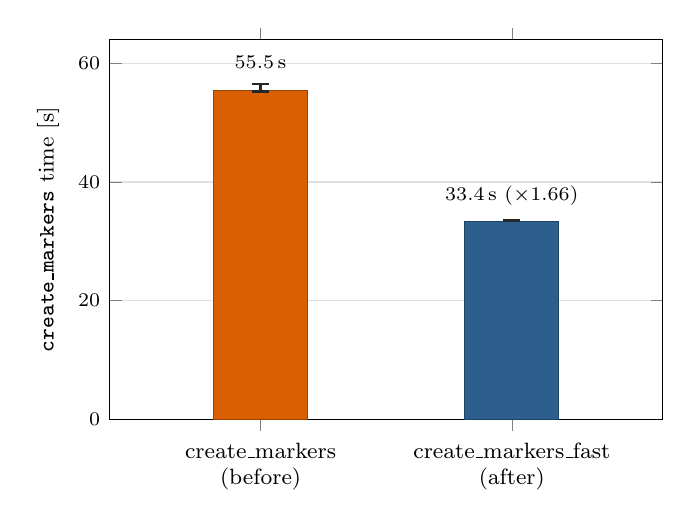
\begin{tikzpicture}
\begin{axis}[
    ybar,
    width=8.6cm, height=6.4cm,
    bar width=34pt,
    xmin=-0.6, xmax=1.6,
    xtick={0,1},
    xticklabels={\snakecase{create\_markers}\\(before),\snakecase{create\_markers\_fast}\\(after)},
    xticklabel style={font=\footnotesize, align=center, yshift=-0.2ex},
    ymin=0, ymax=64,
    ylabel={\texttt{create\_markers} time [s]},
    ylabel style={font=\footnotesize},
    tick label style={font=\scriptsize},
    ymajorgrids=true,
    major grid style={black!12},
    error bars/error bar style={black!85, line width=0.8pt},
    error bars/error mark options={
      mark size=3pt, rotate=90, line width=0.8pt, black!85,
    },
]
  \addplot+[
    ybar, bar shift=0pt, fill=cmbefore, draw=cmbefore!70!black, line width=0.4pt,
    error bars/.cd, y dir=both, y explicit,
  ] table[row sep=\\, x=x, y=y, y error plus=ep, y error minus=em] {
    x y ep em \\
    0 55.4791 1.1148 0.1899 \\
  };
  \addplot+[
    ybar, bar shift=0pt, fill=cmafter, draw=cmafter!70!black, line width=0.4pt,
    error bars/.cd, y dir=both, y explicit,
  ] table[row sep=\\, x=x, y=y, y error plus=ep, y error minus=em] {
    x y ep em \\
    1 33.3722 0.1328 0.0000 \\
  };

  % One label per bar, above the whisker cap: median value, and (for "after")
  % the speedup relative to "before" -- kept as a single node per bar rather
  % than two stacked ones, since the whisker span is only ~1s/~0.1s against a
  % 0-64s axis and two separately-anchored nodes there collide.
  \node[font=\scriptsize, anchor=south, yshift=2pt]
    at (axis cs:0,56.5939) {55.5\,s};
  \node[font=\scriptsize, anchor=south, yshift=2pt]
    at (axis cs:1,33.5050) {33.4\,s ($\times$1.66)};
\end{axis}
\end{tikzpicture}

\caption[\texttt{create\_markers} speedup from bulk ray collection]{\textbf{\snakecase{create\_markers} vs.\ \snakecase{create\_markers\_fast} wall time, 6VYB (test1).} Median over 3 runs, whiskers spanning fastest to slowest; the label above each bar is that median in seconds, with the speedup relative to \snakecase{create\_markers} in parentheses. \snakecase{create\_markers\_fast} collects all needed rays first with \snakecase{ensure\_ray}, then casts and distributes them in one bulk pass before classification (Section~\ref{sec:implementation-host-side-create-markers}). Measured on the local system (Table~\ref{tab:test-systems}).}
\label{fig:create-markers-speedup}
\end{figure}

%  Needs \usepackage{pgfplots} in the preamble.
% ------------------------------------------------------------------------
\pgfplotsset{compat=1.16}

\definecolor{cmbefore}{HTML}{D95F02}
\definecolor{cmafter}{HTML}{2C5F8D}

\begin{figure}[!htb]
\centering
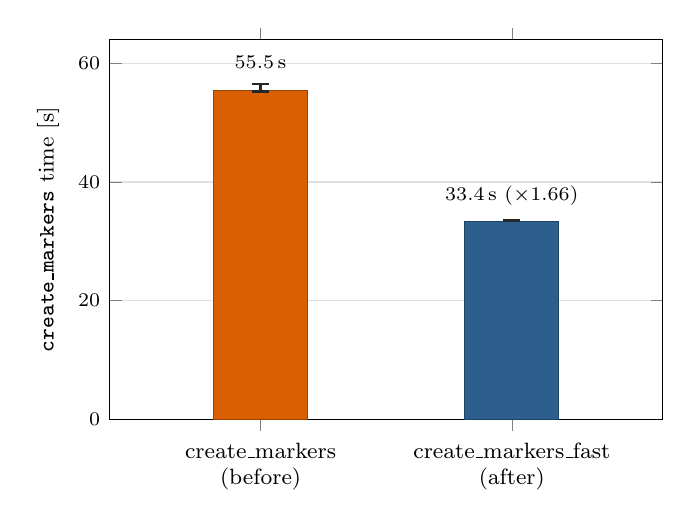
\begin{tikzpicture}
\begin{axis}[
    ybar,
    width=8.6cm, height=6.4cm,
    bar width=34pt,
    xmin=-0.6, xmax=1.6,
    xtick={0,1},
    xticklabels={\snakecase{create\_markers}\\(before),\snakecase{create\_markers\_fast}\\(after)},
    xticklabel style={font=\footnotesize, align=center, yshift=-0.2ex},
    ymin=0, ymax=64,
    ylabel={\texttt{create\_markers} time [s]},
    ylabel style={font=\footnotesize},
    tick label style={font=\scriptsize},
    ymajorgrids=true,
    major grid style={black!12},
    error bars/error bar style={black!85, line width=0.8pt},
    error bars/error mark options={
      mark size=3pt, rotate=90, line width=0.8pt, black!85,
    },
]
  \addplot+[
    ybar, bar shift=0pt, fill=cmbefore, draw=cmbefore!70!black, line width=0.4pt,
    error bars/.cd, y dir=both, y explicit,
  ] table[row sep=\\, x=x, y=y, y error plus=ep, y error minus=em] {
    x y ep em \\
    0 55.4791 1.1148 0.1899 \\
  };
  \addplot+[
    ybar, bar shift=0pt, fill=cmafter, draw=cmafter!70!black, line width=0.4pt,
    error bars/.cd, y dir=both, y explicit,
  ] table[row sep=\\, x=x, y=y, y error plus=ep, y error minus=em] {
    x y ep em \\
    1 33.3722 0.1328 0.0000 \\
  };

  % One label per bar, above the whisker cap: median value, and (for "after")
  % the speedup relative to "before" -- kept as a single node per bar rather
  % than two stacked ones, since the whisker span is only ~1s/~0.1s against a
  % 0-64s axis and two separately-anchored nodes there collide.
  \node[font=\scriptsize, anchor=south, yshift=2pt]
    at (axis cs:0,56.5939) {55.5\,s};
  \node[font=\scriptsize, anchor=south, yshift=2pt]
    at (axis cs:1,33.5050) {33.4\,s ($\times$1.66)};
\end{axis}
\end{tikzpicture}

\caption[\texttt{create\_markers} speedup from bulk ray collection]{\textbf{\snakecase{create\_markers} vs.\ \snakecase{create\_markers\_fast} wall time, 6VYB (test1).} Median over 3 runs, whiskers spanning fastest to slowest; the label above each bar is that median in seconds, with the speedup relative to \snakecase{create\_markers} in parentheses. \snakecase{create\_markers\_fast} collects all needed rays first with \snakecase{ensure\_ray}, then casts and distributes them in one bulk pass before classification (Section~\ref{sec:implementation-host-side-create-markers}). Measured on the local system (Table~\ref{tab:test-systems}).}
\label{fig:create-markers-speedup}
\end{figure}

%  Needs \usepackage{pgfplots} in the preamble.
% ------------------------------------------------------------------------
\pgfplotsset{compat=1.16}

\definecolor{cmbefore}{HTML}{D95F02}
\definecolor{cmafter}{HTML}{2C5F8D}

\begin{figure}[!htb]
\centering
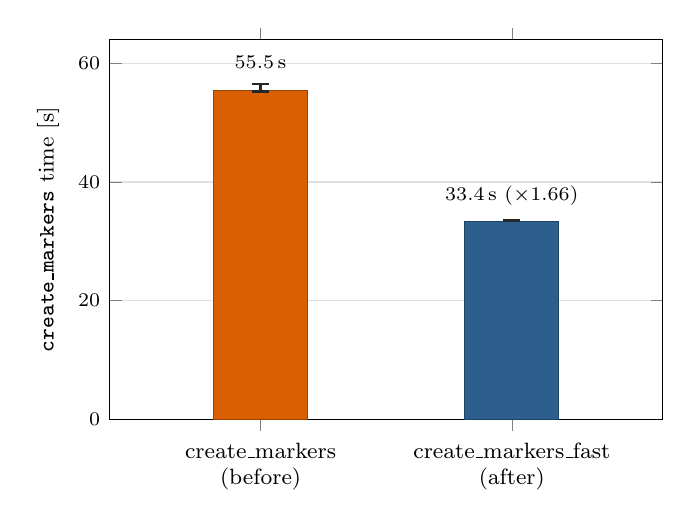
\begin{tikzpicture}
\begin{axis}[
    ybar,
    width=8.6cm, height=6.4cm,
    bar width=34pt,
    xmin=-0.6, xmax=1.6,
    xtick={0,1},
    xticklabels={\snakecase{create\_markers}\\(before),\snakecase{create\_markers\_fast}\\(after)},
    xticklabel style={font=\footnotesize, align=center, yshift=-0.2ex},
    ymin=0, ymax=64,
    ylabel={\texttt{create\_markers} time [s]},
    ylabel style={font=\footnotesize},
    tick label style={font=\scriptsize},
    ymajorgrids=true,
    major grid style={black!12},
    error bars/error bar style={black!85, line width=0.8pt},
    error bars/error mark options={
      mark size=3pt, rotate=90, line width=0.8pt, black!85,
    },
]
  \addplot+[
    ybar, bar shift=0pt, fill=cmbefore, draw=cmbefore!70!black, line width=0.4pt,
    error bars/.cd, y dir=both, y explicit,
  ] table[row sep=\\, x=x, y=y, y error plus=ep, y error minus=em] {
    x y ep em \\
    0 55.4791 1.1148 0.1899 \\
  };
  \addplot+[
    ybar, bar shift=0pt, fill=cmafter, draw=cmafter!70!black, line width=0.4pt,
    error bars/.cd, y dir=both, y explicit,
  ] table[row sep=\\, x=x, y=y, y error plus=ep, y error minus=em] {
    x y ep em \\
    1 33.3722 0.1328 0.0000 \\
  };

  % One label per bar, above the whisker cap: median value, and (for "after")
  % the speedup relative to "before" -- kept as a single node per bar rather
  % than two stacked ones, since the whisker span is only ~1s/~0.1s against a
  % 0-64s axis and two separately-anchored nodes there collide.
  \node[font=\scriptsize, anchor=south, yshift=2pt]
    at (axis cs:0,56.5939) {55.5\,s};
  \node[font=\scriptsize, anchor=south, yshift=2pt]
    at (axis cs:1,33.5050) {33.4\,s ($\times$1.66)};
\end{axis}
\end{tikzpicture}

\caption[\texttt{create\_markers} speedup from bulk ray collection]{\textbf{\snakecase{create\_markers} vs.\ \snakecase{create\_markers\_fast} wall time, 6VYB (test1).} Median over 3 runs, whiskers spanning fastest to slowest; the label above each bar is that median in seconds, with the speedup relative to \snakecase{create\_markers} in parentheses. \snakecase{create\_markers\_fast} collects all needed rays first with \snakecase{ensure\_ray}, then casts and distributes them in one bulk pass before classification (Section~\ref{sec:implementation-host-side-create-markers}). Measured on the local system (Table~\ref{tab:test-systems}).}
\label{fig:create-markers-speedup}
\end{figure}

\FloatBarrier

\subsection{BIMPP}
\label{sec:evaluation-results-bimpp}

I forked the official BIMPP repository to do my implementations, and built and installed on my local system.
I also shipped my local build with the Singularity container instead of the official one.
Using git I could quickly switch between the official version and my own if needed.

\subsubsection{sparse\_matrix\_template}

Figure~\ref{fig:bimpp-memory-fix} shows the reduction of the memory consumption on rank 1 for 6VYB (test1).
The move from \snakecase{std::map} to \snakecase{boost::container::flat\_map} lead to a 2.14x reduction of the host memory usage during \snakecase{assemble\_system\_matrix}, which was better than the predicted 2x reduction.
Upon closer inspection, the swap shrinks the per-entry storage \textit{and} the outer vector of row handles, independently.
Being the most memory intensive step in the entire NGPB pipeline, it had a great effect on the total memory consumption as well, reducing it by 1.5x.
The remaining memory utilization of around 2.02GB, coming mostly from the p8est mesh, is unchanged.
The totals are Heaptrack's peak heap memory consumption over the whole run, while the numbers for \snakecase{assemble\_system\_matrix} are the sum its allocations. 
This change had no impact on accuracy, however it has slightly positive impact on the stage time of \snakecase{assemble\_system\_matrix}, going from roughly 22 seconds to 20.

I have to clarify that this did not fix BIMPP's general issue of storing the entire global row of a distributed sparse matrix on every rank.
However, that would have required major architectural changes to BIMPP.
The swap was a non-intrusive band-aid-fix.

% ------------------------------------------------------------------------
%  sparse_matrix_template memory fix: std::map -> boost::container::flat_map.
%  Hand-authored from the 2026-09-01 matched pair (rank 1, 6VYB, 4 MPI ranks,
%  LIS -- verified in both captures, not taken from the filenames):
%  test1/profiles/ngpb.rank1.zst (std::map, captured 17:38 against a
%  reinstalled base bimpp) and the cook of the 13:43 capture (flat_map).
%  Same config, VERIFIED -- not assumed. The container-independent mesh proxies
%  are identical digit for digit across the pair:
%      num_local_nodes  813.29M over 726488 calls   (both)
%      create_density_map    84882360 calls         (both)
%  and the whole 7.69M difference in total allocation count is accounted for by
%  the 7.71M difference at the assembly container site, to within 20k of 599M.
%  The superseded pair (base.zst / opt.amgx.zst, Apr+May) was NOT same-config:
%  those proxies differed by 13.5%, which inflated the drop. Do not go back.
%
%  TOTALS are heaptrack_print / Summary "peak heap memory consumption", NOT the
%  Top-Down "main" row. Top-Down main is not the process peak -- the tree has
%  several roots (main, _start, __clone3) and merged-node peaks are documented
%  as "not correct"; captures can also unwind to different depths and root the
%  same allocation differently, which silently drops it from main's subtree.
%  ASSEMBLY bars sum the peak consumers heaptrack_print reports under
%  --filter-bt-function assemble_system_matrix. Two sites dominate:
%      entry storage      2.40G -> 1.02G   (RB-tree nodes -> flat vectors)
%      row-handle array   1.34G -> 672.21M (one alloc; 48B -> 24B per row)
%  everything else is under 60MB. This inherits the merged-peak caveat (maxima
%  at different instants), unlike the totals, which are exact.
%  See [[project_bimpp_memory]].
%  Include with % ------------------------------------------------------------------------
%  sparse_matrix_template memory fix: std::map -> boost::container::flat_map.
%  Hand-authored from the 2026-09-01 matched pair (rank 1, 6VYB, 4 MPI ranks,
%  LIS -- verified in both captures, not taken from the filenames):
%  test1/profiles/ngpb.rank1.zst (std::map, captured 17:38 against a
%  reinstalled base bimpp) and the cook of the 13:43 capture (flat_map).
%  Same config, VERIFIED -- not assumed. The container-independent mesh proxies
%  are identical digit for digit across the pair:
%      num_local_nodes  813.29M over 726488 calls   (both)
%      create_density_map    84882360 calls         (both)
%  and the whole 7.69M difference in total allocation count is accounted for by
%  the 7.71M difference at the assembly container site, to within 20k of 599M.
%  The superseded pair (base.zst / opt.amgx.zst, Apr+May) was NOT same-config:
%  those proxies differed by 13.5%, which inflated the drop. Do not go back.
%
%  TOTALS are heaptrack_print / Summary "peak heap memory consumption", NOT the
%  Top-Down "main" row. Top-Down main is not the process peak -- the tree has
%  several roots (main, _start, __clone3) and merged-node peaks are documented
%  as "not correct"; captures can also unwind to different depths and root the
%  same allocation differently, which silently drops it from main's subtree.
%  ASSEMBLY bars sum the peak consumers heaptrack_print reports under
%  --filter-bt-function assemble_system_matrix. Two sites dominate:
%      entry storage      2.40G -> 1.02G   (RB-tree nodes -> flat vectors)
%      row-handle array   1.34G -> 672.21M (one alloc; 48B -> 24B per row)
%  everything else is under 60MB. This inherits the merged-peak caveat (maxima
%  at different instants), unlike the totals, which are exact.
%  See [[project_bimpp_memory]].
%  Include with % ------------------------------------------------------------------------
%  sparse_matrix_template memory fix: std::map -> boost::container::flat_map.
%  Hand-authored from the 2026-09-01 matched pair (rank 1, 6VYB, 4 MPI ranks,
%  LIS -- verified in both captures, not taken from the filenames):
%  test1/profiles/ngpb.rank1.zst (std::map, captured 17:38 against a
%  reinstalled base bimpp) and the cook of the 13:43 capture (flat_map).
%  Same config, VERIFIED -- not assumed. The container-independent mesh proxies
%  are identical digit for digit across the pair:
%      num_local_nodes  813.29M over 726488 calls   (both)
%      create_density_map    84882360 calls         (both)
%  and the whole 7.69M difference in total allocation count is accounted for by
%  the 7.71M difference at the assembly container site, to within 20k of 599M.
%  The superseded pair (base.zst / opt.amgx.zst, Apr+May) was NOT same-config:
%  those proxies differed by 13.5%, which inflated the drop. Do not go back.
%
%  TOTALS are heaptrack_print / Summary "peak heap memory consumption", NOT the
%  Top-Down "main" row. Top-Down main is not the process peak -- the tree has
%  several roots (main, _start, __clone3) and merged-node peaks are documented
%  as "not correct"; captures can also unwind to different depths and root the
%  same allocation differently, which silently drops it from main's subtree.
%  ASSEMBLY bars sum the peak consumers heaptrack_print reports under
%  --filter-bt-function assemble_system_matrix. Two sites dominate:
%      entry storage      2.40G -> 1.02G   (RB-tree nodes -> flat vectors)
%      row-handle array   1.34G -> 672.21M (one alloc; 48B -> 24B per row)
%  everything else is under 60MB. This inherits the merged-peak caveat (maxima
%  at different instants), unlike the totals, which are exact.
%  See [[project_bimpp_memory]].
%  Include with \input{figures/bimpp_memory_fix}
%  Needs \usepackage{pgfplots} in the preamble.
% ------------------------------------------------------------------------
\pgfplotsset{compat=1.16}

\definecolor{memtotal}{HTML}{2C5F8D}
\definecolor{memassemble}{HTML}{9DC3E0}

\begin{figure}[!htb]
\centering
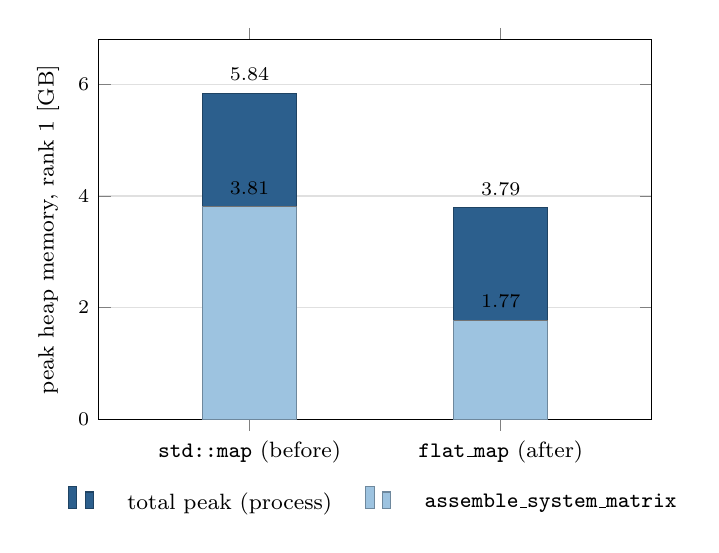
\begin{tikzpicture}
\begin{axis}[
    ybar,
    width=8.6cm, height=6.4cm,
    bar width=34pt,
    xmin=-0.6, xmax=1.6,
    xtick={0,1},
    xticklabels={\texttt{std::map} (before),\texttt{flat\_map} (after)},
    xticklabel style={font=\footnotesize, align=center},
    ymin=0, ymax=6.8,
    ylabel={peak heap memory, rank 1 [GB]},
    ylabel style={font=\footnotesize},
    tick label style={font=\scriptsize},
    ymajorgrids=true,
    major grid style={black!12},
    legend style={
      at={(0.5,-0.16)}, anchor=north, draw=none,
      legend columns=2, font=\footnotesize, column sep=1em,
    },
]
  % Overlay, not stack: assemble_system_matrix is a subset of the total, so the
  % second series is drawn at the same x position (bar shift=0pt) on top of the
  % first, covering its lower portion. The remaining visible strip of memtotal
  % above the seam is "everything in main's peak that is not assembly".
  \addplot+[
    ybar, bar shift=0pt, fill=memtotal, draw=memtotal!70!black, line width=0.4pt,
  ] coordinates {(0,5.84) (1,3.79)};
  \addlegendentry{total peak (process)}
  \addplot+[
    ybar, bar shift=0pt, fill=memassemble, draw=memassemble!70!black, line width=0.4pt,
  ] coordinates {(0,3.81) (1,1.77)};
  \addlegendentry{\texttt{assemble\_system\_matrix}}

  % Value labels: total at the bar top, assemble at the seam between the two
  % colors, with a short cap line marking the seam itself.
  \node[font=\scriptsize, anchor=south, yshift=1pt] at (axis cs:0,5.84) {5.84};
  \node[font=\scriptsize, anchor=south, yshift=1pt] at (axis cs:1,3.79) {3.79};
  \draw[black!55, line width=0.6pt] ([xshift=-17pt]axis cs:0,3.81) -- ([xshift=17pt]axis cs:0,3.81);
  \draw[black!55, line width=0.6pt] ([xshift=-17pt]axis cs:1,1.77) -- ([xshift=17pt]axis cs:1,1.77);
  \node[font=\scriptsize, anchor=south, yshift=1pt] at (axis cs:0,3.81) {3.81};
  \node[font=\scriptsize, anchor=south, yshift=1pt] at (axis cs:1,1.77) {1.77};
\end{axis}
\end{tikzpicture}

\caption[Sparse matrix memory fix]{\textbf{Effect of the \texttt{sparse\_matrix\_template} fix on peak host memory, 6VYB, rank 1.} The process-wide peak heap consumption against the peak attributable to \snakecase{assemble\_system\_matrix} (Section~\ref{sec:evaluation-experimental-setup-comparing-memory-utilization}). Both captures use the LIS solver, measured on the local system (Table~\ref{tab:test-systems}).}
\label{fig:bimpp-memory-fix}
\end{figure}

%  Needs \usepackage{pgfplots} in the preamble.
% ------------------------------------------------------------------------
\pgfplotsset{compat=1.16}

\definecolor{memtotal}{HTML}{2C5F8D}
\definecolor{memassemble}{HTML}{9DC3E0}

\begin{figure}[!htb]
\centering
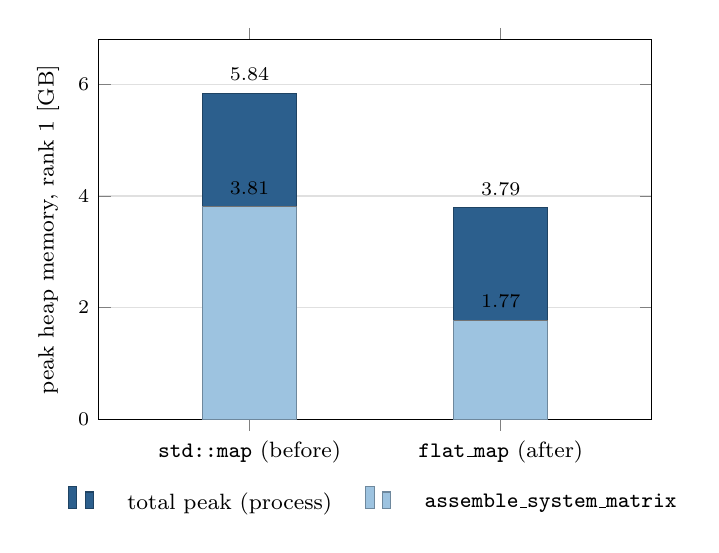
\begin{tikzpicture}
\begin{axis}[
    ybar,
    width=8.6cm, height=6.4cm,
    bar width=34pt,
    xmin=-0.6, xmax=1.6,
    xtick={0,1},
    xticklabels={\texttt{std::map} (before),\texttt{flat\_map} (after)},
    xticklabel style={font=\footnotesize, align=center},
    ymin=0, ymax=6.8,
    ylabel={peak heap memory, rank 1 [GB]},
    ylabel style={font=\footnotesize},
    tick label style={font=\scriptsize},
    ymajorgrids=true,
    major grid style={black!12},
    legend style={
      at={(0.5,-0.16)}, anchor=north, draw=none,
      legend columns=2, font=\footnotesize, column sep=1em,
    },
]
  % Overlay, not stack: assemble_system_matrix is a subset of the total, so the
  % second series is drawn at the same x position (bar shift=0pt) on top of the
  % first, covering its lower portion. The remaining visible strip of memtotal
  % above the seam is "everything in main's peak that is not assembly".
  \addplot+[
    ybar, bar shift=0pt, fill=memtotal, draw=memtotal!70!black, line width=0.4pt,
  ] coordinates {(0,5.84) (1,3.79)};
  \addlegendentry{total peak (process)}
  \addplot+[
    ybar, bar shift=0pt, fill=memassemble, draw=memassemble!70!black, line width=0.4pt,
  ] coordinates {(0,3.81) (1,1.77)};
  \addlegendentry{\texttt{assemble\_system\_matrix}}

  % Value labels: total at the bar top, assemble at the seam between the two
  % colors, with a short cap line marking the seam itself.
  \node[font=\scriptsize, anchor=south, yshift=1pt] at (axis cs:0,5.84) {5.84};
  \node[font=\scriptsize, anchor=south, yshift=1pt] at (axis cs:1,3.79) {3.79};
  \draw[black!55, line width=0.6pt] ([xshift=-17pt]axis cs:0,3.81) -- ([xshift=17pt]axis cs:0,3.81);
  \draw[black!55, line width=0.6pt] ([xshift=-17pt]axis cs:1,1.77) -- ([xshift=17pt]axis cs:1,1.77);
  \node[font=\scriptsize, anchor=south, yshift=1pt] at (axis cs:0,3.81) {3.81};
  \node[font=\scriptsize, anchor=south, yshift=1pt] at (axis cs:1,1.77) {1.77};
\end{axis}
\end{tikzpicture}

\caption[Sparse matrix memory fix]{\textbf{Effect of the \texttt{sparse\_matrix\_template} fix on peak host memory, 6VYB, rank 1.} The process-wide peak heap consumption against the peak attributable to \snakecase{assemble\_system\_matrix} (Section~\ref{sec:evaluation-experimental-setup-comparing-memory-utilization}). Both captures use the LIS solver, measured on the local system (Table~\ref{tab:test-systems}).}
\label{fig:bimpp-memory-fix}
\end{figure}

%  Needs \usepackage{pgfplots} in the preamble.
% ------------------------------------------------------------------------
\pgfplotsset{compat=1.16}

\definecolor{memtotal}{HTML}{2C5F8D}
\definecolor{memassemble}{HTML}{9DC3E0}

\begin{figure}[!htb]
\centering
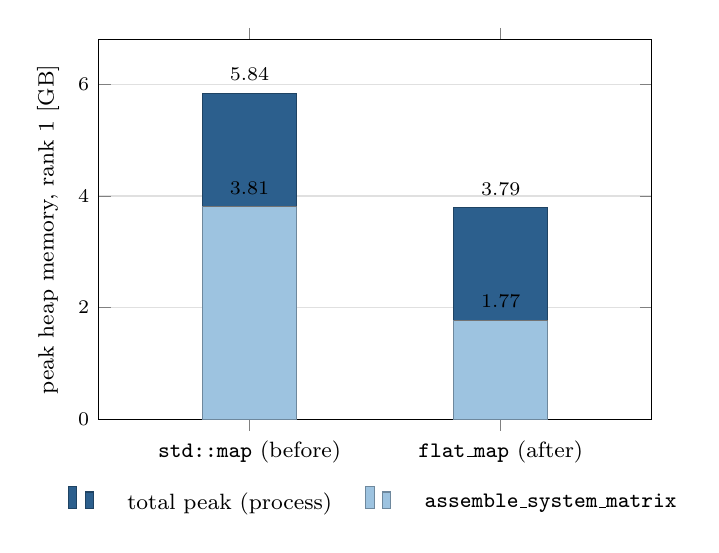
\begin{tikzpicture}
\begin{axis}[
    ybar,
    width=8.6cm, height=6.4cm,
    bar width=34pt,
    xmin=-0.6, xmax=1.6,
    xtick={0,1},
    xticklabels={\texttt{std::map} (before),\texttt{flat\_map} (after)},
    xticklabel style={font=\footnotesize, align=center},
    ymin=0, ymax=6.8,
    ylabel={peak heap memory, rank 1 [GB]},
    ylabel style={font=\footnotesize},
    tick label style={font=\scriptsize},
    ymajorgrids=true,
    major grid style={black!12},
    legend style={
      at={(0.5,-0.16)}, anchor=north, draw=none,
      legend columns=2, font=\footnotesize, column sep=1em,
    },
]
  % Overlay, not stack: assemble_system_matrix is a subset of the total, so the
  % second series is drawn at the same x position (bar shift=0pt) on top of the
  % first, covering its lower portion. The remaining visible strip of memtotal
  % above the seam is "everything in main's peak that is not assembly".
  \addplot+[
    ybar, bar shift=0pt, fill=memtotal, draw=memtotal!70!black, line width=0.4pt,
  ] coordinates {(0,5.84) (1,3.79)};
  \addlegendentry{total peak (process)}
  \addplot+[
    ybar, bar shift=0pt, fill=memassemble, draw=memassemble!70!black, line width=0.4pt,
  ] coordinates {(0,3.81) (1,1.77)};
  \addlegendentry{\texttt{assemble\_system\_matrix}}

  % Value labels: total at the bar top, assemble at the seam between the two
  % colors, with a short cap line marking the seam itself.
  \node[font=\scriptsize, anchor=south, yshift=1pt] at (axis cs:0,5.84) {5.84};
  \node[font=\scriptsize, anchor=south, yshift=1pt] at (axis cs:1,3.79) {3.79};
  \draw[black!55, line width=0.6pt] ([xshift=-17pt]axis cs:0,3.81) -- ([xshift=17pt]axis cs:0,3.81);
  \draw[black!55, line width=0.6pt] ([xshift=-17pt]axis cs:1,1.77) -- ([xshift=17pt]axis cs:1,1.77);
  \node[font=\scriptsize, anchor=south, yshift=1pt] at (axis cs:0,3.81) {3.81};
  \node[font=\scriptsize, anchor=south, yshift=1pt] at (axis cs:1,1.77) {1.77};
\end{axis}
\end{tikzpicture}

\caption[Sparse matrix memory fix]{\textbf{Effect of the \texttt{sparse\_matrix\_template} fix on peak host memory, 6VYB, rank 1.} The process-wide peak heap consumption against the peak attributable to \snakecase{assemble\_system\_matrix} (Section~\ref{sec:evaluation-experimental-setup-comparing-memory-utilization}). Both captures use the LIS solver, measured on the local system (Table~\ref{tab:test-systems}).}
\label{fig:bimpp-memory-fix}
\end{figure}


\subsubsection{bim3a\_solution\_with\_ghosts}

My optimized \snakecase{bim3a_solution_with_ghosts} reduced the time taken for 6YVB from 10 seconds to just 60 milliseconds, which is an extreme speedup of almost 170x.
This moves it from being a significant contributor of the overall time to basically negligible.
Being used at the end of every solver, and twice inside \snakecase{create_density_map}, this removed roughly 30 from the overall total time for the full NGPB pipeline, \snakecase{create_density_map} alone shortening from 24 seconds to just 2.5 seconds.
This change also had no impact on accuracy.
The only thing this costs is that the function is less agnostic to p4est, which means nothing in a library that otherwise solely relies on it.

\FloatBarrier

\subsection{Baseline}
\label{evaluation-results-baseline}

I got slightly different results for the two analytical tests than the NGPB paper \cite{diflorio2025nextgenpb}.
Some relative errors slightly are lower for me, while others slightly higher.
The order or magnitude stayed the same across the board.
The differences are shown in Table~\ref{tab:baseline-accuracy}.
Interestingly, the triangulation-fix had no impact on these test.
The relative errors were exactly identical.

Although AMGX was set to a lower residual, it did not increase accuracy.
In fact is worsened the polarization error for the Kirkwood sphere test slightly when compared to the LIS result, which is still way better than the result from the paper.
AMGX did genuinely reach a lower residual (1.195268e-09) than LIS (5.921088e-07), suggesting this is not a limitation of the software, but rather limitation of the mathematical method.
It also might explain why the authors of NGPB had LIS set to a residual of 1e-6: at this value the accuracy already bottoms out.
I set my personal result with LIS as the accuracy requirement for FMM.
For AMGX I accepted the slight loss, as it is clearly very small.

% ------------------------------------------------------------------------
%  Baseline (host, triangulation-fix) accuracy on the two analytical test
%  systems, next to the values printed in the NGPB paper.
%  "NGPB paper" rows are Table~\ref{tab:ngpb-error-magnitudes} (relative error
%  magnitudes only, no sign given). "baseline (LIS/AMGX)" rows are relative
%  error against the exact analytical reference
%  (Table~\ref{tab:ngpb-analytical-values}), from the user's own test3/test4
%  runs (config: Table~\ref{tab:test-cases}) with linear_solver set to lis and
%  amgx respectively, signed as reported -- the 30-sphere polarization runs
%  came back negative.
%  Hand-authored, no backing log file (console output, not captured to disk).
%  Include with % ------------------------------------------------------------------------
%  Baseline (host, triangulation-fix) accuracy on the two analytical test
%  systems, next to the values printed in the NGPB paper.
%  "NGPB paper" rows are Table~\ref{tab:ngpb-error-magnitudes} (relative error
%  magnitudes only, no sign given). "baseline (LIS/AMGX)" rows are relative
%  error against the exact analytical reference
%  (Table~\ref{tab:ngpb-analytical-values}), from the user's own test3/test4
%  runs (config: Table~\ref{tab:test-cases}) with linear_solver set to lis and
%  amgx respectively, signed as reported -- the 30-sphere polarization runs
%  came back negative.
%  Hand-authored, no backing log file (console output, not captured to disk).
%  Include with % ------------------------------------------------------------------------
%  Baseline (host, triangulation-fix) accuracy on the two analytical test
%  systems, next to the values printed in the NGPB paper.
%  "NGPB paper" rows are Table~\ref{tab:ngpb-error-magnitudes} (relative error
%  magnitudes only, no sign given). "baseline (LIS/AMGX)" rows are relative
%  error against the exact analytical reference
%  (Table~\ref{tab:ngpb-analytical-values}), from the user's own test3/test4
%  runs (config: Table~\ref{tab:test-cases}) with linear_solver set to lis and
%  amgx respectively, signed as reported -- the 30-sphere polarization runs
%  came back negative.
%  Hand-authored, no backing log file (console output, not captured to disk).
%  Include with \input{figures/baseline_accuracy_table}
%  Needs \usepackage{booktabs}.
% ------------------------------------------------------------------------
\begin{table}[!htb]
\centering
\footnotesize
\caption[Baseline vs.\ NGPB analytical accuracy]{\textbf{Relative error against the exact analytical reference (Table~\ref{tab:ngpb-analytical-values}), baseline vs.\ NGPB paper.} \emph{NGPB paper} reproduces Table~\ref{tab:ngpb-error-magnitudes}; \emph{baseline (LIS/AMGX)} is my own run of the same test system (Table~\ref{tab:test-cases}) with each linear solver.}
\label{tab:baseline-accuracy}
\begin{tabular}{llrrr}
\toprule
system & source & polarization & ionic & total \\
\midrule
Kirkwood sphere & NGPB paper & $7.38\times10^{-10}$ & $3.39\times10^{-2}$ & $1.72\times10^{-4}$ \\
 & baseline (LIS) & $1.246641\times10^{-10}$ & $3.358548\times10^{-2}$ & $1.702569\times10^{-4}$ \\
 & baseline (AMGX) & $1.456175\times10^{-10}$ & $3.358548\times10^{-2}$ & $1.702569\times10^{-4}$ \\
\midrule
30-sphere & NGPB paper & $4.16\times10^{-5}$ & $1.39\times10^{-2}$ & $7.46\times10^{-4}$ \\
 & baseline (LIS) & $-7.037554\times10^{-5}$ & $1.355291\times10^{-2}$ & $5.866853\times10^{-4}$ \\
 & baseline (AMGX) & $-7.037566\times10^{-5}$ & $1.355334\times10^{-2}$ & $5.867130\times10^{-4}$ \\
\bottomrule
\end{tabular}
\end{table}

%  Needs \usepackage{booktabs}.
% ------------------------------------------------------------------------
\begin{table}[!htb]
\centering
\footnotesize
\caption[Baseline vs.\ NGPB analytical accuracy]{\textbf{Relative error against the exact analytical reference (Table~\ref{tab:ngpb-analytical-values}), baseline vs.\ NGPB paper.} \emph{NGPB paper} reproduces Table~\ref{tab:ngpb-error-magnitudes}; \emph{baseline (LIS/AMGX)} is my own run of the same test system (Table~\ref{tab:test-cases}) with each linear solver.}
\label{tab:baseline-accuracy}
\begin{tabular}{llrrr}
\toprule
system & source & polarization & ionic & total \\
\midrule
Kirkwood sphere & NGPB paper & $7.38\times10^{-10}$ & $3.39\times10^{-2}$ & $1.72\times10^{-4}$ \\
 & baseline (LIS) & $1.246641\times10^{-10}$ & $3.358548\times10^{-2}$ & $1.702569\times10^{-4}$ \\
 & baseline (AMGX) & $1.456175\times10^{-10}$ & $3.358548\times10^{-2}$ & $1.702569\times10^{-4}$ \\
\midrule
30-sphere & NGPB paper & $4.16\times10^{-5}$ & $1.39\times10^{-2}$ & $7.46\times10^{-4}$ \\
 & baseline (LIS) & $-7.037554\times10^{-5}$ & $1.355291\times10^{-2}$ & $5.866853\times10^{-4}$ \\
 & baseline (AMGX) & $-7.037566\times10^{-5}$ & $1.355334\times10^{-2}$ & $5.867130\times10^{-4}$ \\
\bottomrule
\end{tabular}
\end{table}

%  Needs \usepackage{booktabs}.
% ------------------------------------------------------------------------
\begin{table}[!htb]
\centering
\footnotesize
\caption[Baseline vs.\ NGPB analytical accuracy]{\textbf{Relative error against the exact analytical reference (Table~\ref{tab:ngpb-analytical-values}), baseline vs.\ NGPB paper.} \emph{NGPB paper} reproduces Table~\ref{tab:ngpb-error-magnitudes}; \emph{baseline (LIS/AMGX)} is my own run of the same test system (Table~\ref{tab:test-cases}) with each linear solver.}
\label{tab:baseline-accuracy}
\begin{tabular}{llrrr}
\toprule
system & source & polarization & ionic & total \\
\midrule
Kirkwood sphere & NGPB paper & $7.38\times10^{-10}$ & $3.39\times10^{-2}$ & $1.72\times10^{-4}$ \\
 & baseline (LIS) & $1.246641\times10^{-10}$ & $3.358548\times10^{-2}$ & $1.702569\times10^{-4}$ \\
 & baseline (AMGX) & $1.456175\times10^{-10}$ & $3.358548\times10^{-2}$ & $1.702569\times10^{-4}$ \\
\midrule
30-sphere & NGPB paper & $4.16\times10^{-5}$ & $1.39\times10^{-2}$ & $7.46\times10^{-4}$ \\
 & baseline (LIS) & $-7.037554\times10^{-5}$ & $1.355291\times10^{-2}$ & $5.866853\times10^{-4}$ \\
 & baseline (AMGX) & $-7.037566\times10^{-5}$ & $1.355334\times10^{-2}$ & $5.867130\times10^{-4}$ \\
\bottomrule
\end{tabular}
\end{table}

\FloatBarrier

\subsection{Linear Equation Solver}
\label{sec:evaluation-results-lin-eq-solver}

\subsubsection{Local System}

Figure~\ref{fig:solver-bench} compares the total stage time of the LIS and AMGX path for 1CCM, 6VYB and 1VSZ running on the local system.
Despite being set to a much smaller residual, the default configuration for AMGX manages to beat LIS at every sample size on the local system.
For 1VSZ and 6VYB, the speedup was 10x, while for 1CCM it was much smaller.
The tuned AMGX configuration runs faster than the default one, also at every sample size.
This only tells half of the story: Table~\ref{tab:solver-bench} breaks the stage time down into the host time and AMGX's actual solve time.
As LIS runs entirely on the CPU, its entire time attributed to the host.
This shows that the CPU time for AMGX path, made up of the data gathering and transfer, is significant.

% ------------------------------------------------------------------------
%  Linear solver comparison (bench_sweep.py sweep A).
%  Generated by scripts/plot_solver_bench.py -- regenerate rather than edit.
%  Include with % ------------------------------------------------------------------------
%  Linear solver comparison (bench_sweep.py sweep A).
%  Generated by scripts/plot_solver_bench.py -- regenerate rather than edit.
%  Include with % ------------------------------------------------------------------------
%  Linear solver comparison (bench_sweep.py sweep A).
%  Generated by scripts/plot_solver_bench.py -- regenerate rather than edit.
%  Include with \input{figures/solver_bench}
%  Needs \usepackage{pgfplots} in the preamble.
% ------------------------------------------------------------------------
\input{figures/data/solver_bench_ref}

\pgfplotsset{compat=1.16}

% Keep only the rows whose column #1 equals #2.
\pgfplotsset{
  discard if not/.style 2 args={
    x filter/.code={%
      \edef\tempa{\thisrow{#1}}\edef\tempb{#2}%
      \ifx\tempa\tempb\else\def\pgfmathresult{inf}\fi
    }
  }
}

\definecolor{solverlis}{HTML}{D95F02}
\definecolor{solveramgx}{HTML}{9DC3E0}
\definecolor{solvercfg}{HTML}{2C5F8D}

\begin{figure}[!htb]
\centering
\begin{tikzpicture}
\begin{axis}[
    ybar,
    width=9.6cm, height=6.4cm,
    bar width=26pt,
    enlarge x limits=0.18,
    ymin=0, ymax=0.383123,
    ylabel={\solverMetric{} time [s]},
    ylabel style={font=\footnotesize},
    xtick={0,1,2},
    xticklabels={{LIS},{AMGX\\(default)},{AMGX\\(tuned)}},
    xmin=-0.7, xmax=2.7,
    xticklabel style={font=\footnotesize, align=center},
    tick label style={font=\scriptsize},
    ymajorgrids=true,
    major grid style={black!12},
    % Run-to-run spread is only a few percent, so the upper whisker is 1-2 mm and
    % the lower half is buried in the bar fill. Caps nearly as wide as the bar
    % are what make it read as an error bar rather than a stray tick.
    % T-caps. rotate=90 is required: pgfplots draws the cap perpendicular to the
    % error direction by itself, but any mark size given here clobbers that, and
    % the cap then renders vertically -- which reads as a longer whisker rather
    % than a wider cap. Setting error mark explicitly does not help; the rotation
    % is what matters.
    error bars/error bar style={black!85, line width=0.8pt},
    error bars/error mark options={
      mark size=6pt, rotate=90, line width=0.8pt, black!85,
    },
    every node near coord/.append style={
      font=\tiny, color=black!60, anchor=south, yshift=5pt,
    },
]
  \addplot+[
    ybar, bar shift=0pt, fill=solverlis, draw=solverlis!70!black, line width=0.4pt,
    nodes near coords, point meta=explicit symbolic,
    error bars/.cd, y dir=both, y explicit,
  ] table[x=idx, y=value, y error minus=em, y error plus=ep, meta=iters,
          discard if not={config}{lis}] {figures/data/solver_bench.dat};
  \addplot+[
    ybar, bar shift=0pt, fill=solveramgx, draw=solveramgx!70!black, line width=0.4pt,
    nodes near coords, point meta=explicit symbolic,
    error bars/.cd, y dir=both, y explicit,
  ] table[x=idx, y=value, y error minus=em, y error plus=ep, meta=iters,
          discard if not={config}{amgx}] {figures/data/solver_bench.dat};
  \addplot+[
    ybar, bar shift=0pt, fill=solvercfg, draw=solvercfg!70!black, line width=0.4pt,
    nodes near coords, point meta=explicit symbolic,
    error bars/.cd, y dir=both, y explicit,
  ] table[x=idx, y=value, y error minus=em, y error plus=ep, meta=iters,
          discard if not={config}{amgxcfg}] {figures/data/solver_bench.dat};

\end{axis}
\end{tikzpicture}

\caption[Linear solver comparison]{\textbf{Linear solver comparison on
    \solverMolecules{}.} Median \solverMetric{} time over \solverRepeats{} runs
    per configuration, with whiskers spanning the fastest and slowest of those
    runs; the small figure above each column is the iteration count. All three
    configurations use the same discretisation and the same energy path
    (\texttt{energy\_method\,=\,1}), so the bars differ only in the linear
    solver. Note that they do not all converge to the same residual --
    table~\ref{tab:solver-bench} gives the residual each one actually reached,
    without which the times are not comparable.}
\label{fig:solver-bench}
\end{figure}

%  Needs \usepackage{pgfplots} in the preamble.
% ------------------------------------------------------------------------
% generated by scripts/plot_solver_bench.py -- do not edit
\def\solverMetric{solve stage}
\def\solverRepeats{3}
\def\solverUnit{seconds}
\def\solverMolecules{1CCM, 6VYB, 1vsz}


\pgfplotsset{compat=1.16}

% Keep only the rows whose column #1 equals #2.
\pgfplotsset{
  discard if not/.style 2 args={
    x filter/.code={%
      \edef\tempa{\thisrow{#1}}\edef\tempb{#2}%
      \ifx\tempa\tempb\else\def\pgfmathresult{inf}\fi
    }
  }
}

\definecolor{solverlis}{HTML}{D95F02}
\definecolor{solveramgx}{HTML}{9DC3E0}
\definecolor{solvercfg}{HTML}{2C5F8D}

\begin{figure}[!htb]
\centering
\begin{tikzpicture}
\begin{axis}[
    ybar,
    width=9.6cm, height=6.4cm,
    bar width=26pt,
    enlarge x limits=0.18,
    ymin=0, ymax=0.383123,
    ylabel={\solverMetric{} time [s]},
    ylabel style={font=\footnotesize},
    xtick={0,1,2},
    xticklabels={{LIS},{AMGX\\(default)},{AMGX\\(tuned)}},
    xmin=-0.7, xmax=2.7,
    xticklabel style={font=\footnotesize, align=center},
    tick label style={font=\scriptsize},
    ymajorgrids=true,
    major grid style={black!12},
    % Run-to-run spread is only a few percent, so the upper whisker is 1-2 mm and
    % the lower half is buried in the bar fill. Caps nearly as wide as the bar
    % are what make it read as an error bar rather than a stray tick.
    % T-caps. rotate=90 is required: pgfplots draws the cap perpendicular to the
    % error direction by itself, but any mark size given here clobbers that, and
    % the cap then renders vertically -- which reads as a longer whisker rather
    % than a wider cap. Setting error mark explicitly does not help; the rotation
    % is what matters.
    error bars/error bar style={black!85, line width=0.8pt},
    error bars/error mark options={
      mark size=6pt, rotate=90, line width=0.8pt, black!85,
    },
    every node near coord/.append style={
      font=\tiny, color=black!60, anchor=south, yshift=5pt,
    },
]
  \addplot+[
    ybar, bar shift=0pt, fill=solverlis, draw=solverlis!70!black, line width=0.4pt,
    nodes near coords, point meta=explicit symbolic,
    error bars/.cd, y dir=both, y explicit,
  ] table[x=idx, y=value, y error minus=em, y error plus=ep, meta=iters,
          discard if not={config}{lis}] {figures/data/solver_bench.dat};
  \addplot+[
    ybar, bar shift=0pt, fill=solveramgx, draw=solveramgx!70!black, line width=0.4pt,
    nodes near coords, point meta=explicit symbolic,
    error bars/.cd, y dir=both, y explicit,
  ] table[x=idx, y=value, y error minus=em, y error plus=ep, meta=iters,
          discard if not={config}{amgx}] {figures/data/solver_bench.dat};
  \addplot+[
    ybar, bar shift=0pt, fill=solvercfg, draw=solvercfg!70!black, line width=0.4pt,
    nodes near coords, point meta=explicit symbolic,
    error bars/.cd, y dir=both, y explicit,
  ] table[x=idx, y=value, y error minus=em, y error plus=ep, meta=iters,
          discard if not={config}{amgxcfg}] {figures/data/solver_bench.dat};

\end{axis}
\end{tikzpicture}

\caption[Linear solver comparison]{\textbf{Linear solver comparison on
    \solverMolecules{}.} Median \solverMetric{} time over \solverRepeats{} runs
    per configuration, with whiskers spanning the fastest and slowest of those
    runs; the small figure above each column is the iteration count. All three
    configurations use the same discretisation and the same energy path
    (\texttt{energy\_method\,=\,1}), so the bars differ only in the linear
    solver. Note that they do not all converge to the same residual --
    table~\ref{tab:solver-bench} gives the residual each one actually reached,
    without which the times are not comparable.}
\label{fig:solver-bench}
\end{figure}

%  Needs \usepackage{pgfplots} in the preamble.
% ------------------------------------------------------------------------
% generated by scripts/plot_solver_bench.py -- do not edit
\def\solverMetric{solve stage}
\def\solverRepeats{3}
\def\solverUnit{seconds}
\def\solverMolecules{1CCM, 6VYB, 1vsz}


\pgfplotsset{compat=1.16}

% Keep only the rows whose column #1 equals #2.
\pgfplotsset{
  discard if not/.style 2 args={
    x filter/.code={%
      \edef\tempa{\thisrow{#1}}\edef\tempb{#2}%
      \ifx\tempa\tempb\else\def\pgfmathresult{inf}\fi
    }
  }
}

\definecolor{solverlis}{HTML}{D95F02}
\definecolor{solveramgx}{HTML}{9DC3E0}
\definecolor{solvercfg}{HTML}{2C5F8D}

\begin{figure}[!htb]
\centering
\begin{tikzpicture}
\begin{axis}[
    ybar,
    width=9.6cm, height=6.4cm,
    bar width=26pt,
    enlarge x limits=0.18,
    ymin=0, ymax=0.383123,
    ylabel={\solverMetric{} time [s]},
    ylabel style={font=\footnotesize},
    xtick={0,1,2},
    xticklabels={{LIS},{AMGX\\(default)},{AMGX\\(tuned)}},
    xmin=-0.7, xmax=2.7,
    xticklabel style={font=\footnotesize, align=center},
    tick label style={font=\scriptsize},
    ymajorgrids=true,
    major grid style={black!12},
    % Run-to-run spread is only a few percent, so the upper whisker is 1-2 mm and
    % the lower half is buried in the bar fill. Caps nearly as wide as the bar
    % are what make it read as an error bar rather than a stray tick.
    % T-caps. rotate=90 is required: pgfplots draws the cap perpendicular to the
    % error direction by itself, but any mark size given here clobbers that, and
    % the cap then renders vertically -- which reads as a longer whisker rather
    % than a wider cap. Setting error mark explicitly does not help; the rotation
    % is what matters.
    error bars/error bar style={black!85, line width=0.8pt},
    error bars/error mark options={
      mark size=6pt, rotate=90, line width=0.8pt, black!85,
    },
    every node near coord/.append style={
      font=\tiny, color=black!60, anchor=south, yshift=5pt,
    },
]
  \addplot+[
    ybar, bar shift=0pt, fill=solverlis, draw=solverlis!70!black, line width=0.4pt,
    nodes near coords, point meta=explicit symbolic,
    error bars/.cd, y dir=both, y explicit,
  ] table[x=idx, y=value, y error minus=em, y error plus=ep, meta=iters,
          discard if not={config}{lis}] {figures/data/solver_bench.dat};
  \addplot+[
    ybar, bar shift=0pt, fill=solveramgx, draw=solveramgx!70!black, line width=0.4pt,
    nodes near coords, point meta=explicit symbolic,
    error bars/.cd, y dir=both, y explicit,
  ] table[x=idx, y=value, y error minus=em, y error plus=ep, meta=iters,
          discard if not={config}{amgx}] {figures/data/solver_bench.dat};
  \addplot+[
    ybar, bar shift=0pt, fill=solvercfg, draw=solvercfg!70!black, line width=0.4pt,
    nodes near coords, point meta=explicit symbolic,
    error bars/.cd, y dir=both, y explicit,
  ] table[x=idx, y=value, y error minus=em, y error plus=ep, meta=iters,
          discard if not={config}{amgxcfg}] {figures/data/solver_bench.dat};

\end{axis}
\end{tikzpicture}

\caption[Linear solver comparison]{\textbf{Linear solver comparison on
    \solverMolecules{}.} Median \solverMetric{} time over \solverRepeats{} runs
    per configuration, with whiskers spanning the fastest and slowest of those
    runs; the small figure above each column is the iteration count. All three
    configurations use the same discretisation and the same energy path
    (\texttt{energy\_method\,=\,1}), so the bars differ only in the linear
    solver. Note that they do not all converge to the same residual --
    table~\ref{tab:solver-bench} gives the residual each one actually reached,
    without which the times are not comparable.}
\label{fig:solver-bench}
\end{figure}

% generated by scripts/plot_solver_bench.py -- do not edit
\begin{table}[!htb]
\centering
\caption[Linear solver comparison]{\textbf{Linear solver comparison.} Median over \solverRepeats{} runs per configuration. \emph{stage} is the whole \solverMetric{} including assembly and host--device transfer; \emph{setup} and \emph{solve} are AMGX's own internal timers and so cover only part of it. \emph{rel.} is the stage time relative to the fastest configuration for that molecule. The residuals differ by orders of magnitude, so the times are not a like-for-like comparison.}
\label{tab:solver-bench}
\begin{tabular}{llrrrrrl}
\toprule
molecule & configuration & iters & setup [s] & solve [s] & stage [s] & rel. & residual \\
\midrule
1CCM & LIS & 125 & -- & -- & 0.3232 & 1.57$\times$ & $8.8\times10^{-7}$ \\
 & AMGX (default) & 371 & 0.0015 & 0.0969 & 0.2270 & 1.11$\times$ & $5.7\times10^{-9}$ \\
 & AMGX (tuned) & 41 & 0.0239 & 0.0481 & 0.2052 & 1.00$\times$ & $4.1\times10^{-9}$ \\
\bottomrule
\end{tabular}
\end{table}


An interesting observation I made is that despite having more than 4x the atoms, 1VSZ's solve was a bit quicker than 6VYB's across the board.
Upon inspection the number of quadrants and nodes for each molecule, 6VYB's grid had 28008707 nodes and 28294120 quadrants, while 1VSZ had 15879325 nodes and 16073576 quadrants.
The number nodes equate to the dimension of the solution vector of the linear equation, which explains why 1VSZ's solve time is quicker.
This implies that the number of atoms is not the only factor that predicts the size of the linear system.
I suspect the geometric complexity plays a role here, since 6VYB's shape is quite irregular, and 1VSZ's shape is icosahedral.
Figure~\ref{fig:molecule-shapes} shows the shapes of both molecules.

% ------------------------------------------------------------------------
%  Cartoon renderings of the two large comparative test molecules, used in
%  Section~\ref{sec:evaluation-results-lin-eq-solver} to argue that geometric
%  complexity -- not atom count -- drives the size of the linear system.
%  Hand-authored; images are RCSB PDB renderings dropped into figures/.
%  1VSZ is shown via its current PDB entry 6CGV, since 1VSZ is obsolete.
%  Include with % ------------------------------------------------------------------------
%  Cartoon renderings of the two large comparative test molecules, used in
%  Section~\ref{sec:evaluation-results-lin-eq-solver} to argue that geometric
%  complexity -- not atom count -- drives the size of the linear system.
%  Hand-authored; images are RCSB PDB renderings dropped into figures/.
%  1VSZ is shown via its current PDB entry 6CGV, since 1VSZ is obsolete.
%  Include with % ------------------------------------------------------------------------
%  Cartoon renderings of the two large comparative test molecules, used in
%  Section~\ref{sec:evaluation-results-lin-eq-solver} to argue that geometric
%  complexity -- not atom count -- drives the size of the linear system.
%  Hand-authored; images are RCSB PDB renderings dropped into figures/.
%  1VSZ is shown via its current PDB entry 6CGV, since 1VSZ is obsolete.
%  Include with \input{figures/molecule_shapes}
%  Needs \usepackage{graphicx} and \usepackage{subcaption}.
% ------------------------------------------------------------------------
\begin{figure}[!htb]
\centering
\begin{subfigure}[b]{0.47\textwidth}
    \centering
    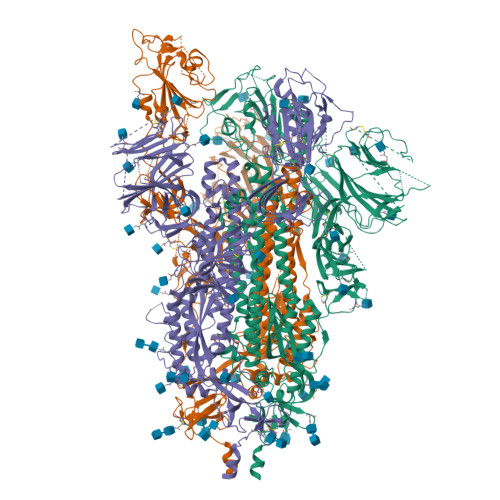
\includegraphics[width=\textwidth]{figures/shape_6vyb.jpeg}
    \caption{6VYB}
    \label{fig:shape-6vyb}
\end{subfigure}
\hfill
\begin{subfigure}[b]{0.47\textwidth}
    \centering
    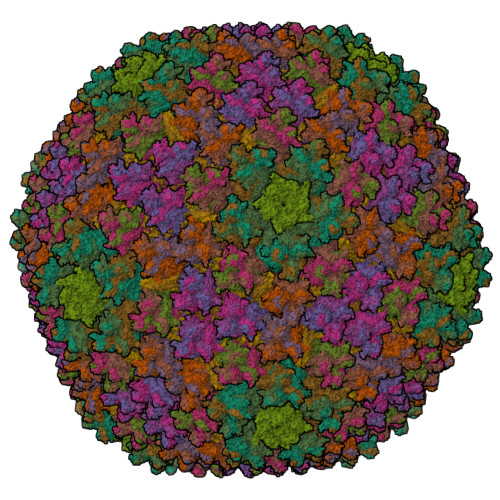
\includegraphics[width=\textwidth]{figures/shape_1vsz.jpeg}
    \caption{6CGV}
    \label{fig:shape-1vsz}
\end{subfigure}
\caption[Molecular shapes of 6VYB and 1VSZ]{Cartoon renderings of the biological assemblies, colored by chain. \textbf{Left:} 6VYB's irregular, elongated spike trimer. \textbf{Right:} the icosahedral capsid of 1VSZ, shown via its current PDB entry 6CGV, since 1VSZ itself is obsolete. Renderings from the RCSB PDB.}
\label{fig:molecule-shapes}
\end{figure}

%  Needs \usepackage{graphicx} and \usepackage{subcaption}.
% ------------------------------------------------------------------------
\begin{figure}[!htb]
\centering
\begin{subfigure}[b]{0.47\textwidth}
    \centering
    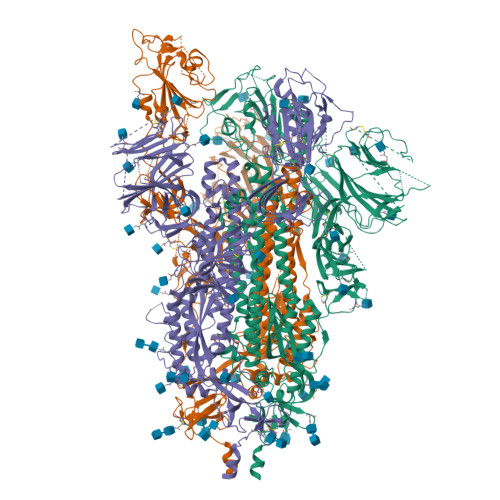
\includegraphics[width=\textwidth]{figures/shape_6vyb.jpeg}
    \caption{6VYB}
    \label{fig:shape-6vyb}
\end{subfigure}
\hfill
\begin{subfigure}[b]{0.47\textwidth}
    \centering
    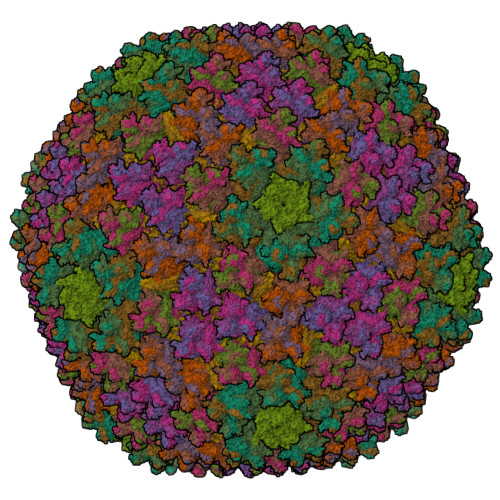
\includegraphics[width=\textwidth]{figures/shape_1vsz.jpeg}
    \caption{6CGV}
    \label{fig:shape-1vsz}
\end{subfigure}
\caption[Molecular shapes of 6VYB and 1VSZ]{Cartoon renderings of the biological assemblies, colored by chain. \textbf{Left:} 6VYB's irregular, elongated spike trimer. \textbf{Right:} the icosahedral capsid of 1VSZ, shown via its current PDB entry 6CGV, since 1VSZ itself is obsolete. Renderings from the RCSB PDB.}
\label{fig:molecule-shapes}
\end{figure}

%  Needs \usepackage{graphicx} and \usepackage{subcaption}.
% ------------------------------------------------------------------------
\begin{figure}[!htb]
\centering
\begin{subfigure}[b]{0.47\textwidth}
    \centering
    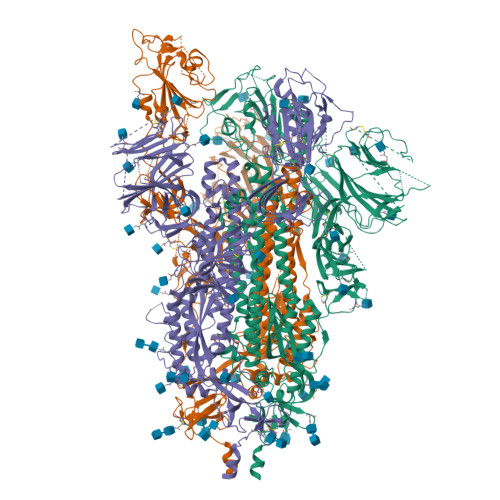
\includegraphics[width=\textwidth]{figures/shape_6vyb.jpeg}
    \caption{6VYB}
    \label{fig:shape-6vyb}
\end{subfigure}
\hfill
\begin{subfigure}[b]{0.47\textwidth}
    \centering
    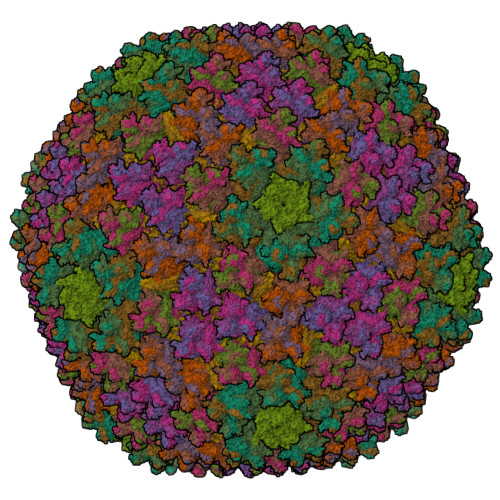
\includegraphics[width=\textwidth]{figures/shape_1vsz.jpeg}
    \caption{6CGV}
    \label{fig:shape-1vsz}
\end{subfigure}
\caption[Molecular shapes of 6VYB and 1VSZ]{Cartoon renderings of the biological assemblies, colored by chain. \textbf{Left:} 6VYB's irregular, elongated spike trimer. \textbf{Right:} the icosahedral capsid of 1VSZ, shown via its current PDB entry 6CGV, since 1VSZ itself is obsolete. Renderings from the RCSB PDB.}
\label{fig:molecule-shapes}
\end{figure}


The number of iterations are shown on top of the columns, as well as in the Table~\ref{tab:solver-bench}. 
Even though the default ``CG-Jacobi-Block'' needs consistently a lot more iterations than both LIS and the tuned configuration (in cases of 6VYB and 1VSZ 10x as many than tuned), it was still much quicker than LIS, and only marginally slower than the tuned configuration.
This demonstrates that having very cheap iterations can compensate their amount.

\subsubsection{Cluster}

Next I wanted to showcase a similar comparison for the cluster environment.
Figure~\ref{fig:solver-bench-cluster} shows the stage runtimes for 6VYB, 1VSZ and H1N1.
The former ran on a single A100 node, while H1N1 ran on the quad H200 node.
The trend does not change from the local machine, with the tuned AMGX configuration still taking the crown.
The timing breakdown can be seen in Table~\ref{tab:solver-bench-cluster}.
Surprisingly the ``slower'' A100-node's CPU managed to run LIS faster the local CPU, probably due to running with 16 ranks instead of 4.
On the other hand, the host time on the AMGX path was around 500 milliseconds longer.
This might suggest that a higher rank count makes the host work more expensive, but this is not the case as I will demonstrate shortly.
Looking at the H1N1 timings, the number of ranks does not seem to be the only factor contributing to the host time, as the stage spent almost 33 of the 42 seconds on the host.
The actual solve time meanwhile was just 3.6 seconds, with a 5.6 second setup time.
I unfortunately do not enough data to determine whether this is due my rank-gathering or if it is due to something else.
Nevertheless this would have warranted a follow-up investigation.

% ------------------------------------------------------------------------
%  Linear solver comparison (bench_sweep.py sweep A).
%  Generated by scripts/plot_solver_bench.py -- regenerate rather than edit.
%  Include with % ------------------------------------------------------------------------
%  Linear solver comparison (bench_sweep.py sweep A).
%  Generated by scripts/plot_solver_bench.py -- regenerate rather than edit.
%  Include with % ------------------------------------------------------------------------
%  Linear solver comparison (bench_sweep.py sweep A).
%  Generated by scripts/plot_solver_bench.py -- regenerate rather than edit.
%  Include with \input{figures/solver_bench_cluster}
%  Needs \usepackage{pgfplots} in the preamble.
% ------------------------------------------------------------------------
\input{figures/data/solver_bench_cluster_ref}

\pgfplotsset{compat=1.16}

% Keep only the rows whose column #1 equals #2.
\pgfplotsset{
  discard if not/.style 2 args={
    x filter/.code={%
      \edef\tempa{\thisrow{#1}}\edef\tempb{#2}%
      \ifx\tempa\tempb\else\def\pgfmathresult{inf}\fi
    }
  }
}

\definecolor{solverlis}{HTML}{D95F02}
\definecolor{solveramgx}{HTML}{9DC3E0}
\definecolor{solvercfg}{HTML}{2C5F8D}

\begin{figure}[!htb]
\centering
\begin{tikzpicture}
\begin{axis}[
    ybar,
    % The iteration-count label sits above the top whisker by 5pt, which
    % ymax's headroom does not always cover -- clip=false stops that label from
    % being cut off instead of chasing a headroom multiplier that varies with
    % how many digits the label has.
    clip=false,
    width=13.1cm, height=6.4cm,
    bar width=10pt,
    enlarge x limits=0.28,
    ymode=log, log origin y=infty,
    ymin=0.759405, ymax=17.3883,
    ytick={1,2,5,10},
    log ticks with fixed point,
    ylabel={\solverMetricsolverbenchcluster{} time, relative to the fastest},
    ylabel style={font=\footnotesize},
    symbolic x coords={6VYB,1VSZ,H1N1},
    xtick=data,
    xticklabel style={font=\footnotesize, align=center},
    tick label style={font=\scriptsize},
    ymajorgrids=true,
    major grid style={black!12},
    legend style={
      at={(0.5,-0.16)}, anchor=north, draw=none,
      legend columns=3, font=\footnotesize, column sep=0.8em,
    },
    % Run-to-run spread is only a few percent, so the upper whisker is 1-2 mm and
    % the lower half is buried in the bar fill. Caps nearly as wide as the bar
    % are what make it read as an error bar rather than a stray tick.
    % T-caps. rotate=90 is required: pgfplots draws the cap perpendicular to the
    % error direction by itself, but any mark size given here clobbers that, and
    % the cap then renders vertically -- which reads as a longer whisker rather
    % than a wider cap. Setting error mark explicitly does not help; the rotation
    % is what matters.
    error bars/error bar style={black!85, line width=0.8pt},
    error bars/error mark options={
      mark size=2.5pt, rotate=90, line width=0.8pt, black!85,
    },
    every node near coord/.append style={
      font=\tiny, color=black!60, anchor=south, yshift=5pt,
    },
]
  \addplot+[
    ybar, fill=solverlis, draw=solverlis!70!black, line width=0.4pt,
    nodes near coords, point meta=explicit symbolic,
    error bars/.cd, y dir=both, y explicit,
  ] table[x=molecule, y=lis, y error minus=lis_em, y error plus=lis_ep,
          meta=lis_it] {figures/data/solver_bench_cluster.dat};
  \addlegendentry{LIS}
  \addplot+[
    ybar, fill=solveramgx, draw=solveramgx!70!black, line width=0.4pt,
    nodes near coords, point meta=explicit symbolic,
    error bars/.cd, y dir=both, y explicit,
  ] table[x=molecule, y=amgx, y error minus=amgx_em, y error plus=amgx_ep,
          meta=amgx_it] {figures/data/solver_bench_cluster.dat};
  \addlegendentry{AMGX (default)}
  \addplot+[
    ybar, fill=solvercfg, draw=solvercfg!70!black, line width=0.4pt,
    nodes near coords, point meta=explicit symbolic,
    error bars/.cd, y dir=both, y explicit,
  ] table[x=molecule, y=amgxcfg, y error minus=amgxcfg_em, y error plus=amgxcfg_ep,
          meta=amgxcfg_it] {figures/data/solver_bench_cluster.dat};
  \addlegendentry{AMGX (tuned)}

\end{axis}
\end{tikzpicture}

\caption[Linear solver comparison]{\textbf{Linear solver comparison on
    \solverMoleculessolverbenchcluster{}.} Median \solverMetricsolverbenchcluster{} time over \solverRepeatssolverbenchcluster{} runs on a logarithmic axis,
    whiskers spanning fastest to slowest; the figure above each column is the
    iteration count.\solverMachinesolverbenchcluster{}\solverCaveatssolverbenchcluster{}}
\label{fig:solver-bench-cluster}
\end{figure}

%  Needs \usepackage{pgfplots} in the preamble.
% ------------------------------------------------------------------------
% generated by scripts/plot_solver_bench.py -- do not edit
\def\solverMetricsolverbenchcluster{solve stage}
\def\solverRepeatssolverbenchcluster{3}
\def\solverUnitsolverbenchcluster{relative to the fastest}
\def\solverMoleculessolverbenchcluster{6VYB, 1VSZ, H1N1}
\def\solverEnergyMethodsolverbenchcluster{1}
\def\solverMachinesolverbenchcluster{ Measured on an A100 node of the TU Berlin HPC (Table~\ref{tab:test-systems}) with 16 MPI ranks.}
\def\solverCaveatssolverbenchcluster{ H1N1: measured on four H200 GPUs of the TU Berlin HPC (Table~\ref{tab:test-systems}) with 8 MPI ranks; 1 run per configuration, not 3.}


\pgfplotsset{compat=1.16}

% Keep only the rows whose column #1 equals #2.
\pgfplotsset{
  discard if not/.style 2 args={
    x filter/.code={%
      \edef\tempa{\thisrow{#1}}\edef\tempb{#2}%
      \ifx\tempa\tempb\else\def\pgfmathresult{inf}\fi
    }
  }
}

\definecolor{solverlis}{HTML}{D95F02}
\definecolor{solveramgx}{HTML}{9DC3E0}
\definecolor{solvercfg}{HTML}{2C5F8D}

\begin{figure}[!htb]
\centering
\begin{tikzpicture}
\begin{axis}[
    ybar,
    % The iteration-count label sits above the top whisker by 5pt, which
    % ymax's headroom does not always cover -- clip=false stops that label from
    % being cut off instead of chasing a headroom multiplier that varies with
    % how many digits the label has.
    clip=false,
    width=13.1cm, height=6.4cm,
    bar width=10pt,
    enlarge x limits=0.28,
    ymode=log, log origin y=infty,
    ymin=0.759405, ymax=17.3883,
    ytick={1,2,5,10},
    log ticks with fixed point,
    ylabel={\solverMetricsolverbenchcluster{} time, relative to the fastest},
    ylabel style={font=\footnotesize},
    symbolic x coords={6VYB,1VSZ,H1N1},
    xtick=data,
    xticklabel style={font=\footnotesize, align=center},
    tick label style={font=\scriptsize},
    ymajorgrids=true,
    major grid style={black!12},
    legend style={
      at={(0.5,-0.16)}, anchor=north, draw=none,
      legend columns=3, font=\footnotesize, column sep=0.8em,
    },
    % Run-to-run spread is only a few percent, so the upper whisker is 1-2 mm and
    % the lower half is buried in the bar fill. Caps nearly as wide as the bar
    % are what make it read as an error bar rather than a stray tick.
    % T-caps. rotate=90 is required: pgfplots draws the cap perpendicular to the
    % error direction by itself, but any mark size given here clobbers that, and
    % the cap then renders vertically -- which reads as a longer whisker rather
    % than a wider cap. Setting error mark explicitly does not help; the rotation
    % is what matters.
    error bars/error bar style={black!85, line width=0.8pt},
    error bars/error mark options={
      mark size=2.5pt, rotate=90, line width=0.8pt, black!85,
    },
    every node near coord/.append style={
      font=\tiny, color=black!60, anchor=south, yshift=5pt,
    },
]
  \addplot+[
    ybar, fill=solverlis, draw=solverlis!70!black, line width=0.4pt,
    nodes near coords, point meta=explicit symbolic,
    error bars/.cd, y dir=both, y explicit,
  ] table[x=molecule, y=lis, y error minus=lis_em, y error plus=lis_ep,
          meta=lis_it] {figures/data/solver_bench_cluster.dat};
  \addlegendentry{LIS}
  \addplot+[
    ybar, fill=solveramgx, draw=solveramgx!70!black, line width=0.4pt,
    nodes near coords, point meta=explicit symbolic,
    error bars/.cd, y dir=both, y explicit,
  ] table[x=molecule, y=amgx, y error minus=amgx_em, y error plus=amgx_ep,
          meta=amgx_it] {figures/data/solver_bench_cluster.dat};
  \addlegendentry{AMGX (default)}
  \addplot+[
    ybar, fill=solvercfg, draw=solvercfg!70!black, line width=0.4pt,
    nodes near coords, point meta=explicit symbolic,
    error bars/.cd, y dir=both, y explicit,
  ] table[x=molecule, y=amgxcfg, y error minus=amgxcfg_em, y error plus=amgxcfg_ep,
          meta=amgxcfg_it] {figures/data/solver_bench_cluster.dat};
  \addlegendentry{AMGX (tuned)}

\end{axis}
\end{tikzpicture}

\caption[Linear solver comparison]{\textbf{Linear solver comparison on
    \solverMoleculessolverbenchcluster{}.} Median \solverMetricsolverbenchcluster{} time over \solverRepeatssolverbenchcluster{} runs on a logarithmic axis,
    whiskers spanning fastest to slowest; the figure above each column is the
    iteration count.\solverMachinesolverbenchcluster{}\solverCaveatssolverbenchcluster{}}
\label{fig:solver-bench-cluster}
\end{figure}

%  Needs \usepackage{pgfplots} in the preamble.
% ------------------------------------------------------------------------
% generated by scripts/plot_solver_bench.py -- do not edit
\def\solverMetricsolverbenchcluster{solve stage}
\def\solverRepeatssolverbenchcluster{3}
\def\solverUnitsolverbenchcluster{relative to the fastest}
\def\solverMoleculessolverbenchcluster{6VYB, 1VSZ, H1N1}
\def\solverEnergyMethodsolverbenchcluster{1}
\def\solverMachinesolverbenchcluster{ Measured on an A100 node of the TU Berlin HPC (Table~\ref{tab:test-systems}) with 16 MPI ranks.}
\def\solverCaveatssolverbenchcluster{ H1N1: measured on four H200 GPUs of the TU Berlin HPC (Table~\ref{tab:test-systems}) with 8 MPI ranks; 1 run per configuration, not 3.}


\pgfplotsset{compat=1.16}

% Keep only the rows whose column #1 equals #2.
\pgfplotsset{
  discard if not/.style 2 args={
    x filter/.code={%
      \edef\tempa{\thisrow{#1}}\edef\tempb{#2}%
      \ifx\tempa\tempb\else\def\pgfmathresult{inf}\fi
    }
  }
}

\definecolor{solverlis}{HTML}{D95F02}
\definecolor{solveramgx}{HTML}{9DC3E0}
\definecolor{solvercfg}{HTML}{2C5F8D}

\begin{figure}[!htb]
\centering
\begin{tikzpicture}
\begin{axis}[
    ybar,
    % The iteration-count label sits above the top whisker by 5pt, which
    % ymax's headroom does not always cover -- clip=false stops that label from
    % being cut off instead of chasing a headroom multiplier that varies with
    % how many digits the label has.
    clip=false,
    width=13.1cm, height=6.4cm,
    bar width=10pt,
    enlarge x limits=0.28,
    ymode=log, log origin y=infty,
    ymin=0.759405, ymax=17.3883,
    ytick={1,2,5,10},
    log ticks with fixed point,
    ylabel={\solverMetricsolverbenchcluster{} time, relative to the fastest},
    ylabel style={font=\footnotesize},
    symbolic x coords={6VYB,1VSZ,H1N1},
    xtick=data,
    xticklabel style={font=\footnotesize, align=center},
    tick label style={font=\scriptsize},
    ymajorgrids=true,
    major grid style={black!12},
    legend style={
      at={(0.5,-0.16)}, anchor=north, draw=none,
      legend columns=3, font=\footnotesize, column sep=0.8em,
    },
    % Run-to-run spread is only a few percent, so the upper whisker is 1-2 mm and
    % the lower half is buried in the bar fill. Caps nearly as wide as the bar
    % are what make it read as an error bar rather than a stray tick.
    % T-caps. rotate=90 is required: pgfplots draws the cap perpendicular to the
    % error direction by itself, but any mark size given here clobbers that, and
    % the cap then renders vertically -- which reads as a longer whisker rather
    % than a wider cap. Setting error mark explicitly does not help; the rotation
    % is what matters.
    error bars/error bar style={black!85, line width=0.8pt},
    error bars/error mark options={
      mark size=2.5pt, rotate=90, line width=0.8pt, black!85,
    },
    every node near coord/.append style={
      font=\tiny, color=black!60, anchor=south, yshift=5pt,
    },
]
  \addplot+[
    ybar, fill=solverlis, draw=solverlis!70!black, line width=0.4pt,
    nodes near coords, point meta=explicit symbolic,
    error bars/.cd, y dir=both, y explicit,
  ] table[x=molecule, y=lis, y error minus=lis_em, y error plus=lis_ep,
          meta=lis_it] {figures/data/solver_bench_cluster.dat};
  \addlegendentry{LIS}
  \addplot+[
    ybar, fill=solveramgx, draw=solveramgx!70!black, line width=0.4pt,
    nodes near coords, point meta=explicit symbolic,
    error bars/.cd, y dir=both, y explicit,
  ] table[x=molecule, y=amgx, y error minus=amgx_em, y error plus=amgx_ep,
          meta=amgx_it] {figures/data/solver_bench_cluster.dat};
  \addlegendentry{AMGX (default)}
  \addplot+[
    ybar, fill=solvercfg, draw=solvercfg!70!black, line width=0.4pt,
    nodes near coords, point meta=explicit symbolic,
    error bars/.cd, y dir=both, y explicit,
  ] table[x=molecule, y=amgxcfg, y error minus=amgxcfg_em, y error plus=amgxcfg_ep,
          meta=amgxcfg_it] {figures/data/solver_bench_cluster.dat};
  \addlegendentry{AMGX (tuned)}

\end{axis}
\end{tikzpicture}

\caption[Linear solver comparison]{\textbf{Linear solver comparison on
    \solverMoleculessolverbenchcluster{}.} Median \solverMetricsolverbenchcluster{} time over \solverRepeatssolverbenchcluster{} runs on a logarithmic axis,
    whiskers spanning fastest to slowest; the figure above each column is the
    iteration count.\solverMachinesolverbenchcluster{}\solverCaveatssolverbenchcluster{}}
\label{fig:solver-bench-cluster}
\end{figure}

% generated by scripts/plot_solver_bench.py -- do not edit
\begin{table}[!htb]
\centering
\footnotesize
\caption[Linear solver comparison]{\textbf{Linear solver comparison.} Median over \solverRepeatssolverbenchcluster{} runs. \emph{stage} is the whole \solverMetricsolverbenchcluster{}, split into the part AMGX spends on the GPU (its own \emph{setup} and \emph{solve} timers) and the \emph{host} remainder -- assembly, host--device transfer and the surrounding CPU work, which no faster accelerator touches and which can dominate the total. \emph{rel.} is the stage time relative to the fastest configuration for that molecule. LIS never touches the GPU, so its whole stage is host time.\solverMachinesolverbenchcluster{}\solverCaveatssolverbenchcluster{} The residuals differ by orders of magnitude, so the times are not like-for-like.}
\label{tab:solver-bench-cluster}
\begin{tabular}{llrrrrrrl}
\toprule
& & & \multicolumn{2}{c}{GPU [s]} & & & & \\
\cmidrule(lr){4-5}
molecule & configuration & iters & setup & solve & host [s] & stage [s] & rel. & residual \\
\midrule
6VYB & LIS & 188 & -- & -- & 46.0255 & 46.0255 & 8.47$\times$ & $3.7\times10^{-7}$ \\
 & AMGX (default) & 527 & 0.0194 & 2.8597 & 4.3105 & 7.1897 & 1.32$\times$ & $4.3\times10^{-8}$ \\
 & AMGX (tuned) & 51 & 0.2097 & 0.9270 & 4.2947 & 5.4315 & 1.00$\times$ & $3.2\times10^{-8}$ \\
\midrule
1VSZ & LIS & 164 & -- & -- & 24.4038 & 24.4038 & 6.99$\times$ & $8.9\times10^{-7}$ \\
 & AMGX (default) & 523 & 0.0037 & 1.6543 & 2.8241 & 4.4821 & 1.28$\times$ & $2.7\times10^{-8}$ \\
 & AMGX (tuned) & 51 & 0.1702 & 0.5495 & 2.7697 & 3.4894 & 1.00$\times$ & $2.1\times10^{-8}$ \\
\midrule
H1N1 & LIS & 169 & -- & -- & 518.3410 & 518.3410 & 12.30$\times$ & $3.5\times10^{-7}$ \\
 & AMGX (tuned) & 31 & 5.5863 & 3.5901 & 32.9625 & 42.1390 & 1.00$\times$ & $4.9\times10^{-7}$ \\
\bottomrule
\end{tabular}
\end{table}


\subsubsection{Scaling Across Topologies}

I then compared the AMGX solve time for 6VYB for four different topologies: the local system, a one cluster node with a single A100 GPU, one with dual A100 GPUs and two nodes with one A100 each, shown in Figure~\ref{fig:amgx_scaling_6vyb}.
The goal was to see how well AMGX scales across multiple nodes, and GPUs.
To compare the single cluster node to the local system, I also included 4-rank runs on the cluster to match the local runs.
Comparing the local system to a single cluster node with one A100 GPU launched with 4 ranks, the actual solve time decreased by over 2x.
Despite this the overall stage time in case of the tuned AMGX configuration increased.
This is again, due to the weak cluster CPU, which slows down the host portion of the linear solve from 3.8 seconds to 5.45 seconds, as can be seen in the timing breakdown in Table~\ref{tab:amgx_scaling_6vyb}.
Increasing the number of ranks to 16 reduces the host time, disproving that a higher rank count make the host time more expensive.
Instead it suggests that a significant contributor to the host time might not be the gathering after all.

The Figure~\ref{fig:amgx_scaling_6vyb} also shows that AMGX scales much better across multiple GPUs per node, but not on multiple nodes.
The tuned configuration performed significantly worse on two nodes than it did on a single node.
This is very likely due to communication overhead, which is much lower on a single node with multiple GPUs as I showed in \ref{tab:test-systems}.
There the tuned AMGX performed much better than the single GPU node.
Surprisingly, the default configuration did not suffer as much, although it was barely any faster than one single GPU node.
This suggests that AMG preconditioning is more communication-intensive than even a multitude of cheap iterations.
Despite this, the pure solve time of the tuned AMGX config was still faster on two nodes than the default configuration, as was the full stage time.

% ------------------------------------------------------------------------
%  AMGX scaling across GPUs and topologies.
%  Generated by scripts/plot_amgx_scaling.py -- regenerate rather than edit.
%  Include with % ------------------------------------------------------------------------
%  AMGX scaling across GPUs and topologies.
%  Generated by scripts/plot_amgx_scaling.py -- regenerate rather than edit.
%  Include with % ------------------------------------------------------------------------
%  AMGX scaling across GPUs and topologies.
%  Generated by scripts/plot_amgx_scaling.py -- regenerate rather than edit.
%  Include with \input{figures/amgx_scaling_6vyb}
%  Needs \usepackage{pgfplots} in the preamble.
% ------------------------------------------------------------------------
\input{figures/data/amgx_scaling_6vyb_ref}

\pgfplotsset{compat=1.16}
\usepgfplotslibrary{groupplots}

\definecolor{amgxsetup}{HTML}{9DC3E0}
\definecolor{amgxsolve}{HTML}{2C5F8D}

\begin{figure}[!htb]
\centering
\begin{tikzpicture}
\begin{groupplot}[
    group style={
      group size=2 by 1,
      horizontal sep=1.5cm,
    },
    width=7.4cm, height=6.2cm,
    enlarge x limits=0.14,
    ymin=0,
    ylabel={AMGX time [s]},
    ylabel style={font=\footnotesize},
    symbolic x coords={s0,s1,s2,s3,s4},
    xtick=data,
    xticklabels={{RTX 3080\\1 GPU\\4 ranks}, {A100\\1 GPU\\4 ranks}, {A100\\1 GPU\\16 ranks}, {A100\\2 GPUs\\1 node}, {A100\\2 GPUs\\2 nodes}},
    xticklabel style={font=\tiny, align=center, yshift=-0.2ex},
    tick label style={font=\scriptsize},
    title style={font=\footnotesize, yshift=-0.4ex},
    ymajorgrids=true,
    major grid style={black!12},
]

\nextgroupplot[ybar stacked, bar width=13pt, title={tuned: \texttt{amgx\_pcgf\_amg\_block\_jacobi}}, ymax=2.77813, legend style={draw=none, font=\footnotesize, column sep=0.8em}, legend columns=2, legend to name=amgxlegendamgxscalingvyb]
  \addplot[fill=amgxsetup, draw=amgxsetup!70!black, line width=0.4pt]
    table[x=sx, y=setup] {figures/data/amgx_scaling_6vyb_c0.dat};
  \addlegendentry{setup}
  \addplot[fill=amgxsolve, draw=amgxsolve!70!black, line width=0.4pt]
    table[x=sx, y=solve] {figures/data/amgx_scaling_6vyb_c0.dat};
  \addlegendentry{solve}
  % Explicit nodes rather than `nodes near coords`: inside `ybar stacked` the
  % latter anchors each label at its own segment's height, i.e. partway up the
  % bar, and `stack plots=false` on an overlay plot earns a bar shift instead.
  % The totals are known here, so the placement can just be stated.
  \node[font=\tiny, text=black!55, anchor=south, yshift=1pt] at (axis cs:s0,2.39494) {$\times$0.47};
  \node[font=\tiny, text=black!55, anchor=south, yshift=1pt] at (axis cs:s1,1.0932) {$\times$1.04};
  \node[font=\tiny, text=black!55, anchor=south, yshift=1pt] at (axis cs:s2,1.13158) {$\times$1.00};
  \node[font=\tiny, text=black!55, anchor=south, yshift=1pt] at (axis cs:s3,0.7142) {$\times$1.58};
  \node[font=\tiny, text=black!55, anchor=south, yshift=1pt] at (axis cs:s4,1.83034) {$\times$0.62};

\nextgroupplot[ybar stacked, bar width=13pt, title={AMGX default}, ymax=7.50473, legend style={draw=none}]
  \addplot[fill=amgxsetup, draw=amgxsetup!70!black, line width=0.4pt]
    table[x=sx, y=setup] {figures/data/amgx_scaling_6vyb_c1.dat};
  
  \addplot[fill=amgxsolve, draw=amgxsolve!70!black, line width=0.4pt]
    table[x=sx, y=solve] {figures/data/amgx_scaling_6vyb_c1.dat};
  
  % Explicit nodes rather than `nodes near coords`: inside `ybar stacked` the
  % latter anchors each label at its own segment's height, i.e. partway up the
  % bar, and `stack plots=false` on an overlay plot earns a bar shift instead.
  % The totals are known here, so the placement can just be stated.
  \node[font=\tiny, text=black!55, anchor=south, yshift=1pt] at (axis cs:s0,6.46959) {$\times$0.44};
  \node[font=\tiny, text=black!55, anchor=south, yshift=1pt] at (axis cs:s1,2.87817) {$\times$1.00};
  \node[font=\tiny, text=black!55, anchor=south, yshift=1pt] at (axis cs:s2,2.87054) {$\times$1.00};
  \node[font=\tiny, text=black!55, anchor=south, yshift=1pt] at (axis cs:s3,1.6726) {$\times$1.72};
  \node[font=\tiny, text=black!55, anchor=south, yshift=1pt] at (axis cs:s4,2.71847) {$\times$1.06};

\end{groupplot}
\end{tikzpicture}

\vspace{0.4ex}
\ref{amgxlegendamgxscalingvyb}

\caption[AMGX scaling across GPUs and topologies]{\textbf{AMGX setup and solve
    time on \amgxMoleculeamgxscalingvyb{} over five GPU configurations.} Median over at least
    \amgxRepeatsamgxscalingvyb{} runs per bar, from AMGX's own timers. The figure above each
    bar is its total relative to \amgxRefamgxscalingvyb{}. \emph{Left:} the tuned
    configuration \amgxTunedNameamgxscalingvyb{}, \amgxTunedItersamgxscalingvyb{} iterations.
    \emph{Right:} AMGX's default, \amgxDefaultItersamgxscalingvyb{} iterations, on its own
    $y$ scale.}
\label{fig:amgx_scaling_6vyb}
\end{figure}

%  Needs \usepackage{pgfplots} in the preamble.
% ------------------------------------------------------------------------
% generated by scripts/plot_amgx_scaling.py -- do not edit
\def\amgxMoleculeamgxscalingvyb{6VYB}
\def\amgxRefamgxscalingvyb{A100, 1 GPU, 16 ranks}
\def\amgxRepeatsamgxscalingvyb{3}
\def\amgxTunedNameamgxscalingvyb{\texttt{amgx\_pcgf\_amg\_block\_jacobi}}
\def\amgxTunedItersamgxscalingvyb{51}
\def\amgxDefaultItersamgxscalingvyb{527}


\pgfplotsset{compat=1.16}
\usepgfplotslibrary{groupplots}

\definecolor{amgxsetup}{HTML}{9DC3E0}
\definecolor{amgxsolve}{HTML}{2C5F8D}

\begin{figure}[!htb]
\centering
\begin{tikzpicture}
\begin{groupplot}[
    group style={
      group size=2 by 1,
      horizontal sep=1.5cm,
    },
    width=7.4cm, height=6.2cm,
    enlarge x limits=0.14,
    ymin=0,
    ylabel={AMGX time [s]},
    ylabel style={font=\footnotesize},
    symbolic x coords={s0,s1,s2,s3,s4},
    xtick=data,
    xticklabels={{RTX 3080\\1 GPU\\4 ranks}, {A100\\1 GPU\\4 ranks}, {A100\\1 GPU\\16 ranks}, {A100\\2 GPUs\\1 node}, {A100\\2 GPUs\\2 nodes}},
    xticklabel style={font=\tiny, align=center, yshift=-0.2ex},
    tick label style={font=\scriptsize},
    title style={font=\footnotesize, yshift=-0.4ex},
    ymajorgrids=true,
    major grid style={black!12},
]

\nextgroupplot[ybar stacked, bar width=13pt, title={tuned: \texttt{amgx\_pcgf\_amg\_block\_jacobi}}, ymax=2.77813, legend style={draw=none, font=\footnotesize, column sep=0.8em}, legend columns=2, legend to name=amgxlegendamgxscalingvyb]
  \addplot[fill=amgxsetup, draw=amgxsetup!70!black, line width=0.4pt]
    table[x=sx, y=setup] {figures/data/amgx_scaling_6vyb_c0.dat};
  \addlegendentry{setup}
  \addplot[fill=amgxsolve, draw=amgxsolve!70!black, line width=0.4pt]
    table[x=sx, y=solve] {figures/data/amgx_scaling_6vyb_c0.dat};
  \addlegendentry{solve}
  % Explicit nodes rather than `nodes near coords`: inside `ybar stacked` the
  % latter anchors each label at its own segment's height, i.e. partway up the
  % bar, and `stack plots=false` on an overlay plot earns a bar shift instead.
  % The totals are known here, so the placement can just be stated.
  \node[font=\tiny, text=black!55, anchor=south, yshift=1pt] at (axis cs:s0,2.39494) {$\times$0.47};
  \node[font=\tiny, text=black!55, anchor=south, yshift=1pt] at (axis cs:s1,1.0932) {$\times$1.04};
  \node[font=\tiny, text=black!55, anchor=south, yshift=1pt] at (axis cs:s2,1.13158) {$\times$1.00};
  \node[font=\tiny, text=black!55, anchor=south, yshift=1pt] at (axis cs:s3,0.7142) {$\times$1.58};
  \node[font=\tiny, text=black!55, anchor=south, yshift=1pt] at (axis cs:s4,1.83034) {$\times$0.62};

\nextgroupplot[ybar stacked, bar width=13pt, title={AMGX default}, ymax=7.50473, legend style={draw=none}]
  \addplot[fill=amgxsetup, draw=amgxsetup!70!black, line width=0.4pt]
    table[x=sx, y=setup] {figures/data/amgx_scaling_6vyb_c1.dat};
  
  \addplot[fill=amgxsolve, draw=amgxsolve!70!black, line width=0.4pt]
    table[x=sx, y=solve] {figures/data/amgx_scaling_6vyb_c1.dat};
  
  % Explicit nodes rather than `nodes near coords`: inside `ybar stacked` the
  % latter anchors each label at its own segment's height, i.e. partway up the
  % bar, and `stack plots=false` on an overlay plot earns a bar shift instead.
  % The totals are known here, so the placement can just be stated.
  \node[font=\tiny, text=black!55, anchor=south, yshift=1pt] at (axis cs:s0,6.46959) {$\times$0.44};
  \node[font=\tiny, text=black!55, anchor=south, yshift=1pt] at (axis cs:s1,2.87817) {$\times$1.00};
  \node[font=\tiny, text=black!55, anchor=south, yshift=1pt] at (axis cs:s2,2.87054) {$\times$1.00};
  \node[font=\tiny, text=black!55, anchor=south, yshift=1pt] at (axis cs:s3,1.6726) {$\times$1.72};
  \node[font=\tiny, text=black!55, anchor=south, yshift=1pt] at (axis cs:s4,2.71847) {$\times$1.06};

\end{groupplot}
\end{tikzpicture}

\vspace{0.4ex}
\ref{amgxlegendamgxscalingvyb}

\caption[AMGX scaling across GPUs and topologies]{\textbf{AMGX setup and solve
    time on \amgxMoleculeamgxscalingvyb{} over five GPU configurations.} Median over at least
    \amgxRepeatsamgxscalingvyb{} runs per bar, from AMGX's own timers. The figure above each
    bar is its total relative to \amgxRefamgxscalingvyb{}. \emph{Left:} the tuned
    configuration \amgxTunedNameamgxscalingvyb{}, \amgxTunedItersamgxscalingvyb{} iterations.
    \emph{Right:} AMGX's default, \amgxDefaultItersamgxscalingvyb{} iterations, on its own
    $y$ scale.}
\label{fig:amgx_scaling_6vyb}
\end{figure}

%  Needs \usepackage{pgfplots} in the preamble.
% ------------------------------------------------------------------------
% generated by scripts/plot_amgx_scaling.py -- do not edit
\def\amgxMoleculeamgxscalingvyb{6VYB}
\def\amgxRefamgxscalingvyb{A100, 1 GPU, 16 ranks}
\def\amgxRepeatsamgxscalingvyb{3}
\def\amgxTunedNameamgxscalingvyb{\texttt{amgx\_pcgf\_amg\_block\_jacobi}}
\def\amgxTunedItersamgxscalingvyb{51}
\def\amgxDefaultItersamgxscalingvyb{527}


\pgfplotsset{compat=1.16}
\usepgfplotslibrary{groupplots}

\definecolor{amgxsetup}{HTML}{9DC3E0}
\definecolor{amgxsolve}{HTML}{2C5F8D}

\begin{figure}[!htb]
\centering
\begin{tikzpicture}
\begin{groupplot}[
    group style={
      group size=2 by 1,
      horizontal sep=1.5cm,
    },
    width=7.4cm, height=6.2cm,
    enlarge x limits=0.14,
    ymin=0,
    ylabel={AMGX time [s]},
    ylabel style={font=\footnotesize},
    symbolic x coords={s0,s1,s2,s3,s4},
    xtick=data,
    xticklabels={{RTX 3080\\1 GPU\\4 ranks}, {A100\\1 GPU\\4 ranks}, {A100\\1 GPU\\16 ranks}, {A100\\2 GPUs\\1 node}, {A100\\2 GPUs\\2 nodes}},
    xticklabel style={font=\tiny, align=center, yshift=-0.2ex},
    tick label style={font=\scriptsize},
    title style={font=\footnotesize, yshift=-0.4ex},
    ymajorgrids=true,
    major grid style={black!12},
]

\nextgroupplot[ybar stacked, bar width=13pt, title={tuned: \texttt{amgx\_pcgf\_amg\_block\_jacobi}}, ymax=2.77813, legend style={draw=none, font=\footnotesize, column sep=0.8em}, legend columns=2, legend to name=amgxlegendamgxscalingvyb]
  \addplot[fill=amgxsetup, draw=amgxsetup!70!black, line width=0.4pt]
    table[x=sx, y=setup] {figures/data/amgx_scaling_6vyb_c0.dat};
  \addlegendentry{setup}
  \addplot[fill=amgxsolve, draw=amgxsolve!70!black, line width=0.4pt]
    table[x=sx, y=solve] {figures/data/amgx_scaling_6vyb_c0.dat};
  \addlegendentry{solve}
  % Explicit nodes rather than `nodes near coords`: inside `ybar stacked` the
  % latter anchors each label at its own segment's height, i.e. partway up the
  % bar, and `stack plots=false` on an overlay plot earns a bar shift instead.
  % The totals are known here, so the placement can just be stated.
  \node[font=\tiny, text=black!55, anchor=south, yshift=1pt] at (axis cs:s0,2.39494) {$\times$0.47};
  \node[font=\tiny, text=black!55, anchor=south, yshift=1pt] at (axis cs:s1,1.0932) {$\times$1.04};
  \node[font=\tiny, text=black!55, anchor=south, yshift=1pt] at (axis cs:s2,1.13158) {$\times$1.00};
  \node[font=\tiny, text=black!55, anchor=south, yshift=1pt] at (axis cs:s3,0.7142) {$\times$1.58};
  \node[font=\tiny, text=black!55, anchor=south, yshift=1pt] at (axis cs:s4,1.83034) {$\times$0.62};

\nextgroupplot[ybar stacked, bar width=13pt, title={AMGX default}, ymax=7.50473, legend style={draw=none}]
  \addplot[fill=amgxsetup, draw=amgxsetup!70!black, line width=0.4pt]
    table[x=sx, y=setup] {figures/data/amgx_scaling_6vyb_c1.dat};
  
  \addplot[fill=amgxsolve, draw=amgxsolve!70!black, line width=0.4pt]
    table[x=sx, y=solve] {figures/data/amgx_scaling_6vyb_c1.dat};
  
  % Explicit nodes rather than `nodes near coords`: inside `ybar stacked` the
  % latter anchors each label at its own segment's height, i.e. partway up the
  % bar, and `stack plots=false` on an overlay plot earns a bar shift instead.
  % The totals are known here, so the placement can just be stated.
  \node[font=\tiny, text=black!55, anchor=south, yshift=1pt] at (axis cs:s0,6.46959) {$\times$0.44};
  \node[font=\tiny, text=black!55, anchor=south, yshift=1pt] at (axis cs:s1,2.87817) {$\times$1.00};
  \node[font=\tiny, text=black!55, anchor=south, yshift=1pt] at (axis cs:s2,2.87054) {$\times$1.00};
  \node[font=\tiny, text=black!55, anchor=south, yshift=1pt] at (axis cs:s3,1.6726) {$\times$1.72};
  \node[font=\tiny, text=black!55, anchor=south, yshift=1pt] at (axis cs:s4,2.71847) {$\times$1.06};

\end{groupplot}
\end{tikzpicture}

\vspace{0.4ex}
\ref{amgxlegendamgxscalingvyb}

\caption[AMGX scaling across GPUs and topologies]{\textbf{AMGX setup and solve
    time on \amgxMoleculeamgxscalingvyb{} over five GPU configurations.} Median over at least
    \amgxRepeatsamgxscalingvyb{} runs per bar, from AMGX's own timers. The figure above each
    bar is its total relative to \amgxRefamgxscalingvyb{}. \emph{Left:} the tuned
    configuration \amgxTunedNameamgxscalingvyb{}, \amgxTunedItersamgxscalingvyb{} iterations.
    \emph{Right:} AMGX's default, \amgxDefaultItersamgxscalingvyb{} iterations, on its own
    $y$ scale.}
\label{fig:amgx_scaling_6vyb}
\end{figure}

% ------------------------------------------------------------------------
%  Generated by scripts/plot_amgx_scaling.py -- regenerate rather than edit.
%  Include with % ------------------------------------------------------------------------
%  Generated by scripts/plot_amgx_scaling.py -- regenerate rather than edit.
%  Include with % ------------------------------------------------------------------------
%  Generated by scripts/plot_amgx_scaling.py -- regenerate rather than edit.
%  Include with \input{figures/amgx_scaling_6vyb_table}
%  Needs \usepackage{booktabs}.
% ------------------------------------------------------------------------
\begin{table}[!htb]
\centering
\footnotesize
% Eight columns is 6pt over a 16cm text block at the default 6pt tabcolsep.
\setlength{\tabcolsep}{4.5pt}
\caption[AMGX scaling against the whole solve stage]{\textbf{The numbers behind
    figure~\ref{fig:amgx_scaling_6vyb}.} \emph{AMGX} is setup${}+{}$solve from AMGX's own
    timers; \emph{rest} is \texttt{t\_solve} minus that. \emph{spread} is the
    widest repeat-to-repeat variation in the row; a bracketed figure excludes
    the job's first AMGX call.}
\label{tab:amgx_scaling_6vyb}
\begin{tabular}{lrrrrrrr}
\toprule
platform & iters & setup [s] & solve [s] & AMGX [s] & vs.\ ref. & spread & rest [s] \\
\midrule
\multicolumn{8}{l}{\emph{\texttt{amgx\_pcgf\_amg\_block\_jacobi}}} \\
RTX 3080, 1 GPU, 4 ranks & 51 & 0.337 & 2.051 & 2.395 & $\times$0.47 & 10\% & 3.82 \\
A100, 1 GPU, 4 ranks & 51 & 0.174 & 0.921 & 1.093 & $\times$1.04 & 40\% (2\%) & 5.45 \\
A100, 1 GPU, 16 ranks & 51 & 0.207 & 0.924 & 1.132 & $\times$1.00 & 37\% (6\%) & 4.57 \\
A100, 2 GPUs, 1 node & 51--52 & 0.108 & 0.604 & 0.714 & $\times$1.58 & 102\% (8\%) & 4.87 \\
A100, 2 GPUs, 2 nodes & 51--52 & 0.374 & 1.454 & 1.830 & $\times$0.62 & 16\% & 4.89 \\
\midrule
\multicolumn{8}{l}{\emph{AMGX default}} \\
RTX 3080, 1 GPU, 4 ranks & 527 & 0.005 & 6.464 & 6.470 & $\times$0.44 & 4\% & 3.84 \\
A100, 1 GPU, 4 ranks & 527 & 0.021 & 2.857 & 2.878 & $\times$1.00 & 1\% & 5.37 \\
A100, 1 GPU, 16 ranks & 527 & 0.006 & 2.863 & 2.871 & $\times$1.00 & 1\% & 4.62 \\
A100, 2 GPUs, 1 node & 527 & 0.003 & 1.669 & 1.673 & $\times$1.72 & 2\% & 4.90 \\
A100, 2 GPUs, 2 nodes & 527 & 0.024 & 2.696 & 2.718 & $\times$1.06 & 22\% & 5.13 \\
\bottomrule
\end{tabular}
\end{table}

%  Needs \usepackage{booktabs}.
% ------------------------------------------------------------------------
\begin{table}[!htb]
\centering
\footnotesize
% Eight columns is 6pt over a 16cm text block at the default 6pt tabcolsep.
\setlength{\tabcolsep}{4.5pt}
\caption[AMGX scaling against the whole solve stage]{\textbf{The numbers behind
    figure~\ref{fig:amgx_scaling_6vyb}.} \emph{AMGX} is setup${}+{}$solve from AMGX's own
    timers; \emph{rest} is \texttt{t\_solve} minus that. \emph{spread} is the
    widest repeat-to-repeat variation in the row; a bracketed figure excludes
    the job's first AMGX call.}
\label{tab:amgx_scaling_6vyb}
\begin{tabular}{lrrrrrrr}
\toprule
platform & iters & setup [s] & solve [s] & AMGX [s] & vs.\ ref. & spread & rest [s] \\
\midrule
\multicolumn{8}{l}{\emph{\texttt{amgx\_pcgf\_amg\_block\_jacobi}}} \\
RTX 3080, 1 GPU, 4 ranks & 51 & 0.337 & 2.051 & 2.395 & $\times$0.47 & 10\% & 3.82 \\
A100, 1 GPU, 4 ranks & 51 & 0.174 & 0.921 & 1.093 & $\times$1.04 & 40\% (2\%) & 5.45 \\
A100, 1 GPU, 16 ranks & 51 & 0.207 & 0.924 & 1.132 & $\times$1.00 & 37\% (6\%) & 4.57 \\
A100, 2 GPUs, 1 node & 51--52 & 0.108 & 0.604 & 0.714 & $\times$1.58 & 102\% (8\%) & 4.87 \\
A100, 2 GPUs, 2 nodes & 51--52 & 0.374 & 1.454 & 1.830 & $\times$0.62 & 16\% & 4.89 \\
\midrule
\multicolumn{8}{l}{\emph{AMGX default}} \\
RTX 3080, 1 GPU, 4 ranks & 527 & 0.005 & 6.464 & 6.470 & $\times$0.44 & 4\% & 3.84 \\
A100, 1 GPU, 4 ranks & 527 & 0.021 & 2.857 & 2.878 & $\times$1.00 & 1\% & 5.37 \\
A100, 1 GPU, 16 ranks & 527 & 0.006 & 2.863 & 2.871 & $\times$1.00 & 1\% & 4.62 \\
A100, 2 GPUs, 1 node & 527 & 0.003 & 1.669 & 1.673 & $\times$1.72 & 2\% & 4.90 \\
A100, 2 GPUs, 2 nodes & 527 & 0.024 & 2.696 & 2.718 & $\times$1.06 & 22\% & 5.13 \\
\bottomrule
\end{tabular}
\end{table}

%  Needs \usepackage{booktabs}.
% ------------------------------------------------------------------------
\begin{table}[!htb]
\centering
\footnotesize
% Eight columns is 6pt over a 16cm text block at the default 6pt tabcolsep.
\setlength{\tabcolsep}{4.5pt}
\caption[AMGX scaling against the whole solve stage]{\textbf{The numbers behind
    figure~\ref{fig:amgx_scaling_6vyb}.} \emph{AMGX} is setup${}+{}$solve from AMGX's own
    timers; \emph{rest} is \texttt{t\_solve} minus that. \emph{spread} is the
    widest repeat-to-repeat variation in the row; a bracketed figure excludes
    the job's first AMGX call.}
\label{tab:amgx_scaling_6vyb}
\begin{tabular}{lrrrrrrr}
\toprule
platform & iters & setup [s] & solve [s] & AMGX [s] & vs.\ ref. & spread & rest [s] \\
\midrule
\multicolumn{8}{l}{\emph{\texttt{amgx\_pcgf\_amg\_block\_jacobi}}} \\
RTX 3080, 1 GPU, 4 ranks & 51 & 0.337 & 2.051 & 2.395 & $\times$0.47 & 10\% & 3.82 \\
A100, 1 GPU, 4 ranks & 51 & 0.174 & 0.921 & 1.093 & $\times$1.04 & 40\% (2\%) & 5.45 \\
A100, 1 GPU, 16 ranks & 51 & 0.207 & 0.924 & 1.132 & $\times$1.00 & 37\% (6\%) & 4.57 \\
A100, 2 GPUs, 1 node & 51--52 & 0.108 & 0.604 & 0.714 & $\times$1.58 & 102\% (8\%) & 4.87 \\
A100, 2 GPUs, 2 nodes & 51--52 & 0.374 & 1.454 & 1.830 & $\times$0.62 & 16\% & 4.89 \\
\midrule
\multicolumn{8}{l}{\emph{AMGX default}} \\
RTX 3080, 1 GPU, 4 ranks & 527 & 0.005 & 6.464 & 6.470 & $\times$0.44 & 4\% & 3.84 \\
A100, 1 GPU, 4 ranks & 527 & 0.021 & 2.857 & 2.878 & $\times$1.00 & 1\% & 5.37 \\
A100, 1 GPU, 16 ranks & 527 & 0.006 & 2.863 & 2.871 & $\times$1.00 & 1\% & 4.62 \\
A100, 2 GPUs, 1 node & 527 & 0.003 & 1.669 & 1.673 & $\times$1.72 & 2\% & 4.90 \\
A100, 2 GPUs, 2 nodes & 527 & 0.024 & 2.696 & 2.718 & $\times$1.06 & 22\% & 5.13 \\
\bottomrule
\end{tabular}
\end{table}

\FloatBarrier

\subsection{FMM Parameters}
\label{sec:evaluation-results-fmm-parameters}

The FMM has multiple parameters, which I needed to balance against each other to find the optimum, those being the order of the multipole expansion $P$, the MAC parameter $\theta$ and the number of particles inside one leaf $n_{leaf}$.
I made four sweeps of $P$ and $\theta$ for values between 6 to 10 and 0.2 to 0.8 for 6VYB and 1VSZ on my local machine.
FMM was slower than the naive kernel for 1CCM, no matter which configuration I used, which is why I did not consider it for the parameter choice.
This molecule consists of only 642 atoms, at which point the overhead of FMM is simply too expensive.

\subsubsection{Multipole Order and MAC}

I've plotted their speed against their relative error compared to the naive $O(N^2)$ GPU sum over the same inputs, taken from an average of 3 runs, which can be seen in Figure~\ref{fig:fmm_presplit_6vyb} and \ref{fig:fmm_presplit_1vsz}.
In those figures and in every later sweep figure, color is the multipole order $P$ and the points along each line are the MAC parameter $\theta$, rising from $0.2$ at the accurate end to $0.8$.
Grey marks the Pareto front over the whole sweep, and the dashed vertical line the naive path's own time.

% ------------------------------------------------------------------------
%
%  Regenerated with (from the repository root):
%    M='the local system (Table~\ref{tab:test-systems})'
%    K=1.246641e-10
%    python3 scripts/plot_fmm_sweep.py test1 --csv test1/fmm_sweep_6VYB_presplit.csv \
%        --tag fmm_presplit_6vyb --molecule 6VYB --natoms 44495 \
%        --kirkwood-err $K --machine "$M"
%    python3 scripts/plot_fmm_sweep.py test2 --csv test2/fmm_sweep.csv \
%        --tag fmm_presplit_1vsz --molecule 1VSZ --natoms 14299 \
%        --kirkwood-err $K --machine "$M"
%  Add --stock-csv test<N>/bench_runs.csv to print the reproducibility numbers
% ------------------------------------------------------------------------

% ------------------------------------------------------------------------
%  FMM parameter sweep: accuracy against work.
%  Generated by scripts/plot_fmm_sweep.py -- regenerate rather than edit.
%  Include with % ------------------------------------------------------------------------
%  FMM parameter sweep: accuracy against work.
%  Generated by scripts/plot_fmm_sweep.py -- regenerate rather than edit.
%  Include with % ------------------------------------------------------------------------
%  FMM parameter sweep: accuracy against work.
%  Generated by scripts/plot_fmm_sweep.py -- regenerate rather than edit.
%  Include with \input{figures/fmm_presplit_6vyb}
%  Needs \usepackage{pgfplots} in the preamble.
% ------------------------------------------------------------------------
\input{figures/data/fmm_presplit_6vyb_ref}

\pgfplotsset{compat=1.16}
\usepgfplotslibrary{groupplots}

% Keep only the rows where column #1 equals #2 AND column #3 equals #4. Lets
% every series come from the one data table instead of twenty little files.
%
% It has to test both columns in a single style: two separate one-column filters
% on the same \addplot would both define x filter/.code, and the second silently
% replaces the first.
\pgfplotsset{
  discard if not two/.style n args={4}{
    x filter/.code={%
      \edef\tempa{\thisrow{#1}}\edef\tempb{#2}%
      \edef\tempc{\thisrow{#3}}\edef\tempd{#4}%
      \ifx\tempa\tempb
        \ifx\tempc\tempd\else\def\pgfmathresult{inf}\fi
      \else\def\pgfmathresult{inf}\fi
    }
  }
}

\definecolor{fmmp6}{HTML}{1B3A6B}
\definecolor{fmmp7}{HTML}{1F77B4}
\definecolor{fmmp8}{HTML}{17A398}
\definecolor{fmmp9}{HTML}{7EA83D}
\definecolor{fmmp10}{HTML}{E8A33D}
\definecolor{fmmfront}{HTML}{9AA0A6}

\begin{figure}[!htb]
\centering
\begin{tikzpicture}
\begin{groupplot}[
    group style={
      group size=2 by 2,
      horizontal sep=0.9cm,
      vertical sep=1.0cm,
      xlabels at=edge bottom,
      ylabels at=edge left,
      xticklabels at=edge bottom,
      yticklabels at=edge left,
    },
    width=7.2cm, height=5.4cm,
    xmode=log, ymode=log,
    xlabel={energy calculation [s]},
    ylabel={relative error},
    xlabel style={font=\footnotesize},
    ylabel style={font=\footnotesize},
    tick label style={font=\scriptsize},
    title style={font=\footnotesize, yshift=-0.4ex},
    grid=both,
    major grid style={black!12},
    minor grid style={black!5},
    minor tick num=0,
    ymin=3.33333e-17, ymax=0.000232409,
    xmin=0.434589, xmax=34.3197,
    log basis x=10, log basis y=10,
    xtick={0.5,1,2,5,10,20}, xticklabels={0.5,1,2,5,10,20},
    ytick={1e-16,1e-14,1e-12,1e-10,1e-08,1e-06,0.0001},
    legend columns=7,
    legend style={draw=none, font=\footnotesize, column sep=0.6em},
]

\nextgroupplot[title={$n_{leaf,src}/n_{leaf,tgt} = 32/32$}, legend to name=fmmlegendfmmpresplit6vyb]
  % resolution floor of the comparison
  \addplot[draw=none, fill=black!7, forget plot]
    coordinates {(0.434589,3.33333e-17) (34.3197,3.33333e-17) (34.3197,\fmmNaiveErrfmmpresplitvyb) (0.434589,\fmmNaiveErrfmmpresplitvyb)}
    \closedcycle;
  % naive O(N^2) energy time
  \addplot[black!55, dashed, line width=0.8pt, forget plot]
    coordinates {(\fmmNaiveTimefmmpresplitvyb,3.33333e-17) (\fmmNaiveTimefmmpresplitvyb,0.000232409)};
  % Pareto front over the whole sweep
  \addplot[fmmfront, line width=1.6pt, forget plot]
    table[x=time, y=err] {figures/data/fmm_presplit_6vyb_pareto.dat};
  \addplot[color=fmmp6, mark=*, mark size=1.15pt, line width=0.9pt ]
    table[x=time, y=err_pol, discard if not two={pairid}{0}{p}{6}]
      {figures/data/fmm_presplit_6vyb.dat};
  \addlegendentry{$P=6$}
  \addplot[color=fmmp7, mark=square*, mark size=1.15pt, line width=0.9pt ]
    table[x=time, y=err_pol, discard if not two={pairid}{0}{p}{7}]
      {figures/data/fmm_presplit_6vyb.dat};
  \addlegendentry{$P=7$}
  \addplot[color=fmmp8, mark=triangle*, mark size=1.15pt, line width=0.9pt ]
    table[x=time, y=err_pol, discard if not two={pairid}{0}{p}{8}]
      {figures/data/fmm_presplit_6vyb.dat};
  \addlegendentry{$P=8$}
  \addplot[color=fmmp9, mark=diamond*, mark size=1.15pt, line width=0.9pt ]
    table[x=time, y=err_pol, discard if not two={pairid}{0}{p}{9}]
      {figures/data/fmm_presplit_6vyb.dat};
  \addlegendentry{$P=9$}
  \addplot[color=fmmp10, mark=pentagon*, mark size=1.15pt, line width=0.9pt ]
    table[x=time, y=err_pol, discard if not two={pairid}{0}{p}{10}]
      {figures/data/fmm_presplit_6vyb.dat};
  \addlegendentry{$P=10$}
  \addlegendimage{fmmfront, line width=1.6pt}
  \addlegendentry{Pareto front}
  \addlegendimage{black!55, dashed, line width=0.8pt}
  \addlegendentry{naive $O(N^2)$}


\nextgroupplot[title={$n_{leaf,src}/n_{leaf,tgt} = 64/64$}]
  % resolution floor of the comparison
  \addplot[draw=none, fill=black!7, forget plot]
    coordinates {(0.434589,3.33333e-17) (34.3197,3.33333e-17) (34.3197,\fmmNaiveErrfmmpresplitvyb) (0.434589,\fmmNaiveErrfmmpresplitvyb)}
    \closedcycle;
  % naive O(N^2) energy time
  \addplot[black!55, dashed, line width=0.8pt, forget plot]
    coordinates {(\fmmNaiveTimefmmpresplitvyb,3.33333e-17) (\fmmNaiveTimefmmpresplitvyb,0.000232409)};
  % Pareto front over the whole sweep
  \addplot[fmmfront, line width=1.6pt, forget plot]
    table[x=time, y=err] {figures/data/fmm_presplit_6vyb_pareto.dat};
  \addplot[color=fmmp6, mark=*, mark size=1.15pt, line width=0.9pt , forget plot]
    table[x=time, y=err_pol, discard if not two={pairid}{1}{p}{6}]
      {figures/data/fmm_presplit_6vyb.dat};
  \addplot[color=fmmp7, mark=square*, mark size=1.15pt, line width=0.9pt , forget plot]
    table[x=time, y=err_pol, discard if not two={pairid}{1}{p}{7}]
      {figures/data/fmm_presplit_6vyb.dat};
  \addplot[color=fmmp8, mark=triangle*, mark size=1.15pt, line width=0.9pt , forget plot]
    table[x=time, y=err_pol, discard if not two={pairid}{1}{p}{8}]
      {figures/data/fmm_presplit_6vyb.dat};
  \addplot[color=fmmp9, mark=diamond*, mark size=1.15pt, line width=0.9pt , forget plot]
    table[x=time, y=err_pol, discard if not two={pairid}{1}{p}{9}]
      {figures/data/fmm_presplit_6vyb.dat};
  \addplot[color=fmmp10, mark=pentagon*, mark size=1.15pt, line width=0.9pt , forget plot]
    table[x=time, y=err_pol, discard if not two={pairid}{1}{p}{10}]
      {figures/data/fmm_presplit_6vyb.dat};


\nextgroupplot[title={$n_{leaf,src}/n_{leaf,tgt} = 128/128$}]
  % resolution floor of the comparison
  \addplot[draw=none, fill=black!7, forget plot]
    coordinates {(0.434589,3.33333e-17) (34.3197,3.33333e-17) (34.3197,\fmmNaiveErrfmmpresplitvyb) (0.434589,\fmmNaiveErrfmmpresplitvyb)}
    \closedcycle;
  % naive O(N^2) energy time
  \addplot[black!55, dashed, line width=0.8pt, forget plot]
    coordinates {(\fmmNaiveTimefmmpresplitvyb,3.33333e-17) (\fmmNaiveTimefmmpresplitvyb,0.000232409)};
  % Pareto front over the whole sweep
  \addplot[fmmfront, line width=1.6pt, forget plot]
    table[x=time, y=err] {figures/data/fmm_presplit_6vyb_pareto.dat};
  \addplot[color=fmmp6, mark=*, mark size=1.15pt, line width=0.9pt , forget plot]
    table[x=time, y=err_pol, discard if not two={pairid}{2}{p}{6}]
      {figures/data/fmm_presplit_6vyb.dat};
  \addplot[color=fmmp7, mark=square*, mark size=1.15pt, line width=0.9pt , forget plot]
    table[x=time, y=err_pol, discard if not two={pairid}{2}{p}{7}]
      {figures/data/fmm_presplit_6vyb.dat};
  \addplot[color=fmmp8, mark=triangle*, mark size=1.15pt, line width=0.9pt , forget plot]
    table[x=time, y=err_pol, discard if not two={pairid}{2}{p}{8}]
      {figures/data/fmm_presplit_6vyb.dat};
  \addplot[color=fmmp9, mark=diamond*, mark size=1.15pt, line width=0.9pt , forget plot]
    table[x=time, y=err_pol, discard if not two={pairid}{2}{p}{9}]
      {figures/data/fmm_presplit_6vyb.dat};
  \addplot[color=fmmp10, mark=pentagon*, mark size=1.15pt, line width=0.9pt , forget plot]
    table[x=time, y=err_pol, discard if not two={pairid}{2}{p}{10}]
      {figures/data/fmm_presplit_6vyb.dat};


\nextgroupplot[title={$n_{leaf,src}/n_{leaf,tgt} = 256/256$}]
  % resolution floor of the comparison
  \addplot[draw=none, fill=black!7, forget plot]
    coordinates {(0.434589,3.33333e-17) (34.3197,3.33333e-17) (34.3197,\fmmNaiveErrfmmpresplitvyb) (0.434589,\fmmNaiveErrfmmpresplitvyb)}
    \closedcycle;
  % naive O(N^2) energy time
  \addplot[black!55, dashed, line width=0.8pt, forget plot]
    coordinates {(\fmmNaiveTimefmmpresplitvyb,3.33333e-17) (\fmmNaiveTimefmmpresplitvyb,0.000232409)};
  % Pareto front over the whole sweep
  \addplot[fmmfront, line width=1.6pt, forget plot]
    table[x=time, y=err] {figures/data/fmm_presplit_6vyb_pareto.dat};
  \addplot[color=fmmp6, mark=*, mark size=1.15pt, line width=0.9pt , forget plot]
    table[x=time, y=err_pol, discard if not two={pairid}{3}{p}{6}]
      {figures/data/fmm_presplit_6vyb.dat};
  \addplot[color=fmmp7, mark=square*, mark size=1.15pt, line width=0.9pt , forget plot]
    table[x=time, y=err_pol, discard if not two={pairid}{3}{p}{7}]
      {figures/data/fmm_presplit_6vyb.dat};
  \addplot[color=fmmp8, mark=triangle*, mark size=1.15pt, line width=0.9pt , forget plot]
    table[x=time, y=err_pol, discard if not two={pairid}{3}{p}{8}]
      {figures/data/fmm_presplit_6vyb.dat};
  \addplot[color=fmmp9, mark=diamond*, mark size=1.15pt, line width=0.9pt , forget plot]
    table[x=time, y=err_pol, discard if not two={pairid}{3}{p}{9}]
      {figures/data/fmm_presplit_6vyb.dat};
  \addplot[color=fmmp10, mark=pentagon*, mark size=1.15pt, line width=0.9pt , forget plot]
    table[x=time, y=err_pol, discard if not two={pairid}{3}{p}{10}]
      {figures/data/fmm_presplit_6vyb.dat};

\end{groupplot}
\end{tikzpicture}

\vspace{0.4ex}
\ref{fmmlegendfmmpresplit6vyb}

\caption[FMM parameter sweep: accuracy against work]{\textbf{FMM accuracy against
    work on \fmmMoleculefmmpresplitvyb{} (\fmmNatomsfmmpresplitvyb{} atoms).} Each point is one
    $(\theta,\,P,\,n_{leaf})$ configuration; the horizontal axis is the
    median energy-calculation time over \fmmRepeatsfmmpresplitvyb{} repeats and the vertical axis the
    relative error in the \fmmMetricfmmpresplitvyb{} against the CPU path
    (\texttt{energy\_method\,=\,0}) of the same sweep, so solver error cancels.
    Panels are the leaf size, colour the multipole order $P$, and the points
    along each line the multipole acceptance criterion $\theta$, increasing from
    $0.2$ at the accurate end to $0.8$. The grey line is the Pareto front over
    the whole sweep, repeated in every panel. The dashed vertical line is the
    naive $O(N^2)$ GPU path: only configurations to its left are worth using.
    The shaded band is that path's own deviation from the CPU reference --
    differences below it are not resolvable.\fmmMachinefmmpresplitvyb\fmmSubsetNotefmmpresplitvyb}
\label{fig:fmm_presplit_6vyb}
\end{figure}

%  Needs \usepackage{pgfplots} in the preamble.
% ------------------------------------------------------------------------
% generated by scripts/plot_fmm_sweep.py -- do not edit
\def\fmmMoleculefmmpresplitvyb{6VYB}
\def\fmmNatomsfmmpresplitvyb{44495}
\def\fmmNaiveTimefmmpresplitvyb{24.7325}
\def\fmmNaiveErrfmmpresplitvyb{1e-16}
\def\fmmCpuTimefmmpresplitvyb{24.7325}
\def\fmmMetricfmmpresplitvyb{polarisation energy}
\def\fmmRepeatsfmmpresplitvyb{3}
\def\fmmSubsetNotefmmpresplitvyb{}
\def\fmmMachinefmmpresplitvyb{ Measured on the local system (Table~\ref{tab:test-systems}) with 4 MPI ranks.}


\pgfplotsset{compat=1.16}
\usepgfplotslibrary{groupplots}

% Keep only the rows where column #1 equals #2 AND column #3 equals #4. Lets
% every series come from the one data table instead of twenty little files.
%
% It has to test both columns in a single style: two separate one-column filters
% on the same \addplot would both define x filter/.code, and the second silently
% replaces the first.
\pgfplotsset{
  discard if not two/.style n args={4}{
    x filter/.code={%
      \edef\tempa{\thisrow{#1}}\edef\tempb{#2}%
      \edef\tempc{\thisrow{#3}}\edef\tempd{#4}%
      \ifx\tempa\tempb
        \ifx\tempc\tempd\else\def\pgfmathresult{inf}\fi
      \else\def\pgfmathresult{inf}\fi
    }
  }
}

\definecolor{fmmp6}{HTML}{1B3A6B}
\definecolor{fmmp7}{HTML}{1F77B4}
\definecolor{fmmp8}{HTML}{17A398}
\definecolor{fmmp9}{HTML}{7EA83D}
\definecolor{fmmp10}{HTML}{E8A33D}
\definecolor{fmmfront}{HTML}{9AA0A6}

\begin{figure}[!htb]
\centering
\begin{tikzpicture}
\begin{groupplot}[
    group style={
      group size=2 by 2,
      horizontal sep=0.9cm,
      vertical sep=1.0cm,
      xlabels at=edge bottom,
      ylabels at=edge left,
      xticklabels at=edge bottom,
      yticklabels at=edge left,
    },
    width=7.2cm, height=5.4cm,
    xmode=log, ymode=log,
    xlabel={energy calculation [s]},
    ylabel={relative error},
    xlabel style={font=\footnotesize},
    ylabel style={font=\footnotesize},
    tick label style={font=\scriptsize},
    title style={font=\footnotesize, yshift=-0.4ex},
    grid=both,
    major grid style={black!12},
    minor grid style={black!5},
    minor tick num=0,
    ymin=3.33333e-17, ymax=0.000232409,
    xmin=0.434589, xmax=34.3197,
    log basis x=10, log basis y=10,
    xtick={0.5,1,2,5,10,20}, xticklabels={0.5,1,2,5,10,20},
    ytick={1e-16,1e-14,1e-12,1e-10,1e-08,1e-06,0.0001},
    legend columns=7,
    legend style={draw=none, font=\footnotesize, column sep=0.6em},
]

\nextgroupplot[title={$n_{leaf,src}/n_{leaf,tgt} = 32/32$}, legend to name=fmmlegendfmmpresplit6vyb]
  % resolution floor of the comparison
  \addplot[draw=none, fill=black!7, forget plot]
    coordinates {(0.434589,3.33333e-17) (34.3197,3.33333e-17) (34.3197,\fmmNaiveErrfmmpresplitvyb) (0.434589,\fmmNaiveErrfmmpresplitvyb)}
    \closedcycle;
  % naive O(N^2) energy time
  \addplot[black!55, dashed, line width=0.8pt, forget plot]
    coordinates {(\fmmNaiveTimefmmpresplitvyb,3.33333e-17) (\fmmNaiveTimefmmpresplitvyb,0.000232409)};
  % Pareto front over the whole sweep
  \addplot[fmmfront, line width=1.6pt, forget plot]
    table[x=time, y=err] {figures/data/fmm_presplit_6vyb_pareto.dat};
  \addplot[color=fmmp6, mark=*, mark size=1.15pt, line width=0.9pt ]
    table[x=time, y=err_pol, discard if not two={pairid}{0}{p}{6}]
      {figures/data/fmm_presplit_6vyb.dat};
  \addlegendentry{$P=6$}
  \addplot[color=fmmp7, mark=square*, mark size=1.15pt, line width=0.9pt ]
    table[x=time, y=err_pol, discard if not two={pairid}{0}{p}{7}]
      {figures/data/fmm_presplit_6vyb.dat};
  \addlegendentry{$P=7$}
  \addplot[color=fmmp8, mark=triangle*, mark size=1.15pt, line width=0.9pt ]
    table[x=time, y=err_pol, discard if not two={pairid}{0}{p}{8}]
      {figures/data/fmm_presplit_6vyb.dat};
  \addlegendentry{$P=8$}
  \addplot[color=fmmp9, mark=diamond*, mark size=1.15pt, line width=0.9pt ]
    table[x=time, y=err_pol, discard if not two={pairid}{0}{p}{9}]
      {figures/data/fmm_presplit_6vyb.dat};
  \addlegendentry{$P=9$}
  \addplot[color=fmmp10, mark=pentagon*, mark size=1.15pt, line width=0.9pt ]
    table[x=time, y=err_pol, discard if not two={pairid}{0}{p}{10}]
      {figures/data/fmm_presplit_6vyb.dat};
  \addlegendentry{$P=10$}
  \addlegendimage{fmmfront, line width=1.6pt}
  \addlegendentry{Pareto front}
  \addlegendimage{black!55, dashed, line width=0.8pt}
  \addlegendentry{naive $O(N^2)$}


\nextgroupplot[title={$n_{leaf,src}/n_{leaf,tgt} = 64/64$}]
  % resolution floor of the comparison
  \addplot[draw=none, fill=black!7, forget plot]
    coordinates {(0.434589,3.33333e-17) (34.3197,3.33333e-17) (34.3197,\fmmNaiveErrfmmpresplitvyb) (0.434589,\fmmNaiveErrfmmpresplitvyb)}
    \closedcycle;
  % naive O(N^2) energy time
  \addplot[black!55, dashed, line width=0.8pt, forget plot]
    coordinates {(\fmmNaiveTimefmmpresplitvyb,3.33333e-17) (\fmmNaiveTimefmmpresplitvyb,0.000232409)};
  % Pareto front over the whole sweep
  \addplot[fmmfront, line width=1.6pt, forget plot]
    table[x=time, y=err] {figures/data/fmm_presplit_6vyb_pareto.dat};
  \addplot[color=fmmp6, mark=*, mark size=1.15pt, line width=0.9pt , forget plot]
    table[x=time, y=err_pol, discard if not two={pairid}{1}{p}{6}]
      {figures/data/fmm_presplit_6vyb.dat};
  \addplot[color=fmmp7, mark=square*, mark size=1.15pt, line width=0.9pt , forget plot]
    table[x=time, y=err_pol, discard if not two={pairid}{1}{p}{7}]
      {figures/data/fmm_presplit_6vyb.dat};
  \addplot[color=fmmp8, mark=triangle*, mark size=1.15pt, line width=0.9pt , forget plot]
    table[x=time, y=err_pol, discard if not two={pairid}{1}{p}{8}]
      {figures/data/fmm_presplit_6vyb.dat};
  \addplot[color=fmmp9, mark=diamond*, mark size=1.15pt, line width=0.9pt , forget plot]
    table[x=time, y=err_pol, discard if not two={pairid}{1}{p}{9}]
      {figures/data/fmm_presplit_6vyb.dat};
  \addplot[color=fmmp10, mark=pentagon*, mark size=1.15pt, line width=0.9pt , forget plot]
    table[x=time, y=err_pol, discard if not two={pairid}{1}{p}{10}]
      {figures/data/fmm_presplit_6vyb.dat};


\nextgroupplot[title={$n_{leaf,src}/n_{leaf,tgt} = 128/128$}]
  % resolution floor of the comparison
  \addplot[draw=none, fill=black!7, forget plot]
    coordinates {(0.434589,3.33333e-17) (34.3197,3.33333e-17) (34.3197,\fmmNaiveErrfmmpresplitvyb) (0.434589,\fmmNaiveErrfmmpresplitvyb)}
    \closedcycle;
  % naive O(N^2) energy time
  \addplot[black!55, dashed, line width=0.8pt, forget plot]
    coordinates {(\fmmNaiveTimefmmpresplitvyb,3.33333e-17) (\fmmNaiveTimefmmpresplitvyb,0.000232409)};
  % Pareto front over the whole sweep
  \addplot[fmmfront, line width=1.6pt, forget plot]
    table[x=time, y=err] {figures/data/fmm_presplit_6vyb_pareto.dat};
  \addplot[color=fmmp6, mark=*, mark size=1.15pt, line width=0.9pt , forget plot]
    table[x=time, y=err_pol, discard if not two={pairid}{2}{p}{6}]
      {figures/data/fmm_presplit_6vyb.dat};
  \addplot[color=fmmp7, mark=square*, mark size=1.15pt, line width=0.9pt , forget plot]
    table[x=time, y=err_pol, discard if not two={pairid}{2}{p}{7}]
      {figures/data/fmm_presplit_6vyb.dat};
  \addplot[color=fmmp8, mark=triangle*, mark size=1.15pt, line width=0.9pt , forget plot]
    table[x=time, y=err_pol, discard if not two={pairid}{2}{p}{8}]
      {figures/data/fmm_presplit_6vyb.dat};
  \addplot[color=fmmp9, mark=diamond*, mark size=1.15pt, line width=0.9pt , forget plot]
    table[x=time, y=err_pol, discard if not two={pairid}{2}{p}{9}]
      {figures/data/fmm_presplit_6vyb.dat};
  \addplot[color=fmmp10, mark=pentagon*, mark size=1.15pt, line width=0.9pt , forget plot]
    table[x=time, y=err_pol, discard if not two={pairid}{2}{p}{10}]
      {figures/data/fmm_presplit_6vyb.dat};


\nextgroupplot[title={$n_{leaf,src}/n_{leaf,tgt} = 256/256$}]
  % resolution floor of the comparison
  \addplot[draw=none, fill=black!7, forget plot]
    coordinates {(0.434589,3.33333e-17) (34.3197,3.33333e-17) (34.3197,\fmmNaiveErrfmmpresplitvyb) (0.434589,\fmmNaiveErrfmmpresplitvyb)}
    \closedcycle;
  % naive O(N^2) energy time
  \addplot[black!55, dashed, line width=0.8pt, forget plot]
    coordinates {(\fmmNaiveTimefmmpresplitvyb,3.33333e-17) (\fmmNaiveTimefmmpresplitvyb,0.000232409)};
  % Pareto front over the whole sweep
  \addplot[fmmfront, line width=1.6pt, forget plot]
    table[x=time, y=err] {figures/data/fmm_presplit_6vyb_pareto.dat};
  \addplot[color=fmmp6, mark=*, mark size=1.15pt, line width=0.9pt , forget plot]
    table[x=time, y=err_pol, discard if not two={pairid}{3}{p}{6}]
      {figures/data/fmm_presplit_6vyb.dat};
  \addplot[color=fmmp7, mark=square*, mark size=1.15pt, line width=0.9pt , forget plot]
    table[x=time, y=err_pol, discard if not two={pairid}{3}{p}{7}]
      {figures/data/fmm_presplit_6vyb.dat};
  \addplot[color=fmmp8, mark=triangle*, mark size=1.15pt, line width=0.9pt , forget plot]
    table[x=time, y=err_pol, discard if not two={pairid}{3}{p}{8}]
      {figures/data/fmm_presplit_6vyb.dat};
  \addplot[color=fmmp9, mark=diamond*, mark size=1.15pt, line width=0.9pt , forget plot]
    table[x=time, y=err_pol, discard if not two={pairid}{3}{p}{9}]
      {figures/data/fmm_presplit_6vyb.dat};
  \addplot[color=fmmp10, mark=pentagon*, mark size=1.15pt, line width=0.9pt , forget plot]
    table[x=time, y=err_pol, discard if not two={pairid}{3}{p}{10}]
      {figures/data/fmm_presplit_6vyb.dat};

\end{groupplot}
\end{tikzpicture}

\vspace{0.4ex}
\ref{fmmlegendfmmpresplit6vyb}

\caption[FMM parameter sweep: accuracy against work]{\textbf{FMM accuracy against
    work on \fmmMoleculefmmpresplitvyb{} (\fmmNatomsfmmpresplitvyb{} atoms).} Each point is one
    $(\theta,\,P,\,n_{leaf})$ configuration; the horizontal axis is the
    median energy-calculation time over \fmmRepeatsfmmpresplitvyb{} repeats and the vertical axis the
    relative error in the \fmmMetricfmmpresplitvyb{} against the CPU path
    (\texttt{energy\_method\,=\,0}) of the same sweep, so solver error cancels.
    Panels are the leaf size, colour the multipole order $P$, and the points
    along each line the multipole acceptance criterion $\theta$, increasing from
    $0.2$ at the accurate end to $0.8$. The grey line is the Pareto front over
    the whole sweep, repeated in every panel. The dashed vertical line is the
    naive $O(N^2)$ GPU path: only configurations to its left are worth using.
    The shaded band is that path's own deviation from the CPU reference --
    differences below it are not resolvable.\fmmMachinefmmpresplitvyb\fmmSubsetNotefmmpresplitvyb}
\label{fig:fmm_presplit_6vyb}
\end{figure}

%  Needs \usepackage{pgfplots} in the preamble.
% ------------------------------------------------------------------------
% generated by scripts/plot_fmm_sweep.py -- do not edit
\def\fmmMoleculefmmpresplitvyb{6VYB}
\def\fmmNatomsfmmpresplitvyb{44495}
\def\fmmNaiveTimefmmpresplitvyb{24.7325}
\def\fmmNaiveErrfmmpresplitvyb{1e-16}
\def\fmmCpuTimefmmpresplitvyb{24.7325}
\def\fmmMetricfmmpresplitvyb{polarisation energy}
\def\fmmRepeatsfmmpresplitvyb{3}
\def\fmmSubsetNotefmmpresplitvyb{}
\def\fmmMachinefmmpresplitvyb{ Measured on the local system (Table~\ref{tab:test-systems}) with 4 MPI ranks.}


\pgfplotsset{compat=1.16}
\usepgfplotslibrary{groupplots}

% Keep only the rows where column #1 equals #2 AND column #3 equals #4. Lets
% every series come from the one data table instead of twenty little files.
%
% It has to test both columns in a single style: two separate one-column filters
% on the same \addplot would both define x filter/.code, and the second silently
% replaces the first.
\pgfplotsset{
  discard if not two/.style n args={4}{
    x filter/.code={%
      \edef\tempa{\thisrow{#1}}\edef\tempb{#2}%
      \edef\tempc{\thisrow{#3}}\edef\tempd{#4}%
      \ifx\tempa\tempb
        \ifx\tempc\tempd\else\def\pgfmathresult{inf}\fi
      \else\def\pgfmathresult{inf}\fi
    }
  }
}

\definecolor{fmmp6}{HTML}{1B3A6B}
\definecolor{fmmp7}{HTML}{1F77B4}
\definecolor{fmmp8}{HTML}{17A398}
\definecolor{fmmp9}{HTML}{7EA83D}
\definecolor{fmmp10}{HTML}{E8A33D}
\definecolor{fmmfront}{HTML}{9AA0A6}

\begin{figure}[!htb]
\centering
\begin{tikzpicture}
\begin{groupplot}[
    group style={
      group size=2 by 2,
      horizontal sep=0.9cm,
      vertical sep=1.0cm,
      xlabels at=edge bottom,
      ylabels at=edge left,
      xticklabels at=edge bottom,
      yticklabels at=edge left,
    },
    width=7.2cm, height=5.4cm,
    xmode=log, ymode=log,
    xlabel={energy calculation [s]},
    ylabel={relative error},
    xlabel style={font=\footnotesize},
    ylabel style={font=\footnotesize},
    tick label style={font=\scriptsize},
    title style={font=\footnotesize, yshift=-0.4ex},
    grid=both,
    major grid style={black!12},
    minor grid style={black!5},
    minor tick num=0,
    ymin=3.33333e-17, ymax=0.000232409,
    xmin=0.434589, xmax=34.3197,
    log basis x=10, log basis y=10,
    xtick={0.5,1,2,5,10,20}, xticklabels={0.5,1,2,5,10,20},
    ytick={1e-16,1e-14,1e-12,1e-10,1e-08,1e-06,0.0001},
    legend columns=7,
    legend style={draw=none, font=\footnotesize, column sep=0.6em},
]

\nextgroupplot[title={$n_{leaf,src}/n_{leaf,tgt} = 32/32$}, legend to name=fmmlegendfmmpresplit6vyb]
  % resolution floor of the comparison
  \addplot[draw=none, fill=black!7, forget plot]
    coordinates {(0.434589,3.33333e-17) (34.3197,3.33333e-17) (34.3197,\fmmNaiveErrfmmpresplitvyb) (0.434589,\fmmNaiveErrfmmpresplitvyb)}
    \closedcycle;
  % naive O(N^2) energy time
  \addplot[black!55, dashed, line width=0.8pt, forget plot]
    coordinates {(\fmmNaiveTimefmmpresplitvyb,3.33333e-17) (\fmmNaiveTimefmmpresplitvyb,0.000232409)};
  % Pareto front over the whole sweep
  \addplot[fmmfront, line width=1.6pt, forget plot]
    table[x=time, y=err] {figures/data/fmm_presplit_6vyb_pareto.dat};
  \addplot[color=fmmp6, mark=*, mark size=1.15pt, line width=0.9pt ]
    table[x=time, y=err_pol, discard if not two={pairid}{0}{p}{6}]
      {figures/data/fmm_presplit_6vyb.dat};
  \addlegendentry{$P=6$}
  \addplot[color=fmmp7, mark=square*, mark size=1.15pt, line width=0.9pt ]
    table[x=time, y=err_pol, discard if not two={pairid}{0}{p}{7}]
      {figures/data/fmm_presplit_6vyb.dat};
  \addlegendentry{$P=7$}
  \addplot[color=fmmp8, mark=triangle*, mark size=1.15pt, line width=0.9pt ]
    table[x=time, y=err_pol, discard if not two={pairid}{0}{p}{8}]
      {figures/data/fmm_presplit_6vyb.dat};
  \addlegendentry{$P=8$}
  \addplot[color=fmmp9, mark=diamond*, mark size=1.15pt, line width=0.9pt ]
    table[x=time, y=err_pol, discard if not two={pairid}{0}{p}{9}]
      {figures/data/fmm_presplit_6vyb.dat};
  \addlegendentry{$P=9$}
  \addplot[color=fmmp10, mark=pentagon*, mark size=1.15pt, line width=0.9pt ]
    table[x=time, y=err_pol, discard if not two={pairid}{0}{p}{10}]
      {figures/data/fmm_presplit_6vyb.dat};
  \addlegendentry{$P=10$}
  \addlegendimage{fmmfront, line width=1.6pt}
  \addlegendentry{Pareto front}
  \addlegendimage{black!55, dashed, line width=0.8pt}
  \addlegendentry{naive $O(N^2)$}


\nextgroupplot[title={$n_{leaf,src}/n_{leaf,tgt} = 64/64$}]
  % resolution floor of the comparison
  \addplot[draw=none, fill=black!7, forget plot]
    coordinates {(0.434589,3.33333e-17) (34.3197,3.33333e-17) (34.3197,\fmmNaiveErrfmmpresplitvyb) (0.434589,\fmmNaiveErrfmmpresplitvyb)}
    \closedcycle;
  % naive O(N^2) energy time
  \addplot[black!55, dashed, line width=0.8pt, forget plot]
    coordinates {(\fmmNaiveTimefmmpresplitvyb,3.33333e-17) (\fmmNaiveTimefmmpresplitvyb,0.000232409)};
  % Pareto front over the whole sweep
  \addplot[fmmfront, line width=1.6pt, forget plot]
    table[x=time, y=err] {figures/data/fmm_presplit_6vyb_pareto.dat};
  \addplot[color=fmmp6, mark=*, mark size=1.15pt, line width=0.9pt , forget plot]
    table[x=time, y=err_pol, discard if not two={pairid}{1}{p}{6}]
      {figures/data/fmm_presplit_6vyb.dat};
  \addplot[color=fmmp7, mark=square*, mark size=1.15pt, line width=0.9pt , forget plot]
    table[x=time, y=err_pol, discard if not two={pairid}{1}{p}{7}]
      {figures/data/fmm_presplit_6vyb.dat};
  \addplot[color=fmmp8, mark=triangle*, mark size=1.15pt, line width=0.9pt , forget plot]
    table[x=time, y=err_pol, discard if not two={pairid}{1}{p}{8}]
      {figures/data/fmm_presplit_6vyb.dat};
  \addplot[color=fmmp9, mark=diamond*, mark size=1.15pt, line width=0.9pt , forget plot]
    table[x=time, y=err_pol, discard if not two={pairid}{1}{p}{9}]
      {figures/data/fmm_presplit_6vyb.dat};
  \addplot[color=fmmp10, mark=pentagon*, mark size=1.15pt, line width=0.9pt , forget plot]
    table[x=time, y=err_pol, discard if not two={pairid}{1}{p}{10}]
      {figures/data/fmm_presplit_6vyb.dat};


\nextgroupplot[title={$n_{leaf,src}/n_{leaf,tgt} = 128/128$}]
  % resolution floor of the comparison
  \addplot[draw=none, fill=black!7, forget plot]
    coordinates {(0.434589,3.33333e-17) (34.3197,3.33333e-17) (34.3197,\fmmNaiveErrfmmpresplitvyb) (0.434589,\fmmNaiveErrfmmpresplitvyb)}
    \closedcycle;
  % naive O(N^2) energy time
  \addplot[black!55, dashed, line width=0.8pt, forget plot]
    coordinates {(\fmmNaiveTimefmmpresplitvyb,3.33333e-17) (\fmmNaiveTimefmmpresplitvyb,0.000232409)};
  % Pareto front over the whole sweep
  \addplot[fmmfront, line width=1.6pt, forget plot]
    table[x=time, y=err] {figures/data/fmm_presplit_6vyb_pareto.dat};
  \addplot[color=fmmp6, mark=*, mark size=1.15pt, line width=0.9pt , forget plot]
    table[x=time, y=err_pol, discard if not two={pairid}{2}{p}{6}]
      {figures/data/fmm_presplit_6vyb.dat};
  \addplot[color=fmmp7, mark=square*, mark size=1.15pt, line width=0.9pt , forget plot]
    table[x=time, y=err_pol, discard if not two={pairid}{2}{p}{7}]
      {figures/data/fmm_presplit_6vyb.dat};
  \addplot[color=fmmp8, mark=triangle*, mark size=1.15pt, line width=0.9pt , forget plot]
    table[x=time, y=err_pol, discard if not two={pairid}{2}{p}{8}]
      {figures/data/fmm_presplit_6vyb.dat};
  \addplot[color=fmmp9, mark=diamond*, mark size=1.15pt, line width=0.9pt , forget plot]
    table[x=time, y=err_pol, discard if not two={pairid}{2}{p}{9}]
      {figures/data/fmm_presplit_6vyb.dat};
  \addplot[color=fmmp10, mark=pentagon*, mark size=1.15pt, line width=0.9pt , forget plot]
    table[x=time, y=err_pol, discard if not two={pairid}{2}{p}{10}]
      {figures/data/fmm_presplit_6vyb.dat};


\nextgroupplot[title={$n_{leaf,src}/n_{leaf,tgt} = 256/256$}]
  % resolution floor of the comparison
  \addplot[draw=none, fill=black!7, forget plot]
    coordinates {(0.434589,3.33333e-17) (34.3197,3.33333e-17) (34.3197,\fmmNaiveErrfmmpresplitvyb) (0.434589,\fmmNaiveErrfmmpresplitvyb)}
    \closedcycle;
  % naive O(N^2) energy time
  \addplot[black!55, dashed, line width=0.8pt, forget plot]
    coordinates {(\fmmNaiveTimefmmpresplitvyb,3.33333e-17) (\fmmNaiveTimefmmpresplitvyb,0.000232409)};
  % Pareto front over the whole sweep
  \addplot[fmmfront, line width=1.6pt, forget plot]
    table[x=time, y=err] {figures/data/fmm_presplit_6vyb_pareto.dat};
  \addplot[color=fmmp6, mark=*, mark size=1.15pt, line width=0.9pt , forget plot]
    table[x=time, y=err_pol, discard if not two={pairid}{3}{p}{6}]
      {figures/data/fmm_presplit_6vyb.dat};
  \addplot[color=fmmp7, mark=square*, mark size=1.15pt, line width=0.9pt , forget plot]
    table[x=time, y=err_pol, discard if not two={pairid}{3}{p}{7}]
      {figures/data/fmm_presplit_6vyb.dat};
  \addplot[color=fmmp8, mark=triangle*, mark size=1.15pt, line width=0.9pt , forget plot]
    table[x=time, y=err_pol, discard if not two={pairid}{3}{p}{8}]
      {figures/data/fmm_presplit_6vyb.dat};
  \addplot[color=fmmp9, mark=diamond*, mark size=1.15pt, line width=0.9pt , forget plot]
    table[x=time, y=err_pol, discard if not two={pairid}{3}{p}{9}]
      {figures/data/fmm_presplit_6vyb.dat};
  \addplot[color=fmmp10, mark=pentagon*, mark size=1.15pt, line width=0.9pt , forget plot]
    table[x=time, y=err_pol, discard if not two={pairid}{3}{p}{10}]
      {figures/data/fmm_presplit_6vyb.dat};

\end{groupplot}
\end{tikzpicture}

\vspace{0.4ex}
\ref{fmmlegendfmmpresplit6vyb}

\caption[FMM parameter sweep: accuracy against work]{\textbf{FMM accuracy against
    work on \fmmMoleculefmmpresplitvyb{} (\fmmNatomsfmmpresplitvyb{} atoms).} Each point is one
    $(\theta,\,P,\,n_{leaf})$ configuration; the horizontal axis is the
    median energy-calculation time over \fmmRepeatsfmmpresplitvyb{} repeats and the vertical axis the
    relative error in the \fmmMetricfmmpresplitvyb{} against the CPU path
    (\texttt{energy\_method\,=\,0}) of the same sweep, so solver error cancels.
    Panels are the leaf size, colour the multipole order $P$, and the points
    along each line the multipole acceptance criterion $\theta$, increasing from
    $0.2$ at the accurate end to $0.8$. The grey line is the Pareto front over
    the whole sweep, repeated in every panel. The dashed vertical line is the
    naive $O(N^2)$ GPU path: only configurations to its left are worth using.
    The shaded band is that path's own deviation from the CPU reference --
    differences below it are not resolvable.\fmmMachinefmmpresplitvyb\fmmSubsetNotefmmpresplitvyb}
\label{fig:fmm_presplit_6vyb}
\end{figure}

% ------------------------------------------------------------------------
%  FMM parameter sweep: accuracy against work.
%  Generated by scripts/plot_fmm_sweep.py -- regenerate rather than edit.
%  Include with % ------------------------------------------------------------------------
%  FMM parameter sweep: accuracy against work.
%  Generated by scripts/plot_fmm_sweep.py -- regenerate rather than edit.
%  Include with % ------------------------------------------------------------------------
%  FMM parameter sweep: accuracy against work.
%  Generated by scripts/plot_fmm_sweep.py -- regenerate rather than edit.
%  Include with \input{figures/fmm_presplit_1vsz}
%  Needs \usepackage{pgfplots} in the preamble.
% ------------------------------------------------------------------------
\input{figures/data/fmm_presplit_1vsz_ref}

\pgfplotsset{compat=1.16}
\usepgfplotslibrary{groupplots}

% Keep only the rows where column #1 equals #2 AND column #3 equals #4. Lets
% every series come from the one data table instead of twenty little files.
%
% It has to test both columns in a single style: two separate one-column filters
% on the same \addplot would both define x filter/.code, and the second silently
% replaces the first.
\pgfplotsset{
  discard if not two/.style n args={4}{
    x filter/.code={%
      \edef\tempa{\thisrow{#1}}\edef\tempb{#2}%
      \edef\tempc{\thisrow{#3}}\edef\tempd{#4}%
      \ifx\tempa\tempb
        \ifx\tempc\tempd\else\def\pgfmathresult{inf}\fi
      \else\def\pgfmathresult{inf}\fi
    }
  }
}

\definecolor{fmmp6}{HTML}{1B3A6B}
\definecolor{fmmp7}{HTML}{1F77B4}
\definecolor{fmmp8}{HTML}{17A398}
\definecolor{fmmp9}{HTML}{7EA83D}
\definecolor{fmmp10}{HTML}{E8A33D}
\definecolor{fmmfront}{HTML}{9AA0A6}

\begin{figure}[!htb]
\centering
\begin{tikzpicture}
\begin{groupplot}[
    group style={
      group size=2 by 2,
      horizontal sep=0.9cm,
      vertical sep=1.0cm,
      xlabels at=edge bottom,
      ylabels at=edge left,
      xticklabels at=edge bottom,
      yticklabels at=edge left,
    },
    width=7.2cm, height=5.4cm,
    xmode=log, ymode=log,
    xlabel={energy calculation [s]},
    ylabel={relative error},
    xlabel style={font=\footnotesize},
    ylabel style={font=\footnotesize},
    tick label style={font=\scriptsize},
    title style={font=\footnotesize, yshift=-0.4ex},
    grid=both,
    major grid style={black!12},
    minor grid style={black!5},
    minor tick num=0,
    ymin=3.33333e-17, ymax=0.000411737,
    xmin=0.195107, xmax=10.1424,
    log basis x=10, log basis y=10,
    xtick={0.2,0.5,1,2,5,10}, xticklabels={0.2,0.5,1,2,5,10},
    ytick={1e-16,1e-14,1e-12,1e-10,1e-08,1e-06,0.0001},
    legend columns=7,
    legend style={draw=none, font=\footnotesize, column sep=0.6em},
]

\nextgroupplot[title={$n_{leaf,src}/n_{leaf,tgt} = 32/32$}, legend to name=fmmlegendfmmpresplit1vsz]
  % resolution floor of the comparison
  \addplot[draw=none, fill=black!7, forget plot]
    coordinates {(0.195107,3.33333e-17) (10.1424,3.33333e-17) (10.1424,\fmmNaiveErrfmmpresplitvsz) (0.195107,\fmmNaiveErrfmmpresplitvsz)}
    \closedcycle;
  % naive O(N^2) energy time
  \addplot[black!55, dashed, line width=0.8pt, forget plot]
    coordinates {(\fmmNaiveTimefmmpresplitvsz,3.33333e-17) (\fmmNaiveTimefmmpresplitvsz,0.000411737)};
  % Pareto front over the whole sweep
  \addplot[fmmfront, line width=1.6pt, forget plot]
    table[x=time, y=err] {figures/data/fmm_presplit_1vsz_pareto.dat};
  \addplot[color=fmmp6, mark=*, mark size=1.15pt, line width=0.9pt ]
    table[x=time, y=err_pol, discard if not two={pairid}{0}{p}{6}]
      {figures/data/fmm_presplit_1vsz.dat};
  \addlegendentry{$P=6$}
  \addplot[color=fmmp7, mark=square*, mark size=1.15pt, line width=0.9pt ]
    table[x=time, y=err_pol, discard if not two={pairid}{0}{p}{7}]
      {figures/data/fmm_presplit_1vsz.dat};
  \addlegendentry{$P=7$}
  \addplot[color=fmmp8, mark=triangle*, mark size=1.15pt, line width=0.9pt ]
    table[x=time, y=err_pol, discard if not two={pairid}{0}{p}{8}]
      {figures/data/fmm_presplit_1vsz.dat};
  \addlegendentry{$P=8$}
  \addplot[color=fmmp9, mark=diamond*, mark size=1.15pt, line width=0.9pt ]
    table[x=time, y=err_pol, discard if not two={pairid}{0}{p}{9}]
      {figures/data/fmm_presplit_1vsz.dat};
  \addlegendentry{$P=9$}
  \addplot[color=fmmp10, mark=pentagon*, mark size=1.15pt, line width=0.9pt ]
    table[x=time, y=err_pol, discard if not two={pairid}{0}{p}{10}]
      {figures/data/fmm_presplit_1vsz.dat};
  \addlegendentry{$P=10$}
  \addlegendimage{fmmfront, line width=1.6pt}
  \addlegendentry{Pareto front}
  \addlegendimage{black!55, dashed, line width=0.8pt}
  \addlegendentry{naive $O(N^2)$}


\nextgroupplot[title={$n_{leaf,src}/n_{leaf,tgt} = 64/64$}]
  % resolution floor of the comparison
  \addplot[draw=none, fill=black!7, forget plot]
    coordinates {(0.195107,3.33333e-17) (10.1424,3.33333e-17) (10.1424,\fmmNaiveErrfmmpresplitvsz) (0.195107,\fmmNaiveErrfmmpresplitvsz)}
    \closedcycle;
  % naive O(N^2) energy time
  \addplot[black!55, dashed, line width=0.8pt, forget plot]
    coordinates {(\fmmNaiveTimefmmpresplitvsz,3.33333e-17) (\fmmNaiveTimefmmpresplitvsz,0.000411737)};
  % Pareto front over the whole sweep
  \addplot[fmmfront, line width=1.6pt, forget plot]
    table[x=time, y=err] {figures/data/fmm_presplit_1vsz_pareto.dat};
  \addplot[color=fmmp6, mark=*, mark size=1.15pt, line width=0.9pt , forget plot]
    table[x=time, y=err_pol, discard if not two={pairid}{1}{p}{6}]
      {figures/data/fmm_presplit_1vsz.dat};
  \addplot[color=fmmp7, mark=square*, mark size=1.15pt, line width=0.9pt , forget plot]
    table[x=time, y=err_pol, discard if not two={pairid}{1}{p}{7}]
      {figures/data/fmm_presplit_1vsz.dat};
  \addplot[color=fmmp8, mark=triangle*, mark size=1.15pt, line width=0.9pt , forget plot]
    table[x=time, y=err_pol, discard if not two={pairid}{1}{p}{8}]
      {figures/data/fmm_presplit_1vsz.dat};
  \addplot[color=fmmp9, mark=diamond*, mark size=1.15pt, line width=0.9pt , forget plot]
    table[x=time, y=err_pol, discard if not two={pairid}{1}{p}{9}]
      {figures/data/fmm_presplit_1vsz.dat};
  \addplot[color=fmmp10, mark=pentagon*, mark size=1.15pt, line width=0.9pt , forget plot]
    table[x=time, y=err_pol, discard if not two={pairid}{1}{p}{10}]
      {figures/data/fmm_presplit_1vsz.dat};


\nextgroupplot[title={$n_{leaf,src}/n_{leaf,tgt} = 128/128$}]
  % resolution floor of the comparison
  \addplot[draw=none, fill=black!7, forget plot]
    coordinates {(0.195107,3.33333e-17) (10.1424,3.33333e-17) (10.1424,\fmmNaiveErrfmmpresplitvsz) (0.195107,\fmmNaiveErrfmmpresplitvsz)}
    \closedcycle;
  % naive O(N^2) energy time
  \addplot[black!55, dashed, line width=0.8pt, forget plot]
    coordinates {(\fmmNaiveTimefmmpresplitvsz,3.33333e-17) (\fmmNaiveTimefmmpresplitvsz,0.000411737)};
  % Pareto front over the whole sweep
  \addplot[fmmfront, line width=1.6pt, forget plot]
    table[x=time, y=err] {figures/data/fmm_presplit_1vsz_pareto.dat};
  \addplot[color=fmmp6, mark=*, mark size=1.15pt, line width=0.9pt , forget plot]
    table[x=time, y=err_pol, discard if not two={pairid}{2}{p}{6}]
      {figures/data/fmm_presplit_1vsz.dat};
  \addplot[color=fmmp7, mark=square*, mark size=1.15pt, line width=0.9pt , forget plot]
    table[x=time, y=err_pol, discard if not two={pairid}{2}{p}{7}]
      {figures/data/fmm_presplit_1vsz.dat};
  \addplot[color=fmmp8, mark=triangle*, mark size=1.15pt, line width=0.9pt , forget plot]
    table[x=time, y=err_pol, discard if not two={pairid}{2}{p}{8}]
      {figures/data/fmm_presplit_1vsz.dat};
  \addplot[color=fmmp9, mark=diamond*, mark size=1.15pt, line width=0.9pt , forget plot]
    table[x=time, y=err_pol, discard if not two={pairid}{2}{p}{9}]
      {figures/data/fmm_presplit_1vsz.dat};
  \addplot[color=fmmp10, mark=pentagon*, mark size=1.15pt, line width=0.9pt , forget plot]
    table[x=time, y=err_pol, discard if not two={pairid}{2}{p}{10}]
      {figures/data/fmm_presplit_1vsz.dat};


\nextgroupplot[title={$n_{leaf,src}/n_{leaf,tgt} = 256/256$}]
  % resolution floor of the comparison
  \addplot[draw=none, fill=black!7, forget plot]
    coordinates {(0.195107,3.33333e-17) (10.1424,3.33333e-17) (10.1424,\fmmNaiveErrfmmpresplitvsz) (0.195107,\fmmNaiveErrfmmpresplitvsz)}
    \closedcycle;
  % naive O(N^2) energy time
  \addplot[black!55, dashed, line width=0.8pt, forget plot]
    coordinates {(\fmmNaiveTimefmmpresplitvsz,3.33333e-17) (\fmmNaiveTimefmmpresplitvsz,0.000411737)};
  % Pareto front over the whole sweep
  \addplot[fmmfront, line width=1.6pt, forget plot]
    table[x=time, y=err] {figures/data/fmm_presplit_1vsz_pareto.dat};
  \addplot[color=fmmp6, mark=*, mark size=1.15pt, line width=0.9pt , forget plot]
    table[x=time, y=err_pol, discard if not two={pairid}{3}{p}{6}]
      {figures/data/fmm_presplit_1vsz.dat};
  \addplot[color=fmmp7, mark=square*, mark size=1.15pt, line width=0.9pt , forget plot]
    table[x=time, y=err_pol, discard if not two={pairid}{3}{p}{7}]
      {figures/data/fmm_presplit_1vsz.dat};
  \addplot[color=fmmp8, mark=triangle*, mark size=1.15pt, line width=0.9pt , forget plot]
    table[x=time, y=err_pol, discard if not two={pairid}{3}{p}{8}]
      {figures/data/fmm_presplit_1vsz.dat};
  \addplot[color=fmmp9, mark=diamond*, mark size=1.15pt, line width=0.9pt , forget plot]
    table[x=time, y=err_pol, discard if not two={pairid}{3}{p}{9}]
      {figures/data/fmm_presplit_1vsz.dat};
  \addplot[color=fmmp10, mark=pentagon*, mark size=1.15pt, line width=0.9pt , forget plot]
    table[x=time, y=err_pol, discard if not two={pairid}{3}{p}{10}]
      {figures/data/fmm_presplit_1vsz.dat};

\end{groupplot}
\end{tikzpicture}

\vspace{0.4ex}
\ref{fmmlegendfmmpresplit1vsz}

\caption[FMM parameter sweep: accuracy against work]{\textbf{FMM accuracy against
    work on \fmmMoleculefmmpresplitvsz{} (\fmmNatomsfmmpresplitvsz{} atoms).} Each point is one
    $(\theta,\,P,\,n_{leaf})$ configuration; the horizontal axis is the
    median energy-calculation time over \fmmRepeatsfmmpresplitvsz{} repeats and the vertical axis the
    relative error in the \fmmMetricfmmpresplitvsz{} against the CPU path
    (\texttt{energy\_method\,=\,0}) of the same sweep, so solver error cancels.
    Panels are the leaf size, colour the multipole order $P$, and the points
    along each line the multipole acceptance criterion $\theta$, increasing from
    $0.2$ at the accurate end to $0.8$. The grey line is the Pareto front over
    the whole sweep, repeated in every panel. The dashed vertical line is the
    naive $O(N^2)$ GPU path: only configurations to its left are worth using.
    The shaded band is that path's own deviation from the CPU reference --
    differences below it are not resolvable.\fmmSubsetNotefmmpresplitvsz}
\label{fig:fmm_presplit_1vsz}
\end{figure}

%  Needs \usepackage{pgfplots} in the preamble.
% ------------------------------------------------------------------------
% generated by scripts/plot_fmm_sweep.py -- do not edit
\def\fmmMoleculefmmpresplitvsz{1VSZ}
\def\fmmNatomsfmmpresplitvsz{14299}
\def\fmmNaiveTimefmmpresplitvsz{5.51438}
\def\fmmNaiveErrfmmpresplitvsz{1e-16}
\def\fmmCpuTimefmmpresplitvsz{5.51438}
\def\fmmMetricfmmpresplitvsz{polarisation energy}
\def\fmmRepeatsfmmpresplitvsz{3}
\def\fmmSubsetNotefmmpresplitvsz{}
\def\fmmMachinefmmpresplitvsz{}
\def\fmmKirkErrfmmpresplitvsz{1.24664e-10}
\def\fmmKirkClausefmmpresplitvsz{ The horizontal line is stock NextGenPB's own error on the Kirkwood sphere, $1.25\times10^{-10}$.}
\def\fmmPanelClausefmmpresplitvsz{ Panels are the leaf size, shared by both trees.}


\pgfplotsset{compat=1.16}
\usepgfplotslibrary{groupplots}

% Keep only the rows where column #1 equals #2 AND column #3 equals #4. Lets
% every series come from the one data table instead of twenty little files.
%
% It has to test both columns in a single style: two separate one-column filters
% on the same \addplot would both define x filter/.code, and the second silently
% replaces the first.
\pgfplotsset{
  discard if not two/.style n args={4}{
    x filter/.code={%
      \edef\tempa{\thisrow{#1}}\edef\tempb{#2}%
      \edef\tempc{\thisrow{#3}}\edef\tempd{#4}%
      \ifx\tempa\tempb
        \ifx\tempc\tempd\else\def\pgfmathresult{inf}\fi
      \else\def\pgfmathresult{inf}\fi
    }
  }
}

\definecolor{fmmp6}{HTML}{1B3A6B}
\definecolor{fmmp7}{HTML}{1F77B4}
\definecolor{fmmp8}{HTML}{17A398}
\definecolor{fmmp9}{HTML}{7EA83D}
\definecolor{fmmp10}{HTML}{E8A33D}
\definecolor{fmmfront}{HTML}{9AA0A6}

\begin{figure}[!htb]
\centering
\begin{tikzpicture}
\begin{groupplot}[
    group style={
      group size=2 by 2,
      horizontal sep=0.9cm,
      vertical sep=1.0cm,
      xlabels at=edge bottom,
      ylabels at=edge left,
      xticklabels at=edge bottom,
      yticklabels at=edge left,
    },
    width=7.2cm, height=5.4cm,
    xmode=log, ymode=log,
    xlabel={energy calculation [s]},
    ylabel={relative error},
    xlabel style={font=\footnotesize},
    ylabel style={font=\footnotesize},
    tick label style={font=\scriptsize},
    title style={font=\footnotesize, yshift=-0.4ex},
    grid=both,
    major grid style={black!12},
    minor grid style={black!5},
    minor tick num=0,
    ymin=3.33333e-17, ymax=0.000411737,
    xmin=0.195107, xmax=10.1424,
    log basis x=10, log basis y=10,
    xtick={0.2,0.5,1,2,5,10}, xticklabels={0.2,0.5,1,2,5,10},
    ytick={1e-16,1e-14,1e-12,1e-10,1e-08,1e-06,0.0001},
    legend columns=7,
    legend style={draw=none, font=\footnotesize, column sep=0.6em},
]

\nextgroupplot[title={$n_{leaf,src}/n_{leaf,tgt} = 32/32$}, legend to name=fmmlegendfmmpresplit1vsz]
  % resolution floor of the comparison
  \addplot[draw=none, fill=black!7, forget plot]
    coordinates {(0.195107,3.33333e-17) (10.1424,3.33333e-17) (10.1424,\fmmNaiveErrfmmpresplitvsz) (0.195107,\fmmNaiveErrfmmpresplitvsz)}
    \closedcycle;
  % naive O(N^2) energy time
  \addplot[black!55, dashed, line width=0.8pt, forget plot]
    coordinates {(\fmmNaiveTimefmmpresplitvsz,3.33333e-17) (\fmmNaiveTimefmmpresplitvsz,0.000411737)};
  % Pareto front over the whole sweep
  \addplot[fmmfront, line width=1.6pt, forget plot]
    table[x=time, y=err] {figures/data/fmm_presplit_1vsz_pareto.dat};
  \addplot[color=fmmp6, mark=*, mark size=1.15pt, line width=0.9pt ]
    table[x=time, y=err_pol, discard if not two={pairid}{0}{p}{6}]
      {figures/data/fmm_presplit_1vsz.dat};
  \addlegendentry{$P=6$}
  \addplot[color=fmmp7, mark=square*, mark size=1.15pt, line width=0.9pt ]
    table[x=time, y=err_pol, discard if not two={pairid}{0}{p}{7}]
      {figures/data/fmm_presplit_1vsz.dat};
  \addlegendentry{$P=7$}
  \addplot[color=fmmp8, mark=triangle*, mark size=1.15pt, line width=0.9pt ]
    table[x=time, y=err_pol, discard if not two={pairid}{0}{p}{8}]
      {figures/data/fmm_presplit_1vsz.dat};
  \addlegendentry{$P=8$}
  \addplot[color=fmmp9, mark=diamond*, mark size=1.15pt, line width=0.9pt ]
    table[x=time, y=err_pol, discard if not two={pairid}{0}{p}{9}]
      {figures/data/fmm_presplit_1vsz.dat};
  \addlegendentry{$P=9$}
  \addplot[color=fmmp10, mark=pentagon*, mark size=1.15pt, line width=0.9pt ]
    table[x=time, y=err_pol, discard if not two={pairid}{0}{p}{10}]
      {figures/data/fmm_presplit_1vsz.dat};
  \addlegendentry{$P=10$}
  \addlegendimage{fmmfront, line width=1.6pt}
  \addlegendentry{Pareto front}
  \addlegendimage{black!55, dashed, line width=0.8pt}
  \addlegendentry{naive $O(N^2)$}


\nextgroupplot[title={$n_{leaf,src}/n_{leaf,tgt} = 64/64$}]
  % resolution floor of the comparison
  \addplot[draw=none, fill=black!7, forget plot]
    coordinates {(0.195107,3.33333e-17) (10.1424,3.33333e-17) (10.1424,\fmmNaiveErrfmmpresplitvsz) (0.195107,\fmmNaiveErrfmmpresplitvsz)}
    \closedcycle;
  % naive O(N^2) energy time
  \addplot[black!55, dashed, line width=0.8pt, forget plot]
    coordinates {(\fmmNaiveTimefmmpresplitvsz,3.33333e-17) (\fmmNaiveTimefmmpresplitvsz,0.000411737)};
  % Pareto front over the whole sweep
  \addplot[fmmfront, line width=1.6pt, forget plot]
    table[x=time, y=err] {figures/data/fmm_presplit_1vsz_pareto.dat};
  \addplot[color=fmmp6, mark=*, mark size=1.15pt, line width=0.9pt , forget plot]
    table[x=time, y=err_pol, discard if not two={pairid}{1}{p}{6}]
      {figures/data/fmm_presplit_1vsz.dat};
  \addplot[color=fmmp7, mark=square*, mark size=1.15pt, line width=0.9pt , forget plot]
    table[x=time, y=err_pol, discard if not two={pairid}{1}{p}{7}]
      {figures/data/fmm_presplit_1vsz.dat};
  \addplot[color=fmmp8, mark=triangle*, mark size=1.15pt, line width=0.9pt , forget plot]
    table[x=time, y=err_pol, discard if not two={pairid}{1}{p}{8}]
      {figures/data/fmm_presplit_1vsz.dat};
  \addplot[color=fmmp9, mark=diamond*, mark size=1.15pt, line width=0.9pt , forget plot]
    table[x=time, y=err_pol, discard if not two={pairid}{1}{p}{9}]
      {figures/data/fmm_presplit_1vsz.dat};
  \addplot[color=fmmp10, mark=pentagon*, mark size=1.15pt, line width=0.9pt , forget plot]
    table[x=time, y=err_pol, discard if not two={pairid}{1}{p}{10}]
      {figures/data/fmm_presplit_1vsz.dat};


\nextgroupplot[title={$n_{leaf,src}/n_{leaf,tgt} = 128/128$}]
  % resolution floor of the comparison
  \addplot[draw=none, fill=black!7, forget plot]
    coordinates {(0.195107,3.33333e-17) (10.1424,3.33333e-17) (10.1424,\fmmNaiveErrfmmpresplitvsz) (0.195107,\fmmNaiveErrfmmpresplitvsz)}
    \closedcycle;
  % naive O(N^2) energy time
  \addplot[black!55, dashed, line width=0.8pt, forget plot]
    coordinates {(\fmmNaiveTimefmmpresplitvsz,3.33333e-17) (\fmmNaiveTimefmmpresplitvsz,0.000411737)};
  % Pareto front over the whole sweep
  \addplot[fmmfront, line width=1.6pt, forget plot]
    table[x=time, y=err] {figures/data/fmm_presplit_1vsz_pareto.dat};
  \addplot[color=fmmp6, mark=*, mark size=1.15pt, line width=0.9pt , forget plot]
    table[x=time, y=err_pol, discard if not two={pairid}{2}{p}{6}]
      {figures/data/fmm_presplit_1vsz.dat};
  \addplot[color=fmmp7, mark=square*, mark size=1.15pt, line width=0.9pt , forget plot]
    table[x=time, y=err_pol, discard if not two={pairid}{2}{p}{7}]
      {figures/data/fmm_presplit_1vsz.dat};
  \addplot[color=fmmp8, mark=triangle*, mark size=1.15pt, line width=0.9pt , forget plot]
    table[x=time, y=err_pol, discard if not two={pairid}{2}{p}{8}]
      {figures/data/fmm_presplit_1vsz.dat};
  \addplot[color=fmmp9, mark=diamond*, mark size=1.15pt, line width=0.9pt , forget plot]
    table[x=time, y=err_pol, discard if not two={pairid}{2}{p}{9}]
      {figures/data/fmm_presplit_1vsz.dat};
  \addplot[color=fmmp10, mark=pentagon*, mark size=1.15pt, line width=0.9pt , forget plot]
    table[x=time, y=err_pol, discard if not two={pairid}{2}{p}{10}]
      {figures/data/fmm_presplit_1vsz.dat};


\nextgroupplot[title={$n_{leaf,src}/n_{leaf,tgt} = 256/256$}]
  % resolution floor of the comparison
  \addplot[draw=none, fill=black!7, forget plot]
    coordinates {(0.195107,3.33333e-17) (10.1424,3.33333e-17) (10.1424,\fmmNaiveErrfmmpresplitvsz) (0.195107,\fmmNaiveErrfmmpresplitvsz)}
    \closedcycle;
  % naive O(N^2) energy time
  \addplot[black!55, dashed, line width=0.8pt, forget plot]
    coordinates {(\fmmNaiveTimefmmpresplitvsz,3.33333e-17) (\fmmNaiveTimefmmpresplitvsz,0.000411737)};
  % Pareto front over the whole sweep
  \addplot[fmmfront, line width=1.6pt, forget plot]
    table[x=time, y=err] {figures/data/fmm_presplit_1vsz_pareto.dat};
  \addplot[color=fmmp6, mark=*, mark size=1.15pt, line width=0.9pt , forget plot]
    table[x=time, y=err_pol, discard if not two={pairid}{3}{p}{6}]
      {figures/data/fmm_presplit_1vsz.dat};
  \addplot[color=fmmp7, mark=square*, mark size=1.15pt, line width=0.9pt , forget plot]
    table[x=time, y=err_pol, discard if not two={pairid}{3}{p}{7}]
      {figures/data/fmm_presplit_1vsz.dat};
  \addplot[color=fmmp8, mark=triangle*, mark size=1.15pt, line width=0.9pt , forget plot]
    table[x=time, y=err_pol, discard if not two={pairid}{3}{p}{8}]
      {figures/data/fmm_presplit_1vsz.dat};
  \addplot[color=fmmp9, mark=diamond*, mark size=1.15pt, line width=0.9pt , forget plot]
    table[x=time, y=err_pol, discard if not two={pairid}{3}{p}{9}]
      {figures/data/fmm_presplit_1vsz.dat};
  \addplot[color=fmmp10, mark=pentagon*, mark size=1.15pt, line width=0.9pt , forget plot]
    table[x=time, y=err_pol, discard if not two={pairid}{3}{p}{10}]
      {figures/data/fmm_presplit_1vsz.dat};

\end{groupplot}
\end{tikzpicture}

\vspace{0.4ex}
\ref{fmmlegendfmmpresplit1vsz}

\caption[FMM parameter sweep: accuracy against work]{\textbf{FMM accuracy against
    work on \fmmMoleculefmmpresplitvsz{} (\fmmNatomsfmmpresplitvsz{} atoms).} Each point is one
    $(\theta,\,P,\,n_{leaf})$ configuration; the horizontal axis is the
    median energy-calculation time over \fmmRepeatsfmmpresplitvsz{} repeats and the vertical axis the
    relative error in the \fmmMetricfmmpresplitvsz{} against the CPU path
    (\texttt{energy\_method\,=\,0}) of the same sweep, so solver error cancels.
    Panels are the leaf size, colour the multipole order $P$, and the points
    along each line the multipole acceptance criterion $\theta$, increasing from
    $0.2$ at the accurate end to $0.8$. The grey line is the Pareto front over
    the whole sweep, repeated in every panel. The dashed vertical line is the
    naive $O(N^2)$ GPU path: only configurations to its left are worth using.
    The shaded band is that path's own deviation from the CPU reference --
    differences below it are not resolvable.\fmmSubsetNotefmmpresplitvsz}
\label{fig:fmm_presplit_1vsz}
\end{figure}

%  Needs \usepackage{pgfplots} in the preamble.
% ------------------------------------------------------------------------
% generated by scripts/plot_fmm_sweep.py -- do not edit
\def\fmmMoleculefmmpresplitvsz{1VSZ}
\def\fmmNatomsfmmpresplitvsz{14299}
\def\fmmNaiveTimefmmpresplitvsz{5.51438}
\def\fmmNaiveErrfmmpresplitvsz{1e-16}
\def\fmmCpuTimefmmpresplitvsz{5.51438}
\def\fmmMetricfmmpresplitvsz{polarisation energy}
\def\fmmRepeatsfmmpresplitvsz{3}
\def\fmmSubsetNotefmmpresplitvsz{}
\def\fmmMachinefmmpresplitvsz{}
\def\fmmKirkErrfmmpresplitvsz{1.24664e-10}
\def\fmmKirkClausefmmpresplitvsz{ The horizontal line is stock NextGenPB's own error on the Kirkwood sphere, $1.25\times10^{-10}$.}
\def\fmmPanelClausefmmpresplitvsz{ Panels are the leaf size, shared by both trees.}


\pgfplotsset{compat=1.16}
\usepgfplotslibrary{groupplots}

% Keep only the rows where column #1 equals #2 AND column #3 equals #4. Lets
% every series come from the one data table instead of twenty little files.
%
% It has to test both columns in a single style: two separate one-column filters
% on the same \addplot would both define x filter/.code, and the second silently
% replaces the first.
\pgfplotsset{
  discard if not two/.style n args={4}{
    x filter/.code={%
      \edef\tempa{\thisrow{#1}}\edef\tempb{#2}%
      \edef\tempc{\thisrow{#3}}\edef\tempd{#4}%
      \ifx\tempa\tempb
        \ifx\tempc\tempd\else\def\pgfmathresult{inf}\fi
      \else\def\pgfmathresult{inf}\fi
    }
  }
}

\definecolor{fmmp6}{HTML}{1B3A6B}
\definecolor{fmmp7}{HTML}{1F77B4}
\definecolor{fmmp8}{HTML}{17A398}
\definecolor{fmmp9}{HTML}{7EA83D}
\definecolor{fmmp10}{HTML}{E8A33D}
\definecolor{fmmfront}{HTML}{9AA0A6}

\begin{figure}[!htb]
\centering
\begin{tikzpicture}
\begin{groupplot}[
    group style={
      group size=2 by 2,
      horizontal sep=0.9cm,
      vertical sep=1.0cm,
      xlabels at=edge bottom,
      ylabels at=edge left,
      xticklabels at=edge bottom,
      yticklabels at=edge left,
    },
    width=7.2cm, height=5.4cm,
    xmode=log, ymode=log,
    xlabel={energy calculation [s]},
    ylabel={relative error},
    xlabel style={font=\footnotesize},
    ylabel style={font=\footnotesize},
    tick label style={font=\scriptsize},
    title style={font=\footnotesize, yshift=-0.4ex},
    grid=both,
    major grid style={black!12},
    minor grid style={black!5},
    minor tick num=0,
    ymin=3.33333e-17, ymax=0.000411737,
    xmin=0.195107, xmax=10.1424,
    log basis x=10, log basis y=10,
    xtick={0.2,0.5,1,2,5,10}, xticklabels={0.2,0.5,1,2,5,10},
    ytick={1e-16,1e-14,1e-12,1e-10,1e-08,1e-06,0.0001},
    legend columns=7,
    legend style={draw=none, font=\footnotesize, column sep=0.6em},
]

\nextgroupplot[title={$n_{leaf,src}/n_{leaf,tgt} = 32/32$}, legend to name=fmmlegendfmmpresplit1vsz]
  % resolution floor of the comparison
  \addplot[draw=none, fill=black!7, forget plot]
    coordinates {(0.195107,3.33333e-17) (10.1424,3.33333e-17) (10.1424,\fmmNaiveErrfmmpresplitvsz) (0.195107,\fmmNaiveErrfmmpresplitvsz)}
    \closedcycle;
  % naive O(N^2) energy time
  \addplot[black!55, dashed, line width=0.8pt, forget plot]
    coordinates {(\fmmNaiveTimefmmpresplitvsz,3.33333e-17) (\fmmNaiveTimefmmpresplitvsz,0.000411737)};
  % Pareto front over the whole sweep
  \addplot[fmmfront, line width=1.6pt, forget plot]
    table[x=time, y=err] {figures/data/fmm_presplit_1vsz_pareto.dat};
  \addplot[color=fmmp6, mark=*, mark size=1.15pt, line width=0.9pt ]
    table[x=time, y=err_pol, discard if not two={pairid}{0}{p}{6}]
      {figures/data/fmm_presplit_1vsz.dat};
  \addlegendentry{$P=6$}
  \addplot[color=fmmp7, mark=square*, mark size=1.15pt, line width=0.9pt ]
    table[x=time, y=err_pol, discard if not two={pairid}{0}{p}{7}]
      {figures/data/fmm_presplit_1vsz.dat};
  \addlegendentry{$P=7$}
  \addplot[color=fmmp8, mark=triangle*, mark size=1.15pt, line width=0.9pt ]
    table[x=time, y=err_pol, discard if not two={pairid}{0}{p}{8}]
      {figures/data/fmm_presplit_1vsz.dat};
  \addlegendentry{$P=8$}
  \addplot[color=fmmp9, mark=diamond*, mark size=1.15pt, line width=0.9pt ]
    table[x=time, y=err_pol, discard if not two={pairid}{0}{p}{9}]
      {figures/data/fmm_presplit_1vsz.dat};
  \addlegendentry{$P=9$}
  \addplot[color=fmmp10, mark=pentagon*, mark size=1.15pt, line width=0.9pt ]
    table[x=time, y=err_pol, discard if not two={pairid}{0}{p}{10}]
      {figures/data/fmm_presplit_1vsz.dat};
  \addlegendentry{$P=10$}
  \addlegendimage{fmmfront, line width=1.6pt}
  \addlegendentry{Pareto front}
  \addlegendimage{black!55, dashed, line width=0.8pt}
  \addlegendentry{naive $O(N^2)$}


\nextgroupplot[title={$n_{leaf,src}/n_{leaf,tgt} = 64/64$}]
  % resolution floor of the comparison
  \addplot[draw=none, fill=black!7, forget plot]
    coordinates {(0.195107,3.33333e-17) (10.1424,3.33333e-17) (10.1424,\fmmNaiveErrfmmpresplitvsz) (0.195107,\fmmNaiveErrfmmpresplitvsz)}
    \closedcycle;
  % naive O(N^2) energy time
  \addplot[black!55, dashed, line width=0.8pt, forget plot]
    coordinates {(\fmmNaiveTimefmmpresplitvsz,3.33333e-17) (\fmmNaiveTimefmmpresplitvsz,0.000411737)};
  % Pareto front over the whole sweep
  \addplot[fmmfront, line width=1.6pt, forget plot]
    table[x=time, y=err] {figures/data/fmm_presplit_1vsz_pareto.dat};
  \addplot[color=fmmp6, mark=*, mark size=1.15pt, line width=0.9pt , forget plot]
    table[x=time, y=err_pol, discard if not two={pairid}{1}{p}{6}]
      {figures/data/fmm_presplit_1vsz.dat};
  \addplot[color=fmmp7, mark=square*, mark size=1.15pt, line width=0.9pt , forget plot]
    table[x=time, y=err_pol, discard if not two={pairid}{1}{p}{7}]
      {figures/data/fmm_presplit_1vsz.dat};
  \addplot[color=fmmp8, mark=triangle*, mark size=1.15pt, line width=0.9pt , forget plot]
    table[x=time, y=err_pol, discard if not two={pairid}{1}{p}{8}]
      {figures/data/fmm_presplit_1vsz.dat};
  \addplot[color=fmmp9, mark=diamond*, mark size=1.15pt, line width=0.9pt , forget plot]
    table[x=time, y=err_pol, discard if not two={pairid}{1}{p}{9}]
      {figures/data/fmm_presplit_1vsz.dat};
  \addplot[color=fmmp10, mark=pentagon*, mark size=1.15pt, line width=0.9pt , forget plot]
    table[x=time, y=err_pol, discard if not two={pairid}{1}{p}{10}]
      {figures/data/fmm_presplit_1vsz.dat};


\nextgroupplot[title={$n_{leaf,src}/n_{leaf,tgt} = 128/128$}]
  % resolution floor of the comparison
  \addplot[draw=none, fill=black!7, forget plot]
    coordinates {(0.195107,3.33333e-17) (10.1424,3.33333e-17) (10.1424,\fmmNaiveErrfmmpresplitvsz) (0.195107,\fmmNaiveErrfmmpresplitvsz)}
    \closedcycle;
  % naive O(N^2) energy time
  \addplot[black!55, dashed, line width=0.8pt, forget plot]
    coordinates {(\fmmNaiveTimefmmpresplitvsz,3.33333e-17) (\fmmNaiveTimefmmpresplitvsz,0.000411737)};
  % Pareto front over the whole sweep
  \addplot[fmmfront, line width=1.6pt, forget plot]
    table[x=time, y=err] {figures/data/fmm_presplit_1vsz_pareto.dat};
  \addplot[color=fmmp6, mark=*, mark size=1.15pt, line width=0.9pt , forget plot]
    table[x=time, y=err_pol, discard if not two={pairid}{2}{p}{6}]
      {figures/data/fmm_presplit_1vsz.dat};
  \addplot[color=fmmp7, mark=square*, mark size=1.15pt, line width=0.9pt , forget plot]
    table[x=time, y=err_pol, discard if not two={pairid}{2}{p}{7}]
      {figures/data/fmm_presplit_1vsz.dat};
  \addplot[color=fmmp8, mark=triangle*, mark size=1.15pt, line width=0.9pt , forget plot]
    table[x=time, y=err_pol, discard if not two={pairid}{2}{p}{8}]
      {figures/data/fmm_presplit_1vsz.dat};
  \addplot[color=fmmp9, mark=diamond*, mark size=1.15pt, line width=0.9pt , forget plot]
    table[x=time, y=err_pol, discard if not two={pairid}{2}{p}{9}]
      {figures/data/fmm_presplit_1vsz.dat};
  \addplot[color=fmmp10, mark=pentagon*, mark size=1.15pt, line width=0.9pt , forget plot]
    table[x=time, y=err_pol, discard if not two={pairid}{2}{p}{10}]
      {figures/data/fmm_presplit_1vsz.dat};


\nextgroupplot[title={$n_{leaf,src}/n_{leaf,tgt} = 256/256$}]
  % resolution floor of the comparison
  \addplot[draw=none, fill=black!7, forget plot]
    coordinates {(0.195107,3.33333e-17) (10.1424,3.33333e-17) (10.1424,\fmmNaiveErrfmmpresplitvsz) (0.195107,\fmmNaiveErrfmmpresplitvsz)}
    \closedcycle;
  % naive O(N^2) energy time
  \addplot[black!55, dashed, line width=0.8pt, forget plot]
    coordinates {(\fmmNaiveTimefmmpresplitvsz,3.33333e-17) (\fmmNaiveTimefmmpresplitvsz,0.000411737)};
  % Pareto front over the whole sweep
  \addplot[fmmfront, line width=1.6pt, forget plot]
    table[x=time, y=err] {figures/data/fmm_presplit_1vsz_pareto.dat};
  \addplot[color=fmmp6, mark=*, mark size=1.15pt, line width=0.9pt , forget plot]
    table[x=time, y=err_pol, discard if not two={pairid}{3}{p}{6}]
      {figures/data/fmm_presplit_1vsz.dat};
  \addplot[color=fmmp7, mark=square*, mark size=1.15pt, line width=0.9pt , forget plot]
    table[x=time, y=err_pol, discard if not two={pairid}{3}{p}{7}]
      {figures/data/fmm_presplit_1vsz.dat};
  \addplot[color=fmmp8, mark=triangle*, mark size=1.15pt, line width=0.9pt , forget plot]
    table[x=time, y=err_pol, discard if not two={pairid}{3}{p}{8}]
      {figures/data/fmm_presplit_1vsz.dat};
  \addplot[color=fmmp9, mark=diamond*, mark size=1.15pt, line width=0.9pt , forget plot]
    table[x=time, y=err_pol, discard if not two={pairid}{3}{p}{9}]
      {figures/data/fmm_presplit_1vsz.dat};
  \addplot[color=fmmp10, mark=pentagon*, mark size=1.15pt, line width=0.9pt , forget plot]
    table[x=time, y=err_pol, discard if not two={pairid}{3}{p}{10}]
      {figures/data/fmm_presplit_1vsz.dat};

\end{groupplot}
\end{tikzpicture}

\vspace{0.4ex}
\ref{fmmlegendfmmpresplit1vsz}

\caption[FMM parameter sweep: accuracy against work]{\textbf{FMM accuracy against
    work on \fmmMoleculefmmpresplitvsz{} (\fmmNatomsfmmpresplitvsz{} atoms).} Each point is one
    $(\theta,\,P,\,n_{leaf})$ configuration; the horizontal axis is the
    median energy-calculation time over \fmmRepeatsfmmpresplitvsz{} repeats and the vertical axis the
    relative error in the \fmmMetricfmmpresplitvsz{} against the CPU path
    (\texttt{energy\_method\,=\,0}) of the same sweep, so solver error cancels.
    Panels are the leaf size, colour the multipole order $P$, and the points
    along each line the multipole acceptance criterion $\theta$, increasing from
    $0.2$ at the accurate end to $0.8$. The grey line is the Pareto front over
    the whole sweep, repeated in every panel. The dashed vertical line is the
    naive $O(N^2)$ GPU path: only configurations to its left are worth using.
    The shaded band is that path's own deviation from the CPU reference --
    differences below it are not resolvable.\fmmSubsetNotefmmpresplitvsz}
\label{fig:fmm_presplit_1vsz}
\end{figure}


\subsubsection{Splitting the Leaf Size}

Since it was my goal to achieve a relative error of the polarization energy equal or lower to the Kirkwood sphere result in \ref{evaluation-results-baseline}, I chose the two fastes configuration that reached this goal: $P = 9$, $\theta = 0.3$, $n_{leaf} = 64$ and $P = 10$, $\theta = 0.4$, $n_{leaf} = 256$.
Profiling both configurations using \snakecase{ncu} revealed that each configurations are quick for very different reasons.
The \snakecase{l2p_p2p_kernel} ran much quicker with $P = 9$, $\theta = 0.3$, $n_{leaf} = 64$ while \snakecase{m2l_accumulate_kernel} was much quicker with $P = 10$, $\theta = 0.4$, $n_{leaf} = 256$.
The underlying reason is that the source tree containing the molecule atoms and the target tree containing the surface points have wildly different sizes.
At a grid of scale of 2, the surface points far outnumber the atoms in the molecule, and they are also much denser.
Clustering both trees with the same leaf count causes wildly different geometric leaf sizes.
M2L cost tracks with the number of total box-pair computed by the DTT, which was dominated by the number of box nodes of the much denser target tree.
Increasing the number of particles per leaf reduced that number, making M2L faster.
However, raising the number of particles per leaf also increased the radii used in the MAC test (see Figure~\ref{fig:fmm-mac}).
This meant it would fail more often, inflating the number of direct P2P interactions.
Considering two best settings sat a $n_{leaf}$ of 64 and 256, but not 128 showed that this relationship was a U-shaped curve, with no optimum in between.
The solution was to split $n_{leaf}$ into source tree leaf counts $n_{leaf,src}$ and target tree leaf counts $n_{leaf,tgt}$.
This allowed me to reduce $n_{leaf,src}$ while increasing $n_{leaf,tgt}$.
Setting them to 64 and 256 respectively at $P = 10$, $\theta = 0.4$ slashed the time taken by FMM in half!

\subsubsection{Leaf-Size Optima}

Next I tried to find the optima for both values.
As seen in Figures~\ref{fig:leaf_sweep_6vyb} and \ref{fig:leaf_sweep_1vsz} the optimal values of $n_{leaf,src}$ and $n_{leaf,tgt}$ diverged into different directions.
It also shows that they differ for both molecules, which is probably due to their different shapes, leading to different particle distributions.

\input{figures/leaf_sweep_6vyb}
% ------------------------------------------------------------------------
%  FMM leaf-size sweep: the two tree leaf sizes, swept independently.
%  Generated by scripts/plot_leaf_sweep.py -- regenerate rather than edit.
%  Include with % ------------------------------------------------------------------------
%  FMM leaf-size sweep: the two tree leaf sizes, swept independently.
%  Generated by scripts/plot_leaf_sweep.py -- regenerate rather than edit.
%  Include with % ------------------------------------------------------------------------
%  FMM leaf-size sweep: the two tree leaf sizes, swept independently.
%  Generated by scripts/plot_leaf_sweep.py -- regenerate rather than edit.
%  Include with \input{figures/leaf_sweep_1vsz}
%  Needs \usepackage{pgfplots} in the preamble.
% ------------------------------------------------------------------------
\input{figures/data/leaf_sweep_1vsz_ref}

\pgfplotsset{compat=1.16}
\usepgfplotslibrary{groupplots}

% Keep only the rows where column #1 equals #2.
\pgfplotsset{
  discard if not/.style n args={2}{
    x filter/.code={%
      \edef\tempa{\thisrow{#1}}\edef\tempb{#2}%
      \ifx\tempa\tempb\else\def\pgfmathresult{inf}\fi
    }
  }
}

\definecolor{leafA}{HTML}{1B3A6B}
\definecolor{leafB}{HTML}{1F77B4}
\definecolor{leafC}{HTML}{17A398}
\definecolor{leafD}{HTML}{7EA83D}
\definecolor{leafE}{HTML}{E8A33D}
\definecolor{leafF}{HTML}{C1272D}

\begin{figure}[!htb]
\centering
\begin{tikzpicture}
\begin{groupplot}[
    group style={
      group size=2 by 1,
      horizontal sep=1.5cm,
    },
    width=7.4cm, height=5.6cm,
    xmode=log, log basis x=2,
    ylabel={energy calculation [s]},
    xlabel style={font=\footnotesize},
    ylabel style={font=\footnotesize},
    tick label style={font=\scriptsize},
    title style={font=\footnotesize, yshift=-0.4ex},
    grid=both,
    major grid style={black!12},
    minor grid style={black!5},
    minor tick num=0,
    ymin=1.15302, ymax=4.12794,
    legend columns=4,
    legend style={draw=none, font=\footnotesize, column sep=0.6em},
]

\nextgroupplot[xlabel={$n_{leaf,src}$}, xtick={8,16,32,64}, xticklabels={8,16,32,64}, legend to name=leafsweeplegendsrcleafsweepvsz]

  \addplot[color=leafA, mark=*, mark size=1.3pt, line width=0.9pt ]
    table[x=sleaf, y=time, discard if not={tleaf}{128}] {figures/data/leaf_sweep_1vsz.dat};
  \addlegendentry{$n_{leaf,tgt} = 128$}
  \addplot[color=leafB, mark=square*, mark size=1.3pt, line width=0.9pt ]
    table[x=sleaf, y=time, discard if not={tleaf}{256}] {figures/data/leaf_sweep_1vsz.dat};
  \addlegendentry{$n_{leaf,tgt} = 256$}
  \addplot[color=leafC, mark=triangle*, mark size=1.3pt, line width=0.9pt ]
    table[x=sleaf, y=time, discard if not={tleaf}{512}] {figures/data/leaf_sweep_1vsz.dat};
  \addlegendentry{$n_{leaf,tgt} = 512$}
  \addplot[color=leafD, mark=diamond*, mark size=1.3pt, line width=0.9pt ]
    table[x=sleaf, y=time, discard if not={tleaf}{1024}] {figures/data/leaf_sweep_1vsz.dat};
  \addlegendentry{$n_{leaf,tgt} = 1024$}
  \addplot[color=leafE, mark=pentagon*, mark size=1.3pt, line width=0.9pt ]
    table[x=sleaf, y=time, discard if not={tleaf}{2048}] {figures/data/leaf_sweep_1vsz.dat};
  \addlegendentry{$n_{leaf,tgt} = 2048$}
  \addplot[color=leafF, mark=oplus*, mark size=1.3pt, line width=0.9pt ]
    table[x=sleaf, y=time, discard if not={tleaf}{4096}] {figures/data/leaf_sweep_1vsz.dat};
  \addlegendentry{$n_{leaf,tgt} = 4096$}

\nextgroupplot[xlabel={$n_{leaf,tgt}$}, xtick={128,256,512,1024,2048,4096}, xticklabels={128,256,512,1024,2048,4096}, legend to name=leafsweeplegendtgtleafsweepvsz]

  \addplot[color=leafA, mark=*, mark size=1.3pt, line width=0.9pt ]
    table[x=tleaf, y=time, discard if not={sleaf}{8}] {figures/data/leaf_sweep_1vsz.dat};
  \addlegendentry{$n_{leaf,src} = 8$}
  \addplot[color=leafB, mark=square*, mark size=1.3pt, line width=0.9pt ]
    table[x=tleaf, y=time, discard if not={sleaf}{16}] {figures/data/leaf_sweep_1vsz.dat};
  \addlegendentry{$n_{leaf,src} = 16$}
  \addplot[color=leafC, mark=triangle*, mark size=1.3pt, line width=0.9pt ]
    table[x=tleaf, y=time, discard if not={sleaf}{32}] {figures/data/leaf_sweep_1vsz.dat};
  \addlegendentry{$n_{leaf,src} = 32$}
  \addplot[color=leafD, mark=diamond*, mark size=1.3pt, line width=0.9pt ]
    table[x=tleaf, y=time, discard if not={sleaf}{64}] {figures/data/leaf_sweep_1vsz.dat};
  \addlegendentry{$n_{leaf,src} = 64$}

\end{groupplot}
\end{tikzpicture}

\vspace{0.4ex}
\ref{leafsweeplegendsrcleafsweepvsz}

\vspace{0.2ex}
\ref{leafsweeplegendtgtleafsweepvsz}

\caption[FMM leaf sizes swept independently]{\textbf{The two FMM tree leaf sizes
    on \leafMoleculeleafsweepvsz{} (\leafNatomsleafsweepvsz{} atoms), swept independently at
    $\theta = \leafMacleafsweepvsz{}$ and $P = \leafOrderleafsweepvsz{}$.} Left: median energy-calculation time
    over \leafRepeatsleafsweepvsz{} repeats against the \emph{source} (atom) tree leaf size,
    one line per target leaf size. Right: the same against the \emph{target}
    tree leaf size, one line per source leaf size. Both axes are powers of two.
    The fastest configuration is \leafBestleafsweepvsz{}.\leafNaiveNoteleafsweepvsz}
\label{fig:leaf_sweep_1vsz}
\end{figure}

%  Needs \usepackage{pgfplots} in the preamble.
% ------------------------------------------------------------------------
% generated by scripts/plot_leaf_sweep.py -- do not edit
\def\leafMoleculeleafsweepvsz{1VSZ}
\def\leafNatomsleafsweepvsz{14299}
\def\leafMacleafsweepvsz{0.3}
\def\leafOrderleafsweepvsz{9}
\def\leafRepeatsleafsweepvsz{3}
\def\leafBestleafsweepvsz{$16/512$}
\def\leafNaiveNoteleafsweepvsz{ Every configuration shown beats the naive $O(N^2)$ GPU path, which takes 5.54\,s and is off the scale of this figure.}
\def\leafMachineleafsweepvsz{ Measured on the local system (Table~\ref{tab:test-systems}) with 4 MPI ranks.}


\pgfplotsset{compat=1.16}
\usepgfplotslibrary{groupplots}

% Keep only the rows where column #1 equals #2.
\pgfplotsset{
  discard if not/.style n args={2}{
    x filter/.code={%
      \edef\tempa{\thisrow{#1}}\edef\tempb{#2}%
      \ifx\tempa\tempb\else\def\pgfmathresult{inf}\fi
    }
  }
}

\definecolor{leafA}{HTML}{1B3A6B}
\definecolor{leafB}{HTML}{1F77B4}
\definecolor{leafC}{HTML}{17A398}
\definecolor{leafD}{HTML}{7EA83D}
\definecolor{leafE}{HTML}{E8A33D}
\definecolor{leafF}{HTML}{C1272D}

\begin{figure}[!htb]
\centering
\begin{tikzpicture}
\begin{groupplot}[
    group style={
      group size=2 by 1,
      horizontal sep=1.5cm,
    },
    width=7.4cm, height=5.6cm,
    xmode=log, log basis x=2,
    ylabel={energy calculation [s]},
    xlabel style={font=\footnotesize},
    ylabel style={font=\footnotesize},
    tick label style={font=\scriptsize},
    title style={font=\footnotesize, yshift=-0.4ex},
    grid=both,
    major grid style={black!12},
    minor grid style={black!5},
    minor tick num=0,
    ymin=1.15302, ymax=4.12794,
    legend columns=4,
    legend style={draw=none, font=\footnotesize, column sep=0.6em},
]

\nextgroupplot[xlabel={$n_{leaf,src}$}, xtick={8,16,32,64}, xticklabels={8,16,32,64}, legend to name=leafsweeplegendsrcleafsweepvsz]

  \addplot[color=leafA, mark=*, mark size=1.3pt, line width=0.9pt ]
    table[x=sleaf, y=time, discard if not={tleaf}{128}] {figures/data/leaf_sweep_1vsz.dat};
  \addlegendentry{$n_{leaf,tgt} = 128$}
  \addplot[color=leafB, mark=square*, mark size=1.3pt, line width=0.9pt ]
    table[x=sleaf, y=time, discard if not={tleaf}{256}] {figures/data/leaf_sweep_1vsz.dat};
  \addlegendentry{$n_{leaf,tgt} = 256$}
  \addplot[color=leafC, mark=triangle*, mark size=1.3pt, line width=0.9pt ]
    table[x=sleaf, y=time, discard if not={tleaf}{512}] {figures/data/leaf_sweep_1vsz.dat};
  \addlegendentry{$n_{leaf,tgt} = 512$}
  \addplot[color=leafD, mark=diamond*, mark size=1.3pt, line width=0.9pt ]
    table[x=sleaf, y=time, discard if not={tleaf}{1024}] {figures/data/leaf_sweep_1vsz.dat};
  \addlegendentry{$n_{leaf,tgt} = 1024$}
  \addplot[color=leafE, mark=pentagon*, mark size=1.3pt, line width=0.9pt ]
    table[x=sleaf, y=time, discard if not={tleaf}{2048}] {figures/data/leaf_sweep_1vsz.dat};
  \addlegendentry{$n_{leaf,tgt} = 2048$}
  \addplot[color=leafF, mark=oplus*, mark size=1.3pt, line width=0.9pt ]
    table[x=sleaf, y=time, discard if not={tleaf}{4096}] {figures/data/leaf_sweep_1vsz.dat};
  \addlegendentry{$n_{leaf,tgt} = 4096$}

\nextgroupplot[xlabel={$n_{leaf,tgt}$}, xtick={128,256,512,1024,2048,4096}, xticklabels={128,256,512,1024,2048,4096}, legend to name=leafsweeplegendtgtleafsweepvsz]

  \addplot[color=leafA, mark=*, mark size=1.3pt, line width=0.9pt ]
    table[x=tleaf, y=time, discard if not={sleaf}{8}] {figures/data/leaf_sweep_1vsz.dat};
  \addlegendentry{$n_{leaf,src} = 8$}
  \addplot[color=leafB, mark=square*, mark size=1.3pt, line width=0.9pt ]
    table[x=tleaf, y=time, discard if not={sleaf}{16}] {figures/data/leaf_sweep_1vsz.dat};
  \addlegendentry{$n_{leaf,src} = 16$}
  \addplot[color=leafC, mark=triangle*, mark size=1.3pt, line width=0.9pt ]
    table[x=tleaf, y=time, discard if not={sleaf}{32}] {figures/data/leaf_sweep_1vsz.dat};
  \addlegendentry{$n_{leaf,src} = 32$}
  \addplot[color=leafD, mark=diamond*, mark size=1.3pt, line width=0.9pt ]
    table[x=tleaf, y=time, discard if not={sleaf}{64}] {figures/data/leaf_sweep_1vsz.dat};
  \addlegendentry{$n_{leaf,src} = 64$}

\end{groupplot}
\end{tikzpicture}

\vspace{0.4ex}
\ref{leafsweeplegendsrcleafsweepvsz}

\vspace{0.2ex}
\ref{leafsweeplegendtgtleafsweepvsz}

\caption[FMM leaf sizes swept independently]{\textbf{The two FMM tree leaf sizes
    on \leafMoleculeleafsweepvsz{} (\leafNatomsleafsweepvsz{} atoms), swept independently at
    $\theta = \leafMacleafsweepvsz{}$ and $P = \leafOrderleafsweepvsz{}$.} Left: median energy-calculation time
    over \leafRepeatsleafsweepvsz{} repeats against the \emph{source} (atom) tree leaf size,
    one line per target leaf size. Right: the same against the \emph{target}
    tree leaf size, one line per source leaf size. Both axes are powers of two.
    The fastest configuration is \leafBestleafsweepvsz{}.\leafNaiveNoteleafsweepvsz}
\label{fig:leaf_sweep_1vsz}
\end{figure}

%  Needs \usepackage{pgfplots} in the preamble.
% ------------------------------------------------------------------------
% generated by scripts/plot_leaf_sweep.py -- do not edit
\def\leafMoleculeleafsweepvsz{1VSZ}
\def\leafNatomsleafsweepvsz{14299}
\def\leafMacleafsweepvsz{0.3}
\def\leafOrderleafsweepvsz{9}
\def\leafRepeatsleafsweepvsz{3}
\def\leafBestleafsweepvsz{$16/512$}
\def\leafNaiveNoteleafsweepvsz{ Every configuration shown beats the naive $O(N^2)$ GPU path, which takes 5.54\,s and is off the scale of this figure.}
\def\leafMachineleafsweepvsz{ Measured on the local system (Table~\ref{tab:test-systems}) with 4 MPI ranks.}


\pgfplotsset{compat=1.16}
\usepgfplotslibrary{groupplots}

% Keep only the rows where column #1 equals #2.
\pgfplotsset{
  discard if not/.style n args={2}{
    x filter/.code={%
      \edef\tempa{\thisrow{#1}}\edef\tempb{#2}%
      \ifx\tempa\tempb\else\def\pgfmathresult{inf}\fi
    }
  }
}

\definecolor{leafA}{HTML}{1B3A6B}
\definecolor{leafB}{HTML}{1F77B4}
\definecolor{leafC}{HTML}{17A398}
\definecolor{leafD}{HTML}{7EA83D}
\definecolor{leafE}{HTML}{E8A33D}
\definecolor{leafF}{HTML}{C1272D}

\begin{figure}[!htb]
\centering
\begin{tikzpicture}
\begin{groupplot}[
    group style={
      group size=2 by 1,
      horizontal sep=1.5cm,
    },
    width=7.4cm, height=5.6cm,
    xmode=log, log basis x=2,
    ylabel={energy calculation [s]},
    xlabel style={font=\footnotesize},
    ylabel style={font=\footnotesize},
    tick label style={font=\scriptsize},
    title style={font=\footnotesize, yshift=-0.4ex},
    grid=both,
    major grid style={black!12},
    minor grid style={black!5},
    minor tick num=0,
    ymin=1.15302, ymax=4.12794,
    legend columns=4,
    legend style={draw=none, font=\footnotesize, column sep=0.6em},
]

\nextgroupplot[xlabel={$n_{leaf,src}$}, xtick={8,16,32,64}, xticklabels={8,16,32,64}, legend to name=leafsweeplegendsrcleafsweepvsz]

  \addplot[color=leafA, mark=*, mark size=1.3pt, line width=0.9pt ]
    table[x=sleaf, y=time, discard if not={tleaf}{128}] {figures/data/leaf_sweep_1vsz.dat};
  \addlegendentry{$n_{leaf,tgt} = 128$}
  \addplot[color=leafB, mark=square*, mark size=1.3pt, line width=0.9pt ]
    table[x=sleaf, y=time, discard if not={tleaf}{256}] {figures/data/leaf_sweep_1vsz.dat};
  \addlegendentry{$n_{leaf,tgt} = 256$}
  \addplot[color=leafC, mark=triangle*, mark size=1.3pt, line width=0.9pt ]
    table[x=sleaf, y=time, discard if not={tleaf}{512}] {figures/data/leaf_sweep_1vsz.dat};
  \addlegendentry{$n_{leaf,tgt} = 512$}
  \addplot[color=leafD, mark=diamond*, mark size=1.3pt, line width=0.9pt ]
    table[x=sleaf, y=time, discard if not={tleaf}{1024}] {figures/data/leaf_sweep_1vsz.dat};
  \addlegendentry{$n_{leaf,tgt} = 1024$}
  \addplot[color=leafE, mark=pentagon*, mark size=1.3pt, line width=0.9pt ]
    table[x=sleaf, y=time, discard if not={tleaf}{2048}] {figures/data/leaf_sweep_1vsz.dat};
  \addlegendentry{$n_{leaf,tgt} = 2048$}
  \addplot[color=leafF, mark=oplus*, mark size=1.3pt, line width=0.9pt ]
    table[x=sleaf, y=time, discard if not={tleaf}{4096}] {figures/data/leaf_sweep_1vsz.dat};
  \addlegendentry{$n_{leaf,tgt} = 4096$}

\nextgroupplot[xlabel={$n_{leaf,tgt}$}, xtick={128,256,512,1024,2048,4096}, xticklabels={128,256,512,1024,2048,4096}, legend to name=leafsweeplegendtgtleafsweepvsz]

  \addplot[color=leafA, mark=*, mark size=1.3pt, line width=0.9pt ]
    table[x=tleaf, y=time, discard if not={sleaf}{8}] {figures/data/leaf_sweep_1vsz.dat};
  \addlegendentry{$n_{leaf,src} = 8$}
  \addplot[color=leafB, mark=square*, mark size=1.3pt, line width=0.9pt ]
    table[x=tleaf, y=time, discard if not={sleaf}{16}] {figures/data/leaf_sweep_1vsz.dat};
  \addlegendentry{$n_{leaf,src} = 16$}
  \addplot[color=leafC, mark=triangle*, mark size=1.3pt, line width=0.9pt ]
    table[x=tleaf, y=time, discard if not={sleaf}{32}] {figures/data/leaf_sweep_1vsz.dat};
  \addlegendentry{$n_{leaf,src} = 32$}
  \addplot[color=leafD, mark=diamond*, mark size=1.3pt, line width=0.9pt ]
    table[x=tleaf, y=time, discard if not={sleaf}{64}] {figures/data/leaf_sweep_1vsz.dat};
  \addlegendentry{$n_{leaf,src} = 64$}

\end{groupplot}
\end{tikzpicture}

\vspace{0.4ex}
\ref{leafsweeplegendsrcleafsweepvsz}

\vspace{0.2ex}
\ref{leafsweeplegendtgtleafsweepvsz}

\caption[FMM leaf sizes swept independently]{\textbf{The two FMM tree leaf sizes
    on \leafMoleculeleafsweepvsz{} (\leafNatomsleafsweepvsz{} atoms), swept independently at
    $\theta = \leafMacleafsweepvsz{}$ and $P = \leafOrderleafsweepvsz{}$.} Left: median energy-calculation time
    over \leafRepeatsleafsweepvsz{} repeats against the \emph{source} (atom) tree leaf size,
    one line per target leaf size. Right: the same against the \emph{target}
    tree leaf size, one line per source leaf size. Both axes are powers of two.
    The fastest configuration is \leafBestleafsweepvsz{}.\leafNaiveNoteleafsweepvsz}
\label{fig:leaf_sweep_1vsz}
\end{figure}


I initially assumed that the ideal leaf counts would be exactly where the geometric leaf sizes of both trees would are equal, but further testing demonstrated that the optima shifted with different $P$ and $\theta$.
This can be explained by the cost of P2P and M2L not being equal.
The balance shifts towards P2P when the cost of M2L increases through rasing of $P$.
I demonstrated this effect for 6VYB in the left diagram of the Figure~\ref{fig:leaf_optimum_shift_6vyb}, where the optimal $n_{leaf,src}$ rises monotonically with the order of $P$ (4, 4, 8, 8, 16, 16 for $P$ 6..11).
Meanwhile $\theta$ has a much weaker secondary effect, flattening the the curve as it increases but not relocating the optimum.
Over $\theta = 0.3$ to $0.6$ the optimum does not move at all.

% ------------------------------------------------------------------------
%  Where the source-leaf optimum sits, as a function of p and of theta.
%  Generated by scripts/plot_leaf_optimum_shift.py -- regenerate rather than edit.
%  Include with % ------------------------------------------------------------------------
%  Where the source-leaf optimum sits, as a function of p and of theta.
%  Generated by scripts/plot_leaf_optimum_shift.py -- regenerate rather than edit.
%  Include with % ------------------------------------------------------------------------
%  Where the source-leaf optimum sits, as a function of p and of theta.
%  Generated by scripts/plot_leaf_optimum_shift.py -- regenerate rather than edit.
%  Include with \input{figures/leaf_optimum_shift_6vyb}
%  Needs \usepackage{pgfplots} in the preamble.
% ------------------------------------------------------------------------
\input{figures/data/leaf_optimum_shift_6vyb_ref}

\pgfplotsset{compat=1.16}
\usepgfplotslibrary{groupplots}

\pgfplotsset{
  discard if not/.style n args={2}{
    x filter/.code={%
      \edef\tempa{\thisrow{#1}}\edef\tempb{#2}%
      \ifx\tempa\tempb\else\def\pgfmathresult{inf}\fi
    }
  }
}

\definecolor{shiftA}{HTML}{1B3A6B}
\definecolor{shiftB}{HTML}{1F77B4}
\definecolor{shiftC}{HTML}{17A398}
\definecolor{shiftD}{HTML}{7EA83D}
\definecolor{shiftE}{HTML}{E8A33D}
\definecolor{shiftF}{HTML}{C1272D}

\begin{figure}[!htb]
\centering
\begin{tikzpicture}
\begin{groupplot}[
    group style={
      group size=2 by 1,
      horizontal sep=1.5cm,
    },
    width=7.4cm, height=5.6cm,
    xmode=log, log basis x=2,
    xlabel={$n_{leaf,src}$},
    xtick={4,8,16,32}, xticklabels={4,8,16,32},
    xlabel style={font=\footnotesize},
    ylabel style={font=\footnotesize},
    tick label style={font=\scriptsize},
    title style={font=\footnotesize, yshift=-0.4ex},
    grid=both,
    major grid style={black!12},
    minor grid style={black!5},
    minor tick num=0,
    legend style={draw=none, font=\footnotesize, column sep=0.6em},
]

\nextgroupplot[ylabel={energy calculation [s]}, ymin=0.657697, ymax=4.17554, legend columns=6, legend to name=shiftlegendpleafoptimumshiftvyb]
  \addplot[color=shiftA, mark=*, mark size=1.3pt, line width=0.9pt]
    table[x=sleaf, y=time, discard if not={p}{6}] {figures/data/leaf_optimum_shift_6vyb_p.dat};
  \addlegendentry{$P = 6$}
  \addplot[color=shiftB, mark=square*, mark size=1.3pt, line width=0.9pt]
    table[x=sleaf, y=time, discard if not={p}{7}] {figures/data/leaf_optimum_shift_6vyb_p.dat};
  \addlegendentry{$P = 7$}
  \addplot[color=shiftC, mark=triangle*, mark size=1.3pt, line width=0.9pt]
    table[x=sleaf, y=time, discard if not={p}{8}] {figures/data/leaf_optimum_shift_6vyb_p.dat};
  \addlegendentry{$P = 8$}
  \addplot[color=shiftD, mark=diamond*, mark size=1.3pt, line width=0.9pt]
    table[x=sleaf, y=time, discard if not={p}{9}] {figures/data/leaf_optimum_shift_6vyb_p.dat};
  \addlegendentry{$P = 9$}
  \addplot[color=shiftE, mark=pentagon*, mark size=1.3pt, line width=0.9pt]
    table[x=sleaf, y=time, discard if not={p}{10}] {figures/data/leaf_optimum_shift_6vyb_p.dat};
  \addlegendentry{$P = 10$}
  \addplot[color=shiftF, mark=oplus*, mark size=1.3pt, line width=0.9pt]
    table[x=sleaf, y=time, discard if not={p}{11}] {figures/data/leaf_optimum_shift_6vyb_p.dat};
  \addlegendentry{$P = 11$}
  \addplot[only marks, mark=o, mark size=3.6pt, line width=0.9pt,
           color=black!75, forget plot] coordinates {(4,0.900307) (4,1.1764) (8,1.53928) (8,1.9613) (16,2.42884) (16,2.89975)};

\nextgroupplot[ylabel={time / line minimum}, ymin=0.969288, ymax=1.41461, legend columns=4, legend to name=shiftlegendthetaleafoptimumshiftvyb]
  \addplot[color=shiftA, mark=*, mark size=1.3pt, line width=0.9pt]
    table[x=sleaf, y=tnorm, discard if not={mac10}{3}] {figures/data/leaf_optimum_shift_6vyb_theta.dat};
  \addlegendentry{$\theta = 0.3$}
  \addplot[color=shiftB, mark=square*, mark size=1.3pt, line width=0.9pt]
    table[x=sleaf, y=tnorm, discard if not={mac10}{4}] {figures/data/leaf_optimum_shift_6vyb_theta.dat};
  \addlegendentry{$\theta = 0.4$}
  \addplot[color=shiftC, mark=triangle*, mark size=1.3pt, line width=0.9pt]
    table[x=sleaf, y=tnorm, discard if not={mac10}{5}] {figures/data/leaf_optimum_shift_6vyb_theta.dat};
  \addlegendentry{$\theta = 0.5$}
  \addplot[color=shiftD, mark=diamond*, mark size=1.3pt, line width=0.9pt]
    table[x=sleaf, y=tnorm, discard if not={mac10}{6}] {figures/data/leaf_optimum_shift_6vyb_theta.dat};
  \addlegendentry{$\theta = 0.6$}
  \addplot[only marks, mark=o, mark size=3.6pt, line width=0.9pt,
           color=black!75, forget plot] coordinates {(8,1) (8,1) (8,1) (8,1)};

\end{groupplot}
\end{tikzpicture}

\vspace{0.4ex}
\ref{shiftlegendpleafoptimumshiftvyb}

\vspace{0.2ex}
\ref{shiftlegendthetaleafoptimumshiftvyb}

\caption[Source-leaf sweeps against $P$ and $\theta$]{\textbf{The source leaf
    size on \shiftMoleculeleafoptimumshiftvyb{} (\shiftNatomsleafoptimumshiftvyb{} atoms), swept against $P$ and
    against $\theta$, with $n_{leaf,tgt} = \shiftTgtleafoptimumshiftvyb{}$.} \shiftRepeatsleafoptimumshiftvyb{}-repeat
    medians; open circles mark each line's minimum. \emph{Left:} one line per
    multipole order, at $\theta = \shiftMacleafoptimumshiftvyb{}$. \emph{Right:} one line per
    $\theta$, at $P = \shiftOrderleafoptimumshiftvyb{}$, each normalised to its own minimum so the
    shapes stay comparable.\shiftMachineleafoptimumshiftvyb}
\label{fig:leaf_optimum_shift_6vyb}
\end{figure}

%  Needs \usepackage{pgfplots} in the preamble.
% ------------------------------------------------------------------------
% generated by scripts/plot_leaf_optimum_shift.py -- do not edit
\def\shiftMoleculeleafoptimumshiftvyb{6VYB}
\def\shiftNatomsleafoptimumshiftvyb{44495}
\def\shiftMacleafoptimumshiftvyb{0.4}
\def\shiftOrderleafoptimumshiftvyb{9}
\def\shiftTgtleafoptimumshiftvyb{1024}
\def\shiftRepeatsleafoptimumshiftvyb{3}


\pgfplotsset{compat=1.16}
\usepgfplotslibrary{groupplots}

\pgfplotsset{
  discard if not/.style n args={2}{
    x filter/.code={%
      \edef\tempa{\thisrow{#1}}\edef\tempb{#2}%
      \ifx\tempa\tempb\else\def\pgfmathresult{inf}\fi
    }
  }
}

\definecolor{shiftA}{HTML}{1B3A6B}
\definecolor{shiftB}{HTML}{1F77B4}
\definecolor{shiftC}{HTML}{17A398}
\definecolor{shiftD}{HTML}{7EA83D}
\definecolor{shiftE}{HTML}{E8A33D}
\definecolor{shiftF}{HTML}{C1272D}

\begin{figure}[!htb]
\centering
\begin{tikzpicture}
\begin{groupplot}[
    group style={
      group size=2 by 1,
      horizontal sep=1.5cm,
    },
    width=7.4cm, height=5.6cm,
    xmode=log, log basis x=2,
    xlabel={$n_{leaf,src}$},
    xtick={4,8,16,32}, xticklabels={4,8,16,32},
    xlabel style={font=\footnotesize},
    ylabel style={font=\footnotesize},
    tick label style={font=\scriptsize},
    title style={font=\footnotesize, yshift=-0.4ex},
    grid=both,
    major grid style={black!12},
    minor grid style={black!5},
    minor tick num=0,
    legend style={draw=none, font=\footnotesize, column sep=0.6em},
]

\nextgroupplot[ylabel={energy calculation [s]}, ymin=0.657697, ymax=4.17554, legend columns=6, legend to name=shiftlegendpleafoptimumshiftvyb]
  \addplot[color=shiftA, mark=*, mark size=1.3pt, line width=0.9pt]
    table[x=sleaf, y=time, discard if not={p}{6}] {figures/data/leaf_optimum_shift_6vyb_p.dat};
  \addlegendentry{$P = 6$}
  \addplot[color=shiftB, mark=square*, mark size=1.3pt, line width=0.9pt]
    table[x=sleaf, y=time, discard if not={p}{7}] {figures/data/leaf_optimum_shift_6vyb_p.dat};
  \addlegendentry{$P = 7$}
  \addplot[color=shiftC, mark=triangle*, mark size=1.3pt, line width=0.9pt]
    table[x=sleaf, y=time, discard if not={p}{8}] {figures/data/leaf_optimum_shift_6vyb_p.dat};
  \addlegendentry{$P = 8$}
  \addplot[color=shiftD, mark=diamond*, mark size=1.3pt, line width=0.9pt]
    table[x=sleaf, y=time, discard if not={p}{9}] {figures/data/leaf_optimum_shift_6vyb_p.dat};
  \addlegendentry{$P = 9$}
  \addplot[color=shiftE, mark=pentagon*, mark size=1.3pt, line width=0.9pt]
    table[x=sleaf, y=time, discard if not={p}{10}] {figures/data/leaf_optimum_shift_6vyb_p.dat};
  \addlegendentry{$P = 10$}
  \addplot[color=shiftF, mark=oplus*, mark size=1.3pt, line width=0.9pt]
    table[x=sleaf, y=time, discard if not={p}{11}] {figures/data/leaf_optimum_shift_6vyb_p.dat};
  \addlegendentry{$P = 11$}
  \addplot[only marks, mark=o, mark size=3.6pt, line width=0.9pt,
           color=black!75, forget plot] coordinates {(4,0.900307) (4,1.1764) (8,1.53928) (8,1.9613) (16,2.42884) (16,2.89975)};

\nextgroupplot[ylabel={time / line minimum}, ymin=0.969288, ymax=1.41461, legend columns=4, legend to name=shiftlegendthetaleafoptimumshiftvyb]
  \addplot[color=shiftA, mark=*, mark size=1.3pt, line width=0.9pt]
    table[x=sleaf, y=tnorm, discard if not={mac10}{3}] {figures/data/leaf_optimum_shift_6vyb_theta.dat};
  \addlegendentry{$\theta = 0.3$}
  \addplot[color=shiftB, mark=square*, mark size=1.3pt, line width=0.9pt]
    table[x=sleaf, y=tnorm, discard if not={mac10}{4}] {figures/data/leaf_optimum_shift_6vyb_theta.dat};
  \addlegendentry{$\theta = 0.4$}
  \addplot[color=shiftC, mark=triangle*, mark size=1.3pt, line width=0.9pt]
    table[x=sleaf, y=tnorm, discard if not={mac10}{5}] {figures/data/leaf_optimum_shift_6vyb_theta.dat};
  \addlegendentry{$\theta = 0.5$}
  \addplot[color=shiftD, mark=diamond*, mark size=1.3pt, line width=0.9pt]
    table[x=sleaf, y=tnorm, discard if not={mac10}{6}] {figures/data/leaf_optimum_shift_6vyb_theta.dat};
  \addlegendentry{$\theta = 0.6$}
  \addplot[only marks, mark=o, mark size=3.6pt, line width=0.9pt,
           color=black!75, forget plot] coordinates {(8,1) (8,1) (8,1) (8,1)};

\end{groupplot}
\end{tikzpicture}

\vspace{0.4ex}
\ref{shiftlegendpleafoptimumshiftvyb}

\vspace{0.2ex}
\ref{shiftlegendthetaleafoptimumshiftvyb}

\caption[Source-leaf sweeps against $P$ and $\theta$]{\textbf{The source leaf
    size on \shiftMoleculeleafoptimumshiftvyb{} (\shiftNatomsleafoptimumshiftvyb{} atoms), swept against $P$ and
    against $\theta$, with $n_{leaf,tgt} = \shiftTgtleafoptimumshiftvyb{}$.} \shiftRepeatsleafoptimumshiftvyb{}-repeat
    medians; open circles mark each line's minimum. \emph{Left:} one line per
    multipole order, at $\theta = \shiftMacleafoptimumshiftvyb{}$. \emph{Right:} one line per
    $\theta$, at $P = \shiftOrderleafoptimumshiftvyb{}$, each normalised to its own minimum so the
    shapes stay comparable.\shiftMachineleafoptimumshiftvyb}
\label{fig:leaf_optimum_shift_6vyb}
\end{figure}

%  Needs \usepackage{pgfplots} in the preamble.
% ------------------------------------------------------------------------
% generated by scripts/plot_leaf_optimum_shift.py -- do not edit
\def\shiftMoleculeleafoptimumshiftvyb{6VYB}
\def\shiftNatomsleafoptimumshiftvyb{44495}
\def\shiftMacleafoptimumshiftvyb{0.4}
\def\shiftOrderleafoptimumshiftvyb{9}
\def\shiftTgtleafoptimumshiftvyb{1024}
\def\shiftRepeatsleafoptimumshiftvyb{3}


\pgfplotsset{compat=1.16}
\usepgfplotslibrary{groupplots}

\pgfplotsset{
  discard if not/.style n args={2}{
    x filter/.code={%
      \edef\tempa{\thisrow{#1}}\edef\tempb{#2}%
      \ifx\tempa\tempb\else\def\pgfmathresult{inf}\fi
    }
  }
}

\definecolor{shiftA}{HTML}{1B3A6B}
\definecolor{shiftB}{HTML}{1F77B4}
\definecolor{shiftC}{HTML}{17A398}
\definecolor{shiftD}{HTML}{7EA83D}
\definecolor{shiftE}{HTML}{E8A33D}
\definecolor{shiftF}{HTML}{C1272D}

\begin{figure}[!htb]
\centering
\begin{tikzpicture}
\begin{groupplot}[
    group style={
      group size=2 by 1,
      horizontal sep=1.5cm,
    },
    width=7.4cm, height=5.6cm,
    xmode=log, log basis x=2,
    xlabel={$n_{leaf,src}$},
    xtick={4,8,16,32}, xticklabels={4,8,16,32},
    xlabel style={font=\footnotesize},
    ylabel style={font=\footnotesize},
    tick label style={font=\scriptsize},
    title style={font=\footnotesize, yshift=-0.4ex},
    grid=both,
    major grid style={black!12},
    minor grid style={black!5},
    minor tick num=0,
    legend style={draw=none, font=\footnotesize, column sep=0.6em},
]

\nextgroupplot[ylabel={energy calculation [s]}, ymin=0.657697, ymax=4.17554, legend columns=6, legend to name=shiftlegendpleafoptimumshiftvyb]
  \addplot[color=shiftA, mark=*, mark size=1.3pt, line width=0.9pt]
    table[x=sleaf, y=time, discard if not={p}{6}] {figures/data/leaf_optimum_shift_6vyb_p.dat};
  \addlegendentry{$P = 6$}
  \addplot[color=shiftB, mark=square*, mark size=1.3pt, line width=0.9pt]
    table[x=sleaf, y=time, discard if not={p}{7}] {figures/data/leaf_optimum_shift_6vyb_p.dat};
  \addlegendentry{$P = 7$}
  \addplot[color=shiftC, mark=triangle*, mark size=1.3pt, line width=0.9pt]
    table[x=sleaf, y=time, discard if not={p}{8}] {figures/data/leaf_optimum_shift_6vyb_p.dat};
  \addlegendentry{$P = 8$}
  \addplot[color=shiftD, mark=diamond*, mark size=1.3pt, line width=0.9pt]
    table[x=sleaf, y=time, discard if not={p}{9}] {figures/data/leaf_optimum_shift_6vyb_p.dat};
  \addlegendentry{$P = 9$}
  \addplot[color=shiftE, mark=pentagon*, mark size=1.3pt, line width=0.9pt]
    table[x=sleaf, y=time, discard if not={p}{10}] {figures/data/leaf_optimum_shift_6vyb_p.dat};
  \addlegendentry{$P = 10$}
  \addplot[color=shiftF, mark=oplus*, mark size=1.3pt, line width=0.9pt]
    table[x=sleaf, y=time, discard if not={p}{11}] {figures/data/leaf_optimum_shift_6vyb_p.dat};
  \addlegendentry{$P = 11$}
  \addplot[only marks, mark=o, mark size=3.6pt, line width=0.9pt,
           color=black!75, forget plot] coordinates {(4,0.900307) (4,1.1764) (8,1.53928) (8,1.9613) (16,2.42884) (16,2.89975)};

\nextgroupplot[ylabel={time / line minimum}, ymin=0.969288, ymax=1.41461, legend columns=4, legend to name=shiftlegendthetaleafoptimumshiftvyb]
  \addplot[color=shiftA, mark=*, mark size=1.3pt, line width=0.9pt]
    table[x=sleaf, y=tnorm, discard if not={mac10}{3}] {figures/data/leaf_optimum_shift_6vyb_theta.dat};
  \addlegendentry{$\theta = 0.3$}
  \addplot[color=shiftB, mark=square*, mark size=1.3pt, line width=0.9pt]
    table[x=sleaf, y=tnorm, discard if not={mac10}{4}] {figures/data/leaf_optimum_shift_6vyb_theta.dat};
  \addlegendentry{$\theta = 0.4$}
  \addplot[color=shiftC, mark=triangle*, mark size=1.3pt, line width=0.9pt]
    table[x=sleaf, y=tnorm, discard if not={mac10}{5}] {figures/data/leaf_optimum_shift_6vyb_theta.dat};
  \addlegendentry{$\theta = 0.5$}
  \addplot[color=shiftD, mark=diamond*, mark size=1.3pt, line width=0.9pt]
    table[x=sleaf, y=tnorm, discard if not={mac10}{6}] {figures/data/leaf_optimum_shift_6vyb_theta.dat};
  \addlegendentry{$\theta = 0.6$}
  \addplot[only marks, mark=o, mark size=3.6pt, line width=0.9pt,
           color=black!75, forget plot] coordinates {(8,1) (8,1) (8,1) (8,1)};

\end{groupplot}
\end{tikzpicture}

\vspace{0.4ex}
\ref{shiftlegendpleafoptimumshiftvyb}

\vspace{0.2ex}
\ref{shiftlegendthetaleafoptimumshiftvyb}

\caption[Source-leaf sweeps against $P$ and $\theta$]{\textbf{The source leaf
    size on \shiftMoleculeleafoptimumshiftvyb{} (\shiftNatomsleafoptimumshiftvyb{} atoms), swept against $P$ and
    against $\theta$, with $n_{leaf,tgt} = \shiftTgtleafoptimumshiftvyb{}$.} \shiftRepeatsleafoptimumshiftvyb{}-repeat
    medians; open circles mark each line's minimum. \emph{Left:} one line per
    multipole order, at $\theta = \shiftMacleafoptimumshiftvyb{}$. \emph{Right:} one line per
    $\theta$, at $P = \shiftOrderleafoptimumshiftvyb{}$, each normalised to its own minimum so the
    shapes stay comparable.\shiftMachineleafoptimumshiftvyb}
\label{fig:leaf_optimum_shift_6vyb}
\end{figure}

% ------------------------------------------------------------------------
%  Generated by scripts/plot_leaf_optimum_shift.py -- regenerate rather than edit.
%  Include with % ------------------------------------------------------------------------
%  Generated by scripts/plot_leaf_optimum_shift.py -- regenerate rather than edit.
%  Include with % ------------------------------------------------------------------------
%  Generated by scripts/plot_leaf_optimum_shift.py -- regenerate rather than edit.
%  Include with \input{figures/leaf_optimum_shift_6vyb_table}
%  Needs \usepackage{booktabs}.
% ------------------------------------------------------------------------
\begin{table}[!htb]
\centering
\footnotesize
\caption[Fastest source leaf against $P$ and $\theta$]{\textbf{The fastest source
    leaf size on \shiftMoleculeleafoptimumshiftvyb{}, target leaf \shiftTgtleafoptimumshiftvyb{}.} Left block: against
    multipole order, at $\theta = \shiftMacleafoptimumshiftvyb{}$. Right block: against $\theta$, at
    $P = \shiftOrderleafoptimumshiftvyb{}$. \emph{margin} is how much slower the runner-up source
    leaf size is.\shiftMachineleafoptimumshiftvyb}
\label{tab:leaf_optimum_shift_6vyb}
\begin{tabular}{rrrr@{\hskip 2em}rrrr}
\toprule
\multicolumn{4}{c}{at $\theta = \shiftMacleafoptimumshiftvyb{}$} & \multicolumn{4}{c}{at $P = \shiftOrderleafoptimumshiftvyb{}$} \\
\cmidrule(r){1-4}\cmidrule(l){5-8}
$P$ & best $n_{leaf,src}$ & time [s] & margin & $\theta$ & best $n_{leaf,src}$ & time [s] & margin \\
\midrule
6 & 4 & 0.900 & 17.7\% & 0.3 & 8 & 3.606 & 9.4\% \\
7 & 4 & 1.176 & 3.8\% & 0.4 & 8 & 2.029 & 5.7\% \\
8 & 8 & 1.539 & 7.7\% & 0.5 & 8 & 1.353 & 4.9\% \\
9 & 8 & 1.961 & 5.9\% & 0.6 & 8 & 0.999 & 3.5\% \\
10 & 16 & 2.429 & 1.8\% &  & & &  \\
11 & 16 & 2.900 & 7.9\% &  & & &  \\

\bottomrule
\end{tabular}
\end{table}

%  Needs \usepackage{booktabs}.
% ------------------------------------------------------------------------
\begin{table}[!htb]
\centering
\footnotesize
\caption[Fastest source leaf against $P$ and $\theta$]{\textbf{The fastest source
    leaf size on \shiftMoleculeleafoptimumshiftvyb{}, target leaf \shiftTgtleafoptimumshiftvyb{}.} Left block: against
    multipole order, at $\theta = \shiftMacleafoptimumshiftvyb{}$. Right block: against $\theta$, at
    $P = \shiftOrderleafoptimumshiftvyb{}$. \emph{margin} is how much slower the runner-up source
    leaf size is.\shiftMachineleafoptimumshiftvyb}
\label{tab:leaf_optimum_shift_6vyb}
\begin{tabular}{rrrr@{\hskip 2em}rrrr}
\toprule
\multicolumn{4}{c}{at $\theta = \shiftMacleafoptimumshiftvyb{}$} & \multicolumn{4}{c}{at $P = \shiftOrderleafoptimumshiftvyb{}$} \\
\cmidrule(r){1-4}\cmidrule(l){5-8}
$P$ & best $n_{leaf,src}$ & time [s] & margin & $\theta$ & best $n_{leaf,src}$ & time [s] & margin \\
\midrule
6 & 4 & 0.900 & 17.7\% & 0.3 & 8 & 3.606 & 9.4\% \\
7 & 4 & 1.176 & 3.8\% & 0.4 & 8 & 2.029 & 5.7\% \\
8 & 8 & 1.539 & 7.7\% & 0.5 & 8 & 1.353 & 4.9\% \\
9 & 8 & 1.961 & 5.9\% & 0.6 & 8 & 0.999 & 3.5\% \\
10 & 16 & 2.429 & 1.8\% &  & & &  \\
11 & 16 & 2.900 & 7.9\% &  & & &  \\

\bottomrule
\end{tabular}
\end{table}

%  Needs \usepackage{booktabs}.
% ------------------------------------------------------------------------
\begin{table}[!htb]
\centering
\footnotesize
\caption[Fastest source leaf against $P$ and $\theta$]{\textbf{The fastest source
    leaf size on \shiftMoleculeleafoptimumshiftvyb{}, target leaf \shiftTgtleafoptimumshiftvyb{}.} Left block: against
    multipole order, at $\theta = \shiftMacleafoptimumshiftvyb{}$. Right block: against $\theta$, at
    $P = \shiftOrderleafoptimumshiftvyb{}$. \emph{margin} is how much slower the runner-up source
    leaf size is.\shiftMachineleafoptimumshiftvyb}
\label{tab:leaf_optimum_shift_6vyb}
\begin{tabular}{rrrr@{\hskip 2em}rrrr}
\toprule
\multicolumn{4}{c}{at $\theta = \shiftMacleafoptimumshiftvyb{}$} & \multicolumn{4}{c}{at $P = \shiftOrderleafoptimumshiftvyb{}$} \\
\cmidrule(r){1-4}\cmidrule(l){5-8}
$P$ & best $n_{leaf,src}$ & time [s] & margin & $\theta$ & best $n_{leaf,src}$ & time [s] & margin \\
\midrule
6 & 4 & 0.900 & 17.7\% & 0.3 & 8 & 3.606 & 9.4\% \\
7 & 4 & 1.176 & 3.8\% & 0.4 & 8 & 2.029 & 5.7\% \\
8 & 8 & 1.539 & 7.7\% & 0.5 & 8 & 1.353 & 4.9\% \\
9 & 8 & 1.961 & 5.9\% & 0.6 & 8 & 0.999 & 3.5\% \\
10 & 16 & 2.429 & 1.8\% &  & & &  \\
11 & 16 & 2.900 & 7.9\% &  & & &  \\

\bottomrule
\end{tabular}
\end{table}


\subsubsection{Platform and Rank Shift}

This also means that this balances is shifted once again on the cluster, where the cost of P2P is greatly reduced, thanks to higher FP64 performance.
The left diagrams of Figures~\ref{fig:platform_shift_1vsz} and \ref{fig:platform_shift_6vyb} both show this effect though an increase in optimal $n_{leaf,src}$, which increases the number of P2P calculations through the two mechanism that explained above.
On top of it all, the number of ranks also influence the balance.
Each rank holds an exact copy of the source tree, but their target tree only is built from the particles of the domain region owned by the rank.
Even though regions are not equally populated, this still roughly equates to the number of particles being divided by the number of ranks, acting like a multiplier on the $n_{leaf,tgt}$.
This can be clearly seen in the right diagram of Figure~\ref{fig:platform_shift_6vyb}, showing a decrease in the optimal $n_{leaf,tgt}$.

% ------------------------------------------------------------------------
%  Which platform change moves which leaf axis.
%  Generated by scripts/plot_platform_shift.py -- regenerate rather than edit.
%  Include with % ------------------------------------------------------------------------
%  Which platform change moves which leaf axis.
%  Generated by scripts/plot_platform_shift.py -- regenerate rather than edit.
%  Include with % ------------------------------------------------------------------------
%  Which platform change moves which leaf axis.
%  Generated by scripts/plot_platform_shift.py -- regenerate rather than edit.
%  Include with \input{figures/platform_shift_6vyb}
%  Needs \usepackage{pgfplots} in the preamble.
% ------------------------------------------------------------------------
\input{figures/data/platform_shift_6vyb_ref}

\pgfplotsset{compat=1.16}
\usepgfplotslibrary{groupplots}

\pgfplotsset{
  discard if not/.style n args={2}{
    x filter/.code={%
      \edef\tempa{\thisrow{#1}}\edef\tempb{#2}%
      \ifx\tempa\tempb\else\def\pgfmathresult{inf}\fi
    }
  }
}

\definecolor{platA}{HTML}{1B3A6B}
\definecolor{platB}{HTML}{1F77B4}
\definecolor{platC}{HTML}{D95F02}

\begin{figure}[!htb]
\centering
\begin{tikzpicture}
\begin{groupplot}[
    group style={
      group size=2 by 1,
      horizontal sep=1.5cm,
    },
    width=7.4cm, height=5.6cm,
    xmode=log, log basis x=2,
    ylabel={time / line minimum},
    xlabel style={font=\footnotesize},
    ylabel style={font=\footnotesize},
    tick label style={font=\scriptsize},
    title style={font=\footnotesize, yshift=-0.4ex},
    grid=both,
    major grid style={black!12},
    minor grid style={black!5},
    minor tick num=0,
    legend style={draw=none, font=\footnotesize, column sep=0.6em},
]

\nextgroupplot[xlabel={$n_{leaf,src}$}, xtick={8,16,32,64}, xticklabels={8,16,32,64}, ymin=0.911788, ymax=2.19086, legend columns=1, legend to name=platlegendsrcplatformshiftvyb]
  \addplot[color=platA, mark=*, mark size=1.3pt, line width=0.9pt]
    table[x=x, y=tnorm, discard if not={sid}{0}] {figures/data/platform_shift_6vyb_src.dat};
  \addlegendentry{RTX 3080, 4 ranks (tgt 1024)}
  \addplot[color=platB, mark=square*, mark size=1.3pt, line width=0.9pt]
    table[x=x, y=tnorm, discard if not={sid}{1}] {figures/data/platform_shift_6vyb_src.dat};
  \addlegendentry{A100, 4 ranks (tgt 1024)}
  \addplot[color=platC, mark=triangle*, mark size=1.3pt, line width=0.9pt]
    table[x=x, y=tnorm, discard if not={sid}{2}] {figures/data/platform_shift_6vyb_src.dat};
  \addlegendentry{A100, 16 ranks (tgt 512)}
  \addplot[only marks, mark=o, mark size=3.6pt, line width=0.9pt,
           color=black!75, forget plot] coordinates {(8,1) (16,1) (16,1)};

\nextgroupplot[xlabel={$n_{leaf,tgt}$}, xtick={128,256,512,1024,2048,4096}, xticklabels={128,256,512,1024,2048,4096}, ymin=0.948905, ymax=1.68979, legend columns=1, legend to name=platlegendtgtplatformshiftvyb]
  \addplot[color=platA, mark=*, mark size=1.3pt, line width=0.9pt]
    table[x=x, y=tnorm, discard if not={sid}{0}] {figures/data/platform_shift_6vyb_tgt.dat};
  \addlegendentry{RTX 3080, 4 ranks (src 8)}
  \addplot[color=platB, mark=square*, mark size=1.3pt, line width=0.9pt]
    table[x=x, y=tnorm, discard if not={sid}{1}] {figures/data/platform_shift_6vyb_tgt.dat};
  \addlegendentry{A100, 4 ranks (src 16)}
  \addplot[color=platC, mark=triangle*, mark size=1.3pt, line width=0.9pt]
    table[x=x, y=tnorm, discard if not={sid}{2}] {figures/data/platform_shift_6vyb_tgt.dat};
  \addlegendentry{A100, 16 ranks (src 16)}
  \addplot[only marks, mark=o, mark size=3.6pt, line width=0.9pt,
           color=black!75, forget plot] coordinates {(1024,1) (1024,1) (512,1)};

\end{groupplot}
\end{tikzpicture}

\vspace{0.4ex}
\begin{minipage}[t]{7.4cm}
\centering
{\scriptsize\emph{source leaf axis}}\\[0.2ex]
\ref{platlegendsrcplatformshiftvyb}
\end{minipage}%
\hspace*{1.5cm}%
\begin{minipage}[t]{7.4cm}
\centering
{\scriptsize\emph{target leaf axis}}\\[0.2ex]
\ref{platlegendtgtplatformshiftvyb}
\end{minipage}

\caption[Which platform change moves which leaf axis]{\textbf{The two leaf axes
    on \platMoleculeplatformshiftvyb{} (\platNatomsplatformshiftvyb{} atoms) under a change of GPU and a change
    of rank count, at $\theta = \platMacplatformshiftvyb{}$ and $P = \platOrderplatformshiftvyb{}$.} Medians, each line normalized to its own minimum so
    the shapes stay comparable; open circles mark the minima. \emph{Left:} the source leaf axis.
    \emph{Right:} the target leaf axis. Each line is sliced through its own
    configuration's grid-wide optimum, given in the legend, rather than a single shared value: the two knobs trade against each other, so a slice at one platform's optimum falls on another's flat region. The first two
    series differ only in the GPU, the last two only in the rank
    count.\platMachineplatformshiftvyb}
\label{fig:platform_shift_6vyb}
\end{figure}

%  Needs \usepackage{pgfplots} in the preamble.
% ------------------------------------------------------------------------
% generated by scripts/plot_platform_shift.py -- do not edit
\def\platMoleculeplatformshiftvyb{6VYB}
\def\platNatomsplatformshiftvyb{44495}
\def\platMacplatformshiftvyb{0.3}
\def\platOrderplatformshiftvyb{9}
\def\platFixedTgtplatformshiftvyb{1024}
\def\platFixedSrcplatformshiftvyb{8}
\def\platRepeatsplatformshiftvyb{3}
\def\platMachineplatformshiftvyb{ Measured on the systems in Table~\ref{tab:test-systems}; each series names its own rank count.}


\pgfplotsset{compat=1.16}
\usepgfplotslibrary{groupplots}

\pgfplotsset{
  discard if not/.style n args={2}{
    x filter/.code={%
      \edef\tempa{\thisrow{#1}}\edef\tempb{#2}%
      \ifx\tempa\tempb\else\def\pgfmathresult{inf}\fi
    }
  }
}

\definecolor{platA}{HTML}{1B3A6B}
\definecolor{platB}{HTML}{1F77B4}
\definecolor{platC}{HTML}{D95F02}

\begin{figure}[!htb]
\centering
\begin{tikzpicture}
\begin{groupplot}[
    group style={
      group size=2 by 1,
      horizontal sep=1.5cm,
    },
    width=7.4cm, height=5.6cm,
    xmode=log, log basis x=2,
    ylabel={time / line minimum},
    xlabel style={font=\footnotesize},
    ylabel style={font=\footnotesize},
    tick label style={font=\scriptsize},
    title style={font=\footnotesize, yshift=-0.4ex},
    grid=both,
    major grid style={black!12},
    minor grid style={black!5},
    minor tick num=0,
    legend style={draw=none, font=\footnotesize, column sep=0.6em},
]

\nextgroupplot[xlabel={$n_{leaf,src}$}, xtick={8,16,32,64}, xticklabels={8,16,32,64}, ymin=0.911788, ymax=2.19086, legend columns=1, legend to name=platlegendsrcplatformshiftvyb]
  \addplot[color=platA, mark=*, mark size=1.3pt, line width=0.9pt]
    table[x=x, y=tnorm, discard if not={sid}{0}] {figures/data/platform_shift_6vyb_src.dat};
  \addlegendentry{RTX 3080, 4 ranks (tgt 1024)}
  \addplot[color=platB, mark=square*, mark size=1.3pt, line width=0.9pt]
    table[x=x, y=tnorm, discard if not={sid}{1}] {figures/data/platform_shift_6vyb_src.dat};
  \addlegendentry{A100, 4 ranks (tgt 1024)}
  \addplot[color=platC, mark=triangle*, mark size=1.3pt, line width=0.9pt]
    table[x=x, y=tnorm, discard if not={sid}{2}] {figures/data/platform_shift_6vyb_src.dat};
  \addlegendentry{A100, 16 ranks (tgt 512)}
  \addplot[only marks, mark=o, mark size=3.6pt, line width=0.9pt,
           color=black!75, forget plot] coordinates {(8,1) (16,1) (16,1)};

\nextgroupplot[xlabel={$n_{leaf,tgt}$}, xtick={128,256,512,1024,2048,4096}, xticklabels={128,256,512,1024,2048,4096}, ymin=0.948905, ymax=1.68979, legend columns=1, legend to name=platlegendtgtplatformshiftvyb]
  \addplot[color=platA, mark=*, mark size=1.3pt, line width=0.9pt]
    table[x=x, y=tnorm, discard if not={sid}{0}] {figures/data/platform_shift_6vyb_tgt.dat};
  \addlegendentry{RTX 3080, 4 ranks (src 8)}
  \addplot[color=platB, mark=square*, mark size=1.3pt, line width=0.9pt]
    table[x=x, y=tnorm, discard if not={sid}{1}] {figures/data/platform_shift_6vyb_tgt.dat};
  \addlegendentry{A100, 4 ranks (src 16)}
  \addplot[color=platC, mark=triangle*, mark size=1.3pt, line width=0.9pt]
    table[x=x, y=tnorm, discard if not={sid}{2}] {figures/data/platform_shift_6vyb_tgt.dat};
  \addlegendentry{A100, 16 ranks (src 16)}
  \addplot[only marks, mark=o, mark size=3.6pt, line width=0.9pt,
           color=black!75, forget plot] coordinates {(1024,1) (1024,1) (512,1)};

\end{groupplot}
\end{tikzpicture}

\vspace{0.4ex}
\begin{minipage}[t]{7.4cm}
\centering
{\scriptsize\emph{source leaf axis}}\\[0.2ex]
\ref{platlegendsrcplatformshiftvyb}
\end{minipage}%
\hspace*{1.5cm}%
\begin{minipage}[t]{7.4cm}
\centering
{\scriptsize\emph{target leaf axis}}\\[0.2ex]
\ref{platlegendtgtplatformshiftvyb}
\end{minipage}

\caption[Which platform change moves which leaf axis]{\textbf{The two leaf axes
    on \platMoleculeplatformshiftvyb{} (\platNatomsplatformshiftvyb{} atoms) under a change of GPU and a change
    of rank count, at $\theta = \platMacplatformshiftvyb{}$ and $P = \platOrderplatformshiftvyb{}$.} Medians, each line normalized to its own minimum so
    the shapes stay comparable; open circles mark the minima. \emph{Left:} the source leaf axis.
    \emph{Right:} the target leaf axis. Each line is sliced through its own
    configuration's grid-wide optimum, given in the legend, rather than a single shared value: the two knobs trade against each other, so a slice at one platform's optimum falls on another's flat region. The first two
    series differ only in the GPU, the last two only in the rank
    count.\platMachineplatformshiftvyb}
\label{fig:platform_shift_6vyb}
\end{figure}

%  Needs \usepackage{pgfplots} in the preamble.
% ------------------------------------------------------------------------
% generated by scripts/plot_platform_shift.py -- do not edit
\def\platMoleculeplatformshiftvyb{6VYB}
\def\platNatomsplatformshiftvyb{44495}
\def\platMacplatformshiftvyb{0.3}
\def\platOrderplatformshiftvyb{9}
\def\platFixedTgtplatformshiftvyb{1024}
\def\platFixedSrcplatformshiftvyb{8}
\def\platRepeatsplatformshiftvyb{3}
\def\platMachineplatformshiftvyb{ Measured on the systems in Table~\ref{tab:test-systems}; each series names its own rank count.}


\pgfplotsset{compat=1.16}
\usepgfplotslibrary{groupplots}

\pgfplotsset{
  discard if not/.style n args={2}{
    x filter/.code={%
      \edef\tempa{\thisrow{#1}}\edef\tempb{#2}%
      \ifx\tempa\tempb\else\def\pgfmathresult{inf}\fi
    }
  }
}

\definecolor{platA}{HTML}{1B3A6B}
\definecolor{platB}{HTML}{1F77B4}
\definecolor{platC}{HTML}{D95F02}

\begin{figure}[!htb]
\centering
\begin{tikzpicture}
\begin{groupplot}[
    group style={
      group size=2 by 1,
      horizontal sep=1.5cm,
    },
    width=7.4cm, height=5.6cm,
    xmode=log, log basis x=2,
    ylabel={time / line minimum},
    xlabel style={font=\footnotesize},
    ylabel style={font=\footnotesize},
    tick label style={font=\scriptsize},
    title style={font=\footnotesize, yshift=-0.4ex},
    grid=both,
    major grid style={black!12},
    minor grid style={black!5},
    minor tick num=0,
    legend style={draw=none, font=\footnotesize, column sep=0.6em},
]

\nextgroupplot[xlabel={$n_{leaf,src}$}, xtick={8,16,32,64}, xticklabels={8,16,32,64}, ymin=0.911788, ymax=2.19086, legend columns=1, legend to name=platlegendsrcplatformshiftvyb]
  \addplot[color=platA, mark=*, mark size=1.3pt, line width=0.9pt]
    table[x=x, y=tnorm, discard if not={sid}{0}] {figures/data/platform_shift_6vyb_src.dat};
  \addlegendentry{RTX 3080, 4 ranks (tgt 1024)}
  \addplot[color=platB, mark=square*, mark size=1.3pt, line width=0.9pt]
    table[x=x, y=tnorm, discard if not={sid}{1}] {figures/data/platform_shift_6vyb_src.dat};
  \addlegendentry{A100, 4 ranks (tgt 1024)}
  \addplot[color=platC, mark=triangle*, mark size=1.3pt, line width=0.9pt]
    table[x=x, y=tnorm, discard if not={sid}{2}] {figures/data/platform_shift_6vyb_src.dat};
  \addlegendentry{A100, 16 ranks (tgt 512)}
  \addplot[only marks, mark=o, mark size=3.6pt, line width=0.9pt,
           color=black!75, forget plot] coordinates {(8,1) (16,1) (16,1)};

\nextgroupplot[xlabel={$n_{leaf,tgt}$}, xtick={128,256,512,1024,2048,4096}, xticklabels={128,256,512,1024,2048,4096}, ymin=0.948905, ymax=1.68979, legend columns=1, legend to name=platlegendtgtplatformshiftvyb]
  \addplot[color=platA, mark=*, mark size=1.3pt, line width=0.9pt]
    table[x=x, y=tnorm, discard if not={sid}{0}] {figures/data/platform_shift_6vyb_tgt.dat};
  \addlegendentry{RTX 3080, 4 ranks (src 8)}
  \addplot[color=platB, mark=square*, mark size=1.3pt, line width=0.9pt]
    table[x=x, y=tnorm, discard if not={sid}{1}] {figures/data/platform_shift_6vyb_tgt.dat};
  \addlegendentry{A100, 4 ranks (src 16)}
  \addplot[color=platC, mark=triangle*, mark size=1.3pt, line width=0.9pt]
    table[x=x, y=tnorm, discard if not={sid}{2}] {figures/data/platform_shift_6vyb_tgt.dat};
  \addlegendentry{A100, 16 ranks (src 16)}
  \addplot[only marks, mark=o, mark size=3.6pt, line width=0.9pt,
           color=black!75, forget plot] coordinates {(1024,1) (1024,1) (512,1)};

\end{groupplot}
\end{tikzpicture}

\vspace{0.4ex}
\begin{minipage}[t]{7.4cm}
\centering
{\scriptsize\emph{source leaf axis}}\\[0.2ex]
\ref{platlegendsrcplatformshiftvyb}
\end{minipage}%
\hspace*{1.5cm}%
\begin{minipage}[t]{7.4cm}
\centering
{\scriptsize\emph{target leaf axis}}\\[0.2ex]
\ref{platlegendtgtplatformshiftvyb}
\end{minipage}

\caption[Which platform change moves which leaf axis]{\textbf{The two leaf axes
    on \platMoleculeplatformshiftvyb{} (\platNatomsplatformshiftvyb{} atoms) under a change of GPU and a change
    of rank count, at $\theta = \platMacplatformshiftvyb{}$ and $P = \platOrderplatformshiftvyb{}$.} Medians, each line normalized to its own minimum so
    the shapes stay comparable; open circles mark the minima. \emph{Left:} the source leaf axis.
    \emph{Right:} the target leaf axis. Each line is sliced through its own
    configuration's grid-wide optimum, given in the legend, rather than a single shared value: the two knobs trade against each other, so a slice at one platform's optimum falls on another's flat region. The first two
    series differ only in the GPU, the last two only in the rank
    count.\platMachineplatformshiftvyb}
\label{fig:platform_shift_6vyb}
\end{figure}

% ------------------------------------------------------------------------
%  Generated by scripts/plot_platform_shift.py -- regenerate rather than edit.
%  Include with % ------------------------------------------------------------------------
%  Generated by scripts/plot_platform_shift.py -- regenerate rather than edit.
%  Include with % ------------------------------------------------------------------------
%  Generated by scripts/plot_platform_shift.py -- regenerate rather than edit.
%  Include with \input{figures/platform_shift_6vyb_table}
%  Needs \usepackage{booktabs}.
% ------------------------------------------------------------------------
\begin{table}[!htb]
\centering
\footnotesize
\caption[Leaf optimum by platform]{\textbf{The fastest leaf pair on
    \platMoleculeplatformshiftvyb{} over the whole $4 \times 6$ grid, for each platform, at
    $\theta = \platMacplatformshiftvyb{}$ and $P = \platOrderplatformshiftvyb{}$.} \emph{runner-up} is how much
    slower the second-best pair is, and \emph{spread} the widest
    repeat-to-repeat variation in that series.\platMachineplatformshiftvyb}
\label{tab:platform_shift_6vyb}
\begin{tabular}{lrrrrr}
\toprule
platform & $n_{leaf,src}$ & $n_{leaf,tgt}$ & time [s] & runner-up & spread \\
\midrule
RTX 3080, 4 ranks & 8 & 1024 & 3.418 & 5.4\% & 4.7\% \\
A100, 4 ranks & 16 & 1024 & 0.992 & 2.3\% & 7.5\% \\
A100, 16 ranks & 16 & 512 & 1.456 & 0.3\% & 8.1\% \\

\bottomrule
\end{tabular}
\end{table}

%  Needs \usepackage{booktabs}.
% ------------------------------------------------------------------------
\begin{table}[!htb]
\centering
\footnotesize
\caption[Leaf optimum by platform]{\textbf{The fastest leaf pair on
    \platMoleculeplatformshiftvyb{} over the whole $4 \times 6$ grid, for each platform, at
    $\theta = \platMacplatformshiftvyb{}$ and $P = \platOrderplatformshiftvyb{}$.} \emph{runner-up} is how much
    slower the second-best pair is, and \emph{spread} the widest
    repeat-to-repeat variation in that series.\platMachineplatformshiftvyb}
\label{tab:platform_shift_6vyb}
\begin{tabular}{lrrrrr}
\toprule
platform & $n_{leaf,src}$ & $n_{leaf,tgt}$ & time [s] & runner-up & spread \\
\midrule
RTX 3080, 4 ranks & 8 & 1024 & 3.418 & 5.4\% & 4.7\% \\
A100, 4 ranks & 16 & 1024 & 0.992 & 2.3\% & 7.5\% \\
A100, 16 ranks & 16 & 512 & 1.456 & 0.3\% & 8.1\% \\

\bottomrule
\end{tabular}
\end{table}

%  Needs \usepackage{booktabs}.
% ------------------------------------------------------------------------
\begin{table}[!htb]
\centering
\footnotesize
\caption[Leaf optimum by platform]{\textbf{The fastest leaf pair on
    \platMoleculeplatformshiftvyb{} over the whole $4 \times 6$ grid, for each platform, at
    $\theta = \platMacplatformshiftvyb{}$ and $P = \platOrderplatformshiftvyb{}$.} \emph{runner-up} is how much
    slower the second-best pair is, and \emph{spread} the widest
    repeat-to-repeat variation in that series.\platMachineplatformshiftvyb}
\label{tab:platform_shift_6vyb}
\begin{tabular}{lrrrrr}
\toprule
platform & $n_{leaf,src}$ & $n_{leaf,tgt}$ & time [s] & runner-up & spread \\
\midrule
RTX 3080, 4 ranks & 8 & 1024 & 3.418 & 5.4\% & 4.7\% \\
A100, 4 ranks & 16 & 1024 & 0.992 & 2.3\% & 7.5\% \\
A100, 16 ranks & 16 & 512 & 1.456 & 0.3\% & 8.1\% \\

\bottomrule
\end{tabular}
\end{table}


Though the same cannot be objectively said about 1VSZ, it is clear from the curve that the A100-16 rank curve is almost flat between 512 and 1024, while the A100-4 rank curve has much more clear minima.

In terms of accuracy: the rank 4 results from the A100 and the RTX 3080 are within a $10^{-12}$ relative error.
An increase in ranks had the tendency to decrease the median error slightly, but this was only observed across 62\%-67\% of all runs.
I will refrain from calling this a general trend, but rather fluctuations attributed to the observations made in \ref{sec:evaluation-experimental-setup-mpi-ranks}.

% ------------------------------------------------------------------------
%  Which platform change moves which leaf axis.
%  Generated by scripts/plot_platform_shift.py -- regenerate rather than edit.
%  Include with % ------------------------------------------------------------------------
%  Which platform change moves which leaf axis.
%  Generated by scripts/plot_platform_shift.py -- regenerate rather than edit.
%  Include with % ------------------------------------------------------------------------
%  Which platform change moves which leaf axis.
%  Generated by scripts/plot_platform_shift.py -- regenerate rather than edit.
%  Include with \input{figures/platform_shift_1vsz}
%  Needs \usepackage{pgfplots} in the preamble.
% ------------------------------------------------------------------------
\input{figures/data/platform_shift_1vsz_ref}

\pgfplotsset{compat=1.16}
\usepgfplotslibrary{groupplots}

\pgfplotsset{
  discard if not/.style n args={2}{
    x filter/.code={%
      \edef\tempa{\thisrow{#1}}\edef\tempb{#2}%
      \ifx\tempa\tempb\else\def\pgfmathresult{inf}\fi
    }
  }
}

\definecolor{platA}{HTML}{1B3A6B}
\definecolor{platB}{HTML}{1F77B4}
\definecolor{platC}{HTML}{D95F02}

\begin{figure}[!htb]
\centering
\begin{tikzpicture}
\begin{groupplot}[
    group style={
      group size=2 by 1,
      horizontal sep=1.5cm,
    },
    width=7.4cm, height=5.6cm,
    xmode=log, log basis x=2,
    ylabel={time / line minimum},
    xlabel style={font=\footnotesize},
    ylabel style={font=\footnotesize},
    tick label style={font=\scriptsize},
    title style={font=\footnotesize, yshift=-0.4ex},
    grid=both,
    major grid style={black!12},
    minor grid style={black!5},
    minor tick num=0,
    legend style={draw=none, font=\footnotesize, column sep=0.6em},
]

\nextgroupplot[xlabel={$n_{leaf,src}$}, xtick={8,16,32,64}, xticklabels={8,16,32,64}, ymin=0.958292, ymax=1.56305, legend columns=3, legend to name=platlegendsrcplatformshiftvsz]
  \addplot[color=platA, mark=*, mark size=1.3pt, line width=0.9pt]
    table[x=x, y=tnorm, discard if not={sid}{0}] {figures/data/platform_shift_1vsz_src.dat};
  \addlegendentry{RTX 3080, 4 ranks (tgt 512)}
  \addplot[color=platB, mark=square*, mark size=1.3pt, line width=0.9pt]
    table[x=x, y=tnorm, discard if not={sid}{1}] {figures/data/platform_shift_1vsz_src.dat};
  \addlegendentry{A100, 4 ranks (tgt 512)}
  \addplot[color=platC, mark=triangle*, mark size=1.3pt, line width=0.9pt]
    table[x=x, y=tnorm, discard if not={sid}{2}] {figures/data/platform_shift_1vsz_src.dat};
  \addlegendentry{A100, 16 ranks (tgt 512)}
  \addplot[only marks, mark=o, mark size=3.6pt, line width=0.9pt,
           color=black!75, forget plot] coordinates {(16,1) (32,1) (32,1)};

\nextgroupplot[xlabel={$n_{leaf,tgt}$}, xtick={128,256,512,1024,2048,4096}, xticklabels={128,256,512,1024,2048,4096}, ymin=0.909977, ymax=2.21532, legend columns=3, legend to name=platlegendtgtplatformshiftvsz]
  \addplot[color=platA, mark=*, mark size=1.3pt, line width=0.9pt]
    table[x=x, y=tnorm, discard if not={sid}{0}] {figures/data/platform_shift_1vsz_tgt.dat};
  \addlegendentry{RTX 3080, 4 ranks (src 16)}
  \addplot[color=platB, mark=square*, mark size=1.3pt, line width=0.9pt]
    table[x=x, y=tnorm, discard if not={sid}{1}] {figures/data/platform_shift_1vsz_tgt.dat};
  \addlegendentry{A100, 4 ranks (src 32)}
  \addplot[color=platC, mark=triangle*, mark size=1.3pt, line width=0.9pt]
    table[x=x, y=tnorm, discard if not={sid}{2}] {figures/data/platform_shift_1vsz_tgt.dat};
  \addlegendentry{A100, 16 ranks (src 32)}
  \addplot[only marks, mark=o, mark size=3.6pt, line width=0.9pt,
           color=black!75, forget plot] coordinates {(512,1) (512,1) (512,1)};

\end{groupplot}
\end{tikzpicture}

\vspace{0.4ex}
\ref{platlegendsrcplatformshiftvsz}

\vspace{0.2ex}
\ref{platlegendtgtplatformshiftvsz}

\caption[Which platform change moves which leaf axis]{\textbf{The two leaf axes
    on \platMoleculeplatformshiftvsz{} (\platNatomsplatformshiftvsz{} atoms) under a change of GPU and a change
    of rank count, at $\theta = \platMacplatformshiftvsz{}$ and $P = \platOrderplatformshiftvsz{}$.} \platRepeatsplatformshiftvsz{}-repeat medians, each line normalised to its own minimum so
    the shapes stay comparable; open circles mark the minima. \emph{Left:} the source leaf axis.
    \emph{Right:} the target leaf axis. Each line is sliced through its own
    configuration's grid-wide optimum, given in the legend, rather than a single shared value.\platMachineplatformshiftvsz}
\label{fig:platform_shift_1vsz}
\end{figure}

%  Needs \usepackage{pgfplots} in the preamble.
% ------------------------------------------------------------------------
% generated by scripts/plot_platform_shift.py -- do not edit
\def\platMoleculeplatformshiftvsz{1VSZ}
\def\platNatomsplatformshiftvsz{14299}
\def\platMacplatformshiftvsz{0.3}
\def\platOrderplatformshiftvsz{9}
\def\platFixedTgtplatformshiftvsz{512}
\def\platFixedSrcplatformshiftvsz{16}
\def\platRepeatsplatformshiftvsz{3}
\def\platMachineplatformshiftvsz{ Measured on the systems in Table~\ref{tab:test-systems}; each series names its own rank count.}


\pgfplotsset{compat=1.16}
\usepgfplotslibrary{groupplots}

\pgfplotsset{
  discard if not/.style n args={2}{
    x filter/.code={%
      \edef\tempa{\thisrow{#1}}\edef\tempb{#2}%
      \ifx\tempa\tempb\else\def\pgfmathresult{inf}\fi
    }
  }
}

\definecolor{platA}{HTML}{1B3A6B}
\definecolor{platB}{HTML}{1F77B4}
\definecolor{platC}{HTML}{D95F02}

\begin{figure}[!htb]
\centering
\begin{tikzpicture}
\begin{groupplot}[
    group style={
      group size=2 by 1,
      horizontal sep=1.5cm,
    },
    width=7.4cm, height=5.6cm,
    xmode=log, log basis x=2,
    ylabel={time / line minimum},
    xlabel style={font=\footnotesize},
    ylabel style={font=\footnotesize},
    tick label style={font=\scriptsize},
    title style={font=\footnotesize, yshift=-0.4ex},
    grid=both,
    major grid style={black!12},
    minor grid style={black!5},
    minor tick num=0,
    legend style={draw=none, font=\footnotesize, column sep=0.6em},
]

\nextgroupplot[xlabel={$n_{leaf,src}$}, xtick={8,16,32,64}, xticklabels={8,16,32,64}, ymin=0.958292, ymax=1.56305, legend columns=3, legend to name=platlegendsrcplatformshiftvsz]
  \addplot[color=platA, mark=*, mark size=1.3pt, line width=0.9pt]
    table[x=x, y=tnorm, discard if not={sid}{0}] {figures/data/platform_shift_1vsz_src.dat};
  \addlegendentry{RTX 3080, 4 ranks (tgt 512)}
  \addplot[color=platB, mark=square*, mark size=1.3pt, line width=0.9pt]
    table[x=x, y=tnorm, discard if not={sid}{1}] {figures/data/platform_shift_1vsz_src.dat};
  \addlegendentry{A100, 4 ranks (tgt 512)}
  \addplot[color=platC, mark=triangle*, mark size=1.3pt, line width=0.9pt]
    table[x=x, y=tnorm, discard if not={sid}{2}] {figures/data/platform_shift_1vsz_src.dat};
  \addlegendentry{A100, 16 ranks (tgt 512)}
  \addplot[only marks, mark=o, mark size=3.6pt, line width=0.9pt,
           color=black!75, forget plot] coordinates {(16,1) (32,1) (32,1)};

\nextgroupplot[xlabel={$n_{leaf,tgt}$}, xtick={128,256,512,1024,2048,4096}, xticklabels={128,256,512,1024,2048,4096}, ymin=0.909977, ymax=2.21532, legend columns=3, legend to name=platlegendtgtplatformshiftvsz]
  \addplot[color=platA, mark=*, mark size=1.3pt, line width=0.9pt]
    table[x=x, y=tnorm, discard if not={sid}{0}] {figures/data/platform_shift_1vsz_tgt.dat};
  \addlegendentry{RTX 3080, 4 ranks (src 16)}
  \addplot[color=platB, mark=square*, mark size=1.3pt, line width=0.9pt]
    table[x=x, y=tnorm, discard if not={sid}{1}] {figures/data/platform_shift_1vsz_tgt.dat};
  \addlegendentry{A100, 4 ranks (src 32)}
  \addplot[color=platC, mark=triangle*, mark size=1.3pt, line width=0.9pt]
    table[x=x, y=tnorm, discard if not={sid}{2}] {figures/data/platform_shift_1vsz_tgt.dat};
  \addlegendentry{A100, 16 ranks (src 32)}
  \addplot[only marks, mark=o, mark size=3.6pt, line width=0.9pt,
           color=black!75, forget plot] coordinates {(512,1) (512,1) (512,1)};

\end{groupplot}
\end{tikzpicture}

\vspace{0.4ex}
\ref{platlegendsrcplatformshiftvsz}

\vspace{0.2ex}
\ref{platlegendtgtplatformshiftvsz}

\caption[Which platform change moves which leaf axis]{\textbf{The two leaf axes
    on \platMoleculeplatformshiftvsz{} (\platNatomsplatformshiftvsz{} atoms) under a change of GPU and a change
    of rank count, at $\theta = \platMacplatformshiftvsz{}$ and $P = \platOrderplatformshiftvsz{}$.} \platRepeatsplatformshiftvsz{}-repeat medians, each line normalised to its own minimum so
    the shapes stay comparable; open circles mark the minima. \emph{Left:} the source leaf axis.
    \emph{Right:} the target leaf axis. Each line is sliced through its own
    configuration's grid-wide optimum, given in the legend, rather than a single shared value.\platMachineplatformshiftvsz}
\label{fig:platform_shift_1vsz}
\end{figure}

%  Needs \usepackage{pgfplots} in the preamble.
% ------------------------------------------------------------------------
% generated by scripts/plot_platform_shift.py -- do not edit
\def\platMoleculeplatformshiftvsz{1VSZ}
\def\platNatomsplatformshiftvsz{14299}
\def\platMacplatformshiftvsz{0.3}
\def\platOrderplatformshiftvsz{9}
\def\platFixedTgtplatformshiftvsz{512}
\def\platFixedSrcplatformshiftvsz{16}
\def\platRepeatsplatformshiftvsz{3}
\def\platMachineplatformshiftvsz{ Measured on the systems in Table~\ref{tab:test-systems}; each series names its own rank count.}


\pgfplotsset{compat=1.16}
\usepgfplotslibrary{groupplots}

\pgfplotsset{
  discard if not/.style n args={2}{
    x filter/.code={%
      \edef\tempa{\thisrow{#1}}\edef\tempb{#2}%
      \ifx\tempa\tempb\else\def\pgfmathresult{inf}\fi
    }
  }
}

\definecolor{platA}{HTML}{1B3A6B}
\definecolor{platB}{HTML}{1F77B4}
\definecolor{platC}{HTML}{D95F02}

\begin{figure}[!htb]
\centering
\begin{tikzpicture}
\begin{groupplot}[
    group style={
      group size=2 by 1,
      horizontal sep=1.5cm,
    },
    width=7.4cm, height=5.6cm,
    xmode=log, log basis x=2,
    ylabel={time / line minimum},
    xlabel style={font=\footnotesize},
    ylabel style={font=\footnotesize},
    tick label style={font=\scriptsize},
    title style={font=\footnotesize, yshift=-0.4ex},
    grid=both,
    major grid style={black!12},
    minor grid style={black!5},
    minor tick num=0,
    legend style={draw=none, font=\footnotesize, column sep=0.6em},
]

\nextgroupplot[xlabel={$n_{leaf,src}$}, xtick={8,16,32,64}, xticklabels={8,16,32,64}, ymin=0.958292, ymax=1.56305, legend columns=3, legend to name=platlegendsrcplatformshiftvsz]
  \addplot[color=platA, mark=*, mark size=1.3pt, line width=0.9pt]
    table[x=x, y=tnorm, discard if not={sid}{0}] {figures/data/platform_shift_1vsz_src.dat};
  \addlegendentry{RTX 3080, 4 ranks (tgt 512)}
  \addplot[color=platB, mark=square*, mark size=1.3pt, line width=0.9pt]
    table[x=x, y=tnorm, discard if not={sid}{1}] {figures/data/platform_shift_1vsz_src.dat};
  \addlegendentry{A100, 4 ranks (tgt 512)}
  \addplot[color=platC, mark=triangle*, mark size=1.3pt, line width=0.9pt]
    table[x=x, y=tnorm, discard if not={sid}{2}] {figures/data/platform_shift_1vsz_src.dat};
  \addlegendentry{A100, 16 ranks (tgt 512)}
  \addplot[only marks, mark=o, mark size=3.6pt, line width=0.9pt,
           color=black!75, forget plot] coordinates {(16,1) (32,1) (32,1)};

\nextgroupplot[xlabel={$n_{leaf,tgt}$}, xtick={128,256,512,1024,2048,4096}, xticklabels={128,256,512,1024,2048,4096}, ymin=0.909977, ymax=2.21532, legend columns=3, legend to name=platlegendtgtplatformshiftvsz]
  \addplot[color=platA, mark=*, mark size=1.3pt, line width=0.9pt]
    table[x=x, y=tnorm, discard if not={sid}{0}] {figures/data/platform_shift_1vsz_tgt.dat};
  \addlegendentry{RTX 3080, 4 ranks (src 16)}
  \addplot[color=platB, mark=square*, mark size=1.3pt, line width=0.9pt]
    table[x=x, y=tnorm, discard if not={sid}{1}] {figures/data/platform_shift_1vsz_tgt.dat};
  \addlegendentry{A100, 4 ranks (src 32)}
  \addplot[color=platC, mark=triangle*, mark size=1.3pt, line width=0.9pt]
    table[x=x, y=tnorm, discard if not={sid}{2}] {figures/data/platform_shift_1vsz_tgt.dat};
  \addlegendentry{A100, 16 ranks (src 32)}
  \addplot[only marks, mark=o, mark size=3.6pt, line width=0.9pt,
           color=black!75, forget plot] coordinates {(512,1) (512,1) (512,1)};

\end{groupplot}
\end{tikzpicture}

\vspace{0.4ex}
\ref{platlegendsrcplatformshiftvsz}

\vspace{0.2ex}
\ref{platlegendtgtplatformshiftvsz}

\caption[Which platform change moves which leaf axis]{\textbf{The two leaf axes
    on \platMoleculeplatformshiftvsz{} (\platNatomsplatformshiftvsz{} atoms) under a change of GPU and a change
    of rank count, at $\theta = \platMacplatformshiftvsz{}$ and $P = \platOrderplatformshiftvsz{}$.} \platRepeatsplatformshiftvsz{}-repeat medians, each line normalised to its own minimum so
    the shapes stay comparable; open circles mark the minima. \emph{Left:} the source leaf axis.
    \emph{Right:} the target leaf axis. Each line is sliced through its own
    configuration's grid-wide optimum, given in the legend, rather than a single shared value.\platMachineplatformshiftvsz}
\label{fig:platform_shift_1vsz}
\end{figure}

% ------------------------------------------------------------------------
%  Generated by scripts/plot_platform_shift.py -- regenerate rather than edit.
%  Include with % ------------------------------------------------------------------------
%  Generated by scripts/plot_platform_shift.py -- regenerate rather than edit.
%  Include with % ------------------------------------------------------------------------
%  Generated by scripts/plot_platform_shift.py -- regenerate rather than edit.
%  Include with \input{figures/platform_shift_1vsz_table}
%  Needs \usepackage{booktabs}.
% ------------------------------------------------------------------------
\begin{table}[!htb]
\centering
\footnotesize
\caption[Leaf optimum by platform]{\textbf{The fastest leaf pair on
    \platMoleculeplatformshiftvsz{} over the whole $4 \times 6$ grid, for each platform, at
    $\theta = \platMacplatformshiftvsz{}$ and $P = \platOrderplatformshiftvsz{}$.} \emph{runner-up} is how much
    slower the second-best pair is, and \emph{spread} the widest
    repeat-to-repeat variation in that series.\platMachineplatformshiftvsz}
\label{tab:platform_shift_1vsz}
\begin{tabular}{lrrrrr}
\toprule
platform & $n_{leaf,src}$ & $n_{leaf,tgt}$ & time [s] & runner-up & spread \\
\midrule
RTX 3080, 4 ranks & 16 & 512 & 1.358 & 10.8\% & 9.1\% \\
A100, 4 ranks & 32 & 512 & 0.432 & 0.7\% & 9.8\% \\
A100, 16 ranks & 32 & 512 & 0.770 & 3.4\% & 8.0\% \\

\bottomrule
\end{tabular}
\end{table}

%  Needs \usepackage{booktabs}.
% ------------------------------------------------------------------------
\begin{table}[!htb]
\centering
\footnotesize
\caption[Leaf optimum by platform]{\textbf{The fastest leaf pair on
    \platMoleculeplatformshiftvsz{} over the whole $4 \times 6$ grid, for each platform, at
    $\theta = \platMacplatformshiftvsz{}$ and $P = \platOrderplatformshiftvsz{}$.} \emph{runner-up} is how much
    slower the second-best pair is, and \emph{spread} the widest
    repeat-to-repeat variation in that series.\platMachineplatformshiftvsz}
\label{tab:platform_shift_1vsz}
\begin{tabular}{lrrrrr}
\toprule
platform & $n_{leaf,src}$ & $n_{leaf,tgt}$ & time [s] & runner-up & spread \\
\midrule
RTX 3080, 4 ranks & 16 & 512 & 1.358 & 10.8\% & 9.1\% \\
A100, 4 ranks & 32 & 512 & 0.432 & 0.7\% & 9.8\% \\
A100, 16 ranks & 32 & 512 & 0.770 & 3.4\% & 8.0\% \\

\bottomrule
\end{tabular}
\end{table}

%  Needs \usepackage{booktabs}.
% ------------------------------------------------------------------------
\begin{table}[!htb]
\centering
\footnotesize
\caption[Leaf optimum by platform]{\textbf{The fastest leaf pair on
    \platMoleculeplatformshiftvsz{} over the whole $4 \times 6$ grid, for each platform, at
    $\theta = \platMacplatformshiftvsz{}$ and $P = \platOrderplatformshiftvsz{}$.} \emph{runner-up} is how much
    slower the second-best pair is, and \emph{spread} the widest
    repeat-to-repeat variation in that series.\platMachineplatformshiftvsz}
\label{tab:platform_shift_1vsz}
\begin{tabular}{lrrrrr}
\toprule
platform & $n_{leaf,src}$ & $n_{leaf,tgt}$ & time [s] & runner-up & spread \\
\midrule
RTX 3080, 4 ranks & 16 & 512 & 1.358 & 10.8\% & 9.1\% \\
A100, 4 ranks & 32 & 512 & 0.432 & 0.7\% & 9.8\% \\
A100, 16 ranks & 32 & 512 & 0.770 & 3.4\% & 8.0\% \\

\bottomrule
\end{tabular}
\end{table}


\subsubsection{Convergence in P}

Despite the multitude of variables, the general direction for searching optima is clear, and considering the accuracy target, the mission now became a search for the fastest configuration that still satisfies it.
I converged towards a local optimum through successive sweeps of the best configuration.

One discovery I made while searching was that accuracy did not always monotonically increase with $P$.
As an example: for 1VSZ and $\theta = 0.3$, $n_{leaf,src} = 16$, $n_{leaf,tgt} = 512$ the relative error increase from 4.1e-11 to 6.8e-10, going from $P = 7$ to $P = 8$.
This necessitated the sweep across all $P$ every time I converged on a new optimum.
Nevertheless it is not unexpected.
The Cheng-Greengard-Rokhlin give an upper bound on a multipole converted to a local expansion with Theorem 2.4 of \cite{cheng1999fastadaptive}, and it roughly decays with $(\text{seperation ratio})^{(P+1)}$ scaled by the sum of the absolute charges.
However three things made decide against striving towards it:
Firstly, the atoms are carrying both negative and positive charges, meaning their net charge may be much lower than the sum of their absolutes.
This is something Salmon \& Warren also state in \cite{salmon1994skeletons} \textit{``...the monopole contribution of a cell may be vanishingly small due to charge cancellation...''}.
Second, this boundary makes no judgement on speed, just accuracy, and Salmon \& Warren have also shown that a few percent of accuracy may cost about 30 times as much in computation speed.
Lastly, it does not mean that the error for a singular result will be exactly on that boundary, or that it will also decrease monotonically with $P$.
At this point I need to clarify that Salmon \& Warren are not opposed to theoretical bounds.
% TODO decide whether to include the θ/(2−θ) rate

\subsubsection{Final Configurations}

For my local machine the measured best configurations for 6VYB and 1VSZ can be seen in Table~\ref{tab:fmm_ptheta_6vyb-pareto} and \ref{tab:fmm_ptheta_1vsz-pareto}.
For the stated accuracy goal of a potential energy relative error of less than 1.5e-10, the most efficient config for 6VYB was $P=11$, $\theta=0.4$, $n_{leaf,src} = 16$ $n_{leaf,tgt} = 1024$.
For 1VSZ the most efficient config was $P=7$, $\theta=0.3$, $n_{leaf,src} = 16$ $n_{leaf,tgt} = 512$.
I was unable to find a configuration for 1CCM that beat native, so I settled for the best one from a sweep of 140 configurations, which was $P=6$, $\theta=0.5$, $n_{leaf} = 256$.
Note that the leaf sizes for it are still fused, as split leaf configurations were not faster in this case.

% ------------------------------------------------------------------------
%
%  Regenerated with (from the repository root):
%    M='the local system (Table~\ref{tab:test-systems})'
%    K=1.246641e-10
%    python3 scripts/plot_fmm_sweep.py test1 --csv test1/ptheta.csv \
%        --tag fmm_ptheta_6vyb --molecule 6VYB --natoms 44495 \
%        --kirkwood-err $K --machine "$M"
%    python3 scripts/plot_fmm_sweep.py test2 --csv test2/confirm_16_512.csv \
%        --tag fmm_ptheta_1vsz --molecule 1VSZ --natoms 14299 \
%        --kirkwood-err $K --machine "$M"
%  Add --stock-csv test<N>/bench_runs.csv to print the reproducibility numbers
% ------------------------------------------------------------------------

% ------------------------------------------------------------------------
%  FMM parameter sweep: accuracy against work.
%  Generated by scripts/plot_fmm_sweep.py -- regenerate rather than edit.
%  Include with % ------------------------------------------------------------------------
%  FMM parameter sweep: accuracy against work.
%  Generated by scripts/plot_fmm_sweep.py -- regenerate rather than edit.
%  Include with % ------------------------------------------------------------------------
%  FMM parameter sweep: accuracy against work.
%  Generated by scripts/plot_fmm_sweep.py -- regenerate rather than edit.
%  Include with \input{figures/fmm_ptheta_6vyb}
%  Needs \usepackage{pgfplots} in the preamble.
% ------------------------------------------------------------------------
\input{figures/data/fmm_ptheta_6vyb_ref}

\pgfplotsset{compat=1.16}
\usepgfplotslibrary{groupplots}

% Keep only the rows where column #1 equals #2 AND column #3 equals #4. Lets
% every series come from the one data table instead of twenty little files.
%
% It has to test both columns in a single style: two separate one-column filters
% on the same \addplot would both define x filter/.code, and the second silently
% replaces the first.
\pgfplotsset{
  discard if not two/.style n args={4}{
    x filter/.code={%
      \edef\tempa{\thisrow{#1}}\edef\tempb{#2}%
      \edef\tempc{\thisrow{#3}}\edef\tempd{#4}%
      \ifx\tempa\tempb
        \ifx\tempc\tempd\else\def\pgfmathresult{inf}\fi
      \else\def\pgfmathresult{inf}\fi
    }
  }
}

\definecolor{fmmp6}{HTML}{1B3A6B}
\definecolor{fmmp7}{HTML}{1F77B4}
\definecolor{fmmp8}{HTML}{17A398}
\definecolor{fmmp9}{HTML}{7EA83D}
\definecolor{fmmp10}{HTML}{E8A33D}
\definecolor{fmmp11}{HTML}{D95F02}
\definecolor{fmmfront}{HTML}{9AA0A6}

\begin{figure}[!htb]
\centering
\begin{tikzpicture}
\begin{groupplot}[
    group style={
      group size=1 by 1,
      horizontal sep=0.9cm,
      vertical sep=1.0cm,
      xlabels at=edge bottom,
      ylabels at=edge left,
      xticklabels at=edge bottom,
      yticklabels at=edge left,
    },
    width=7.2cm, height=5.4cm,
    xmode=log, ymode=log,
    xlabel={energy stage [s]},
    ylabel={relative error},
    xlabel style={font=\footnotesize},
    ylabel style={font=\footnotesize},
    tick label style={font=\scriptsize},
    title style={font=\footnotesize, yshift=-0.4ex},
    grid=both,
    major grid style={black!12},
    minor grid style={black!5},
    minor tick num=0,
    ymin=3.33333e-17, ymax=3.46448e-05,
    xmin=0.321687, xmax=33.4474,
    log basis x=10, log basis y=10,
    xtick={0.5,1,2,5,10,20}, xticklabels={0.5,1,2,5,10,20},
    ytick={1e-15,1e-13,1e-11,1e-09,1e-07,1e-05},
    legend columns=7,
    legend style={draw=none, font=\footnotesize, column sep=0.6em},
]

\nextgroupplot[title={$n_{\mathrm{src}}/n_{\mathrm{tgt}} = 16/1024$}, legend to name=fmmlegendfmmptheta6vyb]
  % resolution floor of the comparison
  \addplot[draw=none, fill=black!7, forget plot]
    coordinates {(0.321687,3.33333e-17) (33.4474,3.33333e-17) (33.4474,\fmmNaiveErrfmmpthetavyb) (0.321687,\fmmNaiveErrfmmpthetavyb)}
    \closedcycle;
  % naive O(N^2) energy time
  \addplot[black!55, dashed, line width=0.8pt, forget plot]
    coordinates {(\fmmNaiveTimefmmpthetavyb,3.33333e-17) (\fmmNaiveTimefmmpthetavyb,3.46448e-05)};
  % Pareto front over the whole sweep
  \addplot[fmmfront, line width=1.6pt, forget plot]
    table[x=time, y=err] {figures/data/fmm_ptheta_6vyb_pareto.dat};
  \addplot[color=fmmp6, mark=*, mark size=1.15pt, line width=0.9pt ]
    table[x=time, y=err_pol, discard if not two={pairid}{0}{p}{6}]
      {figures/data/fmm_ptheta_6vyb.dat};
  \addlegendentry{$p=6$}
  \addplot[color=fmmp7, mark=square*, mark size=1.15pt, line width=0.9pt ]
    table[x=time, y=err_pol, discard if not two={pairid}{0}{p}{7}]
      {figures/data/fmm_ptheta_6vyb.dat};
  \addlegendentry{$p=7$}
  \addplot[color=fmmp8, mark=triangle*, mark size=1.15pt, line width=0.9pt ]
    table[x=time, y=err_pol, discard if not two={pairid}{0}{p}{8}]
      {figures/data/fmm_ptheta_6vyb.dat};
  \addlegendentry{$p=8$}
  \addplot[color=fmmp9, mark=diamond*, mark size=1.15pt, line width=0.9pt ]
    table[x=time, y=err_pol, discard if not two={pairid}{0}{p}{9}]
      {figures/data/fmm_ptheta_6vyb.dat};
  \addlegendentry{$p=9$}
  \addplot[color=fmmp10, mark=pentagon*, mark size=1.15pt, line width=0.9pt ]
    table[x=time, y=err_pol, discard if not two={pairid}{0}{p}{10}]
      {figures/data/fmm_ptheta_6vyb.dat};
  \addlegendentry{$p=10$}
  \addplot[color=fmmp11, mark=oplus*, mark size=1.15pt, line width=0.9pt ]
    table[x=time, y=err_pol, discard if not two={pairid}{0}{p}{11}]
      {figures/data/fmm_ptheta_6vyb.dat};
  \addlegendentry{$p=11$}
  \addlegendimage{fmmfront, line width=1.6pt}
  \addlegendentry{Pareto front}
  \addlegendimage{black!55, dashed, line width=0.8pt}
  \addlegendentry{naive $O(N^2)$}

\end{groupplot}
\end{tikzpicture}

\vspace{0.4ex}
\ref{fmmlegendfmmptheta6vyb}

\caption[FMM parameter sweep: accuracy against work]{\textbf{FMM accuracy against
    work on \fmmMoleculefmmpthetavyb{} (\fmmNatomsfmmpthetavyb{} atoms).} Each point is one
    $(\theta,\,p,\,n_{\mathrm{leaf}})$ configuration; the horizontal axis is the
    median energy-stage time over \fmmRepeatsfmmpthetavyb{} repeats and the vertical axis the
    relative error in the \fmmMetricfmmpthetavyb{} against the CPU path
    (\texttt{energy\_method\,=\,0}) of the same sweep, so solver error cancels.
    Panels are the leaf size, colour the multipole order $p$, and the points
    along each line the multipole acceptance criterion $\theta$, increasing from
    $0.2$ at the accurate end to $0.8$. The grey line is the Pareto front over
    the whole sweep, repeated in every panel. The dashed vertical line is the
    naive $O(N^2)$ GPU path: only configurations to its left are worth using.
    The shaded band is that path's own deviation from the CPU reference --
    differences below it are not resolvable.\fmmSubsetNotefmmpthetavyb}
\label{fig:fmm_ptheta_6vyb}
\end{figure}

%  Needs \usepackage{pgfplots} in the preamble.
% ------------------------------------------------------------------------
% generated by scripts/plot_fmm_sweep.py -- do not edit
\def\fmmMoleculefmmpthetavyb{6VYB}
\def\fmmNatomsfmmpthetavyb{44495}
\def\fmmNaiveTimefmmpthetavyb{24.7758}
\def\fmmNaiveErrfmmpthetavyb{1e-16}
\def\fmmCpuTimefmmpthetavyb{24.7758}
\def\fmmMetricfmmpthetavyb{polarisation energy}
\def\fmmRepeatsfmmpthetavyb{3}
\def\fmmSubsetNotefmmpthetavyb{}
\def\fmmMachinefmmpthetavyb{ Measured on the local system (Table~\ref{tab:test-systems}) with 4 MPI ranks.}


\pgfplotsset{compat=1.16}
\usepgfplotslibrary{groupplots}

% Keep only the rows where column #1 equals #2 AND column #3 equals #4. Lets
% every series come from the one data table instead of twenty little files.
%
% It has to test both columns in a single style: two separate one-column filters
% on the same \addplot would both define x filter/.code, and the second silently
% replaces the first.
\pgfplotsset{
  discard if not two/.style n args={4}{
    x filter/.code={%
      \edef\tempa{\thisrow{#1}}\edef\tempb{#2}%
      \edef\tempc{\thisrow{#3}}\edef\tempd{#4}%
      \ifx\tempa\tempb
        \ifx\tempc\tempd\else\def\pgfmathresult{inf}\fi
      \else\def\pgfmathresult{inf}\fi
    }
  }
}

\definecolor{fmmp6}{HTML}{1B3A6B}
\definecolor{fmmp7}{HTML}{1F77B4}
\definecolor{fmmp8}{HTML}{17A398}
\definecolor{fmmp9}{HTML}{7EA83D}
\definecolor{fmmp10}{HTML}{E8A33D}
\definecolor{fmmp11}{HTML}{D95F02}
\definecolor{fmmfront}{HTML}{9AA0A6}

\begin{figure}[!htb]
\centering
\begin{tikzpicture}
\begin{groupplot}[
    group style={
      group size=1 by 1,
      horizontal sep=0.9cm,
      vertical sep=1.0cm,
      xlabels at=edge bottom,
      ylabels at=edge left,
      xticklabels at=edge bottom,
      yticklabels at=edge left,
    },
    width=7.2cm, height=5.4cm,
    xmode=log, ymode=log,
    xlabel={energy stage [s]},
    ylabel={relative error},
    xlabel style={font=\footnotesize},
    ylabel style={font=\footnotesize},
    tick label style={font=\scriptsize},
    title style={font=\footnotesize, yshift=-0.4ex},
    grid=both,
    major grid style={black!12},
    minor grid style={black!5},
    minor tick num=0,
    ymin=3.33333e-17, ymax=3.46448e-05,
    xmin=0.321687, xmax=33.4474,
    log basis x=10, log basis y=10,
    xtick={0.5,1,2,5,10,20}, xticklabels={0.5,1,2,5,10,20},
    ytick={1e-15,1e-13,1e-11,1e-09,1e-07,1e-05},
    legend columns=7,
    legend style={draw=none, font=\footnotesize, column sep=0.6em},
]

\nextgroupplot[title={$n_{\mathrm{src}}/n_{\mathrm{tgt}} = 16/1024$}, legend to name=fmmlegendfmmptheta6vyb]
  % resolution floor of the comparison
  \addplot[draw=none, fill=black!7, forget plot]
    coordinates {(0.321687,3.33333e-17) (33.4474,3.33333e-17) (33.4474,\fmmNaiveErrfmmpthetavyb) (0.321687,\fmmNaiveErrfmmpthetavyb)}
    \closedcycle;
  % naive O(N^2) energy time
  \addplot[black!55, dashed, line width=0.8pt, forget plot]
    coordinates {(\fmmNaiveTimefmmpthetavyb,3.33333e-17) (\fmmNaiveTimefmmpthetavyb,3.46448e-05)};
  % Pareto front over the whole sweep
  \addplot[fmmfront, line width=1.6pt, forget plot]
    table[x=time, y=err] {figures/data/fmm_ptheta_6vyb_pareto.dat};
  \addplot[color=fmmp6, mark=*, mark size=1.15pt, line width=0.9pt ]
    table[x=time, y=err_pol, discard if not two={pairid}{0}{p}{6}]
      {figures/data/fmm_ptheta_6vyb.dat};
  \addlegendentry{$p=6$}
  \addplot[color=fmmp7, mark=square*, mark size=1.15pt, line width=0.9pt ]
    table[x=time, y=err_pol, discard if not two={pairid}{0}{p}{7}]
      {figures/data/fmm_ptheta_6vyb.dat};
  \addlegendentry{$p=7$}
  \addplot[color=fmmp8, mark=triangle*, mark size=1.15pt, line width=0.9pt ]
    table[x=time, y=err_pol, discard if not two={pairid}{0}{p}{8}]
      {figures/data/fmm_ptheta_6vyb.dat};
  \addlegendentry{$p=8$}
  \addplot[color=fmmp9, mark=diamond*, mark size=1.15pt, line width=0.9pt ]
    table[x=time, y=err_pol, discard if not two={pairid}{0}{p}{9}]
      {figures/data/fmm_ptheta_6vyb.dat};
  \addlegendentry{$p=9$}
  \addplot[color=fmmp10, mark=pentagon*, mark size=1.15pt, line width=0.9pt ]
    table[x=time, y=err_pol, discard if not two={pairid}{0}{p}{10}]
      {figures/data/fmm_ptheta_6vyb.dat};
  \addlegendentry{$p=10$}
  \addplot[color=fmmp11, mark=oplus*, mark size=1.15pt, line width=0.9pt ]
    table[x=time, y=err_pol, discard if not two={pairid}{0}{p}{11}]
      {figures/data/fmm_ptheta_6vyb.dat};
  \addlegendentry{$p=11$}
  \addlegendimage{fmmfront, line width=1.6pt}
  \addlegendentry{Pareto front}
  \addlegendimage{black!55, dashed, line width=0.8pt}
  \addlegendentry{naive $O(N^2)$}

\end{groupplot}
\end{tikzpicture}

\vspace{0.4ex}
\ref{fmmlegendfmmptheta6vyb}

\caption[FMM parameter sweep: accuracy against work]{\textbf{FMM accuracy against
    work on \fmmMoleculefmmpthetavyb{} (\fmmNatomsfmmpthetavyb{} atoms).} Each point is one
    $(\theta,\,p,\,n_{\mathrm{leaf}})$ configuration; the horizontal axis is the
    median energy-stage time over \fmmRepeatsfmmpthetavyb{} repeats and the vertical axis the
    relative error in the \fmmMetricfmmpthetavyb{} against the CPU path
    (\texttt{energy\_method\,=\,0}) of the same sweep, so solver error cancels.
    Panels are the leaf size, colour the multipole order $p$, and the points
    along each line the multipole acceptance criterion $\theta$, increasing from
    $0.2$ at the accurate end to $0.8$. The grey line is the Pareto front over
    the whole sweep, repeated in every panel. The dashed vertical line is the
    naive $O(N^2)$ GPU path: only configurations to its left are worth using.
    The shaded band is that path's own deviation from the CPU reference --
    differences below it are not resolvable.\fmmSubsetNotefmmpthetavyb}
\label{fig:fmm_ptheta_6vyb}
\end{figure}

%  Needs \usepackage{pgfplots} in the preamble.
% ------------------------------------------------------------------------
% generated by scripts/plot_fmm_sweep.py -- do not edit
\def\fmmMoleculefmmpthetavyb{6VYB}
\def\fmmNatomsfmmpthetavyb{44495}
\def\fmmNaiveTimefmmpthetavyb{24.7758}
\def\fmmNaiveErrfmmpthetavyb{1e-16}
\def\fmmCpuTimefmmpthetavyb{24.7758}
\def\fmmMetricfmmpthetavyb{polarisation energy}
\def\fmmRepeatsfmmpthetavyb{3}
\def\fmmSubsetNotefmmpthetavyb{}
\def\fmmMachinefmmpthetavyb{ Measured on the local system (Table~\ref{tab:test-systems}) with 4 MPI ranks.}


\pgfplotsset{compat=1.16}
\usepgfplotslibrary{groupplots}

% Keep only the rows where column #1 equals #2 AND column #3 equals #4. Lets
% every series come from the one data table instead of twenty little files.
%
% It has to test both columns in a single style: two separate one-column filters
% on the same \addplot would both define x filter/.code, and the second silently
% replaces the first.
\pgfplotsset{
  discard if not two/.style n args={4}{
    x filter/.code={%
      \edef\tempa{\thisrow{#1}}\edef\tempb{#2}%
      \edef\tempc{\thisrow{#3}}\edef\tempd{#4}%
      \ifx\tempa\tempb
        \ifx\tempc\tempd\else\def\pgfmathresult{inf}\fi
      \else\def\pgfmathresult{inf}\fi
    }
  }
}

\definecolor{fmmp6}{HTML}{1B3A6B}
\definecolor{fmmp7}{HTML}{1F77B4}
\definecolor{fmmp8}{HTML}{17A398}
\definecolor{fmmp9}{HTML}{7EA83D}
\definecolor{fmmp10}{HTML}{E8A33D}
\definecolor{fmmp11}{HTML}{D95F02}
\definecolor{fmmfront}{HTML}{9AA0A6}

\begin{figure}[!htb]
\centering
\begin{tikzpicture}
\begin{groupplot}[
    group style={
      group size=1 by 1,
      horizontal sep=0.9cm,
      vertical sep=1.0cm,
      xlabels at=edge bottom,
      ylabels at=edge left,
      xticklabels at=edge bottom,
      yticklabels at=edge left,
    },
    width=7.2cm, height=5.4cm,
    xmode=log, ymode=log,
    xlabel={energy stage [s]},
    ylabel={relative error},
    xlabel style={font=\footnotesize},
    ylabel style={font=\footnotesize},
    tick label style={font=\scriptsize},
    title style={font=\footnotesize, yshift=-0.4ex},
    grid=both,
    major grid style={black!12},
    minor grid style={black!5},
    minor tick num=0,
    ymin=3.33333e-17, ymax=3.46448e-05,
    xmin=0.321687, xmax=33.4474,
    log basis x=10, log basis y=10,
    xtick={0.5,1,2,5,10,20}, xticklabels={0.5,1,2,5,10,20},
    ytick={1e-15,1e-13,1e-11,1e-09,1e-07,1e-05},
    legend columns=7,
    legend style={draw=none, font=\footnotesize, column sep=0.6em},
]

\nextgroupplot[title={$n_{\mathrm{src}}/n_{\mathrm{tgt}} = 16/1024$}, legend to name=fmmlegendfmmptheta6vyb]
  % resolution floor of the comparison
  \addplot[draw=none, fill=black!7, forget plot]
    coordinates {(0.321687,3.33333e-17) (33.4474,3.33333e-17) (33.4474,\fmmNaiveErrfmmpthetavyb) (0.321687,\fmmNaiveErrfmmpthetavyb)}
    \closedcycle;
  % naive O(N^2) energy time
  \addplot[black!55, dashed, line width=0.8pt, forget plot]
    coordinates {(\fmmNaiveTimefmmpthetavyb,3.33333e-17) (\fmmNaiveTimefmmpthetavyb,3.46448e-05)};
  % Pareto front over the whole sweep
  \addplot[fmmfront, line width=1.6pt, forget plot]
    table[x=time, y=err] {figures/data/fmm_ptheta_6vyb_pareto.dat};
  \addplot[color=fmmp6, mark=*, mark size=1.15pt, line width=0.9pt ]
    table[x=time, y=err_pol, discard if not two={pairid}{0}{p}{6}]
      {figures/data/fmm_ptheta_6vyb.dat};
  \addlegendentry{$p=6$}
  \addplot[color=fmmp7, mark=square*, mark size=1.15pt, line width=0.9pt ]
    table[x=time, y=err_pol, discard if not two={pairid}{0}{p}{7}]
      {figures/data/fmm_ptheta_6vyb.dat};
  \addlegendentry{$p=7$}
  \addplot[color=fmmp8, mark=triangle*, mark size=1.15pt, line width=0.9pt ]
    table[x=time, y=err_pol, discard if not two={pairid}{0}{p}{8}]
      {figures/data/fmm_ptheta_6vyb.dat};
  \addlegendentry{$p=8$}
  \addplot[color=fmmp9, mark=diamond*, mark size=1.15pt, line width=0.9pt ]
    table[x=time, y=err_pol, discard if not two={pairid}{0}{p}{9}]
      {figures/data/fmm_ptheta_6vyb.dat};
  \addlegendentry{$p=9$}
  \addplot[color=fmmp10, mark=pentagon*, mark size=1.15pt, line width=0.9pt ]
    table[x=time, y=err_pol, discard if not two={pairid}{0}{p}{10}]
      {figures/data/fmm_ptheta_6vyb.dat};
  \addlegendentry{$p=10$}
  \addplot[color=fmmp11, mark=oplus*, mark size=1.15pt, line width=0.9pt ]
    table[x=time, y=err_pol, discard if not two={pairid}{0}{p}{11}]
      {figures/data/fmm_ptheta_6vyb.dat};
  \addlegendentry{$p=11$}
  \addlegendimage{fmmfront, line width=1.6pt}
  \addlegendentry{Pareto front}
  \addlegendimage{black!55, dashed, line width=0.8pt}
  \addlegendentry{naive $O(N^2)$}

\end{groupplot}
\end{tikzpicture}

\vspace{0.4ex}
\ref{fmmlegendfmmptheta6vyb}

\caption[FMM parameter sweep: accuracy against work]{\textbf{FMM accuracy against
    work on \fmmMoleculefmmpthetavyb{} (\fmmNatomsfmmpthetavyb{} atoms).} Each point is one
    $(\theta,\,p,\,n_{\mathrm{leaf}})$ configuration; the horizontal axis is the
    median energy-stage time over \fmmRepeatsfmmpthetavyb{} repeats and the vertical axis the
    relative error in the \fmmMetricfmmpthetavyb{} against the CPU path
    (\texttt{energy\_method\,=\,0}) of the same sweep, so solver error cancels.
    Panels are the leaf size, colour the multipole order $p$, and the points
    along each line the multipole acceptance criterion $\theta$, increasing from
    $0.2$ at the accurate end to $0.8$. The grey line is the Pareto front over
    the whole sweep, repeated in every panel. The dashed vertical line is the
    naive $O(N^2)$ GPU path: only configurations to its left are worth using.
    The shaded band is that path's own deviation from the CPU reference --
    differences below it are not resolvable.\fmmSubsetNotefmmpthetavyb}
\label{fig:fmm_ptheta_6vyb}
\end{figure}

% generated by scripts/plot_fmm_sweep.py -- do not edit
\begin{table}[!htb]
\centering
\caption[Fastest FMM configurations meeting the accuracy criterion]{\textbf{The 3 fastest FMM configurations on \fmmMoleculefmmpthetavyb{} that meet the accuracy criterion.} A configuration qualifies when its relative error stays at or below stock NextGenPB's own error on the analytical Kirkwood sphere, $1.25\times10^{-10}$; the error is measured in the \fmmMetricfmmpthetavyb{} against the naive $O(N^2)$ GPU sum over the same inputs, and the speed-up is against that same path (\fmmNaiveTimefmmpthetavyb\,s). 13 of the 49 configurations in the sweep qualify. Taken from figure~\ref{fig:fmm_ptheta_6vyb}.\fmmMachinefmmpthetavyb}
\label{tab:fmm_ptheta_6vyb-pareto}
\begin{tabular}{rrrrrrr}
\toprule
$\theta$ & $P$ & $n_{leaf,src}$ & $n_{leaf,tgt}$ & time [s] & rel. error & speed-up \\
\midrule
0.4 & 11 & 16 & 1024 & 3.0346 & $5.52\times10^{-11}$ & $8.16\times$ \\
0.4 & 12 & 16 & 1024 & 3.4781 & $1.47\times10^{-11}$ & $7.12\times$ \\
0.3 & 8 & 16 & 1024 & 3.5459 & $1.81\times10^{-11}$ & $6.99\times$ \\
\bottomrule
\end{tabular}
\end{table}

% ------------------------------------------------------------------------
%  FMM parameter sweep: accuracy against work.
%  Generated by scripts/plot_fmm_sweep.py -- regenerate rather than edit.
%  Include with % ------------------------------------------------------------------------
%  FMM parameter sweep: accuracy against work.
%  Generated by scripts/plot_fmm_sweep.py -- regenerate rather than edit.
%  Include with % ------------------------------------------------------------------------
%  FMM parameter sweep: accuracy against work.
%  Generated by scripts/plot_fmm_sweep.py -- regenerate rather than edit.
%  Include with \input{figures/fmm_ptheta_1vsz}
%  Needs \usepackage{pgfplots} in the preamble.
% ------------------------------------------------------------------------
\input{figures/data/fmm_ptheta_1vsz_ref}

\pgfplotsset{compat=1.16}
\usepgfplotslibrary{groupplots}

% Keep only the rows where column #1 equals #2 AND column #3 equals #4. Lets
% every series come from the one data table instead of twenty little files.
%
% It has to test both columns in a single style: two separate one-column filters
% on the same \addplot would both define x filter/.code, and the second silently
% replaces the first.
\pgfplotsset{
  discard if not two/.style n args={4}{
    x filter/.code={%
      \edef\tempa{\thisrow{#1}}\edef\tempb{#2}%
      \edef\tempc{\thisrow{#3}}\edef\tempd{#4}%
      \ifx\tempa\tempb
        \ifx\tempc\tempd\else\def\pgfmathresult{inf}\fi
      \else\def\pgfmathresult{inf}\fi
    }
  }
}

\definecolor{fmmp6}{HTML}{1B3A6B}
\definecolor{fmmp7}{HTML}{1F77B4}
\definecolor{fmmp8}{HTML}{17A398}
\definecolor{fmmp9}{HTML}{7EA83D}
\definecolor{fmmp10}{HTML}{E8A33D}
\definecolor{fmmp11}{HTML}{D95F02}
\definecolor{fmmp12}{HTML}{C1272D}
\definecolor{fmmfront}{HTML}{9AA0A6}

\begin{figure}[!htb]
\centering
\begin{tikzpicture}
\begin{groupplot}[
    group style={
      group size=1 by 1,
      horizontal sep=0.9cm,
      vertical sep=1.0cm,
      xlabels at=edge bottom,
      ylabels at=edge left,
      xticklabels at=edge bottom,
      yticklabels at=edge left,
    },
    width=7.2cm, height=5.4cm,
    xmode=log, ymode=log,
    xlabel={energy calculation [s]},
    ylabel={relative error},
    xlabel style={font=\footnotesize},
    ylabel style={font=\footnotesize},
    tick label style={font=\scriptsize},
    title style={font=\footnotesize, yshift=-0.4ex},
    grid=both,
    major grid style={black!12},
    minor grid style={black!5},
    minor tick num=0,
    ymin=3.33333e-17, ymax=9.05966e-05,
    xmin=0.149495, xmax=7.69381,
    log basis x=10, log basis y=10,
    xtick={0.2,0.5,1,2,5}, xticklabels={0.2,0.5,1,2,5},
    ytick={1e-15,1e-13,1e-11,1e-09,1e-07,1e-05},
    legend columns=7,
    legend style={draw=none, font=\footnotesize, column sep=0.6em},
]

\nextgroupplot[title={$n_{leaf,src}/n_{leaf,tgt} = 16/1024$}, legend to name=fmmlegendfmmptheta1vsz]
  % resolution floor of the comparison
  \addplot[draw=none, fill=black!7, forget plot]
    coordinates {(0.149495,3.33333e-17) (7.69381,3.33333e-17) (7.69381,\fmmNaiveErrfmmpthetavsz) (0.149495,\fmmNaiveErrfmmpthetavsz)}
    \closedcycle;
  % naive O(N^2) energy time
  \addplot[black!55, dashed, line width=0.8pt, forget plot]
    coordinates {(\fmmNaiveTimefmmpthetavsz,3.33333e-17) (\fmmNaiveTimefmmpthetavsz,9.05966e-05)};
  % Pareto front over the whole sweep
  \addplot[fmmfront, line width=1.6pt, forget plot]
    table[x=time, y=err] {figures/data/fmm_ptheta_1vsz_pareto.dat};
  \addplot[color=fmmp6, mark=*, mark size=1.15pt, line width=0.9pt ]
    table[x=time, y=err_pol, discard if not two={pairid}{0}{p}{6}]
      {figures/data/fmm_ptheta_1vsz.dat};
  \addlegendentry{$P=6$}
  \addplot[color=fmmp7, mark=square*, mark size=1.15pt, line width=0.9pt ]
    table[x=time, y=err_pol, discard if not two={pairid}{0}{p}{7}]
      {figures/data/fmm_ptheta_1vsz.dat};
  \addlegendentry{$P=7$}
  \addplot[color=fmmp8, mark=triangle*, mark size=1.15pt, line width=0.9pt ]
    table[x=time, y=err_pol, discard if not two={pairid}{0}{p}{8}]
      {figures/data/fmm_ptheta_1vsz.dat};
  \addlegendentry{$P=8$}
  \addplot[color=fmmp9, mark=diamond*, mark size=1.15pt, line width=0.9pt ]
    table[x=time, y=err_pol, discard if not two={pairid}{0}{p}{9}]
      {figures/data/fmm_ptheta_1vsz.dat};
  \addlegendentry{$P=9$}
  \addplot[color=fmmp10, mark=pentagon*, mark size=1.15pt, line width=0.9pt ]
    table[x=time, y=err_pol, discard if not two={pairid}{0}{p}{10}]
      {figures/data/fmm_ptheta_1vsz.dat};
  \addlegendentry{$P=10$}
  \addplot[color=fmmp11, mark=oplus*, mark size=1.15pt, line width=0.9pt ]
    table[x=time, y=err_pol, discard if not two={pairid}{0}{p}{11}]
      {figures/data/fmm_ptheta_1vsz.dat};
  \addlegendentry{$P=11$}
  \addplot[color=fmmp12, mark=otimes*, mark size=1.15pt, line width=0.9pt ]
    table[x=time, y=err_pol, discard if not two={pairid}{0}{p}{12}]
      {figures/data/fmm_ptheta_1vsz.dat};
  \addlegendentry{$P=12$}
  \addlegendimage{fmmfront, line width=1.6pt}
  \addlegendentry{Pareto front}
  \addlegendimage{black!55, dashed, line width=0.8pt}
  \addlegendentry{naive $O(N^2)$}

\end{groupplot}
\end{tikzpicture}

\vspace{0.4ex}
\ref{fmmlegendfmmptheta1vsz}

\caption[FMM parameter sweep: accuracy against work]{\textbf{FMM accuracy against
    work on \fmmMoleculefmmpthetavsz{} (\fmmNatomsfmmpthetavsz{} atoms).} Each point is one
    $(\theta,\,P,\,n_{leaf})$ configuration; the horizontal axis is the
    median energy-calculation time over \fmmRepeatsfmmpthetavsz{} repeats and the vertical axis the
    relative error in the \fmmMetricfmmpthetavsz{} against the CPU path
    (\texttt{energy\_method\,=\,0}) of the same sweep, so solver error cancels.
    Panels are the leaf size, colour the multipole order $P$, and the points
    along each line the multipole acceptance criterion $\theta$, increasing from
    $0.2$ at the accurate end to $0.8$. The grey line is the Pareto front over
    the whole sweep, repeated in every panel. The dashed vertical line is the
    naive $O(N^2)$ GPU path: only configurations to its left are worth using.
    The shaded band is that path's own deviation from the CPU reference --
    differences below it are not resolvable.\fmmMachinefmmpthetavsz\fmmSubsetNotefmmpthetavsz}
\label{fig:fmm_ptheta_1vsz}
\end{figure}

%  Needs \usepackage{pgfplots} in the preamble.
% ------------------------------------------------------------------------
% generated by scripts/plot_fmm_sweep.py -- do not edit
\def\fmmMoleculefmmpthetavsz{1VSZ}
\def\fmmNatomsfmmpthetavsz{14299}
\def\fmmNaiveTimefmmpthetavsz{5.7475}
\def\fmmNaiveErrfmmpthetavsz{1e-16}
\def\fmmCpuTimefmmpthetavsz{5.7475}
\def\fmmMetricfmmpthetavsz{polarisation energy}
\def\fmmRepeatsfmmpthetavsz{3}
\def\fmmSubsetNotefmmpthetavsz{}
\def\fmmMachinefmmpthetavsz{}
\def\fmmKirkErrfmmpthetavsz{1.24664e-10}
\def\fmmKirkClausefmmpthetavsz{ The horizontal line is stock NextGenPB's own error on the Kirkwood sphere, $1.25\times10^{-10}$.}
\def\fmmPanelClausefmmpthetavsz{}


\pgfplotsset{compat=1.16}
\usepgfplotslibrary{groupplots}

% Keep only the rows where column #1 equals #2 AND column #3 equals #4. Lets
% every series come from the one data table instead of twenty little files.
%
% It has to test both columns in a single style: two separate one-column filters
% on the same \addplot would both define x filter/.code, and the second silently
% replaces the first.
\pgfplotsset{
  discard if not two/.style n args={4}{
    x filter/.code={%
      \edef\tempa{\thisrow{#1}}\edef\tempb{#2}%
      \edef\tempc{\thisrow{#3}}\edef\tempd{#4}%
      \ifx\tempa\tempb
        \ifx\tempc\tempd\else\def\pgfmathresult{inf}\fi
      \else\def\pgfmathresult{inf}\fi
    }
  }
}

\definecolor{fmmp6}{HTML}{1B3A6B}
\definecolor{fmmp7}{HTML}{1F77B4}
\definecolor{fmmp8}{HTML}{17A398}
\definecolor{fmmp9}{HTML}{7EA83D}
\definecolor{fmmp10}{HTML}{E8A33D}
\definecolor{fmmp11}{HTML}{D95F02}
\definecolor{fmmp12}{HTML}{C1272D}
\definecolor{fmmfront}{HTML}{9AA0A6}

\begin{figure}[!htb]
\centering
\begin{tikzpicture}
\begin{groupplot}[
    group style={
      group size=1 by 1,
      horizontal sep=0.9cm,
      vertical sep=1.0cm,
      xlabels at=edge bottom,
      ylabels at=edge left,
      xticklabels at=edge bottom,
      yticklabels at=edge left,
    },
    width=7.2cm, height=5.4cm,
    xmode=log, ymode=log,
    xlabel={energy calculation [s]},
    ylabel={relative error},
    xlabel style={font=\footnotesize},
    ylabel style={font=\footnotesize},
    tick label style={font=\scriptsize},
    title style={font=\footnotesize, yshift=-0.4ex},
    grid=both,
    major grid style={black!12},
    minor grid style={black!5},
    minor tick num=0,
    ymin=3.33333e-17, ymax=9.05966e-05,
    xmin=0.149495, xmax=7.69381,
    log basis x=10, log basis y=10,
    xtick={0.2,0.5,1,2,5}, xticklabels={0.2,0.5,1,2,5},
    ytick={1e-15,1e-13,1e-11,1e-09,1e-07,1e-05},
    legend columns=7,
    legend style={draw=none, font=\footnotesize, column sep=0.6em},
]

\nextgroupplot[title={$n_{leaf,src}/n_{leaf,tgt} = 16/1024$}, legend to name=fmmlegendfmmptheta1vsz]
  % resolution floor of the comparison
  \addplot[draw=none, fill=black!7, forget plot]
    coordinates {(0.149495,3.33333e-17) (7.69381,3.33333e-17) (7.69381,\fmmNaiveErrfmmpthetavsz) (0.149495,\fmmNaiveErrfmmpthetavsz)}
    \closedcycle;
  % naive O(N^2) energy time
  \addplot[black!55, dashed, line width=0.8pt, forget plot]
    coordinates {(\fmmNaiveTimefmmpthetavsz,3.33333e-17) (\fmmNaiveTimefmmpthetavsz,9.05966e-05)};
  % Pareto front over the whole sweep
  \addplot[fmmfront, line width=1.6pt, forget plot]
    table[x=time, y=err] {figures/data/fmm_ptheta_1vsz_pareto.dat};
  \addplot[color=fmmp6, mark=*, mark size=1.15pt, line width=0.9pt ]
    table[x=time, y=err_pol, discard if not two={pairid}{0}{p}{6}]
      {figures/data/fmm_ptheta_1vsz.dat};
  \addlegendentry{$P=6$}
  \addplot[color=fmmp7, mark=square*, mark size=1.15pt, line width=0.9pt ]
    table[x=time, y=err_pol, discard if not two={pairid}{0}{p}{7}]
      {figures/data/fmm_ptheta_1vsz.dat};
  \addlegendentry{$P=7$}
  \addplot[color=fmmp8, mark=triangle*, mark size=1.15pt, line width=0.9pt ]
    table[x=time, y=err_pol, discard if not two={pairid}{0}{p}{8}]
      {figures/data/fmm_ptheta_1vsz.dat};
  \addlegendentry{$P=8$}
  \addplot[color=fmmp9, mark=diamond*, mark size=1.15pt, line width=0.9pt ]
    table[x=time, y=err_pol, discard if not two={pairid}{0}{p}{9}]
      {figures/data/fmm_ptheta_1vsz.dat};
  \addlegendentry{$P=9$}
  \addplot[color=fmmp10, mark=pentagon*, mark size=1.15pt, line width=0.9pt ]
    table[x=time, y=err_pol, discard if not two={pairid}{0}{p}{10}]
      {figures/data/fmm_ptheta_1vsz.dat};
  \addlegendentry{$P=10$}
  \addplot[color=fmmp11, mark=oplus*, mark size=1.15pt, line width=0.9pt ]
    table[x=time, y=err_pol, discard if not two={pairid}{0}{p}{11}]
      {figures/data/fmm_ptheta_1vsz.dat};
  \addlegendentry{$P=11$}
  \addplot[color=fmmp12, mark=otimes*, mark size=1.15pt, line width=0.9pt ]
    table[x=time, y=err_pol, discard if not two={pairid}{0}{p}{12}]
      {figures/data/fmm_ptheta_1vsz.dat};
  \addlegendentry{$P=12$}
  \addlegendimage{fmmfront, line width=1.6pt}
  \addlegendentry{Pareto front}
  \addlegendimage{black!55, dashed, line width=0.8pt}
  \addlegendentry{naive $O(N^2)$}

\end{groupplot}
\end{tikzpicture}

\vspace{0.4ex}
\ref{fmmlegendfmmptheta1vsz}

\caption[FMM parameter sweep: accuracy against work]{\textbf{FMM accuracy against
    work on \fmmMoleculefmmpthetavsz{} (\fmmNatomsfmmpthetavsz{} atoms).} Each point is one
    $(\theta,\,P,\,n_{leaf})$ configuration; the horizontal axis is the
    median energy-calculation time over \fmmRepeatsfmmpthetavsz{} repeats and the vertical axis the
    relative error in the \fmmMetricfmmpthetavsz{} against the CPU path
    (\texttt{energy\_method\,=\,0}) of the same sweep, so solver error cancels.
    Panels are the leaf size, colour the multipole order $P$, and the points
    along each line the multipole acceptance criterion $\theta$, increasing from
    $0.2$ at the accurate end to $0.8$. The grey line is the Pareto front over
    the whole sweep, repeated in every panel. The dashed vertical line is the
    naive $O(N^2)$ GPU path: only configurations to its left are worth using.
    The shaded band is that path's own deviation from the CPU reference --
    differences below it are not resolvable.\fmmMachinefmmpthetavsz\fmmSubsetNotefmmpthetavsz}
\label{fig:fmm_ptheta_1vsz}
\end{figure}

%  Needs \usepackage{pgfplots} in the preamble.
% ------------------------------------------------------------------------
% generated by scripts/plot_fmm_sweep.py -- do not edit
\def\fmmMoleculefmmpthetavsz{1VSZ}
\def\fmmNatomsfmmpthetavsz{14299}
\def\fmmNaiveTimefmmpthetavsz{5.7475}
\def\fmmNaiveErrfmmpthetavsz{1e-16}
\def\fmmCpuTimefmmpthetavsz{5.7475}
\def\fmmMetricfmmpthetavsz{polarisation energy}
\def\fmmRepeatsfmmpthetavsz{3}
\def\fmmSubsetNotefmmpthetavsz{}
\def\fmmMachinefmmpthetavsz{}
\def\fmmKirkErrfmmpthetavsz{1.24664e-10}
\def\fmmKirkClausefmmpthetavsz{ The horizontal line is stock NextGenPB's own error on the Kirkwood sphere, $1.25\times10^{-10}$.}
\def\fmmPanelClausefmmpthetavsz{}


\pgfplotsset{compat=1.16}
\usepgfplotslibrary{groupplots}

% Keep only the rows where column #1 equals #2 AND column #3 equals #4. Lets
% every series come from the one data table instead of twenty little files.
%
% It has to test both columns in a single style: two separate one-column filters
% on the same \addplot would both define x filter/.code, and the second silently
% replaces the first.
\pgfplotsset{
  discard if not two/.style n args={4}{
    x filter/.code={%
      \edef\tempa{\thisrow{#1}}\edef\tempb{#2}%
      \edef\tempc{\thisrow{#3}}\edef\tempd{#4}%
      \ifx\tempa\tempb
        \ifx\tempc\tempd\else\def\pgfmathresult{inf}\fi
      \else\def\pgfmathresult{inf}\fi
    }
  }
}

\definecolor{fmmp6}{HTML}{1B3A6B}
\definecolor{fmmp7}{HTML}{1F77B4}
\definecolor{fmmp8}{HTML}{17A398}
\definecolor{fmmp9}{HTML}{7EA83D}
\definecolor{fmmp10}{HTML}{E8A33D}
\definecolor{fmmp11}{HTML}{D95F02}
\definecolor{fmmp12}{HTML}{C1272D}
\definecolor{fmmfront}{HTML}{9AA0A6}

\begin{figure}[!htb]
\centering
\begin{tikzpicture}
\begin{groupplot}[
    group style={
      group size=1 by 1,
      horizontal sep=0.9cm,
      vertical sep=1.0cm,
      xlabels at=edge bottom,
      ylabels at=edge left,
      xticklabels at=edge bottom,
      yticklabels at=edge left,
    },
    width=7.2cm, height=5.4cm,
    xmode=log, ymode=log,
    xlabel={energy calculation [s]},
    ylabel={relative error},
    xlabel style={font=\footnotesize},
    ylabel style={font=\footnotesize},
    tick label style={font=\scriptsize},
    title style={font=\footnotesize, yshift=-0.4ex},
    grid=both,
    major grid style={black!12},
    minor grid style={black!5},
    minor tick num=0,
    ymin=3.33333e-17, ymax=9.05966e-05,
    xmin=0.149495, xmax=7.69381,
    log basis x=10, log basis y=10,
    xtick={0.2,0.5,1,2,5}, xticklabels={0.2,0.5,1,2,5},
    ytick={1e-15,1e-13,1e-11,1e-09,1e-07,1e-05},
    legend columns=7,
    legend style={draw=none, font=\footnotesize, column sep=0.6em},
]

\nextgroupplot[title={$n_{leaf,src}/n_{leaf,tgt} = 16/1024$}, legend to name=fmmlegendfmmptheta1vsz]
  % resolution floor of the comparison
  \addplot[draw=none, fill=black!7, forget plot]
    coordinates {(0.149495,3.33333e-17) (7.69381,3.33333e-17) (7.69381,\fmmNaiveErrfmmpthetavsz) (0.149495,\fmmNaiveErrfmmpthetavsz)}
    \closedcycle;
  % naive O(N^2) energy time
  \addplot[black!55, dashed, line width=0.8pt, forget plot]
    coordinates {(\fmmNaiveTimefmmpthetavsz,3.33333e-17) (\fmmNaiveTimefmmpthetavsz,9.05966e-05)};
  % Pareto front over the whole sweep
  \addplot[fmmfront, line width=1.6pt, forget plot]
    table[x=time, y=err] {figures/data/fmm_ptheta_1vsz_pareto.dat};
  \addplot[color=fmmp6, mark=*, mark size=1.15pt, line width=0.9pt ]
    table[x=time, y=err_pol, discard if not two={pairid}{0}{p}{6}]
      {figures/data/fmm_ptheta_1vsz.dat};
  \addlegendentry{$P=6$}
  \addplot[color=fmmp7, mark=square*, mark size=1.15pt, line width=0.9pt ]
    table[x=time, y=err_pol, discard if not two={pairid}{0}{p}{7}]
      {figures/data/fmm_ptheta_1vsz.dat};
  \addlegendentry{$P=7$}
  \addplot[color=fmmp8, mark=triangle*, mark size=1.15pt, line width=0.9pt ]
    table[x=time, y=err_pol, discard if not two={pairid}{0}{p}{8}]
      {figures/data/fmm_ptheta_1vsz.dat};
  \addlegendentry{$P=8$}
  \addplot[color=fmmp9, mark=diamond*, mark size=1.15pt, line width=0.9pt ]
    table[x=time, y=err_pol, discard if not two={pairid}{0}{p}{9}]
      {figures/data/fmm_ptheta_1vsz.dat};
  \addlegendentry{$P=9$}
  \addplot[color=fmmp10, mark=pentagon*, mark size=1.15pt, line width=0.9pt ]
    table[x=time, y=err_pol, discard if not two={pairid}{0}{p}{10}]
      {figures/data/fmm_ptheta_1vsz.dat};
  \addlegendentry{$P=10$}
  \addplot[color=fmmp11, mark=oplus*, mark size=1.15pt, line width=0.9pt ]
    table[x=time, y=err_pol, discard if not two={pairid}{0}{p}{11}]
      {figures/data/fmm_ptheta_1vsz.dat};
  \addlegendentry{$P=11$}
  \addplot[color=fmmp12, mark=otimes*, mark size=1.15pt, line width=0.9pt ]
    table[x=time, y=err_pol, discard if not two={pairid}{0}{p}{12}]
      {figures/data/fmm_ptheta_1vsz.dat};
  \addlegendentry{$P=12$}
  \addlegendimage{fmmfront, line width=1.6pt}
  \addlegendentry{Pareto front}
  \addlegendimage{black!55, dashed, line width=0.8pt}
  \addlegendentry{naive $O(N^2)$}

\end{groupplot}
\end{tikzpicture}

\vspace{0.4ex}
\ref{fmmlegendfmmptheta1vsz}

\caption[FMM parameter sweep: accuracy against work]{\textbf{FMM accuracy against
    work on \fmmMoleculefmmpthetavsz{} (\fmmNatomsfmmpthetavsz{} atoms).} Each point is one
    $(\theta,\,P,\,n_{leaf})$ configuration; the horizontal axis is the
    median energy-calculation time over \fmmRepeatsfmmpthetavsz{} repeats and the vertical axis the
    relative error in the \fmmMetricfmmpthetavsz{} against the CPU path
    (\texttt{energy\_method\,=\,0}) of the same sweep, so solver error cancels.
    Panels are the leaf size, colour the multipole order $P$, and the points
    along each line the multipole acceptance criterion $\theta$, increasing from
    $0.2$ at the accurate end to $0.8$. The grey line is the Pareto front over
    the whole sweep, repeated in every panel. The dashed vertical line is the
    naive $O(N^2)$ GPU path: only configurations to its left are worth using.
    The shaded band is that path's own deviation from the CPU reference --
    differences below it are not resolvable.\fmmMachinefmmpthetavsz\fmmSubsetNotefmmpthetavsz}
\label{fig:fmm_ptheta_1vsz}
\end{figure}

% generated by scripts/plot_fmm_sweep.py -- do not edit
\begin{table}[!htb]
\centering
\caption[Fastest FMM configurations meeting the accuracy criterion]{\textbf{The 3 fastest FMM configurations on \fmmMoleculefmmpthetavsz{} that meet the accuracy criterion.} A configuration qualifies when its relative error is at or below stock NextGenPB's own on the Kirkwood sphere, $1.25\times10^{-10}$. Error in the \fmmMetricfmmpthetavsz{} and speed-up are both against the naive path (\fmmNaiveTimefmmpthetavsz\,s). 12 of the 49 configurations in the sweep qualify. From figure~\ref{fig:fmm_ptheta_1vsz}.\fmmMachinefmmpthetavsz}
\label{tab:fmm_ptheta_1vsz-pareto}
\begin{tabular}{rrrrrrr}
\toprule
$\theta$ & $P$ & $n_{leaf,src}$ & $n_{leaf,tgt}$ & time [s] & rel. error & speed-up \\
\midrule
0.3 & 7 & 16 & 512 & 0.9907 & $4.07\times10^{-11}$ & $5.80\times$ \\
0.4 & 11 & 16 & 512 & 1.3928 & $6.14\times10^{-11}$ & $4.13\times$ \\
0.3 & 9 & 16 & 512 & 1.4385 & $1.19\times10^{-12}$ & $4.00\times$ \\
\bottomrule
\end{tabular}
\end{table}

\FloatBarrier

\subsection{Energy Calculation}
\label{sec:evaluation-results-energy-calculation}

\subsubsection{Local System}

The computation time for the energy calculations on the local machine for 1CCM, 1VSZ and 6VYB can be seen in Figure~\ref{fig:energy-methods}, as well as Table~\ref{tab:energy-methods}.
I used the best configuration I had found for each molecule in \ref{sec:evaluation-results-fmm-parameters}.
As already pointed out in that section, no FMM configuration managed to beat the naive kernel for 1CCM.
This shows that despite having a time complexity of \(\mathcal{O}(N)\), FMM has a clear offset cost, making it slower than a naive approach for smaller problems, which are not compute bound.
Aside from the 1CCM, FMM managed to bring a 4.7x-7.5x speedup over the naive kernel, let alone the CPU path, compared to which it manage a speedup of 117x-127x.
The naive kernel also brought a massive speedup over the CPU path as well, ranging from 7.7x for 1CCM to 24.6x for 1VSZ.

% ------------------------------------------------------------------------
%
%  Regenerated with (from the repository root):
%    python3 scripts/plot_energy_methods.py test0 test1 test2 \
%        --accuracy 1.246641e-10 \
%        --machine setup \
%        --note '1CCM=its FMM configuration fuses the leaf size rather than splitting it into source/target values (Section~\ref{sec:evaluation-results-fmm-parameters})'
%
% ------------------------------------------------------------------------

% ------------------------------------------------------------------------
%  Energy stage cost: CPU vs naive GPU sum vs FMM.
%  Generated by scripts/plot_energy_methods.py -- regenerate rather than edit.
%  Include with % ------------------------------------------------------------------------
%  Energy stage cost: CPU vs naive GPU sum vs FMM.
%  Generated by scripts/plot_energy_methods.py -- regenerate rather than edit.
%  Include with % ------------------------------------------------------------------------
%  Energy stage cost: CPU vs naive GPU sum vs FMM.
%  Generated by scripts/plot_energy_methods.py -- regenerate rather than edit.
%  Include with \input{figures/energy_methods}
%  Needs \usepackage{pgfplots} and \usetikzlibrary{arrows.meta} in the preamble.
% ------------------------------------------------------------------------
\input{figures/data/energy_methods_ref}

\pgfplotsset{compat=1.16}

\definecolor{energycpu}{HTML}{D95F02}
\definecolor{energynaive}{HTML}{9DC3E0}
\definecolor{energyfmm}{HTML}{2C5F8D}

\begin{figure}[!htb]
\centering
\begin{tikzpicture}
\begin{axis}[
    ybar,
    % 15cm against the 16.03cm textwidth of the 12pt/2.5cm page. Measured, not
    % assumed: 15.4 still fits, 13.6 gains nothing.
    width=15.0cm, height=7.4cm,
    bar width=13pt,
    enlarge x limits=0.30,
    % A shared linear axis would put every bar but the slowest on the baseline:
    % the times span 23181x. log origin y=infty is what makes the bars start at
    % ymin rather than at 1, which on a log axis is where ybar puts them by
    % default -- without it the sub-second bars would hang below the frame.
    ymode=log, log origin y=infty,
    ymin=0.005, ymax=2000,
    ytick={0.01,0.1,1,10,100,1000},
    % 1, 10, 100 rather than 10^0, 10^1, 10^2. The times are wall clock and get
    % read off as such; the exponents make a reader translate before comparing.
    log ticks with fixed point,
    ylabel={energy stage time [s]},
    ylabel style={font=\footnotesize},
    symbolic x coords={1CCM,6VYB,1VSZ},
    xtick=data,
    % The atom count belongs on the axis, not in the caption: the three columns
    % are three problem sizes, and without it the H1N1 column reads as the same
    % work taking longer rather than as two orders of magnitude more of it.
    xticklabels={{1CCM\\{\scriptsize 642 atoms}},{6VYB\\{\scriptsize 44\,495 atoms}},{1VSZ\\{\scriptsize 14\,299 atoms}}},
    xticklabel style={font=\footnotesize, align=center},
    tick label style={font=\scriptsize},
    ymajorgrids=true,
    major grid style={black!12},
    % Clipping stays ON. log origin y=infty gives every bar a base far below the
    % frame -- a large finite log coordinate, not a real infinity -- and the clip
    % is the only thing keeping those bases off the page. The DNF annotation
    % therefore cannot be drawn in here; it is anchored to a \coordinate and
    % drawn after \end{axis}, where clipping no longer applies.
    % -0.22, not the -0.14 the other figures use: the tick labels here are two
    % lines, and the legend has to clear the atom count as well as the name.
    legend style={
      at={(0.5,-0.22)}, anchor=north, draw=none,
      legend columns=3, font=\footnotesize, column sep=0.8em,
    },
    error bars/error bar style={black!85, line width=0.8pt},
    error bars/error mark options={
      mark size=3pt, rotate=90, line width=0.8pt, black!85,
    },
    % The white backing is load-bearing on the H1N1 group: a four-digit label is
    % wider than a 13pt bar, so it overhangs onto the neighbouring bar, which
    % there is a full-height block of colour.
    every node near coord/.append style={
      font=\tiny, color=black!55, anchor=south, yshift=4pt,
      inner sep=1pt, fill=white, fill opacity=0.85, text opacity=1,
    },
]
  \addplot+[
    ybar, bar shift=-14.0pt, fill=energycpu, draw=energycpu!70!black, line width=0.4pt,
    nodes near coords, point meta=explicit symbolic,
    error bars/.cd, y dir=both, y explicit,
  ] table[x=molecule, y=cpu, y error minus=cpu_em, y error plus=cpu_ep,
          meta=cpu_lbl] {figures/data/energy_methods.dat};
  \addlegendentry{CPU}
  \addplot+[
    ybar, bar shift=0.0pt, fill=energynaive, draw=energynaive!70!black, line width=0.4pt,
    nodes near coords, point meta=explicit symbolic,
    error bars/.cd, y dir=both, y explicit,
  ] table[x=molecule, y=naive, y error minus=naive_em, y error plus=naive_ep,
          meta=naive_lbl] {figures/data/energy_methods.dat};
  \addlegendentry{naive GPU $\mathcal{O}(NM)$}
  \addplot+[
    ybar, bar shift=14.0pt, fill=energyfmm, draw=energyfmm!70!black, line width=0.4pt,
    nodes near coords, point meta=explicit symbolic,
    error bars/.cd, y dir=both, y explicit,
  ] table[x=molecule, y=fmm, y error minus=fmm_em, y error plus=fmm_ep,
          meta=fmm_lbl] {figures/data/energy_methods.dat};
  \addlegendentry{FMM}


\end{axis}

\end{tikzpicture}

\caption[Energy stage cost by method]{\textbf{Cost of the energy stage on
    \energyMoleculesenergymethods{}.} Median wall time of the energy calculation stage on a
    logarithmic axis; the number above each bar is that median in
    seconds.\energyMachineenergymethods\energyCaveatsenergymethods}
\label{fig:energy-methods}
\end{figure}

%  Needs \usepackage{pgfplots} and \usetikzlibrary{arrows.meta} in the preamble.
% ------------------------------------------------------------------------
% generated by scripts/plot_energy_methods.py -- do not edit
\def\energyMolecules{1CCM, 6VYB, 1VSZ, H1N1}
\def\energyRepeats{3}
\def\energyMachine{ Measured on the local system (Table~\ref{tab:test-systems}) with 4 MPI ranks.}
\def\energyFmmConfig{ The FMM ran at $P = 6$, $\theta = 0.5$, $n_{leaf} = 256$ for 1CCM; $P = 11$, $\theta = 0.4$, $n_{leaf,src} = 16$, $n_{leaf,tgt} = 1024$ for 6VYB and 1VSZ; $P = 10$, $\theta = 0.4$, $n_{leaf} = 256$ for H1N1.}
\def\energyReference{the CPU path where it ran and the naive GPU sum otherwise}
\def\energyCaveats{ 1CCM: 10 runs per method, not 3; its FMM bar is the fastest of the 140 configurations swept, of which 43 met the criterion; swept before the source/target leaf split, so both trees used one leaf size. 1VSZ: the FMM ran at the configuration tuned for 6VYB, not at 1VSZ's own optimum. H1N1: measured on four H200 GPUs of the TU Berlin HPC (Table~\ref{tab:test-systems}) with 8 MPI ranks; at a grid scale of 0.769231 instead of 2.0; 1 run per method, not 3 (hence no whiskers); the CPU run did not finish -- it was killed by the 4\,h job limit with the energy stage still running, and the stages it did report account for only 49\,min of that, so its bar is a lower bound of over 3\,h and is drawn clipped at the top of the axis; the FMM run was spread over two nodes, the naive run over one.}


\pgfplotsset{compat=1.16}

\definecolor{energycpu}{HTML}{D95F02}
\definecolor{energynaive}{HTML}{9DC3E0}
\definecolor{energyfmm}{HTML}{2C5F8D}

\begin{figure}[!htb]
\centering
\begin{tikzpicture}
\begin{axis}[
    ybar,
    % 15cm against the 16.03cm textwidth of the 12pt/2.5cm page. Measured, not
    % assumed: 15.4 still fits, 13.6 gains nothing.
    width=15.0cm, height=7.4cm,
    bar width=13pt,
    enlarge x limits=0.30,
    % A shared linear axis would put every bar but the slowest on the baseline:
    % the times span 23181x. log origin y=infty is what makes the bars start at
    % ymin rather than at 1, which on a log axis is where ybar puts them by
    % default -- without it the sub-second bars would hang below the frame.
    ymode=log, log origin y=infty,
    ymin=0.005, ymax=2000,
    ytick={0.01,0.1,1,10,100,1000},
    % 1, 10, 100 rather than 10^0, 10^1, 10^2. The times are wall clock and get
    % read off as such; the exponents make a reader translate before comparing.
    log ticks with fixed point,
    ylabel={energy stage time [s]},
    ylabel style={font=\footnotesize},
    symbolic x coords={1CCM,6VYB,1VSZ},
    xtick=data,
    % The atom count belongs on the axis, not in the caption: the three columns
    % are three problem sizes, and without it the H1N1 column reads as the same
    % work taking longer rather than as two orders of magnitude more of it.
    xticklabels={{1CCM\\{\scriptsize 642 atoms}},{6VYB\\{\scriptsize 44\,495 atoms}},{1VSZ\\{\scriptsize 14\,299 atoms}}},
    xticklabel style={font=\footnotesize, align=center},
    tick label style={font=\scriptsize},
    ymajorgrids=true,
    major grid style={black!12},
    % Clipping stays ON. log origin y=infty gives every bar a base far below the
    % frame -- a large finite log coordinate, not a real infinity -- and the clip
    % is the only thing keeping those bases off the page. The DNF annotation
    % therefore cannot be drawn in here; it is anchored to a \coordinate and
    % drawn after \end{axis}, where clipping no longer applies.
    % -0.22, not the -0.14 the other figures use: the tick labels here are two
    % lines, and the legend has to clear the atom count as well as the name.
    legend style={
      at={(0.5,-0.22)}, anchor=north, draw=none,
      legend columns=3, font=\footnotesize, column sep=0.8em,
    },
    error bars/error bar style={black!85, line width=0.8pt},
    error bars/error mark options={
      mark size=3pt, rotate=90, line width=0.8pt, black!85,
    },
    % The white backing is load-bearing on the H1N1 group: a four-digit label is
    % wider than a 13pt bar, so it overhangs onto the neighbouring bar, which
    % there is a full-height block of colour.
    every node near coord/.append style={
      font=\tiny, color=black!55, anchor=south, yshift=4pt,
      inner sep=1pt, fill=white, fill opacity=0.85, text opacity=1,
    },
]
  \addplot+[
    ybar, bar shift=-14.0pt, fill=energycpu, draw=energycpu!70!black, line width=0.4pt,
    nodes near coords, point meta=explicit symbolic,
    error bars/.cd, y dir=both, y explicit,
  ] table[x=molecule, y=cpu, y error minus=cpu_em, y error plus=cpu_ep,
          meta=cpu_lbl] {figures/data/energy_methods.dat};
  \addlegendentry{CPU}
  \addplot+[
    ybar, bar shift=0.0pt, fill=energynaive, draw=energynaive!70!black, line width=0.4pt,
    nodes near coords, point meta=explicit symbolic,
    error bars/.cd, y dir=both, y explicit,
  ] table[x=molecule, y=naive, y error minus=naive_em, y error plus=naive_ep,
          meta=naive_lbl] {figures/data/energy_methods.dat};
  \addlegendentry{naive GPU $\mathcal{O}(NM)$}
  \addplot+[
    ybar, bar shift=14.0pt, fill=energyfmm, draw=energyfmm!70!black, line width=0.4pt,
    nodes near coords, point meta=explicit symbolic,
    error bars/.cd, y dir=both, y explicit,
  ] table[x=molecule, y=fmm, y error minus=fmm_em, y error plus=fmm_ep,
          meta=fmm_lbl] {figures/data/energy_methods.dat};
  \addlegendentry{FMM}


\end{axis}

\end{tikzpicture}

\caption[Energy stage cost by method]{\textbf{Cost of the energy stage on
    \energyMoleculesenergymethods{}.} Median wall time of the energy calculation stage on a
    logarithmic axis; the number above each bar is that median in
    seconds.\energyMachineenergymethods\energyCaveatsenergymethods}
\label{fig:energy-methods}
\end{figure}

%  Needs \usepackage{pgfplots} and \usetikzlibrary{arrows.meta} in the preamble.
% ------------------------------------------------------------------------
% generated by scripts/plot_energy_methods.py -- do not edit
\def\energyMolecules{1CCM, 6VYB, 1VSZ, H1N1}
\def\energyRepeats{3}
\def\energyMachine{ Measured on the local system (Table~\ref{tab:test-systems}) with 4 MPI ranks.}
\def\energyFmmConfig{ The FMM ran at $P = 6$, $\theta = 0.5$, $n_{leaf} = 256$ for 1CCM; $P = 11$, $\theta = 0.4$, $n_{leaf,src} = 16$, $n_{leaf,tgt} = 1024$ for 6VYB and 1VSZ; $P = 10$, $\theta = 0.4$, $n_{leaf} = 256$ for H1N1.}
\def\energyReference{the CPU path where it ran and the naive GPU sum otherwise}
\def\energyCaveats{ 1CCM: 10 runs per method, not 3; its FMM bar is the fastest of the 140 configurations swept, of which 43 met the criterion; swept before the source/target leaf split, so both trees used one leaf size. 1VSZ: the FMM ran at the configuration tuned for 6VYB, not at 1VSZ's own optimum. H1N1: measured on four H200 GPUs of the TU Berlin HPC (Table~\ref{tab:test-systems}) with 8 MPI ranks; at a grid scale of 0.769231 instead of 2.0; 1 run per method, not 3 (hence no whiskers); the CPU run did not finish -- it was killed by the 4\,h job limit with the energy stage still running, and the stages it did report account for only 49\,min of that, so its bar is a lower bound of over 3\,h and is drawn clipped at the top of the axis; the FMM run was spread over two nodes, the naive run over one.}


\pgfplotsset{compat=1.16}

\definecolor{energycpu}{HTML}{D95F02}
\definecolor{energynaive}{HTML}{9DC3E0}
\definecolor{energyfmm}{HTML}{2C5F8D}

\begin{figure}[!htb]
\centering
\begin{tikzpicture}
\begin{axis}[
    ybar,
    % 15cm against the 16.03cm textwidth of the 12pt/2.5cm page. Measured, not
    % assumed: 15.4 still fits, 13.6 gains nothing.
    width=15.0cm, height=7.4cm,
    bar width=13pt,
    enlarge x limits=0.30,
    % A shared linear axis would put every bar but the slowest on the baseline:
    % the times span 23181x. log origin y=infty is what makes the bars start at
    % ymin rather than at 1, which on a log axis is where ybar puts them by
    % default -- without it the sub-second bars would hang below the frame.
    ymode=log, log origin y=infty,
    ymin=0.005, ymax=2000,
    ytick={0.01,0.1,1,10,100,1000},
    % 1, 10, 100 rather than 10^0, 10^1, 10^2. The times are wall clock and get
    % read off as such; the exponents make a reader translate before comparing.
    log ticks with fixed point,
    ylabel={energy stage time [s]},
    ylabel style={font=\footnotesize},
    symbolic x coords={1CCM,6VYB,1VSZ},
    xtick=data,
    % The atom count belongs on the axis, not in the caption: the three columns
    % are three problem sizes, and without it the H1N1 column reads as the same
    % work taking longer rather than as two orders of magnitude more of it.
    xticklabels={{1CCM\\{\scriptsize 642 atoms}},{6VYB\\{\scriptsize 44\,495 atoms}},{1VSZ\\{\scriptsize 14\,299 atoms}}},
    xticklabel style={font=\footnotesize, align=center},
    tick label style={font=\scriptsize},
    ymajorgrids=true,
    major grid style={black!12},
    % Clipping stays ON. log origin y=infty gives every bar a base far below the
    % frame -- a large finite log coordinate, not a real infinity -- and the clip
    % is the only thing keeping those bases off the page. The DNF annotation
    % therefore cannot be drawn in here; it is anchored to a \coordinate and
    % drawn after \end{axis}, where clipping no longer applies.
    % -0.22, not the -0.14 the other figures use: the tick labels here are two
    % lines, and the legend has to clear the atom count as well as the name.
    legend style={
      at={(0.5,-0.22)}, anchor=north, draw=none,
      legend columns=3, font=\footnotesize, column sep=0.8em,
    },
    error bars/error bar style={black!85, line width=0.8pt},
    error bars/error mark options={
      mark size=3pt, rotate=90, line width=0.8pt, black!85,
    },
    % The white backing is load-bearing on the H1N1 group: a four-digit label is
    % wider than a 13pt bar, so it overhangs onto the neighbouring bar, which
    % there is a full-height block of colour.
    every node near coord/.append style={
      font=\tiny, color=black!55, anchor=south, yshift=4pt,
      inner sep=1pt, fill=white, fill opacity=0.85, text opacity=1,
    },
]
  \addplot+[
    ybar, bar shift=-14.0pt, fill=energycpu, draw=energycpu!70!black, line width=0.4pt,
    nodes near coords, point meta=explicit symbolic,
    error bars/.cd, y dir=both, y explicit,
  ] table[x=molecule, y=cpu, y error minus=cpu_em, y error plus=cpu_ep,
          meta=cpu_lbl] {figures/data/energy_methods.dat};
  \addlegendentry{CPU}
  \addplot+[
    ybar, bar shift=0.0pt, fill=energynaive, draw=energynaive!70!black, line width=0.4pt,
    nodes near coords, point meta=explicit symbolic,
    error bars/.cd, y dir=both, y explicit,
  ] table[x=molecule, y=naive, y error minus=naive_em, y error plus=naive_ep,
          meta=naive_lbl] {figures/data/energy_methods.dat};
  \addlegendentry{naive GPU $\mathcal{O}(NM)$}
  \addplot+[
    ybar, bar shift=14.0pt, fill=energyfmm, draw=energyfmm!70!black, line width=0.4pt,
    nodes near coords, point meta=explicit symbolic,
    error bars/.cd, y dir=both, y explicit,
  ] table[x=molecule, y=fmm, y error minus=fmm_em, y error plus=fmm_ep,
          meta=fmm_lbl] {figures/data/energy_methods.dat};
  \addlegendentry{FMM}


\end{axis}

\end{tikzpicture}

\caption[Energy stage cost by method]{\textbf{Cost of the energy stage on
    \energyMoleculesenergymethods{}.} Median wall time of the energy calculation stage on a
    logarithmic axis; the number above each bar is that median in
    seconds.\energyMachineenergymethods\energyCaveatsenergymethods}
\label{fig:energy-methods}
\end{figure}

% generated by scripts/plot_energy_methods.py -- do not edit
% generated by scripts/plot_energy_methods.py -- do not edit
\def\energyMolecules{1CCM, 6VYB, 1VSZ, H1N1}
\def\energyRepeats{3}
\def\energyMachine{ Measured on the local system (Table~\ref{tab:test-systems}) with 4 MPI ranks.}
\def\energyFmmConfig{ The FMM ran at $P = 6$, $\theta = 0.5$, $n_{leaf} = 256$ for 1CCM; $P = 11$, $\theta = 0.4$, $n_{leaf,src} = 16$, $n_{leaf,tgt} = 1024$ for 6VYB and 1VSZ; $P = 10$, $\theta = 0.4$, $n_{leaf} = 256$ for H1N1.}
\def\energyReference{the CPU path where it ran and the naive GPU sum otherwise}
\def\energyCaveats{ 1CCM: 10 runs per method, not 3; its FMM bar is the fastest of the 140 configurations swept, of which 43 met the criterion; swept before the source/target leaf split, so both trees used one leaf size. 1VSZ: the FMM ran at the configuration tuned for 6VYB, not at 1VSZ's own optimum. H1N1: measured on four H200 GPUs of the TU Berlin HPC (Table~\ref{tab:test-systems}) with 8 MPI ranks; at a grid scale of 0.769231 instead of 2.0; 1 run per method, not 3 (hence no whiskers); the CPU run did not finish -- it was killed by the 4\,h job limit with the energy stage still running, and the stages it did report account for only 49\,min of that, so its bar is a lower bound of over 3\,h and is drawn clipped at the top of the axis; the FMM run was spread over two nodes, the naive run over one.}

\begin{table}[!htb]
\centering
\footnotesize
\setlength{\tabcolsep}{5pt}
\caption[Energy stage cost by method]{\textbf{Cost and accuracy of the energy stage by method.} Median over \energyRepeatsenergymethods{} runs; \emph{spread} is half the fastest-to-slowest range as a percentage of that median. \emph{vs.\ CPU} and \emph{vs.\ naive} are the speed-ups over those two paths. The relative errors are against \energyReferenceenergymethods{}, and are the quantities the FMM parameter sweep (Section~\ref{sec:evaluation-results-energy-calculation}) was ranked on.\energyFmmConfigenergymethods\energyMachineenergymethods\energyCaveatsenergymethods}
\label{tab:energy-methods}
\begin{tabular}{llrrrrrrr}
\toprule
& & & & & \multicolumn{2}{c}{speed-up} & \multicolumn{2}{c}{rel.\ error} \\
\cmidrule(lr){6-7}\cmidrule(lr){8-9}
molecule & method & ranks & stage [s] & spread & vs.\ CPU & vs.\ naive & polarization & ionic \\
\midrule
1CCM & CPU & 4 & 0.1392 & $\pm$0.6\% & 1.0$\times$ & 0.13$\times$ & -- & -- \\
 & naive GPU & 4 & 0.0181 & $\pm$5.3\% & 7.7$\times$ & 1.0$\times$ & $7.49\times10^{-13}$ & $2.70\times10^{-10}$ \\
 & FMM & 4 & 0.05636 & $\pm$3.1\% & 2.5$\times$ & 0.32$\times$ & $2.29\times10^{-13}$ & $4.66\times10^{-10}$ \\
\midrule
6VYB & CPU & 4 & 419.6 & $\pm$0.7\% & 1.0$\times$ & 0.059$\times$ & -- & -- \\
 & naive GPU & 4 & 24.79 & $\pm$1.6\% & 16.9$\times$ & 1.0$\times$ & $4.72\times10^{-12}$ & $1.50\times10^{-10}$ \\
 & FMM & 4 & 3.303 & $\pm$0.5\% & 127$\times$ & 7.5$\times$ & $5.09\times10^{-11}$ & $2.14\times10^{-8}$ \\
\midrule
1VSZ & CPU & 4 & 124.6 & $\pm$0.3\% & 1.0$\times$ & 0.041$\times$ & -- & -- \\
 & naive GPU & 4 & 5.062 & $\pm$1.3\% & 24.6$\times$ & 1.0$\times$ & $2.94\times10^{-13}$ & $6.00\times10^{-12}$ \\
 & FMM & 4 & 1.066 & $\pm$0.3\% & 117$\times$ & 4.7$\times$ & $4.26\times10^{-11}$ & $5.64\times10^{-8}$ \\
\bottomrule
\end{tabular}
\end{table}


\subsubsection{Cluster}

Analogous to the linear solver comparison, I ran 6VYB, 1VSZ, as well as H1N1 on the cluster, which can be seen in Figure~\ref{fig:energy-methods-cluster}.
6VYB and 1VSZ were run on a single A100 node.
The LIS and naive kernel figures for H1N1 were recorded on a single node with 4 H200 GPUs, while the FMM was run on two H200 nodes, that have two GPUs each.
This was due to my single node FMM run being contaminated somehow.
Also, due to time constraints and long queue times, the FMM runs were not using the most optimal configurations.
For 6VYB and 1VSZ, I used a configuration of $P = 9, \theta = 0.3, n_{leaf,src} = 16, n_{leaf,tgt} = 1024$, while for H1N1 I used $P = 10, \theta = 0.4, n_{leaf} = 256$.
Now running on a workstation GPU, the naive kernels are not FP64 bound anymore, resulting in insane gains of 286x and 321x for 6VYB and 1VSZ respectively, as seen in Table~\ref{tab:energy-methods-cluster}.
This really showcases how well GPUs can boost performance through sheer strength.
The gap between the naive kernels and FMM, which existed on the local machine, basically disappears.
1VSZ is now slightly faster using the naive kernels, while 6VYB is slightly faster using FMM.

Nevertheless, the gap reappears on H1N1, where FMM once again shows a massive speedup over the naive kernel, despite it using an old pre-split leaf-count configuration.
The three results demonstrate again how FMM pays an upfront cost, that pays off massively once the problem becomes compute-bound.
I have to point out that I didn't manage to capture the CPU time for H1N1, which ran out of time within its 12-hour slot, of which the other stages only used 49 minutes.
Even a conservative estimate of 11 hours would mean the naive kernels --- having taken 52 minutes --- are at least 12.5x faster.
Given that the speedup of the naive kernel for 1VSZ and 6YVB on the node A100 was roughly around 300x, I could have been that the CPU implementation would have taken multiple weeks to finish.
To be fair, the low rank count of just 8, which I had to pick due to memory constraints, would have definitely hurt the CPU performance as well.
Due to the lack of a CPU reference, I had to compare accuracy of the FMM with the naive kernel.
Given that the naive kernel is the exact math, not an approximation, this should be perfectly fine comparison, which can be seen in Table~\ref{tab:energy-methods-cluster}.

% ------------------------------------------------------------------------
%
%  The same three methods, but every bar measured on the cluster, which is the
%  only place 1VSZ, 6VYB and H1N1 can all three be run. Regenerated with:
%    python3 scripts/plot_energy_methods.py test6/leafsweep_1VSZ test5/leafsweep_6VYB \
%        --tag energy_methods_cluster \
%        --extra 'H1N1:cpu=test7/h1n1-0-1884559.out' \
%        --extra 'H1N1:naive=test7/h1n1-1-1884560.out' \
%        --extra 'H1N1:fmm=test7/h1n1-2n-1883766.out' \
%        --extra-fmm 'H1N1=$P = 10$, $\theta = 0.4$, $n_{leaf} = 256$' \
%        --dnf-limit 12 \
%        --machine 'an A100 node of the TU Berlin HPC (Table~\ref{tab:test-systems})' \
%        --machine-override 'H1N1=four H200 GPUs of the TU Berlin HPC (Table~\ref{tab:test-systems})' \
% ------------------------------------------------------------------------

% ------------------------------------------------------------------------
%  Energy stage cost: CPU vs naive GPU sum vs FMM.
%  Generated by scripts/plot_energy_methods.py -- regenerate rather than edit.
%  Include with % ------------------------------------------------------------------------
%  Energy stage cost: CPU vs naive GPU sum vs FMM.
%  Generated by scripts/plot_energy_methods.py -- regenerate rather than edit.
%  Include with % ------------------------------------------------------------------------
%  Energy stage cost: CPU vs naive GPU sum vs FMM.
%  Generated by scripts/plot_energy_methods.py -- regenerate rather than edit.
%  Include with \input{figures/energy_methods_cluster}
%  Needs \usepackage{pgfplots} and \usetikzlibrary{arrows.meta} in the preamble.
% ------------------------------------------------------------------------
\input{figures/data/energy_methods_cluster_ref}

\pgfplotsset{compat=1.16}

\definecolor{energycpu}{HTML}{D95F02}
\definecolor{energynaive}{HTML}{9DC3E0}
\definecolor{energyfmm}{HTML}{2C5F8D}

\begin{figure}[!htb]
\centering
\begin{tikzpicture}
\begin{axis}[
    ybar,
    % 15cm against the 16.03cm textwidth of the 12pt/2.5cm page. Measured, not
    % assumed: 15.4 still fits, 13.6 gains nothing.
    width=15.0cm, height=7.4cm,
    bar width=13pt,
    enlarge x limits=0.30,
    % A shared linear axis would put every bar but the slowest on the baseline:
    % the times span 5756x. log origin y=infty is what makes the bars start at
    % ymin rather than at 1, which on a log axis is where ybar puts them by
    % default -- without it the sub-second bars would hang below the frame.
    ymode=log, log origin y=infty,
    ymin=0.05, ymax=20000,
    ytick={0.1,1,10,100,1000,10000},
    % 1, 10, 100 rather than 10^0, 10^1, 10^2. The times are wall clock and get
    % read off as such; the exponents make a reader translate before comparing.
    log ticks with fixed point,
    ylabel={energy stage time [s]},
    ylabel style={font=\footnotesize},
    symbolic x coords={1VSZ,6VYB,H1N1},
    xtick=data,
    % The atom count belongs on the axis, not in the caption: the three columns
    % are three problem sizes, and without it the H1N1 column reads as the same
    % work taking longer rather than as two orders of magnitude more of it.
    xticklabels={{1VSZ\\{\scriptsize 14\,299 atoms}},{6VYB\\{\scriptsize 44\,495 atoms}},{H1N1\\{\scriptsize 14\,442\,610 atoms}}},
    xticklabel style={font=\footnotesize, align=center},
    tick label style={font=\scriptsize},
    ymajorgrids=true,
    major grid style={black!12},
    % Clipping stays ON. log origin y=infty gives every bar a base far below the
    % frame -- a large finite log coordinate, not a real infinity -- and the clip
    % is the only thing keeping those bases off the page. The DNF annotation
    % therefore cannot be drawn in here; it is anchored to a \coordinate and
    % drawn after \end{axis}, where clipping no longer applies.
    % -0.22, not the -0.14 the other figures use: the tick labels here are two
    % lines, and the legend has to clear the atom count as well as the name.
    legend style={
      at={(0.5,-0.22)}, anchor=north, draw=none,
      legend columns=3, font=\footnotesize, column sep=0.8em,
    },
    error bars/error bar style={black!85, line width=0.8pt},
    error bars/error mark options={
      mark size=3pt, rotate=90, line width=0.8pt, black!85,
    },
    % The white backing is load-bearing on the H1N1 group: a four-digit label is
    % wider than a 13pt bar, so it overhangs onto the neighbouring bar, which
    % there is a full-height block of colour.
    every node near coord/.append style={
      font=\tiny, color=black!55, anchor=south, yshift=4pt,
      inner sep=1pt, fill=white, fill opacity=0.85, text opacity=1,
    },
]
  \addplot+[
    ybar, bar shift=-14.0pt, fill=energycpu, draw=energycpu!70!black, line width=0.4pt,
    nodes near coords, point meta=explicit symbolic,
    error bars/.cd, y dir=both, y explicit,
  ] table[x=molecule, y=cpu, y error minus=cpu_em, y error plus=cpu_ep,
          meta=cpu_lbl] {figures/data/energy_methods_cluster.dat};
  \addlegendentry{CPU}
  \addplot+[
    ybar, bar shift=0.0pt, fill=energynaive, draw=energynaive!70!black, line width=0.4pt,
    nodes near coords, point meta=explicit symbolic,
    error bars/.cd, y dir=both, y explicit,
  ] table[x=molecule, y=naive, y error minus=naive_em, y error plus=naive_ep,
          meta=naive_lbl] {figures/data/energy_methods_cluster.dat};
  \addlegendentry{naive GPU $O(NM)$}
  \addplot+[
    ybar, bar shift=14.0pt, fill=energyfmm, draw=energyfmm!70!black, line width=0.4pt,
    nodes near coords, point meta=explicit symbolic,
    error bars/.cd, y dir=both, y explicit,
  ] table[x=molecule, y=fmm, y error minus=fmm_em, y error plus=fmm_ep,
          meta=fmm_lbl] {figures/data/energy_methods_cluster.dat};
  \addlegendentry{FMM}

  \coordinate (dnf-H1N1-cpu) at ([xshift=-14.0pt]axis cs:H1N1,20000);

\end{axis}
\draw[-{Stealth[length=2.6mm,width=2.2mm]}, line width=1pt, energycpu!75!black]
  (dnf-H1N1-cpu) -- ++(0,0.62cm)
  node[above, inner sep=1pt, font=\scriptsize\bfseries, text=black!70]{DNF};

\end{tikzpicture}

\caption[Energy stage cost by method]{\textbf{Cost of the energy stage on
    \energyMoleculesenergymethodscluster{}.} Median wall time of the energy calculation stage on a
    logarithmic axis; the number above each bar is that median in
    seconds.\energyMachineenergymethodscluster\energyCaveatsenergymethodscluster}
\label{fig:energy-methods-cluster}
\end{figure}

%  Needs \usepackage{pgfplots} and \usetikzlibrary{arrows.meta} in the preamble.
% ------------------------------------------------------------------------
% generated by scripts/plot_energy_methods.py -- do not edit
\def\energyMoleculesenergymethodscluster{1VSZ, 6VYB, H1N1}
\def\energyRepeatsenergymethodscluster{3}
\def\energyMachineenergymethodscluster{ Measured on an A100 node of the TU Berlin HPC (Table~\ref{tab:test-systems}) with 16 MPI ranks.}
\def\energyFmmConfigenergymethodscluster{ The FMM ran at $P = 9$, $\theta = 0.3$, $n_{leaf,src} = 16$, $n_{leaf,tgt} = 1024$ for 1VSZ and 6VYB; $P = 10$, $\theta = 0.4$, $n_{leaf} = 256$ for H1N1.}
\def\energyReferenceenergymethodscluster{the CPU path where it ran and the naive GPU sum otherwise}
\def\energyCaveatsenergymethodscluster{ H1N1: measured on four H200 GPUs of the TU Berlin HPC (Table~\ref{tab:test-systems}) with 8 MPI ranks; 1 run per method, not 3.}


\pgfplotsset{compat=1.16}

\definecolor{energycpu}{HTML}{D95F02}
\definecolor{energynaive}{HTML}{9DC3E0}
\definecolor{energyfmm}{HTML}{2C5F8D}

\begin{figure}[!htb]
\centering
\begin{tikzpicture}
\begin{axis}[
    ybar,
    % 15cm against the 16.03cm textwidth of the 12pt/2.5cm page. Measured, not
    % assumed: 15.4 still fits, 13.6 gains nothing.
    width=15.0cm, height=7.4cm,
    bar width=13pt,
    enlarge x limits=0.30,
    % A shared linear axis would put every bar but the slowest on the baseline:
    % the times span 5756x. log origin y=infty is what makes the bars start at
    % ymin rather than at 1, which on a log axis is where ybar puts them by
    % default -- without it the sub-second bars would hang below the frame.
    ymode=log, log origin y=infty,
    ymin=0.05, ymax=20000,
    ytick={0.1,1,10,100,1000,10000},
    % 1, 10, 100 rather than 10^0, 10^1, 10^2. The times are wall clock and get
    % read off as such; the exponents make a reader translate before comparing.
    log ticks with fixed point,
    ylabel={energy stage time [s]},
    ylabel style={font=\footnotesize},
    symbolic x coords={1VSZ,6VYB,H1N1},
    xtick=data,
    % The atom count belongs on the axis, not in the caption: the three columns
    % are three problem sizes, and without it the H1N1 column reads as the same
    % work taking longer rather than as two orders of magnitude more of it.
    xticklabels={{1VSZ\\{\scriptsize 14\,299 atoms}},{6VYB\\{\scriptsize 44\,495 atoms}},{H1N1\\{\scriptsize 14\,442\,610 atoms}}},
    xticklabel style={font=\footnotesize, align=center},
    tick label style={font=\scriptsize},
    ymajorgrids=true,
    major grid style={black!12},
    % Clipping stays ON. log origin y=infty gives every bar a base far below the
    % frame -- a large finite log coordinate, not a real infinity -- and the clip
    % is the only thing keeping those bases off the page. The DNF annotation
    % therefore cannot be drawn in here; it is anchored to a \coordinate and
    % drawn after \end{axis}, where clipping no longer applies.
    % -0.22, not the -0.14 the other figures use: the tick labels here are two
    % lines, and the legend has to clear the atom count as well as the name.
    legend style={
      at={(0.5,-0.22)}, anchor=north, draw=none,
      legend columns=3, font=\footnotesize, column sep=0.8em,
    },
    error bars/error bar style={black!85, line width=0.8pt},
    error bars/error mark options={
      mark size=3pt, rotate=90, line width=0.8pt, black!85,
    },
    % The white backing is load-bearing on the H1N1 group: a four-digit label is
    % wider than a 13pt bar, so it overhangs onto the neighbouring bar, which
    % there is a full-height block of colour.
    every node near coord/.append style={
      font=\tiny, color=black!55, anchor=south, yshift=4pt,
      inner sep=1pt, fill=white, fill opacity=0.85, text opacity=1,
    },
]
  \addplot+[
    ybar, bar shift=-14.0pt, fill=energycpu, draw=energycpu!70!black, line width=0.4pt,
    nodes near coords, point meta=explicit symbolic,
    error bars/.cd, y dir=both, y explicit,
  ] table[x=molecule, y=cpu, y error minus=cpu_em, y error plus=cpu_ep,
          meta=cpu_lbl] {figures/data/energy_methods_cluster.dat};
  \addlegendentry{CPU}
  \addplot+[
    ybar, bar shift=0.0pt, fill=energynaive, draw=energynaive!70!black, line width=0.4pt,
    nodes near coords, point meta=explicit symbolic,
    error bars/.cd, y dir=both, y explicit,
  ] table[x=molecule, y=naive, y error minus=naive_em, y error plus=naive_ep,
          meta=naive_lbl] {figures/data/energy_methods_cluster.dat};
  \addlegendentry{naive GPU $O(NM)$}
  \addplot+[
    ybar, bar shift=14.0pt, fill=energyfmm, draw=energyfmm!70!black, line width=0.4pt,
    nodes near coords, point meta=explicit symbolic,
    error bars/.cd, y dir=both, y explicit,
  ] table[x=molecule, y=fmm, y error minus=fmm_em, y error plus=fmm_ep,
          meta=fmm_lbl] {figures/data/energy_methods_cluster.dat};
  \addlegendentry{FMM}

  \coordinate (dnf-H1N1-cpu) at ([xshift=-14.0pt]axis cs:H1N1,20000);

\end{axis}
\draw[-{Stealth[length=2.6mm,width=2.2mm]}, line width=1pt, energycpu!75!black]
  (dnf-H1N1-cpu) -- ++(0,0.62cm)
  node[above, inner sep=1pt, font=\scriptsize\bfseries, text=black!70]{DNF};

\end{tikzpicture}

\caption[Energy stage cost by method]{\textbf{Cost of the energy stage on
    \energyMoleculesenergymethodscluster{}.} Median wall time of the energy calculation stage on a
    logarithmic axis; the number above each bar is that median in
    seconds.\energyMachineenergymethodscluster\energyCaveatsenergymethodscluster}
\label{fig:energy-methods-cluster}
\end{figure}

%  Needs \usepackage{pgfplots} and \usetikzlibrary{arrows.meta} in the preamble.
% ------------------------------------------------------------------------
% generated by scripts/plot_energy_methods.py -- do not edit
\def\energyMoleculesenergymethodscluster{1VSZ, 6VYB, H1N1}
\def\energyRepeatsenergymethodscluster{3}
\def\energyMachineenergymethodscluster{ Measured on an A100 node of the TU Berlin HPC (Table~\ref{tab:test-systems}) with 16 MPI ranks.}
\def\energyFmmConfigenergymethodscluster{ The FMM ran at $P = 9$, $\theta = 0.3$, $n_{leaf,src} = 16$, $n_{leaf,tgt} = 1024$ for 1VSZ and 6VYB; $P = 10$, $\theta = 0.4$, $n_{leaf} = 256$ for H1N1.}
\def\energyReferenceenergymethodscluster{the CPU path where it ran and the naive GPU sum otherwise}
\def\energyCaveatsenergymethodscluster{ H1N1: measured on four H200 GPUs of the TU Berlin HPC (Table~\ref{tab:test-systems}) with 8 MPI ranks; 1 run per method, not 3.}


\pgfplotsset{compat=1.16}

\definecolor{energycpu}{HTML}{D95F02}
\definecolor{energynaive}{HTML}{9DC3E0}
\definecolor{energyfmm}{HTML}{2C5F8D}

\begin{figure}[!htb]
\centering
\begin{tikzpicture}
\begin{axis}[
    ybar,
    % 15cm against the 16.03cm textwidth of the 12pt/2.5cm page. Measured, not
    % assumed: 15.4 still fits, 13.6 gains nothing.
    width=15.0cm, height=7.4cm,
    bar width=13pt,
    enlarge x limits=0.30,
    % A shared linear axis would put every bar but the slowest on the baseline:
    % the times span 5756x. log origin y=infty is what makes the bars start at
    % ymin rather than at 1, which on a log axis is where ybar puts them by
    % default -- without it the sub-second bars would hang below the frame.
    ymode=log, log origin y=infty,
    ymin=0.05, ymax=20000,
    ytick={0.1,1,10,100,1000,10000},
    % 1, 10, 100 rather than 10^0, 10^1, 10^2. The times are wall clock and get
    % read off as such; the exponents make a reader translate before comparing.
    log ticks with fixed point,
    ylabel={energy stage time [s]},
    ylabel style={font=\footnotesize},
    symbolic x coords={1VSZ,6VYB,H1N1},
    xtick=data,
    % The atom count belongs on the axis, not in the caption: the three columns
    % are three problem sizes, and without it the H1N1 column reads as the same
    % work taking longer rather than as two orders of magnitude more of it.
    xticklabels={{1VSZ\\{\scriptsize 14\,299 atoms}},{6VYB\\{\scriptsize 44\,495 atoms}},{H1N1\\{\scriptsize 14\,442\,610 atoms}}},
    xticklabel style={font=\footnotesize, align=center},
    tick label style={font=\scriptsize},
    ymajorgrids=true,
    major grid style={black!12},
    % Clipping stays ON. log origin y=infty gives every bar a base far below the
    % frame -- a large finite log coordinate, not a real infinity -- and the clip
    % is the only thing keeping those bases off the page. The DNF annotation
    % therefore cannot be drawn in here; it is anchored to a \coordinate and
    % drawn after \end{axis}, where clipping no longer applies.
    % -0.22, not the -0.14 the other figures use: the tick labels here are two
    % lines, and the legend has to clear the atom count as well as the name.
    legend style={
      at={(0.5,-0.22)}, anchor=north, draw=none,
      legend columns=3, font=\footnotesize, column sep=0.8em,
    },
    error bars/error bar style={black!85, line width=0.8pt},
    error bars/error mark options={
      mark size=3pt, rotate=90, line width=0.8pt, black!85,
    },
    % The white backing is load-bearing on the H1N1 group: a four-digit label is
    % wider than a 13pt bar, so it overhangs onto the neighbouring bar, which
    % there is a full-height block of colour.
    every node near coord/.append style={
      font=\tiny, color=black!55, anchor=south, yshift=4pt,
      inner sep=1pt, fill=white, fill opacity=0.85, text opacity=1,
    },
]
  \addplot+[
    ybar, bar shift=-14.0pt, fill=energycpu, draw=energycpu!70!black, line width=0.4pt,
    nodes near coords, point meta=explicit symbolic,
    error bars/.cd, y dir=both, y explicit,
  ] table[x=molecule, y=cpu, y error minus=cpu_em, y error plus=cpu_ep,
          meta=cpu_lbl] {figures/data/energy_methods_cluster.dat};
  \addlegendentry{CPU}
  \addplot+[
    ybar, bar shift=0.0pt, fill=energynaive, draw=energynaive!70!black, line width=0.4pt,
    nodes near coords, point meta=explicit symbolic,
    error bars/.cd, y dir=both, y explicit,
  ] table[x=molecule, y=naive, y error minus=naive_em, y error plus=naive_ep,
          meta=naive_lbl] {figures/data/energy_methods_cluster.dat};
  \addlegendentry{naive GPU $O(NM)$}
  \addplot+[
    ybar, bar shift=14.0pt, fill=energyfmm, draw=energyfmm!70!black, line width=0.4pt,
    nodes near coords, point meta=explicit symbolic,
    error bars/.cd, y dir=both, y explicit,
  ] table[x=molecule, y=fmm, y error minus=fmm_em, y error plus=fmm_ep,
          meta=fmm_lbl] {figures/data/energy_methods_cluster.dat};
  \addlegendentry{FMM}

  \coordinate (dnf-H1N1-cpu) at ([xshift=-14.0pt]axis cs:H1N1,20000);

\end{axis}
\draw[-{Stealth[length=2.6mm,width=2.2mm]}, line width=1pt, energycpu!75!black]
  (dnf-H1N1-cpu) -- ++(0,0.62cm)
  node[above, inner sep=1pt, font=\scriptsize\bfseries, text=black!70]{DNF};

\end{tikzpicture}

\caption[Energy stage cost by method]{\textbf{Cost of the energy stage on
    \energyMoleculesenergymethodscluster{}.} Median wall time of the energy calculation stage on a
    logarithmic axis; the number above each bar is that median in
    seconds.\energyMachineenergymethodscluster\energyCaveatsenergymethodscluster}
\label{fig:energy-methods-cluster}
\end{figure}

% generated by scripts/plot_energy_methods.py -- do not edit
% generated by scripts/plot_energy_methods.py -- do not edit
\def\energyMoleculesenergymethodscluster{1VSZ, 6VYB, H1N1}
\def\energyRepeatsenergymethodscluster{3}
\def\energyMachineenergymethodscluster{ Measured on an A100 node of the TU Berlin HPC (Table~\ref{tab:test-systems}) with 16 MPI ranks.}
\def\energyFmmConfigenergymethodscluster{ The FMM ran at $P = 9$, $\theta = 0.3$, $n_{leaf,src} = 16$, $n_{leaf,tgt} = 1024$ for 1VSZ and 6VYB; $P = 10$, $\theta = 0.4$, $n_{leaf} = 256$ for H1N1.}
\def\energyReferenceenergymethodscluster{the CPU path where it ran and the naive GPU sum otherwise}
\def\energyCaveatsenergymethodscluster{ H1N1: measured on four H200 GPUs of the TU Berlin HPC (Table~\ref{tab:test-systems}) with 8 MPI ranks; 1 run per method, not 3.}

\begin{table}[!htb]
\centering
\footnotesize
\setlength{\tabcolsep}{5pt}
\caption[Energy stage cost by method]{\textbf{Cost and accuracy of the energy stage by method.} Median over \energyRepeatsenergymethodscluster{} runs; \emph{spread} is half the fastest-to-slowest range as a percentage of that median. \emph{vs.\ CPU} and \emph{vs.\ naive} are the speed-ups over those two paths. The relative errors are against \energyReferenceenergymethodscluster{}, and are the quantities the FMM parameter sweep (Section~\ref{sec:evaluation-results-energy-calculation}) was ranked on.\energyFmmConfigenergymethodscluster\energyMachineenergymethodscluster\energyCaveatsenergymethodscluster}
\label{tab:energy-methods-cluster}
\begin{tabular}{llrrrrrrr}
\toprule
& & & & & \multicolumn{2}{c}{speed-up} & \multicolumn{2}{c}{rel.\ error} \\
\cmidrule(lr){6-7}\cmidrule(lr){8-9}
molecule & method & ranks & stage [s] & spread & vs.\ CPU & vs.\ naive & polarization & ionic \\
\midrule
1VSZ & CPU & 16 & 176.2 & $\pm$2.9\% & 1.0$\times$ & 0.0031$\times$ & -- & -- \\
 & naive GPU & 16 & 0.5496 & $\pm$2.6\% & 321$\times$ & 1.0$\times$ & $3.00\times10^{-12}$ & $5.34\times10^{-10}$ \\
 & FMM & 16 & 0.8398 & $\pm$2.8\% & 210$\times$ & 0.65$\times$ & $2.70\times10^{-11}$ & $8.06\times10^{-9}$ \\
\midrule
6VYB & CPU & 16 & 514.8 & $\pm$1.0\% & 1.0$\times$ & 0.0035$\times$ & -- & -- \\
 & naive GPU & 16 & 1.798 & $\pm$0.8\% & 286$\times$ & 1.0$\times$ & $1.92\times10^{-12}$ & $2.88\times10^{-11}$ \\
 & FMM & 16 & 1.44 & $\pm$2.1\% & 357$\times$ & 1.2$\times$ & $3.49\times10^{-11}$ & $4.80\times10^{-9}$ \\
\midrule
H1N1 & CPU & 8 & $>11\,h$ & DNF & -- & -- & -- & -- \\
 & naive GPU & 8 & 3163 & -- & -- & 1.0$\times$ & -- & -- \\
 & FMM & 8 & 242.8 & -- & -- & 13.0$\times$ & $3.24\times10^{-12}$ & $3.89\times10^{-12}$ \\
\bottomrule
\end{tabular}
\end{table}


\subsubsection{Scaling Across Topologies}

Next I want to compare how FMM and the naive kernels scale across the topologies using Figure~\ref{fig:energy_scaling_6vyb} and Table~\ref{tab:energy_scaling_6vyb}.
Going from the RTX 3080 to its bigger sibling, the A100, we see a huge performance increase for the naive kernel, really accentuating the lack of FP64 units on the former.
The improvement for FMM is much smaller, but it also gives an idea of how much it reduces the compute intensity of the N-Body calculation.
Note that I am comparing the best local FMM parameter configuration for 6YVB, while the configuration for the cluster has a $n_{leaf,src}$ of 32 instead of 16, which performs better on the A100.
Unlike AMGX, neither FMM nor the naive kernels need to communicate during the computation.
Therefore there the two-node setup scales normally. 
In case of FMM, it is scales even better than the one dual GPU node.

% ------------------------------------------------------------------------
%
%  Regenerated with (from the repository root):
%    python3 scripts/plot_energy_scaling.py \
%        "RTX 3080|1 GPU|4 ranks=test1/bench_runs.csv" \
%        "A100|1 GPU|4 ranks=test5/rank4_6VYB/bench_runs.csv" \
%        "A100|1 GPU|16 ranks=test5/scaling_6VYB_1gpu/scaling_1gpu.csv" \
%        "A100|2 GPUs|1 node=test5/scaling_6VYB_2gpu/scaling_2gpu.csv" \
%        "A100|2 GPUs|2 nodes=test5/scaling_6VYB_2node/scaling_2node.csv" \
%        --tag energy_scaling_6vyb
%
% ------------------------------------------------------------------------

% ------------------------------------------------------------------------
%  Energy-stage scaling across GPUs and topologies.
%  Generated by scripts/plot_energy_scaling.py -- regenerate rather than edit.
%  Include with % ------------------------------------------------------------------------
%  Energy-stage scaling across GPUs and topologies.
%  Generated by scripts/plot_energy_scaling.py -- regenerate rather than edit.
%  Include with % ------------------------------------------------------------------------
%  Energy-stage scaling across GPUs and topologies.
%  Generated by scripts/plot_energy_scaling.py -- regenerate rather than edit.
%  Include with \input{figures/energy_scaling_6vyb}
%  Needs \usepackage{pgfplots} in the preamble.
% ------------------------------------------------------------------------
\input{figures/data/energy_scaling_6vyb_ref}

\pgfplotsset{compat=1.16}
\usepgfplotslibrary{groupplots}

\definecolor{escalefmm}{HTML}{2C5F8D}
\definecolor{escalenaive}{HTML}{9DC3E0}

\begin{figure}[!htb]
\centering
\begin{tikzpicture}
\begin{groupplot}[
    group style={
      group size=2 by 1,
      horizontal sep=1.5cm,
    },
    width=7.4cm, height=6.2cm,
    enlarge x limits=0.14,
    ymode=log, log basis y=10,
    log ticks with fixed point,
    ylabel={energy stage [s]},
    ylabel style={font=\footnotesize},
    symbolic x coords={s0,s1,s2,s3,s4},
    xtick={s0,s1,s2,s3,s4},
    xticklabels={{RTX 3080\\1 GPU\\4 ranks}, {A100\\1 GPU\\4 ranks}, {A100\\1 GPU\\16 ranks}, {A100\\2 GPUs\\1 node}, {A100\\2 GPUs\\2 nodes}},
    xticklabel style={font=\tiny, align=center, yshift=-0.2ex},
    tick label style={font=\scriptsize},
    title style={font=\footnotesize, yshift=-0.4ex},
    ymajorgrids=true,
    major grid style={black!12},
]

\nextgroupplot[ybar, bar width=13pt, title={FMM}, ymin=1, ymax=5,
               ytick={1,2,5}, yticklabels={1,2,5}]
  \addplot[fill=escalefmm, draw=escalefmm!70!black, line width=0.4pt]
    table[x=sx, y=t] {figures/data/energy_scaling_6vyb_m0.dat};
  % Explicit nodes rather than `nodes near coords`, so a series with no bar in
  % this panel gets its "not measured" mark in the same pass and at the same
  % anchor as the ratios.
  \node[font=\tiny, text=black!55, anchor=south, yshift=1pt] at (axis cs:s0,3.30303) {$\times$0.45};
  \node[font=\tiny, text=black!45, anchor=west, rotate=90, xshift=1pt] at (axis cs:s1,1) {not measured};
  \node[font=\tiny, text=black!55, anchor=south, yshift=1pt] at (axis cs:s2,1.48624) {$\times$1.00};
  \node[font=\tiny, text=black!55, anchor=south, yshift=1pt] at (axis cs:s3,1.26852) {$\times$1.17};
  \node[font=\tiny, text=black!55, anchor=south, yshift=1pt] at (axis cs:s4,1.18775) {$\times$1.25};

\nextgroupplot[ybar, bar width=13pt, title={naive $O(NM)$}, ymin=1, ymax=50,
               ytick={1,2,5,10,20,50}, yticklabels={1,2,5,10,20,50}]
  \addplot[fill=escalenaive, draw=escalenaive!70!black, line width=0.4pt]
    table[x=sx, y=t] {figures/data/energy_scaling_6vyb_m1.dat};
  % Explicit nodes rather than `nodes near coords`, so a series with no bar in
  % this panel gets its "not measured" mark in the same pass and at the same
  % anchor as the ratios.
  \node[font=\tiny, text=black!55, anchor=south, yshift=1pt] at (axis cs:s0,24.6736) {$\times$0.07};
  \node[font=\tiny, text=black!55, anchor=south, yshift=1pt] at (axis cs:s1,2.728) {$\times$0.66};
  \node[font=\tiny, text=black!55, anchor=south, yshift=1pt] at (axis cs:s2,1.81214) {$\times$1.00};
  \node[font=\tiny, text=black!55, anchor=south, yshift=1pt] at (axis cs:s3,1.33883) {$\times$1.35};
  \node[font=\tiny, text=black!55, anchor=south, yshift=1pt] at (axis cs:s4,1.2941) {$\times$1.40};

\end{groupplot}
\end{tikzpicture}

\caption[Energy-stage scaling across GPUs and topologies]{\textbf{Energy-stage
    time on \energyScalingMoleculeenergyscalingvyb{} over five GPU configurations.} Median per
    bar, from the \texttt{t\_energy}
    stage timer. The figure above each bar is its time relative to
    \energyScalingRefenergyscalingvyb{}. The two panels have their own $y$ scales.\energyScalingGapenergyscalingvyb{}}
\label{fig:energy_scaling_6vyb}
\end{figure}

%  Needs \usepackage{pgfplots} in the preamble.
% ------------------------------------------------------------------------
% generated by scripts/plot_energy_scaling.py -- do not edit
\def\energyScalingMoleculeenergyscalingvyb{6VYB}
\def\energyScalingRefenergyscalingvyb{A100, 1 GPU, 16 ranks}
\def\energyScalingRepeatsenergyscalingvyb{3}
\def\energyScalingGapenergyscalingvyb{ The FMM was not run on A100, 1 GPU, 4 ranks.}


\pgfplotsset{compat=1.16}
\usepgfplotslibrary{groupplots}

\definecolor{escalefmm}{HTML}{2C5F8D}
\definecolor{escalenaive}{HTML}{9DC3E0}

\begin{figure}[!htb]
\centering
\begin{tikzpicture}
\begin{groupplot}[
    group style={
      group size=2 by 1,
      horizontal sep=1.5cm,
    },
    width=7.4cm, height=6.2cm,
    enlarge x limits=0.14,
    ymode=log, log basis y=10,
    log ticks with fixed point,
    ylabel={energy stage [s]},
    ylabel style={font=\footnotesize},
    symbolic x coords={s0,s1,s2,s3,s4},
    xtick={s0,s1,s2,s3,s4},
    xticklabels={{RTX 3080\\1 GPU\\4 ranks}, {A100\\1 GPU\\4 ranks}, {A100\\1 GPU\\16 ranks}, {A100\\2 GPUs\\1 node}, {A100\\2 GPUs\\2 nodes}},
    xticklabel style={font=\tiny, align=center, yshift=-0.2ex},
    tick label style={font=\scriptsize},
    title style={font=\footnotesize, yshift=-0.4ex},
    ymajorgrids=true,
    major grid style={black!12},
]

\nextgroupplot[ybar, bar width=13pt, title={FMM}, ymin=1, ymax=5,
               ytick={1,2,5}, yticklabels={1,2,5}]
  \addplot[fill=escalefmm, draw=escalefmm!70!black, line width=0.4pt]
    table[x=sx, y=t] {figures/data/energy_scaling_6vyb_m0.dat};
  % Explicit nodes rather than `nodes near coords`, so a series with no bar in
  % this panel gets its "not measured" mark in the same pass and at the same
  % anchor as the ratios.
  \node[font=\tiny, text=black!55, anchor=south, yshift=1pt] at (axis cs:s0,3.30303) {$\times$0.45};
  \node[font=\tiny, text=black!45, anchor=west, rotate=90, xshift=1pt] at (axis cs:s1,1) {not measured};
  \node[font=\tiny, text=black!55, anchor=south, yshift=1pt] at (axis cs:s2,1.48624) {$\times$1.00};
  \node[font=\tiny, text=black!55, anchor=south, yshift=1pt] at (axis cs:s3,1.26852) {$\times$1.17};
  \node[font=\tiny, text=black!55, anchor=south, yshift=1pt] at (axis cs:s4,1.18775) {$\times$1.25};

\nextgroupplot[ybar, bar width=13pt, title={naive $O(NM)$}, ymin=1, ymax=50,
               ytick={1,2,5,10,20,50}, yticklabels={1,2,5,10,20,50}]
  \addplot[fill=escalenaive, draw=escalenaive!70!black, line width=0.4pt]
    table[x=sx, y=t] {figures/data/energy_scaling_6vyb_m1.dat};
  % Explicit nodes rather than `nodes near coords`, so a series with no bar in
  % this panel gets its "not measured" mark in the same pass and at the same
  % anchor as the ratios.
  \node[font=\tiny, text=black!55, anchor=south, yshift=1pt] at (axis cs:s0,24.6736) {$\times$0.07};
  \node[font=\tiny, text=black!55, anchor=south, yshift=1pt] at (axis cs:s1,2.728) {$\times$0.66};
  \node[font=\tiny, text=black!55, anchor=south, yshift=1pt] at (axis cs:s2,1.81214) {$\times$1.00};
  \node[font=\tiny, text=black!55, anchor=south, yshift=1pt] at (axis cs:s3,1.33883) {$\times$1.35};
  \node[font=\tiny, text=black!55, anchor=south, yshift=1pt] at (axis cs:s4,1.2941) {$\times$1.40};

\end{groupplot}
\end{tikzpicture}

\caption[Energy-stage scaling across GPUs and topologies]{\textbf{Energy-stage
    time on \energyScalingMoleculeenergyscalingvyb{} over five GPU configurations.} Median per
    bar, from the \texttt{t\_energy}
    stage timer. The figure above each bar is its time relative to
    \energyScalingRefenergyscalingvyb{}. The two panels have their own $y$ scales.\energyScalingGapenergyscalingvyb{}}
\label{fig:energy_scaling_6vyb}
\end{figure}

%  Needs \usepackage{pgfplots} in the preamble.
% ------------------------------------------------------------------------
% generated by scripts/plot_energy_scaling.py -- do not edit
\def\energyScalingMoleculeenergyscalingvyb{6VYB}
\def\energyScalingRefenergyscalingvyb{A100, 1 GPU, 16 ranks}
\def\energyScalingRepeatsenergyscalingvyb{3}
\def\energyScalingGapenergyscalingvyb{ The FMM was not run on A100, 1 GPU, 4 ranks.}


\pgfplotsset{compat=1.16}
\usepgfplotslibrary{groupplots}

\definecolor{escalefmm}{HTML}{2C5F8D}
\definecolor{escalenaive}{HTML}{9DC3E0}

\begin{figure}[!htb]
\centering
\begin{tikzpicture}
\begin{groupplot}[
    group style={
      group size=2 by 1,
      horizontal sep=1.5cm,
    },
    width=7.4cm, height=6.2cm,
    enlarge x limits=0.14,
    ymode=log, log basis y=10,
    log ticks with fixed point,
    ylabel={energy stage [s]},
    ylabel style={font=\footnotesize},
    symbolic x coords={s0,s1,s2,s3,s4},
    xtick={s0,s1,s2,s3,s4},
    xticklabels={{RTX 3080\\1 GPU\\4 ranks}, {A100\\1 GPU\\4 ranks}, {A100\\1 GPU\\16 ranks}, {A100\\2 GPUs\\1 node}, {A100\\2 GPUs\\2 nodes}},
    xticklabel style={font=\tiny, align=center, yshift=-0.2ex},
    tick label style={font=\scriptsize},
    title style={font=\footnotesize, yshift=-0.4ex},
    ymajorgrids=true,
    major grid style={black!12},
]

\nextgroupplot[ybar, bar width=13pt, title={FMM}, ymin=1, ymax=5,
               ytick={1,2,5}, yticklabels={1,2,5}]
  \addplot[fill=escalefmm, draw=escalefmm!70!black, line width=0.4pt]
    table[x=sx, y=t] {figures/data/energy_scaling_6vyb_m0.dat};
  % Explicit nodes rather than `nodes near coords`, so a series with no bar in
  % this panel gets its "not measured" mark in the same pass and at the same
  % anchor as the ratios.
  \node[font=\tiny, text=black!55, anchor=south, yshift=1pt] at (axis cs:s0,3.30303) {$\times$0.45};
  \node[font=\tiny, text=black!45, anchor=west, rotate=90, xshift=1pt] at (axis cs:s1,1) {not measured};
  \node[font=\tiny, text=black!55, anchor=south, yshift=1pt] at (axis cs:s2,1.48624) {$\times$1.00};
  \node[font=\tiny, text=black!55, anchor=south, yshift=1pt] at (axis cs:s3,1.26852) {$\times$1.17};
  \node[font=\tiny, text=black!55, anchor=south, yshift=1pt] at (axis cs:s4,1.18775) {$\times$1.25};

\nextgroupplot[ybar, bar width=13pt, title={naive $O(NM)$}, ymin=1, ymax=50,
               ytick={1,2,5,10,20,50}, yticklabels={1,2,5,10,20,50}]
  \addplot[fill=escalenaive, draw=escalenaive!70!black, line width=0.4pt]
    table[x=sx, y=t] {figures/data/energy_scaling_6vyb_m1.dat};
  % Explicit nodes rather than `nodes near coords`, so a series with no bar in
  % this panel gets its "not measured" mark in the same pass and at the same
  % anchor as the ratios.
  \node[font=\tiny, text=black!55, anchor=south, yshift=1pt] at (axis cs:s0,24.6736) {$\times$0.07};
  \node[font=\tiny, text=black!55, anchor=south, yshift=1pt] at (axis cs:s1,2.728) {$\times$0.66};
  \node[font=\tiny, text=black!55, anchor=south, yshift=1pt] at (axis cs:s2,1.81214) {$\times$1.00};
  \node[font=\tiny, text=black!55, anchor=south, yshift=1pt] at (axis cs:s3,1.33883) {$\times$1.35};
  \node[font=\tiny, text=black!55, anchor=south, yshift=1pt] at (axis cs:s4,1.2941) {$\times$1.40};

\end{groupplot}
\end{tikzpicture}

\caption[Energy-stage scaling across GPUs and topologies]{\textbf{Energy-stage
    time on \energyScalingMoleculeenergyscalingvyb{} over five GPU configurations.} Median per
    bar, from the \texttt{t\_energy}
    stage timer. The figure above each bar is its time relative to
    \energyScalingRefenergyscalingvyb{}. The two panels have their own $y$ scales.\energyScalingGapenergyscalingvyb{}}
\label{fig:energy_scaling_6vyb}
\end{figure}

% ------------------------------------------------------------------------
%  Generated by scripts/plot_energy_scaling.py -- regenerate rather than edit.
%  Include with % ------------------------------------------------------------------------
%  Generated by scripts/plot_energy_scaling.py -- regenerate rather than edit.
%  Include with % ------------------------------------------------------------------------
%  Generated by scripts/plot_energy_scaling.py -- regenerate rather than edit.
%  Include with \input{figures/energy_scaling_6vyb_table}
%  Needs \usepackage{booktabs}.
% ------------------------------------------------------------------------
\begin{table}[!htb]
\centering
\footnotesize
\setlength{\tabcolsep}{4.5pt}
\caption[Energy-stage scaling against the whole pipeline]{\textbf{The numbers
    behind figure~\ref{fig:energy_scaling_6vyb}.} \emph{energy} is the \texttt{t\_energy} stage
    timer, \emph{pipeline} is \texttt{t\_report\_total\_s}, the sum of every
    reported stage, and \emph{share} is the first as a fraction of the second.
    \emph{spread} is the widest repeat-to-repeat variation in the row.}
\label{tab:energy_scaling_6vyb}
\begin{tabular}{llrrrrr}
\toprule
platform & FMM config & energy [s] & vs.\ ref. & spread & pipeline [s] & share \\
         & {\footnotesize $\theta$/$P$/$n_{leaf,src}$/$n_{leaf,tgt}$} & & & & & \\
\midrule
\multicolumn{7}{l}{\emph{FMM}} \\
RTX 3080, 1 GPU, 4 ranks & 0.4/11/16/1024 & 3.303 & $\times$0.45 & 1\% & 73.7 & 4.5\% \\
A100, 1 GPU, 4 ranks & \multicolumn{6}{c}{not measured} \\
A100, 1 GPU, 16 ranks & 0.4/11/32/1024 & 1.486 & $\times$1.00 & 4\% & 91.0 & 1.6\% \\
A100, 2 GPUs, 1 node & 0.4/11/32/1024 & 1.269 & $\times$1.17 & 6\% & 84.6 & 1.5\% \\
A100, 2 GPUs, 2 nodes & 0.4/11/32/1024 & 1.188 & $\times$1.25 & 9\% & 81.5 & 1.5\% \\
\midrule
\multicolumn{7}{l}{\emph{naive GPU $O(NM)$}} \\
RTX 3080, 1 GPU, 4 ranks & --- & 24.674 & $\times$0.07 & 6\% & 96.3 & 25.6\% \\
A100, 1 GPU, 4 ranks & --- & 2.728 & $\times$0.66 & 8\% & 208.5 & 1.3\% \\
A100, 1 GPU, 16 ranks & --- & 1.812 & $\times$1.00 & 5\% & 89.1 & 2.0\% \\
A100, 2 GPUs, 1 node & --- & 1.339 & $\times$1.35 & 4\% & 85.0 & 1.6\% \\
A100, 2 GPUs, 2 nodes & --- & 1.294 & $\times$1.40 & 7\% & 84.7 & 1.5\% \\
\midrule
\multicolumn{7}{l}{\emph{CPU}} \\
RTX 3080, 1 GPU, 4 ranks & --- & 422.227 & $\times$1.29 & 3\% & 493.1 & 85.6\% \\
A100, 1 GPU, 4 ranks & --- & 1014.590 & $\times$0.54 & --- & 1348.2 & 75.3\% \\
A100, 1 GPU, 16 ranks & --- & 545.476 & $\times$1.00 & --- & 670.3 & 81.4\% \\
A100, 2 GPUs, 1 node & --- & 540.313 & $\times$1.01 & --- & 661.0 & 81.7\% \\
A100, 2 GPUs, 2 nodes & --- & 482.044 & $\times$1.13 & 2\% & 600.4 & 80.3\% \\
\bottomrule
\end{tabular}
\end{table}

%  Needs \usepackage{booktabs}.
% ------------------------------------------------------------------------
\begin{table}[!htb]
\centering
\footnotesize
\setlength{\tabcolsep}{4.5pt}
\caption[Energy-stage scaling against the whole pipeline]{\textbf{The numbers
    behind figure~\ref{fig:energy_scaling_6vyb}.} \emph{energy} is the \texttt{t\_energy} stage
    timer, \emph{pipeline} is \texttt{t\_report\_total\_s}, the sum of every
    reported stage, and \emph{share} is the first as a fraction of the second.
    \emph{spread} is the widest repeat-to-repeat variation in the row.}
\label{tab:energy_scaling_6vyb}
\begin{tabular}{llrrrrr}
\toprule
platform & FMM config & energy [s] & vs.\ ref. & spread & pipeline [s] & share \\
         & {\footnotesize $\theta$/$P$/$n_{leaf,src}$/$n_{leaf,tgt}$} & & & & & \\
\midrule
\multicolumn{7}{l}{\emph{FMM}} \\
RTX 3080, 1 GPU, 4 ranks & 0.4/11/16/1024 & 3.303 & $\times$0.45 & 1\% & 73.7 & 4.5\% \\
A100, 1 GPU, 4 ranks & \multicolumn{6}{c}{not measured} \\
A100, 1 GPU, 16 ranks & 0.4/11/32/1024 & 1.486 & $\times$1.00 & 4\% & 91.0 & 1.6\% \\
A100, 2 GPUs, 1 node & 0.4/11/32/1024 & 1.269 & $\times$1.17 & 6\% & 84.6 & 1.5\% \\
A100, 2 GPUs, 2 nodes & 0.4/11/32/1024 & 1.188 & $\times$1.25 & 9\% & 81.5 & 1.5\% \\
\midrule
\multicolumn{7}{l}{\emph{naive GPU $O(NM)$}} \\
RTX 3080, 1 GPU, 4 ranks & --- & 24.674 & $\times$0.07 & 6\% & 96.3 & 25.6\% \\
A100, 1 GPU, 4 ranks & --- & 2.728 & $\times$0.66 & 8\% & 208.5 & 1.3\% \\
A100, 1 GPU, 16 ranks & --- & 1.812 & $\times$1.00 & 5\% & 89.1 & 2.0\% \\
A100, 2 GPUs, 1 node & --- & 1.339 & $\times$1.35 & 4\% & 85.0 & 1.6\% \\
A100, 2 GPUs, 2 nodes & --- & 1.294 & $\times$1.40 & 7\% & 84.7 & 1.5\% \\
\midrule
\multicolumn{7}{l}{\emph{CPU}} \\
RTX 3080, 1 GPU, 4 ranks & --- & 422.227 & $\times$1.29 & 3\% & 493.1 & 85.6\% \\
A100, 1 GPU, 4 ranks & --- & 1014.590 & $\times$0.54 & --- & 1348.2 & 75.3\% \\
A100, 1 GPU, 16 ranks & --- & 545.476 & $\times$1.00 & --- & 670.3 & 81.4\% \\
A100, 2 GPUs, 1 node & --- & 540.313 & $\times$1.01 & --- & 661.0 & 81.7\% \\
A100, 2 GPUs, 2 nodes & --- & 482.044 & $\times$1.13 & 2\% & 600.4 & 80.3\% \\
\bottomrule
\end{tabular}
\end{table}

%  Needs \usepackage{booktabs}.
% ------------------------------------------------------------------------
\begin{table}[!htb]
\centering
\footnotesize
\setlength{\tabcolsep}{4.5pt}
\caption[Energy-stage scaling against the whole pipeline]{\textbf{The numbers
    behind figure~\ref{fig:energy_scaling_6vyb}.} \emph{energy} is the \texttt{t\_energy} stage
    timer, \emph{pipeline} is \texttt{t\_report\_total\_s}, the sum of every
    reported stage, and \emph{share} is the first as a fraction of the second.
    \emph{spread} is the widest repeat-to-repeat variation in the row.}
\label{tab:energy_scaling_6vyb}
\begin{tabular}{llrrrrr}
\toprule
platform & FMM config & energy [s] & vs.\ ref. & spread & pipeline [s] & share \\
         & {\footnotesize $\theta$/$P$/$n_{leaf,src}$/$n_{leaf,tgt}$} & & & & & \\
\midrule
\multicolumn{7}{l}{\emph{FMM}} \\
RTX 3080, 1 GPU, 4 ranks & 0.4/11/16/1024 & 3.303 & $\times$0.45 & 1\% & 73.7 & 4.5\% \\
A100, 1 GPU, 4 ranks & \multicolumn{6}{c}{not measured} \\
A100, 1 GPU, 16 ranks & 0.4/11/32/1024 & 1.486 & $\times$1.00 & 4\% & 91.0 & 1.6\% \\
A100, 2 GPUs, 1 node & 0.4/11/32/1024 & 1.269 & $\times$1.17 & 6\% & 84.6 & 1.5\% \\
A100, 2 GPUs, 2 nodes & 0.4/11/32/1024 & 1.188 & $\times$1.25 & 9\% & 81.5 & 1.5\% \\
\midrule
\multicolumn{7}{l}{\emph{naive GPU $O(NM)$}} \\
RTX 3080, 1 GPU, 4 ranks & --- & 24.674 & $\times$0.07 & 6\% & 96.3 & 25.6\% \\
A100, 1 GPU, 4 ranks & --- & 2.728 & $\times$0.66 & 8\% & 208.5 & 1.3\% \\
A100, 1 GPU, 16 ranks & --- & 1.812 & $\times$1.00 & 5\% & 89.1 & 2.0\% \\
A100, 2 GPUs, 1 node & --- & 1.339 & $\times$1.35 & 4\% & 85.0 & 1.6\% \\
A100, 2 GPUs, 2 nodes & --- & 1.294 & $\times$1.40 & 7\% & 84.7 & 1.5\% \\
\midrule
\multicolumn{7}{l}{\emph{CPU}} \\
RTX 3080, 1 GPU, 4 ranks & --- & 422.227 & $\times$1.29 & 3\% & 493.1 & 85.6\% \\
A100, 1 GPU, 4 ranks & --- & 1014.590 & $\times$0.54 & --- & 1348.2 & 75.3\% \\
A100, 1 GPU, 16 ranks & --- & 545.476 & $\times$1.00 & --- & 670.3 & 81.4\% \\
A100, 2 GPUs, 1 node & --- & 540.313 & $\times$1.01 & --- & 661.0 & 81.7\% \\
A100, 2 GPUs, 2 nodes & --- & 482.044 & $\times$1.13 & 2\% & 600.4 & 80.3\% \\
\bottomrule
\end{tabular}
\end{table}

\FloatBarrier

\subsection{Total Time}
\label{evaluation-results-total-time}

Lastly I want to showcase the speedup to the total time of the entire NGPB pipeline running on the local system.
The CPU baseline was measured using LIS and the CPU energy calculation, and also included the host-side optimizations.
The setting for the CUDA-enabled steps where picked from the best configurations of the previous results for the local system.
That means all optimized runs used AMGX with the tuned configuration.
For 1CCM I used the naive kernel, while for 6VYB and 1VSZ I used the best measured configurations found in \ref{sec:evaluation-results-fmm-parameters}.

This comparison really highlights how impactful my optimizations were for 6VYB and 1VSZ.
6VYB's total went from almost 10 minutes to roughly 1,2 minutes, a speedup of 7.94x.
Unfortunately, the speedup for 1CCM is barely noticeable, despite using the much quicker naive kernels.
This result shows that the more complex the molecule, the bigger the pay-off becomes.

% ------------------------------------------------------------------------
%
%  Regenerated with (from the repository root):
%    python3 scripts/plot_total_time.py
%
% ------------------------------------------------------------------------

% ------------------------------------------------------------------------
%  End-to-end pipeline time: CPU baseline vs the best local CUDA configuration.
%  Generated by scripts/plot_total_time.py -- regenerate rather than edit.
%  Include with % ------------------------------------------------------------------------
%  End-to-end pipeline time: CPU baseline vs the best local CUDA configuration.
%  Generated by scripts/plot_total_time.py -- regenerate rather than edit.
%  Include with % ------------------------------------------------------------------------
%  End-to-end pipeline time: CPU baseline vs the best local CUDA configuration.
%  Generated by scripts/plot_total_time.py -- regenerate rather than edit.
%  Include with \input{figures/total_time}
%  Needs \usepackage{pgfplots} in the preamble.
% ------------------------------------------------------------------------
\input{figures/data/total_time_ref}

\pgfplotsset{compat=1.16}

\definecolor{totalbase}{HTML}{D95F02}
\definecolor{totalbest}{HTML}{2C5F8D}

\begin{figure}[!htb]
\centering
\begin{tikzpicture}
\begin{axis}[
    ybar,
    % The speedup annotation sits 15pt above the taller bar of each pair, which
    % is itself topped by a value label 4pt above the whisker -- more headroom
    % than ymax reliably covers.
    clip=false,
    width=13.1cm, height=6.8cm,
    bar width=13pt,
    enlarge x limits=0.30,
    % The three molecules span 500x end to end, so a shared linear axis would
    % flatten 1CCM onto the baseline. log origin y=infty is what makes the bars
    % start at ymin instead of at 1, where ybar puts them on a log axis by
    % default -- without it the 1CCM bars would hang below the frame.
    ymode=log, log origin y=infty,
    ymin=0.501187, ymax=2511.89,
    ytick={1,10,100,1000},
    % Wall clock gets read as wall clock; the exponents would make a reader
    % translate before comparing.
    log ticks with fixed point,
    ylabel={total run time [s]},
    ylabel style={font=\footnotesize},
    symbolic x coords={1CCM,6VYB,1VSZ},
    xtick=data,
    xticklabels={{1CCM\\{\scriptsize 642 atoms}},{6VYB\\{\scriptsize 44\,495 atoms}},{1VSZ\\{\scriptsize 14\,299 atoms}}},
    xticklabel style={font=\footnotesize, align=center},
    tick label style={font=\scriptsize},
    ymajorgrids=true,
    major grid style={black!12},
    % -0.22, not the -0.16 of figures/solver_bench: the tick labels here are two
    % lines, and the legend has to clear the atom count as well as the name.
    legend style={
      at={(0.5,-0.22)}, anchor=north, draw=none,
      legend columns=2, font=\footnotesize, column sep=0.8em,
    },
    % Run-to-run spread is well under a percent, so the whisker is under a
    % millimeter. Caps nearly as wide as the bar are what make it read as an
    % error bar rather than a stray tick. rotate=90 is required: pgfplots draws
    % the cap perpendicular to the error direction on its own, but any mark size
    % given here clobbers that and the cap then renders vertically.
    error bars/error bar style={black!85, line width=0.8pt},
    error bars/error mark options={
      mark size=3pt, rotate=90, line width=0.8pt, black!85,
    },
    every node near coord/.append style={
      font=\tiny, color=black!55, anchor=south, yshift=4pt,
    },
]
  \addplot+[
    ybar, bar shift=-7.0pt, fill=totalbase, draw=totalbase!70!black, line width=0.4pt,
    nodes near coords, point meta=explicit symbolic,
    error bars/.cd, y dir=both, y explicit,
  ] table[x=molecule, y=baseline, y error minus=baseline_em, y error plus=baseline_ep,
          meta=baseline_lbl] {figures/data/total_time.dat};
  \addlegendentry{CPU baseline (LIS)}
  \addplot+[
    ybar, bar shift=7.0pt, fill=totalbest, draw=totalbest!70!black, line width=0.4pt,
    nodes near coords, point meta=explicit symbolic,
    error bars/.cd, y dir=both, y explicit,
  ] table[x=molecule, y=optimized, y error minus=optimized_em, y error plus=optimized_ep,
          meta=optimized_lbl] {figures/data/total_time.dat};
  \addlegendentry{best CUDA config}

  \node[font=\scriptsize\bfseries, color=totalbest, anchor=south,
        inner sep=1pt, fill=white, fill opacity=0.85, text opacity=1]
    at ([yshift=15pt] axis cs:1CCM,1.43227) {1.22$\times$};
  \node[font=\scriptsize\bfseries, color=totalbest, anchor=south,
        inner sep=1pt, fill=white, fill opacity=0.85, text opacity=1]
    at ([yshift=15pt] axis cs:6VYB,579.589) {7.94$\times$};
  \node[font=\scriptsize\bfseries, color=totalbest, anchor=south,
        inner sep=1pt, fill=white, fill opacity=0.85, text opacity=1]
    at ([yshift=15pt] axis cs:1VSZ,211.046) {5.40$\times$};

\end{axis}
\end{tikzpicture}

\caption[Total pipeline time]{\textbf{End-to-end cost of the whole NGPB
    pipeline on \totalMoleculestotaltime{}.} Median total run time over
    \totalRepeatstotaltime{} runs on a logarithmic axis, whiskers spanning fastest to
    slowest; the gray figure above each bar is that median in seconds, the blue
    one the speedup over the baseline.\totalMachinetotaltime}
\label{fig:total-time}
\end{figure}

%  Needs \usepackage{pgfplots} in the preamble.
% ------------------------------------------------------------------------
% generated by scripts/plot_total_time.py -- do not edit
\def\totalMoleculestotaltime{1CCM, 6VYB, 1VSZ}
\def\totalRepeatstotaltime{3}
\def\totalBestSpeeduptotaltime{7.94}
\def\totalBestMoleculetotaltime{6VYB}
\def\totalMachinetotaltime{ Measured on the local system (Table~\ref{tab:test-systems}) with 4 MPI ranks.}
\def\totalConfigtotaltime{ The optimized 1CCM run used the naive $O(NM)$ kernel. The optimized 6VYB run used the FMM at $P = 11$, $\theta = 0.4$, $n_{leaf,src} = 16$, $n_{leaf,tgt} = 1024$. The optimized 1VSZ run used the FMM at $P = 7$, $\theta = 0.3$, $n_{leaf,src} = 16$, $n_{leaf,tgt} = 512$.}


\pgfplotsset{compat=1.16}

\definecolor{totalbase}{HTML}{D95F02}
\definecolor{totalbest}{HTML}{2C5F8D}

\begin{figure}[!htb]
\centering
\begin{tikzpicture}
\begin{axis}[
    ybar,
    % The speedup annotation sits 15pt above the taller bar of each pair, which
    % is itself topped by a value label 4pt above the whisker -- more headroom
    % than ymax reliably covers.
    clip=false,
    width=13.1cm, height=6.8cm,
    bar width=13pt,
    enlarge x limits=0.30,
    % The three molecules span 500x end to end, so a shared linear axis would
    % flatten 1CCM onto the baseline. log origin y=infty is what makes the bars
    % start at ymin instead of at 1, where ybar puts them on a log axis by
    % default -- without it the 1CCM bars would hang below the frame.
    ymode=log, log origin y=infty,
    ymin=0.501187, ymax=2511.89,
    ytick={1,10,100,1000},
    % Wall clock gets read as wall clock; the exponents would make a reader
    % translate before comparing.
    log ticks with fixed point,
    ylabel={total run time [s]},
    ylabel style={font=\footnotesize},
    symbolic x coords={1CCM,6VYB,1VSZ},
    xtick=data,
    xticklabels={{1CCM\\{\scriptsize 642 atoms}},{6VYB\\{\scriptsize 44\,495 atoms}},{1VSZ\\{\scriptsize 14\,299 atoms}}},
    xticklabel style={font=\footnotesize, align=center},
    tick label style={font=\scriptsize},
    ymajorgrids=true,
    major grid style={black!12},
    % -0.22, not the -0.16 of figures/solver_bench: the tick labels here are two
    % lines, and the legend has to clear the atom count as well as the name.
    legend style={
      at={(0.5,-0.22)}, anchor=north, draw=none,
      legend columns=2, font=\footnotesize, column sep=0.8em,
    },
    % Run-to-run spread is well under a percent, so the whisker is under a
    % millimeter. Caps nearly as wide as the bar are what make it read as an
    % error bar rather than a stray tick. rotate=90 is required: pgfplots draws
    % the cap perpendicular to the error direction on its own, but any mark size
    % given here clobbers that and the cap then renders vertically.
    error bars/error bar style={black!85, line width=0.8pt},
    error bars/error mark options={
      mark size=3pt, rotate=90, line width=0.8pt, black!85,
    },
    every node near coord/.append style={
      font=\tiny, color=black!55, anchor=south, yshift=4pt,
    },
]
  \addplot+[
    ybar, bar shift=-7.0pt, fill=totalbase, draw=totalbase!70!black, line width=0.4pt,
    nodes near coords, point meta=explicit symbolic,
    error bars/.cd, y dir=both, y explicit,
  ] table[x=molecule, y=baseline, y error minus=baseline_em, y error plus=baseline_ep,
          meta=baseline_lbl] {figures/data/total_time.dat};
  \addlegendentry{CPU baseline (LIS)}
  \addplot+[
    ybar, bar shift=7.0pt, fill=totalbest, draw=totalbest!70!black, line width=0.4pt,
    nodes near coords, point meta=explicit symbolic,
    error bars/.cd, y dir=both, y explicit,
  ] table[x=molecule, y=optimized, y error minus=optimized_em, y error plus=optimized_ep,
          meta=optimized_lbl] {figures/data/total_time.dat};
  \addlegendentry{best CUDA config}

  \node[font=\scriptsize\bfseries, color=totalbest, anchor=south,
        inner sep=1pt, fill=white, fill opacity=0.85, text opacity=1]
    at ([yshift=15pt] axis cs:1CCM,1.43227) {1.22$\times$};
  \node[font=\scriptsize\bfseries, color=totalbest, anchor=south,
        inner sep=1pt, fill=white, fill opacity=0.85, text opacity=1]
    at ([yshift=15pt] axis cs:6VYB,579.589) {7.94$\times$};
  \node[font=\scriptsize\bfseries, color=totalbest, anchor=south,
        inner sep=1pt, fill=white, fill opacity=0.85, text opacity=1]
    at ([yshift=15pt] axis cs:1VSZ,211.046) {5.40$\times$};

\end{axis}
\end{tikzpicture}

\caption[Total pipeline time]{\textbf{End-to-end cost of the whole NGPB
    pipeline on \totalMoleculestotaltime{}.} Median total run time over
    \totalRepeatstotaltime{} runs on a logarithmic axis, whiskers spanning fastest to
    slowest; the gray figure above each bar is that median in seconds, the blue
    one the speedup over the baseline.\totalMachinetotaltime}
\label{fig:total-time}
\end{figure}

%  Needs \usepackage{pgfplots} in the preamble.
% ------------------------------------------------------------------------
% generated by scripts/plot_total_time.py -- do not edit
\def\totalMoleculestotaltime{1CCM, 6VYB, 1VSZ}
\def\totalRepeatstotaltime{3}
\def\totalBestSpeeduptotaltime{7.94}
\def\totalBestMoleculetotaltime{6VYB}
\def\totalMachinetotaltime{ Measured on the local system (Table~\ref{tab:test-systems}) with 4 MPI ranks.}
\def\totalConfigtotaltime{ The optimized 1CCM run used the naive $O(NM)$ kernel. The optimized 6VYB run used the FMM at $P = 11$, $\theta = 0.4$, $n_{leaf,src} = 16$, $n_{leaf,tgt} = 1024$. The optimized 1VSZ run used the FMM at $P = 7$, $\theta = 0.3$, $n_{leaf,src} = 16$, $n_{leaf,tgt} = 512$.}


\pgfplotsset{compat=1.16}

\definecolor{totalbase}{HTML}{D95F02}
\definecolor{totalbest}{HTML}{2C5F8D}

\begin{figure}[!htb]
\centering
\begin{tikzpicture}
\begin{axis}[
    ybar,
    % The speedup annotation sits 15pt above the taller bar of each pair, which
    % is itself topped by a value label 4pt above the whisker -- more headroom
    % than ymax reliably covers.
    clip=false,
    width=13.1cm, height=6.8cm,
    bar width=13pt,
    enlarge x limits=0.30,
    % The three molecules span 500x end to end, so a shared linear axis would
    % flatten 1CCM onto the baseline. log origin y=infty is what makes the bars
    % start at ymin instead of at 1, where ybar puts them on a log axis by
    % default -- without it the 1CCM bars would hang below the frame.
    ymode=log, log origin y=infty,
    ymin=0.501187, ymax=2511.89,
    ytick={1,10,100,1000},
    % Wall clock gets read as wall clock; the exponents would make a reader
    % translate before comparing.
    log ticks with fixed point,
    ylabel={total run time [s]},
    ylabel style={font=\footnotesize},
    symbolic x coords={1CCM,6VYB,1VSZ},
    xtick=data,
    xticklabels={{1CCM\\{\scriptsize 642 atoms}},{6VYB\\{\scriptsize 44\,495 atoms}},{1VSZ\\{\scriptsize 14\,299 atoms}}},
    xticklabel style={font=\footnotesize, align=center},
    tick label style={font=\scriptsize},
    ymajorgrids=true,
    major grid style={black!12},
    % -0.22, not the -0.16 of figures/solver_bench: the tick labels here are two
    % lines, and the legend has to clear the atom count as well as the name.
    legend style={
      at={(0.5,-0.22)}, anchor=north, draw=none,
      legend columns=2, font=\footnotesize, column sep=0.8em,
    },
    % Run-to-run spread is well under a percent, so the whisker is under a
    % millimeter. Caps nearly as wide as the bar are what make it read as an
    % error bar rather than a stray tick. rotate=90 is required: pgfplots draws
    % the cap perpendicular to the error direction on its own, but any mark size
    % given here clobbers that and the cap then renders vertically.
    error bars/error bar style={black!85, line width=0.8pt},
    error bars/error mark options={
      mark size=3pt, rotate=90, line width=0.8pt, black!85,
    },
    every node near coord/.append style={
      font=\tiny, color=black!55, anchor=south, yshift=4pt,
    },
]
  \addplot+[
    ybar, bar shift=-7.0pt, fill=totalbase, draw=totalbase!70!black, line width=0.4pt,
    nodes near coords, point meta=explicit symbolic,
    error bars/.cd, y dir=both, y explicit,
  ] table[x=molecule, y=baseline, y error minus=baseline_em, y error plus=baseline_ep,
          meta=baseline_lbl] {figures/data/total_time.dat};
  \addlegendentry{CPU baseline (LIS)}
  \addplot+[
    ybar, bar shift=7.0pt, fill=totalbest, draw=totalbest!70!black, line width=0.4pt,
    nodes near coords, point meta=explicit symbolic,
    error bars/.cd, y dir=both, y explicit,
  ] table[x=molecule, y=optimized, y error minus=optimized_em, y error plus=optimized_ep,
          meta=optimized_lbl] {figures/data/total_time.dat};
  \addlegendentry{best CUDA config}

  \node[font=\scriptsize\bfseries, color=totalbest, anchor=south,
        inner sep=1pt, fill=white, fill opacity=0.85, text opacity=1]
    at ([yshift=15pt] axis cs:1CCM,1.43227) {1.22$\times$};
  \node[font=\scriptsize\bfseries, color=totalbest, anchor=south,
        inner sep=1pt, fill=white, fill opacity=0.85, text opacity=1]
    at ([yshift=15pt] axis cs:6VYB,579.589) {7.94$\times$};
  \node[font=\scriptsize\bfseries, color=totalbest, anchor=south,
        inner sep=1pt, fill=white, fill opacity=0.85, text opacity=1]
    at ([yshift=15pt] axis cs:1VSZ,211.046) {5.40$\times$};

\end{axis}
\end{tikzpicture}

\caption[Total pipeline time]{\textbf{End-to-end cost of the whole NGPB
    pipeline on \totalMoleculestotaltime{}.} Median total run time over
    \totalRepeatstotaltime{} runs on a logarithmic axis, whiskers spanning fastest to
    slowest; the gray figure above each bar is that median in seconds, the blue
    one the speedup over the baseline.\totalMachinetotaltime}
\label{fig:total-time}
\end{figure}

% generated by scripts/plot_total_time.py -- do not edit
\begin{table}[!htb]
\centering
\footnotesize
\caption[Total pipeline time]{\textbf{End-to-end cost of the whole NGPB
    pipeline.} Median total run time over \totalRepeatstotaltime{} runs, with the
    fastest and slowest of those runs alongside it, and the speedup of the
    optimized configuration over the baseline for that molecule. The baseline is
    LIS and the CPU energy path (\texttt{energy\_method\,=\,0}), including the
    host-side optimizations of
    Sections~\ref{sec:evaluation-results-create-markers}
    and~\ref{sec:evaluation-results-bimpp}; every optimized run used AMGX with
    the tuned configuration.\totalConfigtotaltime\totalMachinetotaltime}
\label{tab:total-time}
\begin{tabular}{llrrrr}
\toprule
& & \multicolumn{3}{c}{total [s]} & \\
\cmidrule(lr){3-5}
molecule & configuration & median & fastest & slowest & speedup \\
\midrule
1CCM & CPU baseline (LIS) & 1.432 & 1.401 & 1.463 &  \\
 & best CUDA config & 1.175 & 1.155 & 1.191 & 1.22$\times$ \\
\midrule
6VYB & CPU baseline (LIS) & 579.589 & 579.266 & 584.500 &  \\
 & best CUDA config & 72.973 & 72.414 & 73.135 & 7.94$\times$ \\
\midrule
1VSZ & CPU baseline (LIS) & 211.046 & 209.863 & 212.108 &  \\
 & best CUDA config & 39.053 & 38.783 & 39.205 & 5.40$\times$ \\
\bottomrule
\end{tabular}
\end{table}

\FloatBarrier
